%openany: no empty pages between chapters/parts
%oneside: for ebook reading, change to twoside for printing !!!!!!!!!!!!!! <-----------
\documentclass[openany, oneside, a4paper]{memoir}


%font specific includes
%\setromanfont{FreeSerif}
%\setsansfont{FreeSans}
%\setmonofont{FreeMono}
%greek support with word "brakes"
\usepackage{fontspec}
\usepackage{xunicode}
\usepackage{xgreek}
\setmainfont[Mapping=TeX-text]{FreeSerif}

\usepackage{url}
\renewcommand{\figurename}{Εικόνα}
\renewcommand\bibname{Αναφορές}


%absract specific declarations (abstract is usde in the frontmatter
\usepackage{abstract}
\renewcommand{\abstractname}{}  % clear the title
%\renewcommand{\absnamepos}{empty} % originally center

%empty chapter names
\renewcommand{\chaptername}{}

%specifying table of contents
% \renewcommand{\contentsname}{Περιεχόμενα}
% \renewcommand*{\cftchapterleader}{\hfill}
%specifying max depth table of containts should contain
% \maxtocdepth{subsubsection} %dotted style in subsections too
\setsecnumdepth{subsubsection}
\setcounter{secnumdepth}{3}
\setcounter{tocdepth}{3}

%used in includegraphics command
\usepackage{graphicx}
\newcommand{\HRule}{\rule{\linewidth}{2.5mm}}
%subfloat
\usepackage{caption}
\let\subcaption\undefined
\let\subfloat\undefined
\usepackage{subcaption}

% side images
\usepackage{wrapfig}


% for proofs
\usepackage{amsthm}

\usepackage{listings}
\usepackage{amsmath}
\newtheorem{definition}{Ορισμός}
\newtheorem{theorem}{Θεώρημα}
% for integer, imagine etc sets
\usepackage{amsfonts}
% for algorithms
\usepackage{algorithm}
\usepackage{algpseudocode}
\floatname{algorithm}{Αλγόριθμος}

\usepackage{url}
\usepackage{perpage}
\MakePerPage{footnote}

%%%%%%%%%%%%%%%%%%%%%%%%%%%%%%%%%%%%%%%%%% DOCUMENT BEGINS HERE %%%%%%%%%%%%%%%%%%%%%%%%%%%%%%%%%%%%%%%%%%%%%%%%%%%%%%%
\begin{document}
\frontmatter
%titlepage + prologue + abstract

%%%%%%%%%%%%%%%%%%%%%%%%%%%%%%%%%%%%%%%%%%%%%%% titlepage %%%%%%%%%%%%%%%%%%%%%%%%%%%%%%%%%%%%%%%%%%%%%%%%%%%%%%%
\begin{titlingpage}
\begin{center}

% Upper part of the page

\includegraphics[width=0.25\textwidth]{images/upatras_logo.jpg}\\[1cm]

\HUGE 	ΠΑΝΕΠΙΣΤΗΜΙΟ ΠΑΤΡΩΝ\\
\LARGE	Πολυτεχνική Σχολή\\
\Huge	Τμήμα Μηχανικών Ηλεκτρονικών Υπολογιστών και Πληροφορικής\\[1.5cm]

\LARGE Προπτυχιακή Διπλωματική Εργασία\\[0.1cm]


% Title
\HRule \\[0.4cm]
{ \HUGE \bfseries Αποδοτική Διαχείριση Ενέργειας σε Ασύρματα Επαναφορτιζόμενα Δίκτυα Αισθητήρων}\\[0.4cm]

\HRule \\[0.5cm]

% Author and supervisor
\begin{minipage}{0.4\textwidth}
\begin{flushleft} \large
\textit{Συγγραφέας:}\\
Φίλιππος Βασιλάκης, \\AM: 3895\\ \textit{vasilakis@ceid.upatras.gr}
\end{flushleft}
\end{minipage}
\begin{minipage}{0.4\textwidth}
\begin{flushright} \large
\textit{Επιβλέπων:} \\
Σωτήρης Νικολετσέας, \\Αναπληρωτής Καθηγητής\\ \textit{nikole@cti.gr}
\end{flushright}
\end{minipage}

\vfill

% Bottom of the page
{\large Ιούλιος 2012}

\end{center}

\end{titlingpage}
\begin{titlingpage}
\begin{center}

% Upper part of the page

\includegraphics[width=0.25\textwidth]{images/upatras_logo.jpg}\\[1cm]

\HUGE 	UNIVERSITY OF PATRAS\\
\LARGE	School of Engineering\\
\Huge	Computer Engineering and Informatics Department\\[1.5cm]

\LARGE Undergraduate Diploma Thesis\\[0.1cm]


% Title
\HRule \\[0.4cm]
{ \HUGE \bfseries Efficient Energy Management in Wireless Rechargeable Sensor Networks}\\[0.4cm]

\HRule \\[0.5cm]

% Author and supervisor
\begin{minipage}{0.4\textwidth}
\begin{flushleft} \large
\textit{Author:}\\
Filippos Vasilakis, \\RN: 3895\\ \textit{vasilakis@ceid.upatras.gr}
\end{flushleft}
\end{minipage}
\begin{minipage}{0.4\textwidth}
\begin{flushright} \large
\textit{Supervisor:} \\
Sotiris Nikoletseas, \\Associate Professor\\ \textit{nikole@cti.gr}
\end{flushright}
\end{minipage}

\vfill

% Bottom of the page
{\large July 2012}

\end{center}

\end{titlingpage}
%%%%%%%%%%%%%%%%%%%%%%%%%%%%%%%%%%%%%%%%%%%%%%% titlepage ended %%%%%%%%%%%%%%%%%%%%%%%%%%%%%%%%%%%%%%%%%%%%%%%%%%%%%%%

\frontmatter
\chapter{Declaration}
The contents of this thesis are the results of original research and have not been submitted for a high degree to any university or institution. Much of the work in
this thesis has been published in the following conference paper:
\begin{itemize}
\item Constantinos Marios Angelopoulos, Sotiris E. Nikoletseas, Theofanis P. Raptis, Christoforos Raptopoulos, \textbf{Filippos Vasilakis}, \textit{Efficient Energy
Management in Wireless Rechargeable Sensor Networks}, in the 15th ACM International Conference on Modeling, Analysis and Simulation of Wireless and Mobile
Systems 2012 (ACM MSWiM ’12), Paphos, Cyprus.
\end{itemize}
\cleardoublepage
\chapter{Ευχαριστίες}
\begin{abstract}
Θα ήθελα να ευχαριστήσω τον κ. Σωτήρη Νικολετσέα, Επίκουρο Καθηγητή του Πανεπιστημίου Πατρών, για την επίβλεψη της παρούσας εργασίας, τη καθοδήγηση και την
εμπιστοσύνη που επέδειξε στο πρόσωπό μου όταν του ζήτησα μία καινοτόμα διπλωματική. Η εμπιστοσύνη αυτή σίγουρα με έκανε να δουλέψω ακόμα σκληρότερα.

Επίσης θα ήθελα να ευχαριστήσω την υπόλοιπη ομάδα: αρχικά τον έμπειρο διδακτορικό Κωνσταντίνο Μάριο Αγγελόπουλο ο οποίος συνέχεια έδινε σαφής καθοδηγήσεις και σοφές
παρατηρήσεις όπου συνέβαλε πολύτιμα στην εργασία αυτή˙ τον συνάδελφο, απόφοιτο, χιουμορίστα Φάνη Ράπτη που βοήθησε σημαντικά να βγουν έγκαιρα τα
αποτελέσματα˙ τον μεταδιδακτορικό Χριστόφορο Ραπτόπουλο που με το αστείρευτο ταλέντο του έδωσε άμεσα λύσεις στα προβλήματα που προκύψαν.

Πάνω από όλους όμως θα ήθελα να ευχαριστήσω τους γονείς μου για τις συμβουλές τους και την στήριξη και που μου παρείχαν καθόλη την
διάρκεια των σπουδών μου. Χωρίς αυτούς τίποτα από όλα αυτά δεν θα είχε πραγματοποιηθεί.

\end{abstract}
\cleardoublepage
\vspace{-10pt}
\chapter{Abstract}
\begin{abstract}
\vspace{-30pt}
Almost one decade later, wireless sensor networks (WSNs) still challenge scientists to solve the problem of minimizing energy consumption. Efficient routing
algorithms, innovate topologies, radical ideas that go beyond classical models, such as mobile sensors, and most recently the exploitation of alternative forms of
energy have been proposed in order to reduce energy consumption in the network. The incomplete dream of the scientific community is to realize a wireless sensor
network in which all devices have very small, balanced, energy consumption and lifetime close to infinity.

Simultaneously, at the end of 2007 scientists from university of MIT, presented a paper which proved analytically that it is possible to achieve wireless energy
transfer over long distances with efficacy close to 40\%. In 2008 they presented a real system that was able to transfer power wirelessly in a distance of 2 meters
and efficacy of 45\% while later other researchers improved the performance even more. Thus, it seems that the dream of perpetual operation of a wireless
sensor network can become true by embedding this technology through a mobile node which acts as a charger which charges the static nodes.

In this work, firstly, every possible known technique is presented which can help to minimize the energy consumption in a WSN. Then, a formal definition is provided
for the charging problem, which is proved to be computational hard. In order to better understand the
impact that charger's integration into WSNs has, it is assumed that the total initial available energy to the network, $E_{total}$, is $E_{total}  = E_{sensors} +
E_{MC}^{init}$ where $E_{sensors}$ is the static sensor's initial energy and $E_{MC}^{init}$ is the energy that is given initially to the charger.

Under this model and using 3 completely different routing protocols, the following are investigated:
\begin{itemize}
\item Is it better to equip the mobile charger with a part of the total initial energy, $E_{total}$, in order to charge the sensors?
\item Which charging strategy (partial vs full) maximizes network's lifetime?
\item What percentage of the total initial energy, $E_{total}$, best maximizes network's lifetime?
\end{itemize}
Last but not least, numerous trajectories of mobile charger which use only local information are studied and compared to a heuristic global knowledge charger in
respect to network's lifetime, connectivity, coverage and energy balance.

\end{abstract}
\cleardoublepage
\vspace{-10pt}
\chapter{Επιτομή}
\begin{abstract}
\vspace{-30pt}
Σχεδόν μία δεκαετία μετά, τα Ασύρματα Δίκτυα Αισθητήρων (ΑΔΑ) ακόμα προκαλούν τους επιστήμονες στο θέμα της ελαχιστοποίησης της κατανάλωσης της ενέργειας. Αποδοτικοί
αλγόριθμοι, καινοτόμες τοπολογίες, ριζοσπαστικές ιδέες που ξεφεύγουν από τα κλασσικά μοντέλα, όπως κίνηση κάποιων αισθητήρων, ενώ τελευταίως και η εκμετάλλευση
εναλλακτικών μορφών ενέργειας έχουν χρησιμοποιηθεί προκειμένου να μειώσουν την κατανάλωση ενέργειας στο δίκτυο. Το ανολοκλήρωτο όνειρο της επιστημονικής κοινότητας
είναι να γίνει πραγματικότητα ένα ασύρματο δίκτυο αισθητήρων στο οποίο όλες οι συσκευές να έχουν πολύ μικρή, παρόμοια, κατανάλωση ενέργειας και χρόνο ζωής κοντά στο
άπειρο.

Ταυτόχρονα, στα τέλη του 2007 επιστήμονες από το πανεπιστήμιο του ΜΙΤ, παρουσίασαν μια εργασία στην οποία απέδειξαν αναλυτικά ότι είναι δυνατό να επιτευχθεί ασύρματη
μεταφορά ενέργειας σε μεγάλη απόσταση και με μεγάλη απόδοση, κοντά στο 40\%. Το 2008 παρουσίασαν πραγματικό σύστημα που μετέφερε ασύρματα ενέργεια σε απόσταση 2
μέτρων με απόδοση 45\% ενώ αργότερα άλλοι ερευνητές βελτίωσαν την απόδοση ακόμα περισσότερο. Φαίνεται λοιπόν ότι το όνειρο της αέναης λειτουργίας ενός ασύρματου
δικτύου αισθητήρων, μπορεί να πραγματοποιηθεί αξιοποιώντας αυτή την τεχνολογία μέσω ενός κινητού κόμβου ο οποίος λειτουργεί ως φορτιστής και φορτίζει τους στατικούς
κόμβους του δικτύου.

Στην εργασία αυτή, αρχικά παρουσιάζονται όλες οι τεχνικές που μπορούν να εφαρμοστούν σε ένα ΑΔΑ προκειμένου να υπάρξει μείωση της κατανάλωσης της ενέργειας. Στην
συνέχεια, ορίζεται αυστηρώς το πρόβλημα του κινητού φορτιστή και αποδεικνύεται ότι είναι NP-πλήρης (NP-complete). Για να υπάρχει καλύτερη σύγκριση στην επίδρασης που
έχει η ενσωμάτωση του κινητού φορτιστή στα συστήματα ΑΔΑ, θεωρείται ότι η συνολική αρχική
διαθέσιμη ενέργεια του δικτύου, $E_{total}$, είναι $E_{total}  = E_{sensors} + E_{MC}^{init}$ όπου $E_{sensors}$ είναι η αρχική ενέργεια που δίνεται στους στατικούς
κόμβους και $E_{MC}^{init}$ η αρχική ενέργεια που δίνεται στον κινητό φορτιστή.

Κάτω από αυτό το μοντέλο και χρησιμοποιώντας 3 τελείως διαφορετικά πρωτόκολλα δρομολόγησης, ερευνώνται πειραματικά τα εξής:
\begin{itemize}
\item Συμφέρει να διοχετευθεί μέρος της συνολικής ενέργειας, $E_{total}$, στον φορτιστή ο οποίος να φορτίζει τους κόμβους;
\item Ποια στρατηγική φόρτισης (μερική ή ολική) βελτιστοποιεί τον χρόνο ζωής του δικτύου;
\item Τι ποσοστό της συνολικής ενέργειας, $E_{total}$, πρέπει να δοθεί στον φορτιστή για να βελτιστοποιηθεί ο χρόνος ζωής του δικτύου;
\end{itemize}

Τέλος, ερευνώνται διάφορες τροχιές που μπορεί να κάνει ο κινητός φορτιστής χρησιμοποιώντας μόνο τοπική γνώση και συγκρίνονται με μια ευρετική τροχιά καθολικής γνώσης
ως προς την περαιτέρω αύξηση του χρόνου ζωής του δικτύου, της συνδεσιμότητας, της κάλυψης και την εξισορρόπηση ενέργειας μέσα στο δίκτυο.

\end{abstract}
\cleardoublepage
\tableofcontents
% \mainmatter

\mainmatter
%1st chapter



\chapter{Εισαγωγή στα Ασύρματα Δίκτυα Αισθητήρων}\label{ch:intro-wsns}

\section{Εισαγωγή}
Στα τέλη της δεκαετίας του 1990 αναπτύχθηκαν στον κόσμο των υπολογιστών και της πληροφορικής, αμφότερα τα οράματα "Περιρρέουσα Νοημοσύνη" (Ambient Intelligence) και
του "Διάχυτου Υπολογισμού" (Pervasive Computing ή πιο συχνά Ubiquitus Computing).
Οι έννοιες αυτές αναφέρονται αφηρημένα σε ένα περιβάλλον το οποίο είναι ικανό να "νιώθει" και να καταλαβαίνει τους ανθρώπους, και γενικότερα
τις οντότητες, που βρίσκονται σε αυτό \cite{ambient}.
Λίγο πιο συγκεκριμένα, σε ένα τέτοιο περιβάλλον υπάρχουν αυθαίρετα πολλές συσκευές οι οποίες επικοινωνούν και συνεργάζονται μεταξύ τους με κοινό στόχο την εξυπηρέτηση
του ανθρώπου.
Η εξυπηρέτηση αυτή έχει να κάνει από τις καθημερινές εργασίες, όπως αυτόματος οπλισμός/αφοπλισμός συναγερμού, αυτόματο πότισμα, αυτόματο άνοιγμα των φώτων, παραθύρων
και ρύθμιση της θερμοκρασίας του σπιτιού όταν εισέρχεται ο ιδιοκτήτης του, αλλά και πιο προηγμένες τεχνολογίες όπως αντιμετώπιση μιας πυρκαγιάς σε ένα δημόσιο κτήριο
ή υπόδειξη νέων κατάλληλων
προϊόντων σύμφωνα με τις καταναλωτικές συνήθειες μιας οικογένειας.

Γίνεται επομένως εμφανές ότι το όραμα αυτό, αν και αρκετά ελπιδοφόρο, στην τελική του μορφή περιλαμβάνει πολλές τεχνολογίες και επιστήμες μαζί, αποτελεί δηλαδή ένα
σχετικά καινούργιο διεπιστημονικό πεδίο.
Συγκεκριμένα για την υλοποίηση του οράματος χρειάζονται βασικά εργαλεία (γνώσεις και αλγόριθμοι) από επιστήμες όπως η Θεωρία Πληροφορίας, της Ανοχής σε Σφάλματα,
τα Δίκτυα, τα Ασύρματα Κινητά Δίκτυα, τα Ασύρματα Δίκτυα Αισθητήρων, τα Κατανεμημένα Συστήματα, της Ασφάλειας και πολλών άλλων. Ένας παραστατικός συνδυασμός αυτών
των επιστημών με τελικό αποτέλεσμα αυτών τον Διάχυτο Υπολογισμό φαίνεται στην εικόνα \ref{fig:pervasive}.

\begin{figure}[h]
  \centering
  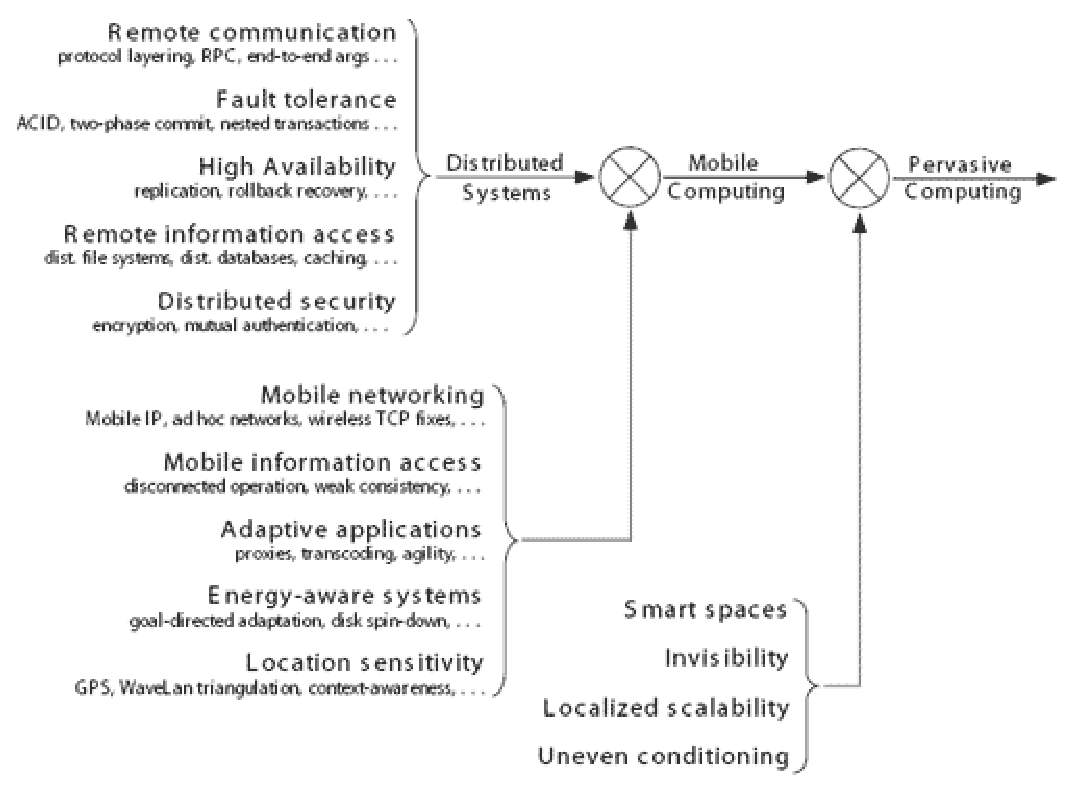
\includegraphics[width=0.8\textwidth]{images/pervasive_computing.eps}
  \caption[Caption for LOF]{Ο Διάχυτος Υπολογισμός ως συνδυασμός επιστημών\footnotemark}
  \label{fig:pervasive}
\end{figure}

Ένα από τα πιο σημαντικά, αν όχι το πιο σημαντικό, εργαλεία του Διάχυτου Υπολογισμού είναι τα Ασύρματα Δίκτυα Αισθητήρων(ΑΔΑ).
Τα ΑΔΑ αποτελούνται από έναν μεγάλο αριθμό κόμβων οι οποίοι καλύπτουν επαρκώς το περιβάλλον το οποίο είναι σε επιτήρηση.
Είναι το υποσύστημα το οποίο καταγράφει όλες τις πληροφορίες από το περιβάλλον αλλά και ταυτόχρονα είναι το ίδιο υποσύστημα που εκτελεί τις λειτουργίες που είναι
απαραίτητες κάθε στιγμή.
Ένα από τα κρισιμότερα συστατικά των ΑΔΑ είναι ο αισθητήρας: είναι το υποσύστημα του κόμβου το οποίο μετατρέπει μια φυσική ποσότητα όπως η υγρασία, η θερμοκρασία
κλπ σε ηλεκτρονικό δεδομένο.
Η επιστημονική κοινότητα από τις αρχές του 2000, αφού έχει μελετήσει σε βάθος τις προηγούμενες επιστήμες, σε σχέση με τα ΑΔΑ, όπως τα Δίκτυα, Ασύρματα Δίκτυα,
Κατανεμημένα Συστήματα κλπ έχει εστιάσει μεγάλο μέρος της προσοχή της στα Ασύρματα Δίκτυα Αισθητήρων αφού αποτελούν απαραίτητο εργαλείο για τον Διάχυτο Υπολογισμό.

\footnotetext{Η εικόνα παρουσιάζεται στην ιστοσελίδα του εργαστηρίου Διάχυτου Υπολογισμού του πανεπιστημίου Carnegie Mellon (CMU)}

Τα τελευταία αυτά 10 χρόνια, τα Ασύρματα Δίκτυα Αισθητήρων γνώρισαν τρομερή πρόοδο σε όλο το διάστημα. Εφευρέθηκαν μαθηματικά μοντέλα που προσομοιώνουν πλήρως τα
ΑΔΑ\cite{geometric_graphs}, αλγόριθμοι οι οποίοι εκμεταλλεύονται πλήρως τις ιδιότητές τους ώστε να έχουν καλύτερη απόδοση, άνω και κάτω φράγματα σε αποδόσεις
αλγορίθμων και πολλά άλλα.
Ο πιο σημαντικός περιορισμός τους, ο οποίος διαπιστώθηκε από την αρχή της έρευνας, είναι οι περιορισμένοι πόροι των κόμβων ειδικά σε θέματα ενέργειας.
Η περιορισμένη χωρητικότητα ενέργειας ενός κόμβου είναι το σημείο κλειδί το οποίο μάλιστα διαφοροποιεί τα ΑΔΑ από τα κλασσικά Ασύρματα Δίκτυα.
Επομένως η περισσότερη έρευνα πάνω στα ΑΔΑ, ακόμα και 10 χρονιά μετά, έχει σχέση με την ελαχιστοποίηση της κατανάλωσης της ενέργειας. Είναι πλέον αποδεκτό ότι με την
σημερινή τεχνολογία τα ΑΔΑ δεν γίνεται να λειτουργούν επ'άπειρον χωρίς την ανθρώπινη παρέμβαση κάτι που επηρεάζει σημαντικά το όραμα του Διάχυτου Υπολογισμού.
Διότι αν ο κάθε κόμβος σε ένα ΑΔΑ χρειάζεται ανθρώπινη παρέμβαση ανά τακτά χρονικά διαστήματα τότε το κόστος του συνολικού συστήματος αυξάνεται σημαντικά, ένας τομέας
που από την έναρξη μαζικής παραγωγής τέτοιων συστημάτων λαμβάνεται σοβαρά υπόψη και καθορίζει τελικά την επιτυχία τους. Όμως ακόμα και αν εξαιρέσουμε τον παράγοντα
του κόστους, ένα ΑΔΑ στο οποίο οι κόμβοι λόγω περιορισμένης ενέργειας διακόπτουν τη λειτουργία τους απρόσμενα μετά το ίδιο το δίκτυο γίνεται αναξιόπιστο
αποτυγχάνοντας τον αρχικό του στόχο: να βοηθά τον άνθρωπο.

Ωστόσο μια καινούργια τεχνολογία που εφευρέθηκε από τους επιστήμονες του MIT \cite{power_mit_1} έρχεται να αλλάξει άρδην τις προσδοκίες στο πεδίο των ΑΔΑ. Η
τεχνολογία
αυτή επιτρέπει την ασύρματη μετάδοση ενέργειας από μια Πηγή σε έναν δέκτη με πολύ μικρές απώλειες ενέργειας.






\section{Ασύρματα Δίκτυα Αισθητήρων(ΑΔΑ)}
Ένα Ασύρματο Δίκτυο Αισθητήρων(ΑΔΑ) αποτελείται από αυτόνομους κατανεμημένους κόμβους(ή αισθητήρες) όπου ο καθένας λαμβάνει μετρήσεις για το κοντινό του περιβάλλον,
όπως θερμοκρασία, υγρασία, επίπεδα θορύβου, σεισμικές δονήσεις, πίεση ακόμα και κίνηση με την προϋπόθεση πάντα ότι υπάρχει το απαραίτητο υλικό πάνω στον κόμβο ώστε
να μπορεί να λαμβάνει εκάστοτε μέτρηση.
Οι κόμβοι λαμβάνουν μετρήσεις περιοδικά με περίοδο που εξαρτάται από το είδος το δικτύου και ρυθμίζεται από τον αρχικό σχεδιαστή του δικτύου.
Για ένα δίκτυο οι κόμβοι μπορεί να λαμβάνουν μετρήσεις ανά μια ώρα ενώ σε κάποιο άλλο δίκτυο οι αισθητήρες μπορεί να λαμβάνουν μετρήσεις ανά ένα δευτερόλεπτο.
Σε ένα ΑΔΑ σχεδόν πάντα θεωρείται ότι υπάρχει ένα ακόμα πολύ σημαντικό στοιχείο: η Πηγή.
Ο κάθε κόμβος αφού λάβει και καταγράψει ένα μέγεθος μετρήσεων στέλνει τα δεδομένα αυτά, δομημένα σε πακέτα μέσα από ένα πρωτόκολλο δρομολόγησης, στην Πηγή
χρησιμοποιώντας ως διαμεσολαβητές άλλους κόμβους.
Θα πρέπει να αναφερθεί ότι ο κάθε κόμβος δεν γνωρίζει την συνολική διαδρομή που θα ακολουθήσουν τα πακέτα αλλά γνωρίζει μόνο τον πρώτο γείτονα στον οποίο στέλνει κάθε
φορά ένα πακέτο που έχει προορισμό την Πηγή. Ένα παράδειγμα ενός ασύρματου δικτύου αισθητήρων φαίνεται στην εικόνα \ref{fig:farm}.

\begin{figure}[h]
	\centering
	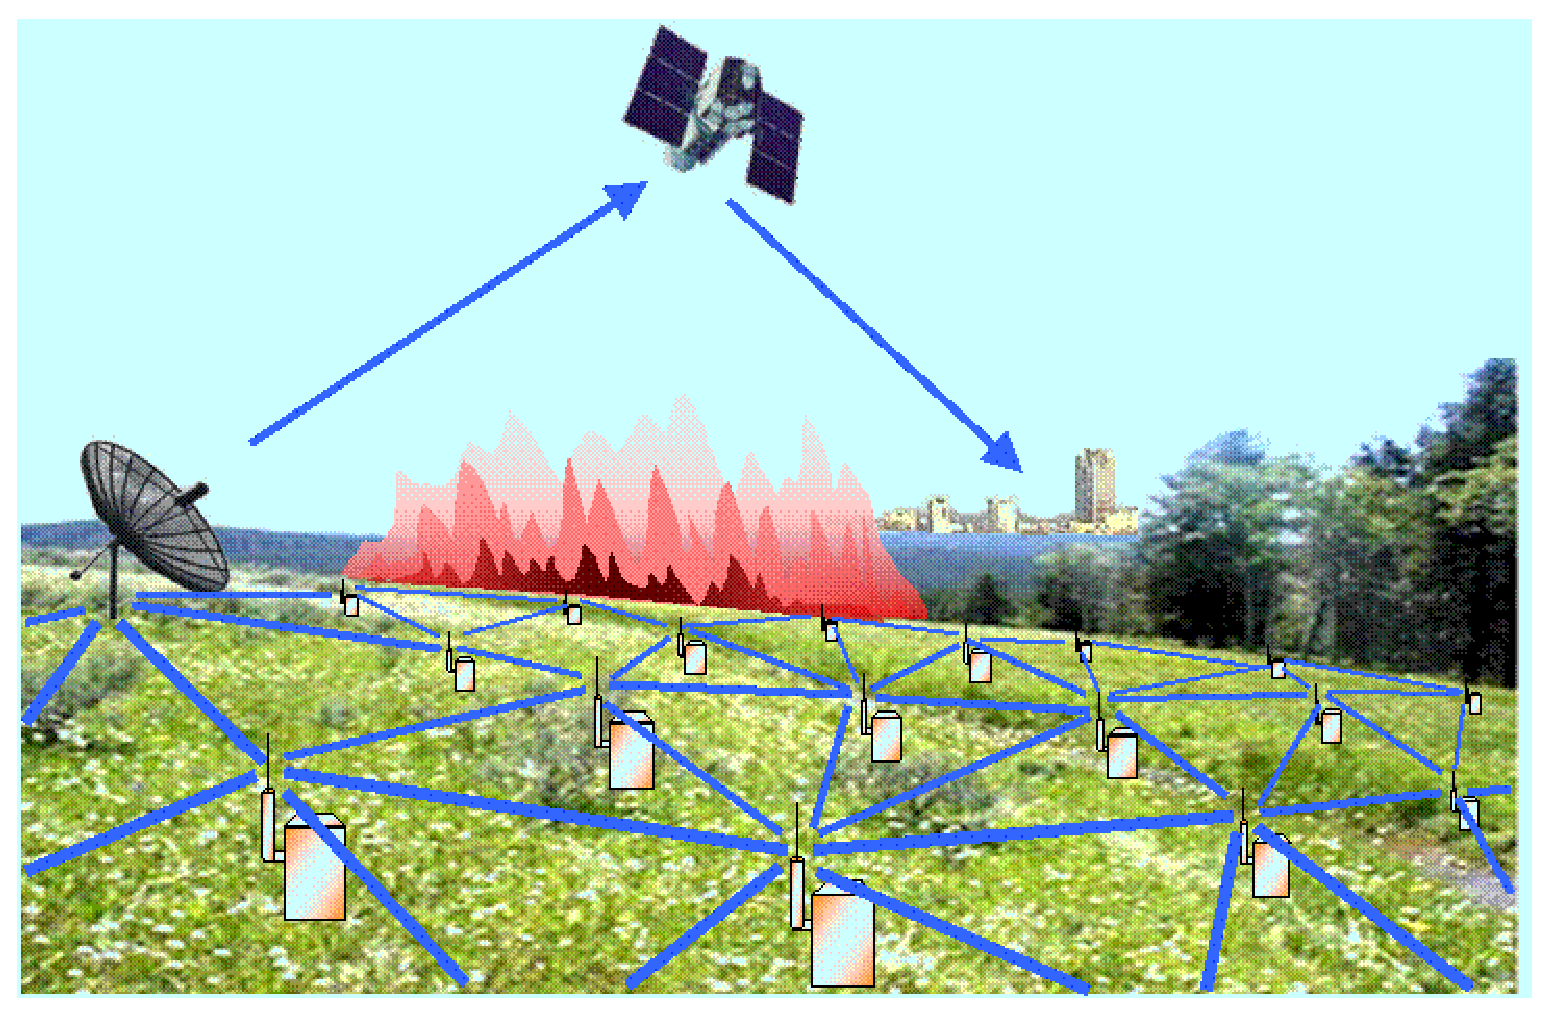
\includegraphics[width=0.9\textwidth]{images/sensor_network.eps}
	\caption{Ένα τυπικό σενάριο ενός ΑΔΑ}
	\label{fig:farm}
\end{figure}

Τα βασικά κριτήρια που χαρακτηρίζουν ένα δίκτυο ως ΑΔΑ είναι τα εξής:
\begin{itemize}
\item μεγάλοι περιορισμοί ως προς την κατανάλωση ενέργειας για τους κόμβους
\item ικανότητα του δικτύου να μπορεί να αντιμετωπίζει αποδοτικά δυσλειτουργίες και σφάλματα κόμβων
\item ικανότητα αντιμετώπισης αποτυχιών και προβλήματα επικοινωνίας μεταξύ κόμβων
\item ανομοιογένεια ως προς τους κόμβους
\item τοπικότητα στην πληροφορία
\item επεκτασιμότητα του δικτύου σε πολύ μεγάλα μεγέθη
\item εύκολη εγκατάσταση και χρήση του συνολικού δικτύου από έναν χειριστή
\end{itemize}
Ο αριθμός των κόμβων μπορεί να κυμαίνεται από μερικές εκατοντάδες μέχρι και αρκετές χιλιάδες.
Η κατανομή των κόμβων, δηλαδή ο τρόπος που τοποθετούνται, συνήθως είναι ομοιόμορφη αλλά αυτό δεν ισχύει πάντα. Για παράδειγμα έχει αποδεχτεί ότι μια διαφορετική
κατανομή όπως η Gaussian μπορεί να έχει καλύτερη απόδοση σε ένα ΑΔΑ, όσον αφορά κάποια συγκεκριμένα χαρακτηριστικά \cite{gaussian_sensors}.
Ο κάθε κόμβος αποτελείται συνήθως από κάποια τυπικά μέρη:
\begin{itemize}
\item πομπό/δέκτη που να χρησιμοποιεί χαμηλής ενέργειας ασύρματα πρωτόκολλα
\item μικροελεγκτή χαμηλής κατανάλωσης ενέργειας, από πολύ απλούς των 8bit μέχρι και σύγχρονους με μεγάλη υπολογιστική δύναμη. Το κύριο χαρακτηριστικό τους είναι η
μικρή κατανάλωση ενέργειας
\item μπαταρία και γενικά ένας πόρος ενέργειας
\item αισθητήρες όπως θερμόμετρο, βαρόμετρο, κάμερα κλπ
\end{itemize}
Αν και υπάρχει η τεχνολογία να φτιαχτεί το υλικό ενός κόμβου σε μέγεθος "ψείρας", οι μπαταρίες αυξάνουν δραματικά το μέγεθος ούτως ώστε ένας κόμβος να λειτουργεί
απροβλημάτιστα για πολύ καιρό.
Επίσης θα πρέπει να σημειωθεί ότι, αν και θεωρούμε ότι υπάρχουν κάποιοι περιορισμένοι πόροι όσον αφορά το υλικό όπως για παράδειγμα τις δυνατότητες
του μικροεπεξεργαστή και κατά συνέπεια του μικροελεγκτή που φέρει ένας κόμβος, στα ΑΔΑ δεν μελετώνται περιπτώσεις όπου οι κόμβοι δεν έχουν έλεγχο της κίνησής τους ή
δεν έχουν καθόλου μνήμη και ικανότητα εκτέλεσης βασικών πράξεων.
Τέτοιες περιπτώσεις υπάγονται σε άλλα μοντέλα όπως τα Πρωτόκολλα Πληθυσμών \cite{population_protocols}.

Η Πηγή είναι ένα ξεχωριστό στοιχείο του δικτύου, το οποίο έχει τεράστια υπολογιστική ικανότητα σε σχέση με τους κόμβους, δεν έχει κανέναν περιορισμό πόρων ενώ
ταυτόχρονα έχει εμβέλεια επικοινωνίας
πολύ μεγαλύτερη από τους κόμβους.
Σε μερικά δίκτυα η Πηγή συμμετέχει στο πρωτόκολλο δρομολόγησης ή βοηθάει μερικώς το συνολικό δίκτυο χρησιμοποιώντας τα ιδιαίτερα χαρακτηριστικά της.
Στην Πηγή φθάνουν τελικά όλες οι πληροφορίες και είναι υπεύθυνη για την διαχείριση αυτών των πληροφοριών όπως για παράδειγμα εκτέλεση ειδικών
επερωτημάτων (queries) επάνω στα δεδομένα για ασφαλή και γρήγορη εξαγωγή συμπερασμάτων για το δίκτυο.

Τα βασικά Ασύρματα Δίκτυα Αισθητήρων σταματάνε σε αυτό το σημείο.
Ο διαχειρισμός των δεδομένων καθώς και η εξαγωγή μετά-πληροφοριών από αυτά τα δεδομένα κλπ αποτελούν μέρη των διεπιστημονικών πεδίων του Διάχυτου Υπολογισμού και
Περιρρέουσας Νοημοσύνης.
Γίνεται επομένως σαφές λόγω του ότι τα ΑΔΑ αποτελούν το πιο κρίσιμο συστατικό για τις προαναφερθείσες επιστήμες.

Τέλος, να σημειωθεί ότι γενικώς στα ΑΔΑ θεωρείται ότι οι αισθητήρες έχουν συνεργατικές τάσεις, δηλαδή συνολικά το δίκτυο έχει κοινό στόχο.
Αντίθετα πολύ σπάνια μελετώνται περιπτώσεις όπου ο κάθε κόμβος κοιτάει μεμονωμένα και εγωιστικά το δικό του συμφέρον.
Η ανάλυση αυτών των περιπτώσεων χρησιμοποιεί συνήθως θεωρία παιγνίων \cite{game_theroy_sensor}, ενώ υποδεικνύει ένα πλήρως ανομοιογενές δίκτυο διαφορετικό από την
αρχική φιλοσοφία των ΑΔΑ.

\section{Το Κίνητρο και Σύντομη Ιστορία των ΑΔΑ} \label{sec:history}
Το βασικό κίνητρο των ΑΔΑ ήταν κατά κύριο λόγο οι στρατιωτικές εφαρμογές.
Επισκόπηση του πεδίου μάχης, αναγνώριση στόχων, παρακολούθηση και καταγραφή των στρατιωτικών δυνάμεων και των διαθέσιμων πυρομαχικών τους ήταν από τις πρώτες
εφαρμογές που είχαν πυροδοτήσει την απόσπαση κονδυλιών, από κυβερνήσεις ηγετικών κρατών, για την έρευνα τέτοιων μηχανισμών.
Συγκεκριμένα η πρώτη πραγματική έρευνα πάνω στα δίκτυα αισθητήρων ξεκίνησε μέσα στην δεκαετία του 1980 στην υπηρεσία του υπουργείου Αμύνης των Η.Π.Α, την DARPA
(Defense Advanced Research Projects Agency).
Η υπηρεσία αυτή ξεκίνησε ένα καινούργιο πρόγραμμα το οποίο λεγόταν Κατανεμημένα Δίκτυα Αισθητήρων (DSN, Distributed Sensor Networks).
Ταυτόχρονα το ARPANET (Advanced Research Projects Agency Network) δίκτυο ήταν πλήρως λειτουργικό με 200 πανεπιστήμια και ερευνητικά κέντρα συνδεδεμένα.
Η βασική ιδέα των DSN ήταν ένα δίκτυο πολλών κατανεμημένων συνδεδεμένων κόμβοι οι οποίοι συνεργάζονταν μεταξύ τους αλλά ο κάθε κόμβος λειτουργούσε ανεξάρτητος.
Το πρωτόκολλο δρομολόγησης που χρησιμοποιήθηκε βασιζόταν στην μέθοδο της πλημμύρας.

Αν συνυπολογισθεί ότι εκείνη την περίοδο δεν υπήρχαν προσωπικοί υπολογιστές, πόσο μάλλον φορητοί υπολογιστές, ενώ το Ethernet μόλις άρχιζε και αποκτούσε φήμη, το
πρόγραμμα DSN μάλλον ήταν πολύ φιλόδοξο.
Η τεχνολογία για την υλοποίηση αυτού του εγχειρήματος είχε βρεθεί σε ένα σχετικά πρόσφατο συνέδριο \cite{1978DSN}.
Ουσιαστικά περιελάμβανε έναν αισθητήρα ήχου, ικανότητα αποστολής και λήψης σημάτων χαμηλής ενέργειας και το απαραίτητο λογισμικού κατανεμημένου χαρακτήρα.
Επιστήμονες από το πανεπιστήμιο Carnegie Mellon (CMU), εστίασαν το ενδιαφέρον τους στη κατασκευή ενός λειτουργικού συστήματος το οποίο θα απευθυνόταν σε τέτοιες
συσκευές, δηλαδή συσκευές συνδεδεμένες σε ένα δίκτυο, στις οποίες υπάρχει εύκολη και ενιαία πρόσβαση στους κατανεμημένους πόρους ενός αξιόπιστου DSN συστήματος.
Το αποτέλεσμα αυτού του συστήματος ήταν να δημιουργηθεί το λειτουργικό σύστημα Mach το οποίο για την εποχή του είχε αρκετά πρωτοπόρα στοιχεία \cite{Mach} ενώ είχε
μάλιστα και κάποια περιορισμένη εμπορική επιτυχία.

Λίγο καιρό αργότερα, επιστήμονες στο πανεπιστήμιο MIT επικεντρώθηκαν στην αναγνώριση (εχθρικών) ελικοπτέρων μέσα από επεξεργασία ακουστικών σημάτων.
Το σύστημα που χρησιμοποιήσαν ήταν μικρόφωνα κατανεμημένα διάσπαρτα σε ένα χώρο τα οποία στέλναν τις πληροφορίες τους σε έναν κεντρικό υπολογιστή.
Χρησιμοποίησαν ευρετικούς αλγόριθμους και τεχνικές ταιριάσματος για να μπορέσουν να πετύχουν αποδεχτά αποτελέσματα στην αναγνώριση ελικοπτέρων.
Επιπλέον επέκτειναν το σύστημα DSN προσθέτοντας αλγόριθμους για επεξεργασία σημάτων και τεχνικών ταιριάσματος \cite{4789229}.
Για την επίδειξη του συστήματος το εργαστήριο Lincoln στο MIT κατασκεύασε ένα πραγματικό δοκιμαστικό σενάριο για την ακουστική αναγνώριση ελικοπτέρων χαμηλής πτήσης
και αεροπλάνων \cite{aircraft}.
Χρησιμοποιήθηκαν κόμβοι που στην πραγματικότητα ήταν μικρόφωνα τα οποία έστελναν με ασύρματη τεχνολογία τα σήματα ήχου σε 3 σταθερούς υπολογιστές(επεξεργαστής
MC68000, 256KB μνήμη και 512ΚΒ κοινή μνήμη).
Στην εικόνα \ref{fig:lincoln_lab} \cite{lincoln_report} φαίνεται το δοκιμαστικό σενάριο.
Τελικά το συνολικό σύστημα δούλεψε επιτυχώς και κατάφερε να εντοπίσει τα χαμηλής πτήσης ελικόπτερα και αεροσκάφη.
\begin{figure}[h]
	\centering
	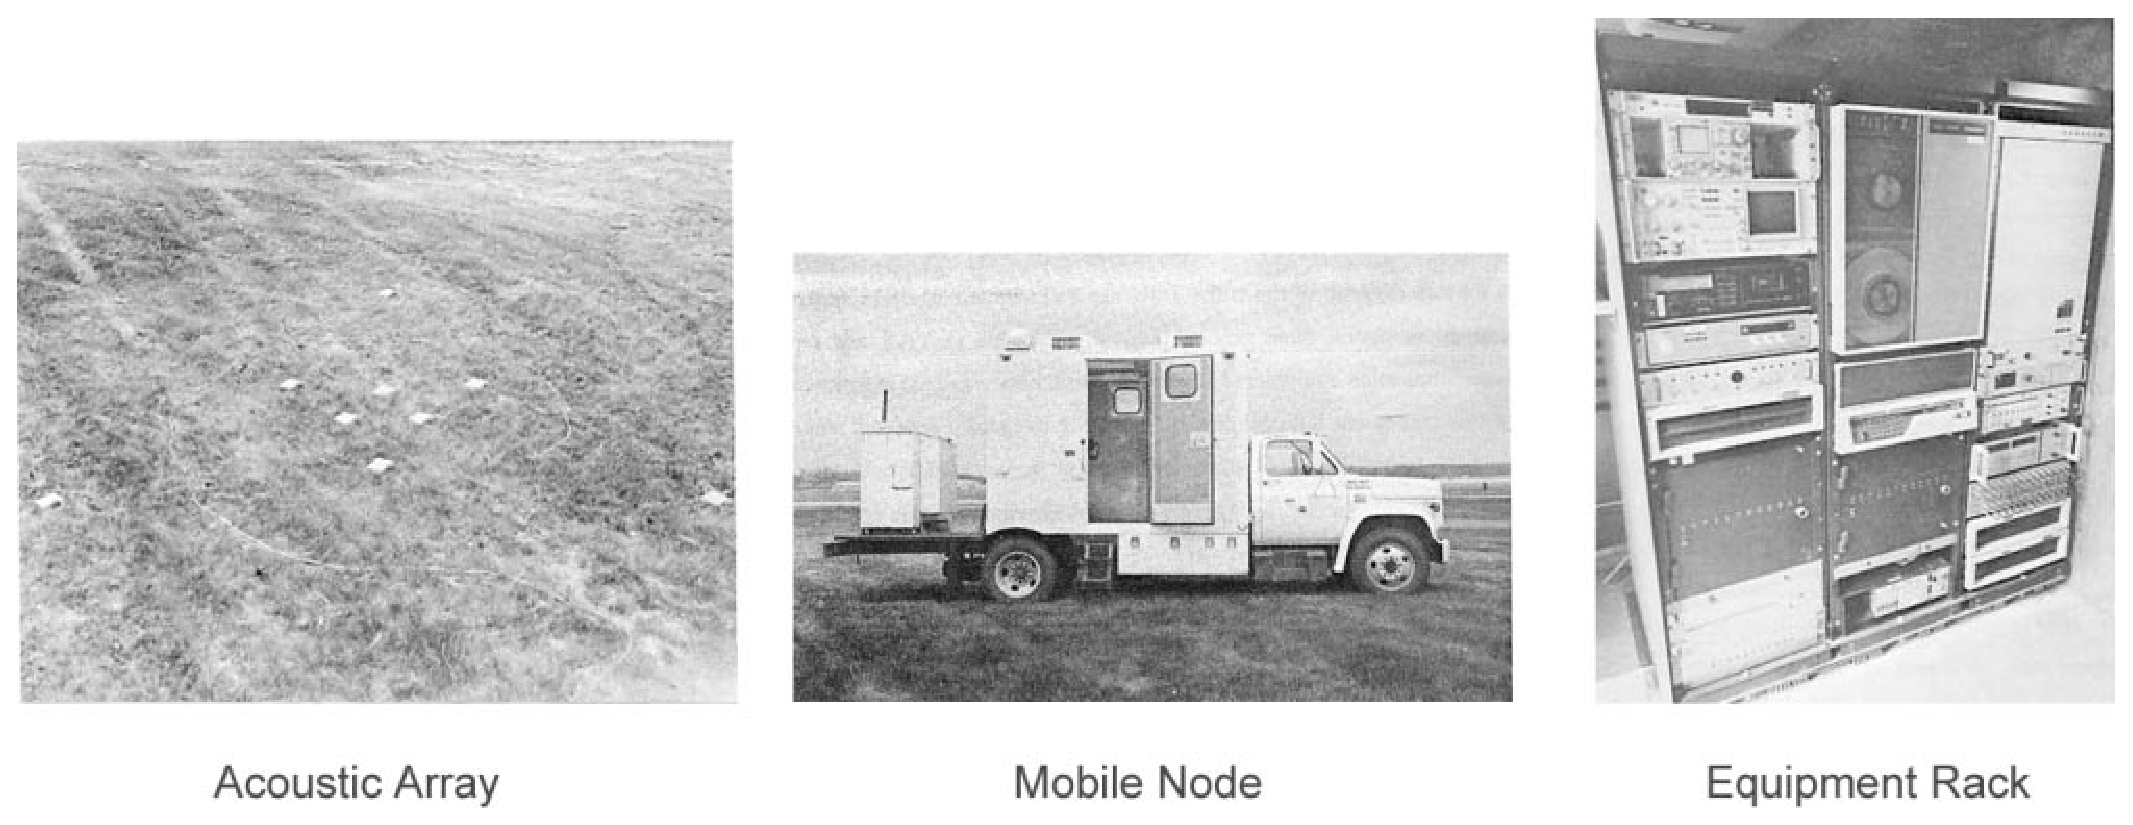
\includegraphics[width=0.8\textwidth]{images/lincoln_lab.eps}
	\caption{Tο δοκιμαστικό πείραμα του εργαστηρίου Lincoln του MIT}
	\label{fig:lincoln_lab}
\end{figure}

Ενώ οι ερευνητές είχαν κατανοήσει ότι τέτοια συστήματα θα έπρεπε να περιλαμβάνουν πολλά μικρά δίκτυα αισθητήρων τα οποία θα έχουν εκατοντάδες κόμβους, η τεχνολογία
για αυτά τα συστήματα δεν ήταν πλήρως έτοιμη.
Ωστόσο στρατιωτικοί παράγοντες είχαν αναγνωρίσει την τεράστια χρησιμότητα αυτών των συστημάτων καθώς και την υπερτερότητα των δικτυακών όπλων: χιλιάδες αισθητήρες που
συνεργάζονται και μαζεύουν πληροφορίες σε σχέση με τον εχθρό και τις αποστέλλουν στο κέντρο επιχειρήσεων, το οποίο μπορεί να είναι χιλιόμετρα μακριά από το πεδίο
μάχης.
Το προβάδισμα αυτό θα μπορούσε να λειτουργήσει μοιραία στην εξέλιξη μιας μάχης.

Το πρώτο πραγματικό σύστημα που υλοποιήθηκε με αυτόν τον σκοπό και έχει αρκετή σχέση με τα ΑΔΑ είναι το CEC (Cooperative Engagement Capability)\nocite{cec} το οποίο
κατασκευάστηκε από το ναυτικό των Η.Π.Α. στα μέσα της δεκαετίας του 1990.
Το σύστημα αποτελείται από πολλά ραντάρ τα οποία συλλέγουν πληροφορίες για στόχους αέρος όπως αεροσκάφη, ελικόπτερα πύραυλοι κλπ.
Οι μετρήσεις αυτές αποστέλνονται σε έναν κόμβο αρχηγό ( ουσιαστικά πρόκειται για μία Πηγή) ο οποίος επεξεργάζεται και φιλτράρει τις πληροφορίες.
Ο κόμβος αυτός είναι κοινός σε όλους τους άλλους κόμβους που μαζεύουν πληροφορίες.
Το σημαντικό στοιχείο του συστήματος είναι ότι όλοι οι κόμβοι έχουν πρόσβαση σε όλες τις πληροφορίες δημιουργώντας ένα πραγματικά κατανεμημένο σύστημα το οποίο δίνει
την ίδια εικόνα σε όλους τους στρατιωτικούς οι οποίοι βρίσκονται σε ένα κόμβο ο καθένας. Το σύστημα αυτό ακολούθησαν και άλλα στρατηγικά συστήματα με παρόμοιους
στόχους όπως το REΒMASS (Remote Battlefield Sensor System) και το TRSS (Tactical RemoteSensor System).


Ταυτόχρονα η τεχνολογία στους υπολογιστές εξελισσόταν ραγδαία.
Είχαν κατασκευαστεί ασύρματα δίκτυα, είχε δημιουργηθεί το Internet, οι μικροεπεξεργαστές είχαν πλέον αρκετή υπολογιστική ισχύ ενώ υπήρχε η δυνατότητα κατασκευής
μικρουπολογιστικών συστημάτων που είχαν μέγεθος όσο μια παλάμη.
Αυτές οι εξελίξεις σε συνδυασμό με τα οράματα της Περιρρέουσας Νοημοσύνης και του Διάχυτου Υπολογισμού έκαναν τους επιστήμονες να οραματιστούν μια διαφορετική πλευρά
τον δικτύων αισθητήρων: ασύρματα δίκτυα αισθητήρων τα οποία θα συλλέγαν πληροφορίες με στόχο να βοηθήσουν τον άνθρωπο.
Τα ΑΔΑ δηλαδή θα είχαν στόχο να κάνουν πιο εύκολη την ζωή του ανθρώπου από κάθε μεριά αναλαμβάνοντας αυτά κάποιες λειτουργίες σύμφωνα με τις πληροφορίες που έχουν
συλλέξει χωρίς όμως ο άνθρωπος να αλληλεπιδρά με το συνολικό σύστημα.
Έγινε όμως αμέσως αντιληπτό ότι τέτοια συστήματα θα ήταν άμεσα ευπαθή στην διαχείριση της ενέργειας.
Διότι ενώ όλες οι υπόλοιπες τεχνολογίες είχαν εξελιχθεί ραγδαία, η πρόοδος στις τεχνολογίες της μπαταρίας είχαν πολύ μικρότερη πρόοδο ενώ ταυτόχρονα τέτοια συστήματα
θα έπρεπε να λειτουργούν σχεδόν για πάντα χωρίς την αλληλεπίδραση του ανθρώπου.
Επίσης διαπιστώθηκε ότι αλγόριθμοι για τα κλασσικά ασύρματα δίκτυα (όπως ALOHA, slotted ALOHA κλπ) δεν θα μπορούσαν να χρησιμοποιηθούν καθώς τα ασύρματα δίκτυα έχουν
στόχο την μεγιστοποίηση της απόδοση ενώ τα ΑΔΑ έχουν στόχο την μεγιστοποίηση των χρονικών διαστημάτων που οι κόμβοι, με περιορισμένους πόρους ενέργειας, αποστέλλουν
πληροφορίες προς την Πηγή.

Από το 2000 και μετά η προσοχή της επιστημονικής κοινότητας επικεντρώθηκε κυρίως στην ελαχιστοποίηση της κατανάλωσης της ενέργειας στα ΑΔΑ είτε αυτό επιτυγχάνεται
μέσα από τα πρωτόκολλα δρομολόγησης είτε από τον τρόπο ανάπτυξης των αισθητήρων είτε με οποιαδήποτε άλλη τεχνική που θα μπορούσε να κάνει τα ΑΔΑ να αντισταθούν ακόμα
περισσότερο στο χρόνο.
Επίσης ξεκίνησαν να κατασκευάζονται μαζικά αισθητήρες οι οποίοι ήταν εμπορικά διαθέσιμη για πρακτικούς και ερευνητικούς σκοπός ενώ ταυτόχρονα δημιουργήθηκε το πρώτο
λειτουργικό σύστημα ειδικά για ΑΔΑ, το TinyOS.
Άμεσα οι  πρώτες πειραματικές εφαρμογές που δημιουργήθηκαν με τα ΑΔΑ οι οποίες αφορούσαν σχεδόν όλους τους τομείς της ανθρώπινης δραστηριότητας.

%\begin{comment}
\section{Ασύρματα Δίκτυα Αισθητήρων και οι Εφαρμογές τους}
Η τεχνολογία των Ασύρματων ∆ικτύων Αισθητήρων μπορεί να εφαρμοστεί σε πολλές εφαρμογές του πραγματικού κόσμου και να φέρει στην επιφάνεια κάποιες εντελώς καινούριες.
Ενα κρίσιμο και πρωτεύον συστατικό των κόμβων των ασύρματων δικτύων αισθητήρων είναι ο αισθητήρας.
Για πολλές παραμέτρους του φυσικού περιβάλλοντος υπάρχει η κατάλληλη τεχνολογία αισθητήρα που μπορεί να ενσωματωθεί σε ένα ΑΔΑ.
Οι πιο ευρέως χρησιμοποιούμενοι είναι οι αισθητήρες θερμοκρασίας, υγρασίας, ήχου, πίεσης και οι χημικοί αισθητήρες.
Μια σύντομη λίστα με τις πιο βασικές εφαρμογές παρουσιάζεται παρακάτω:
\begin{itemize}
\item \textbf{Πρόληψη Καταστροφών:} Μια από τις πιο συχνά αναφερόμενες εφαρμογές των ΑΔΑ είναι στην πρόληψη καταστροφών.
Ένα τυπικό σενάριο για εφαρμογές αυτής της κατηγορίας είναι η ανίχνευση πυρκαγιών.
Οι κόμβοι αισθητήρων είναι εξοπλισμένοι με θερμόμετρα και μπορούν να υπολογίσουν τη θέση τους τρέχοντας κάποιον αλγόριθμο εντοπισμού θέσης (localization).
Τους κόμβους αυτούς μπορούμε να τους απλώσουμε σε ένα δάσος, πετώντας τους από ένα αεροπλάνο. Έτσι σχηματίζεται ένας θερμοκρασιακός χάρτης της
περιοχής και σε περίπτωση υψηλών θερμοκρασιών και χαμηλής υγρασίας που υπονοούν πυρκαγιά ενημερώνουν τους πυροσβέστες.
\item \textbf{Έλεγχος του περιβάλλοντος και της βιοποικιλότητας:} Τα ΑΔΑ μπορούν να χρησιμοποιηθούν για να ελέγχουν το περιβάλλον ως προς τους χημικούς ρύπους
ή ακόμα και για το σχηματισμό μιας εικόνας ως προς τον αριθμό των διαφορετικών ειδών πανίδας και χλωρίδας μιας περιοχής.
\item \textbf{Ευφυή Κτίρια:} Τα μεγάλα κτίρια συχνά καταναλώνουν μεγάλα ποσά ενέργειας εξαιτίας λανθασμένης χρήσης των συσκευών Air Condtitioning (HVAC).
Μια αποδοτικότερη, πραγματικού-χρόνου και ακριβέστερη παρακολούθηση της θερμοκρασίας, της υγρασίας και άλλων παραμέτρων μπορεί να μειώσει την κατανάλωση ενέργειας.
Επίσης, μπορούν να χρησιμοποιηθούν για την παρακολούθηση των μηχανικών καταπονήσεων σε κτίρια ή γέφυρες που βρίσκονται σε σεισμικά ενεργές ζώνες, ενώ άλλου τύπου
αισθητήρες μπορούν χρησιμοποιηθούν για τον εντοπισμό εγκλωβισμένων ανθρώπων σε περιπτώσεις σεισμού.
Οι αισθητήρες μπορούν να τοποθετηθούν στα κτίρια τη στιγμή της κατασκευής τους ή αφού έχουν κατασκευαστεί.
Σε αυτές τις εφαρμογές η εξοικονόμηση ενέργειας για τους αισθητήρες είναι πολύ σημαντική απαίτηση.
\item \textbf{∆ιαχείριση Εγκαταστάσεων:} Τα ΑΔΑ μπορούν να χρησιμοποιηθούν για εφαρμογές διαχείρισης μεγάλων εγκαταστάσεων, όπως θέματα ασφαλείας.
Η είσοδος των ανθρώπων στις εγκαταστάσεις μπορεί να γίνεται χωρίς κλειδιά, αλλά με τη χρήση κάποιου πομπού, ενώ μπορούν να εντοπίζονται πιθανοί εισβολείς.
Επίσης σε χημικές εγκαταστάσεις τα ΑΔΑ θα μπορούσαν να χρησιμοποιηθούν για τον εντοπισμό διαρροών.
\item \textbf{Συντήρηση Μηχανών:} Αισθητήρες μπορούν να τοποθετηθούν σε δυσπρόσιτα σημεία μηχανών για να ελέγχουν τους κραδασμούς που υποδεικνύουν ανάγκη για
συντήρηση.
Παραδείγματα τέτοιων μηχανών είναι αυτόματες μηχανές ή οι άξονες των τροχών των τρένων.
\item \textbf{Εφαρμογές στη Γεωργία:} Η εφαρμογή ΑΔΑ σε καλλιεργήσιμες εκτάσεις με τοποθέτηση αισθητήρων μέτρησης υγρασίας και ανάλυσης της σύστασης του
εδάφους επιτρέπει την ακριβέστερη και αποδοτικότερη λίπανση και άρδευση των εκτάσεων.
Επίσης, η εκτροφή ζώων μπορεί να ωφεληθεί τοποθετώντας αισθητήρες στα ζώα που ελέγχουν την κατάσταση της υγείας τους.
\item \textbf{Εφαρμογές στον τομέα της υγείας:} Η χρήση ΑΔΑ στον τομέα της υγεία μπορεί να αποδειχτεί πολύ ωφέλιμη.
Όμως υπάρχουν αρκετά ηθικά διλήμματα πάνω στο θέμα αυτό.
Οι πιθανές εφαρμογές εκτείνονται από την άμεση τοποθέτηση αισθητήρων στον ίδιο τον ασθενή για την παρακολούθηση της υγείας του και ίσως αυτόματη χορήγηση φαρμάκων,
μέχρι την παρακολούθηση των ιατρών και των ασθενών στα νοσοκομεία.
\item \textbf{Ευφυή οδικά συστήματα:} Στα ευφυή οδικά συστήματα αισθητήρες τοποθετούνται στους δρόμους, ακόμα και στα κράσπεδα των δρόμων οι οποίοι
συλλέγουν πληροφορίες για την κίνηση και την κατάσταση του οδικού δικτύου γενικότερα και επικοινωνούν με τους οδηγούς δίνοντάς τους χρήσιμες πληροφορίες.
\item \textbf{Στρατιωτικές Εφαρμογές:} Τα ΑΔΑ μπορούν να είναι ενιαίο και αναπόσπαστο τμήμα των στρατιωτικών συστημάτων.
Τα χαρακτηριστικά των ΑΔΑ, όπως είναι η γρήγορη τοποθέτηση τους, η αυτό-οργάνωση και η ανοχή στα σφάλματα, τα μετατρέπουν σε μια πολλά υποσχόμενη τεχνολογία για τα
στρατιωτικά συστήματα.
Κάποιες από τις πιθανές στρατιωτικές εφαρμογές τους είναι η παρακολούθηση της κατάστασης των εξοπλισμών και των πολεμοφοδίων, η στενή παρακολούθηση του πεδίου της
μάχης, η αναγνώριση των εχθρικών δυνάμεων, η εκτίμηση των καταστροφών μετά από μάχη καθώς και ο εντοπισμός και η αναγνώριση χημικής, ατομικής ή βιολογικής επίθεσης.
\end{itemize}



\section{Περιβάλλοντα Ανάπτυξης Εφαρμογών}
Ένα δίκτυο αισθητήρων προκειμένου να είναι εύκολα προγραμματίσιμο και να δίνει πληθώρα επιλογών στον προγραμματιστή αλλά και στο χρήστη θα πρέπει να τρέχει ένα
λειτουργικό σύστημα (ΛΣ) το οποίο είναι φτιαγμένο ειδικά για συστήματα ΑΔΑ.
Να σημειωθεί ότι το λειτουργικό σύστημα θα πρέπει να καλύπτει τόσο τους χρήστες (οι οποίοι π.χ. θα θέλουν να τρέξουν ειδική εφαρμογή για την καλλιέργεια των φυτών
τους) αλλά και τους προγραμματιστές οι οποίοι θέλουν να φτιάξουν δυνατές και αξιόπιστες εφαρμογές εύκολα και σε σύντομο χρονικό διάστημα.
Γενικώς ένα λειτουργικό σύστημα προορισμένο για ασύρματα δίκτυα αισθητήρων θα πρέπει να έχει τα εξής χαρακτηριστικά:
\begin{itemize}
\item \textbf{Μικρή έκταση κώδικα:} Δεδομένης της περιορισμένης μνήμης ενός κόμβου, ο πυρήνας του λειτουργικού θα πρέπει να υλοποιηθεί με τον ελάχιστον δυνατό
κώδικα.
\item \textbf{Χαμηλή κατανάλωση ενέργειας:} Λόγω της φύσης και των περιορισμών των ΑΔΑ ένα ΛΣ προορισμένο για τα ΑΔΑ θα πρέπει να κάνει από μόνο του σωστή
διαχείριση των πόρων της ενέργειας.
\item \textbf{Αξιόπιστη αρχιτεκτονική:} Τα μονολιθικά ΛΣ πλέον θεωρούνται ξεπερασμένα λόγω της αρχιτεκτονικής τους. Τα σύγχρονα ΛΣ προκειμένου να προσφέρουν
αξιοπιστία θα πρέπει να έχουν αρχιτεκτονική μικροπυρήνα (micro-kernel).
Με αυτή την αρχιτεκτονική μόνο τα βασικά συστατικά του ΛΣ φορτώνονται στον πυρήνα ενώ όλα τα υπόλοιπα (σύστημα αρχείων, σύστημα επικοινωνίας κλπ) τρέχουν ως
διακομιστές (servers).
Επομένως αν κάποιο υποσύστημα πάθει βλάβη, όπως το σύστημα αρχείων, ενώ σε ένα μονολιθικό ΛΣ θα τίθονταν εκτός λειτουργίας όλος ο κόμβος, σε ένα ΛΣ αρχιτεκτονικής
μικροπυρήνα το σύστημα αρχείων θα έκανε μια επανεκκίνηση και ο κόμβος θα συνέχιζε την λειτουργία του.
\item \textbf{Εύκολο προγραμματιστικό μοντέλο:} Το προγραμματιστικό μοντέλο έχει σημαντική επιρροή στην δημιουργία εφαρμογών.
Tο πιο γνωστό προγραμματιστικό μοντέλο είναι το πολυνηματικό με χαμηλές απαιτήσεις σε πόρους \cite{os_sensors}.
\item \textbf{Αποδοτική χρονοδρομολόγηση:} Η χρονοδρομολόγηση ορίζει την διάταξη με την οποία εισέρχονται οι διαδικασίες στον πυρήνα του κεντρικού επεξεργαστή.
Επειδή όμως τα ΑΔΑ χρησιμοποιούνται σε πληθώρα εφαρμογών, υπάρχουν εφαρμογές που χρειάζονται ελαστική χρονοδρομολόγηση η οποία εξοικονομεί περισσότερη ενέργεια ενώ
άλλες χρειάζονται, λόγω της φύσης τους, χρονοδρομολόγηση πραγματικού χρόνου η οποία εξαντλεί την ενέργεια ενός κόμβου γρηγορότερα.
Το ΛΣ θα πρέπει να επιτρέπει στον προγραμματιστή τον τύπο της χρονοδρομολόγησης που θέλει να χρησιμοποιήσει.
\item \textbf{Αφηρημένη διεπαφή επικοινωνίας:} Η διεπαφή επικοινωνίας αναφέρεται τόσο στην επικοινωνία των διεργασιών μέσα σε έναν κόμβο όσο και στην επικοινωνία
μεταξύ των κόμβων.
Επειδή οι κόμβοι μπορεί να είναι τελείως ετερογενής μεταξύ τους, με άλλο υλικό και αρχιτεκτονική ο καθένας τους, το λειτουργικό σύστημα θα πρέπει να αφαιρέσει
τέτοιες λεπτομέρειες από την διεπαφή του προγραμματιστή.
\end{itemize}

Όπως φάνηκε και στο κεφάλαιο \ref{sec:history} από το ξεκίνημα των ΑΔΑ οι επιστήμονες προσπαθούσαν να δημιουργήσουν ένα λειτουργικό σύστημα το οποίο να έχει
χαρακτηριστικά παρόμοια με αυτά που αναφέρθηκαν.
Τα πρώτο λειτουργικό το οποίο χρησιμοποιήθηκε μαζικά ήταν το TinyOS το 2000.
Μετέπειτα δημιουργήθηκαν και άλλα ΛΣ για δίκτυα αισθητήρων καθένα με διαφορετικό κίνητρο και στόχο.
Συνοπτικά τα πιο γνωστά λειτουργικά συστήματα για δίκτυα αισθητήρων είναι τα εξής:

\begin{itemize}
\item \textbf{TinyOS:} Αναπτύχθηκε από το πανεπιστήμιο του Berkeley σε συνεργασία με την Intel και την Crossbow Technology.
Είναι ανοιχτού κώδικα και πρώτη έκδοσή του κυκλοφόρησε το 2000.
Υποστηρίζει έναν τεράστιο αριθμό από πλατφόρμες υλικού ενώ οι απαιτήσεις του σε μνήμη RAM είναι μόλις 2KB.
Η ανάπτυξη εφαρμογών TinyOS γίνεται στην γλώσσα nesC (Network Embedded Systems C) μία παραλλαγή της C αλλά με αντικειμενοστραφή χαρακτηριστικά και προορισμένη ειδικά
για ΑΔΑ \cite{tinyos}.
\item \textbf{Contiki:} Είναι ένα μικρό, ανοιχτού κώδικα, πολυνηματικό και πλήρως φορητό ΛΣ σχεδιασμένο ειδικά για συσκευές με περιορισμένους πόρους.
Μία τυπική εγκατάσταση χρειάζεται μόλις 2KB RAM και 40 KB ROM.
Είναι γραμμένο σε C, υποστηρίζει πλήρως το IPv6 ενώ μπορεί να εγκατασταθεί γραφικό περιβάλλον, περιηγητής, web server και πολλά ακόμα.
Η πρώτη έκδοση κυκλοφόρησε το 2005 ενώ έχει μεγάλη κοινότητα που ασχολείται με την περαιτέρω ανάπτυξή του \cite{contiki}.
\item \textbf{Mantis:} Πολυνηματικό λειτουργικό σύστημα ειδικά σχεδιασμένο για μικροελεγκτές με πολύ περιορισμένους πόρους.
Συγκεκριμένα μπορεί να τρέξει ακόμα και με 500Bytes RAM ενώ απαιτεί μόλις 14KB μνήμη ROM.
Ο δρομολογητής κάνει αποδοτική χρήση της διαθέσιμης ενέργειας θέτοντας σε λειτουργία ύπνου τον μικροελεγκτή όποτε χρειάζεται.
Είναι γραμμένο σε γλώσσα C \cite{mantis}.
\item \textbf{SOS:} Το λειτουργικό σύστημα αναπτύχθηκε στα πλαίσια ενός έργου του πανεπιστημίου UCLA σε συνεργασία με άλλα πανεπιστήμια.
Το κύριο κίνητρο για την ανάπτυξή του ήταν το γεγονός ότι μια εφαρμογή για ένα λειτουργικό σύστημα ΑΔΑ είχε άμεση σχέση με το ίδιο το ΛΣ.
Επομένως η μεταφορά του σε άλλο ΛΣ ήταν απαγορευτική.
Το ΛΣ SOS έχει δημιουργήσει διεπαφές οι οποίες συναντούνται στα σύγχρονα λειτουργικά συστήματα όπως run-time error checking, garbage collection κλπ.
Έχει μεταφερθεί σε μικροελεγκτές αλλά η ανάπτυξή του γίνεται με αργά βήματα κυρίως λόγω περιορισμένης χρήσης του \cite{sos_os}.
\item \textbf{Nano-RK:} Αναπτύχθηκε από το πανεπιστήμιο Carnegie Mellon με πλήρη υποστήριξη multi-hop δικτύου.
Υποστηρίζει τις πλατφόρμες FireFly και MicaZ.
Περιλαμβάνει πυρήνα πολύ μικρού μεγέθους αλλά με αρκετές δυνατότητες ενώ μπορεί να τρέξει σε συστήματα με 2KB RAM και 18KB ROM.
Υποστηρίζει σταθερής προτεραιότητας preemptive δρομολογητή διασφαλίζοντας έτσι ότι όλες οι προθεσμίες συναντώνται.
Το ΛΣ μπορεί να μειώσει την κατανάλωση ενέργειας μέσω της ιδιότητας που παρέχει οι εφαρμογές να μπορούν να ορίσουν τις απαιτήσεις τους σε πόρους που θα χρειαστούν
κατά την εκτέλεσή τους \cite{nano-rk}.
\item \textbf{Mat\'e:} Η βασική ιδέα αυτού του εγχειρήματος είναι να φτιαχτεί μια εικονική μηχανή(virtual machine) που να μπορεί να εγκατασταθεί επάνω από ΛΣ για
δίκτυα αισθητήρων.
Επομένως το Mat\'e θα λειτουργούσε όπως η Java λειτουργεί στα σύγχρονα λειτουργικά συστήματα.
Όμως ενώ η Java προσφέρει σωρεία από κλάσεις δημιουργεί ένα πολύ μεγάλο αρχείο bytecode απαγορευτικού μεγέθους για τους μικροελεγκτές που χρησιμοποιούνται στα ΑΔΑ.
Αντίθετα η ιδέα στο Mat\'e είναι ότι θα επιτρέπει στο χρήστη να επιλέξει σε ποια γλώσσα προγραμματισμού θα γράψει το
πρόγραμμά του, ποιες κλάσεις να συμπεριλάβει κλπ ώστε να μειωθεί το μέγεθος της εικονικής μηχανής και του τελικού αρχείου bytecode \cite{mate}.
\end{itemize}

Φυσικά υπάρχουν και άλλα εργαλεία για την γρήγορη ανάπτυξη εφαρμογών σε λειτουργικά συστήματα ΑΔΑ.
Για παράδειγμα έχουν αναπτυχθεί αναπτυχθεί εξομοιωτές διακριτού χρόνου όπως ο ns-2 \cite{ns-2} και ο νεότερος ns-3 \cite{ns-3}, ο OMNeT++ \cite{omnet}, o NetSim
\cite{netsim} και ο J-Sim \cite{j-sim}.
Παράλληλα έχουν αναπτυχθεί frameworks που περιέχουν έτοιμες υλοποιήσεις αλγορίθμων και μοντέλων για δίκτυα αισθητήρων και ασύρματα δίκτυα γενικότερα.
Ένα από τα πιο γνωστά είναι το wiselib \cite{wiselib}, μια βιβλιοθήκη η οποία περιέχει συναρτήσεις για αλγορίθμους δρομολόγησης, localization, κατανεμημένους
αλγόριθμους κλπ ενώ παρέχει πλήρη υποστήριξη για όλες σχεδόν τις πλατφόρμες δικτύων αισθητήρων.


\section{Σχεδιασμός Δικτύου, Προκλήσεις και το Μέλλον}\label{sc:wsn_design}
Κατά το σχεδιασμό ενός νέου δικτύου αισθητήρων ο σχεδιαστής έχει μια πληθώρα επιλογών να κάνει ώστε να πετύχει το βέλτιστο αποτέλεσμα σε σχέση με τις απαιτήσεις
του.
Στην βιβλιογραφία υπάρχουν άρθρα που μελετάνε κάθε πρόβλημα των ΑΔΑ ξεχωριστά αλλά κρατάνε όλους τις άλλες παραμέτρους σταθερές.
Επομένως όταν ο σχεδιαστής αναμίξει διάφορους αλγορίθμους και μοντέλα κατά την σχεδίαση (πχ έναν αλγόριθμο για την δρομολόγηση των πακέτων και ένα μοντέλο για την
τοπολογία του δικτύου) μπορεί να έχει χειρότερα αποτελέσματα από τα αναμενόμενα.
Οι πιο σημαντικές παράμετροι που ένας σχεδιαστής θα πρέπει να ρυθμίσει είναι οι εξής:
\begin{itemize}
\item \textbf{Ανάπτυξη των κόμβων:} Καθώς οι κόμβοι σε ένα ΑΔΑ γίνονται ολοένα και μικρότεροι, η ανάπτυξή τους μέσα σε έναν χώρο μπορεί να γίνει με πολλούς τρόπους.
Για παράδειγμα μπορούν να αναπτυχθούν ομοιόμορφα τυχαία (π.χ. να ριχθούν από ένα αεροπλάνο) ή να εγκατασταθούν σε συγκεκριμένα σημεία το οποίο είναι πιο
δύσκολο ειδικά αν ο αριθμός των κόμβων είναι μεγάλος.
Όμως η ανάπτυξη των κόμβων μπορεί να είναι συνεχόμενη.
Για παράδειγμα σε ένα ΑΔΑ μπορεί να διαπιστωθεί ότι μετά από κάποιο καιρό λειτουργίας ένα σημείο ίσως χρειάζεται περισσότερους κόμβους για να το επιβλέπουν.
Ο τρόπος που θα τοποθετηθούν τελικά οι κόμβοι (δηλαδή αν θα είναι ομοιόμορφοι ή ανομοιόμορφη η κατανομή τους) επηρεάζει σημαντικά την απόδοση του δικτύου.
\item \textbf{Κινητικότητα:} Η κινητικότητα μπορεί να είναι απρόσμενη (π.χ. μέσω του αέρα ή του νερού) ή να είναι προσχεδιασμένη για μερικούς κόμβους.
Η κίνηση μερικών κόμβων σε ένα δίκτυο μπορεί να βελτιώσει σημαντικά την απόδοση του δικτύου αφού μέσω της κίνησής τους μπορούν να ξεκουράζουν τους υπόλοιπους κόμβους
πηγαίνοντας πολύ κοντά σε αυτούς και παίρνοντας τα δεδομένα τους.
Όμως οι κόμβοι που κινούνται θα πρέπει να έχουν μεγάλους πόρους ενέργειας ή να μπορούν να επαναφορτίζονται με κάποιο τρόπο γιατί αλλιώς η ενέργειά τους θα τους
τελειώσει πολύ πιο γρήγορα από την ενέργεια των υπολοίπων κόμβων.
\item \textbf{Κόστος, Αριθμός κόμβων και Διαθέσιμοι πόροι:} Οι 3 έννοιες αυτές είναι αλληλένδετα συνδεδεμένες.
Μεγαλύτερο μέγεθος δικτύου, δηλαδή περισσότεροι κόμβοι, ή μεγαλύτερο μέγεθος διαθέσιμων πόρων συνεπάγεται άμεσα στην δραματική αύξηση του κόστους.
Κρατώντας το κόστος του δικτύου σταθερό ο σχεδιαστής θα πρέπει να επιλέξει μεταξύ μεγάλου αριθμού κόμβων και μεγάλων διαθέσιμων πόρων, κυρίως ενέργειας.
\item \textbf{Τύπος κόμβων} Ένα ακόμα στοιχείο το οποίο έχει άμεση σχέση με το κόστος του δικτύου αλλά ταυτόχρονα και με την λειτουργία και τον σκοπό του ΑΔΑ.
Χαρακτηριστικά των κόμβων περιλαμβάνουν την αρχιτεκτονική τους (π.χ. επεξεργαστής, μεγέθη RAM και ROM) αλλά και τις δυνατότητες επικοινωνίας τους όπως Wifi,
Zigbee, Laser, Bluetooth, IrDA κλπ.
\item \textbf{Ομοιογένεια κόμβων:} Αν και συνήθως τα ΑΔΑ κατασκευάζονται από ίδιο τύπο κόμβων αυτό δεν είναι ο κανόνας.
Ένας σχεδιαστής δικτύου μπορεί να προτιμήσει να εισάγει 80\% φθηνών κόμβων και 20\% ακριβότερων οι οποίοι όμως να έχουν ιδιαίτερα χαρακτηριστικά όπως κίνηση ή GPS που
τελικά το δίκτυο να έχει καλύτερη απόδοση.
\item \textbf{Κάλυψη του χώρου:} Ανάλογα με τον σκοπό ενός ΑΔΑ διαφορετικές πολιτικές κάλυψης είναι αναγκαίες.
Για παράδειγμα αν ένα ΑΔΑ πρέπει να εντοπίζει κινούμενες οντότητες μέσα στον χώρο του τότε θα πρέπει το κάθε σημείο να είναι τουλάχιστον 3-φορές καλυμμένο (δηλαδή
τουλάχιστον 3 κόμβοι να το αντιλαμβάνονται μέσω αισθητήρων) έτσι ώστε να μπορούν να δουλέψουν αλγόριθμοι localization και να μπορεί να βρεθεί η ακριβής θέση της
οντότητας.
Αντίθετα αν κάτι τέτοιο δεν είναι απαραίτητο τότε 1-φορά ή 2-φορές κάλυψη είναι αρκετή για τις ανάγκες του δικτύου.
\end{itemize}

Ο σχεδιασμός ενός ΑΔΑ έχει άμεση σχέση με την απόδοσή του. Ωστόσο η απόδοση έχει πολλές έννοιες ανάλογα με τον σκοπό του δικτύου. Οι βασικότερες μετρικές απόδοσης
είναι οι εξής:
\begin{itemize}
\item \textbf{Διάρκεια ζωής:} Ο πιο κρίσιμη αλλά ταυτόχρονα η πιο αμφιλεγόμενη μετρική απόδοσης. Αφηρημένα, η διάρκεια ζωής ενός ΑΔΑ ορίζεται το χρονικό διάστημα
μέχρι το δίκτυο να γίνει άχρηστο.
Στην βιβλιογραφία οι ορισμοί διαφέρουν σημαντικά.
Ορίζεται ως το χρονικό διάστημα μέχρι να πεθάνει ο πρώτος κόμβος του δικτύου ενώ υπάρχουν και ορισμοί που το ορίζουν ως το χρονικό διάστημα μέχρι να πεθάνει το 70\%
των κόμβων του δικτύου.
\item \textbf{Ομοιόμορφη κατανομή ενέργειας:} Μετρική που έχει άμεση σχέση με την διάρκεια ζωής ενός ΑΔΑ.
Μη ανομοιόμορφη κατανομή ενέργειας οδηγεί άμεσα κάποιους κόμβους να εξαντλήσουν την ενέργειά τους πολύ πιο γρήγορα από κάποιους άλλους.
Επομένως δημιουργούνται τρύπες (energy holes) στο δίκτυο οι οποίες μπορεί να σπάσουν το δίκτυο σε μικρότερες συνεκτικές συνιστώσες και ως αποτέλεσμα να χάνονται
πακέτα.
\item \textbf{Χρονοκαθυστέρηση (Latency):} Ορίζεται ο χρόνος που χρειάζεται από την στιγμή που δημιουργηθεί ένα γεγονός (event) στο δίκτυο μέχρι να το μάθει η Πηγή.
Εξαρτάται από τα hops του δικτύου αλλά γενικά είναι κλάσμα του δευτερολέπτου.
\item \textbf{Λόγος Επιτυχίας (Success rate):} Ορίζεται ως το ποσοστό των ληφθέντων γεγονότων στην Πηγή προς το ποσοστό των συνολικών γεγονότων που δημιουργήθηκαν στο
χώρο που καλύπτει
το ΑΔΑ.
Ή αλλιώς ο αριθμός των πακέτων που αποστάλθηκαν σωστά προς τον συνολικό αριθμό πακέτων που αποστάλθηκαν.
\item \textbf{Μέσος βαθμός των κόμβων (Node Degree):} Ορίζεται ως ο μέσος αριθμός των γειτόνων ενός κόμβου.
Έχει μεγάλη σημασία γιατί αν ο μέσος αριθμός γειτόνων είναι 1 με μικρή διασπορά τότε αν πεθάνει ένας κόμβος με μεγάλη πιθανότητα το δίκτυο θα σπάσει σε 2 μικρότερα
υποδίκτυα.
\end{itemize}
Φυσικά σε όλα αυτά θα πρέπει να συνυπολογίζεται κάθε φορά και η τυπική απόκλιση των εκάστοτε μετρικών.

Το όραμα που υπάρχει για τα ΑΔΑ για το μέλλον είναι ο κάθε άνθρωπος να μπορεί να αγοράσει και να εγκαταστήσει εκατοντάδες κόμβους εύκολα σε σημεία που χρειάζεται ο
ίδιος.
Οι κόμβοι αυτόματα θα ορίζουν αυτόματα πρωτόκολλα και τους αλγορίθμους που πρέπει να χρησιμοποιήσουν για την λειτουργία που έχουν επιλεχτεί.
Ο κάθε κόμβος θα πρέπει να είναι αθάνατος, δηλαδή να μην χρειάζεται ποτέ να αντικατασταθεί για πολύ μεγάλο χρονικό διάστημα.
Επίσης τα ΑΔΑ θα χρησιμοποιούνται πολύ στην παρακολούθηση πλανητών.
Εκεί ο κάθε κόμβος θα πρέπει να παραμένει ζωντανός για χρόνια ίσως και δεκαετίες.
Επομένως οι πλήρης εκμετάλλευση των μηχανισμών που βοηθούν τους κόμβους να κρατήσουν την ενέργειά τους για χρόνια είναι πάγια τοποθέτηση της επιστημονικής κοινότητας.
%this paragraph should end by showing the need for immortal WSNs !!
\section{Επισκόπηση της Διπλωματικής}
Στο κεφάλαιο \ref{ch:energy_reduction} παρουσιάζονται οι πιο γνωστές τεχνικές που χρησιμοποιούνται για την μείωση της κατανάλωσης της ενέργειας. Παρουσιάζονται
αποδοτικά πρωτόκολλα (αλγόριθμοι) δρομολόγησης καθώς και τα διάφορα είδη τους. Επίσης παρουσιάζονται πρωτόκολλα τα οποία κάνουν χρήση κινητών οντοτήτων, δηλαδή
συσκευές οι οποίες μπορούν να κινούνται στην περιοχή του δικτύου. Τέλος παρουσιάζονται εναλλακτικές τεχνικές όπως η εκμετάλλευση της ηλιακής ενέργειας και η μετέπειτα
αύξηση ή αύξηση των κόμβων του δικτύου ενώ γίνεται μία αναφορά στην ασύρματη μετάδοση ενέργειας.

Στο κεφάλαιο \ref{ch:wrsns} παρουσιάζεται πλήρως η τεχνολογία της ασύρματης μετάδοσης ενέργειας. Αρχικά γίνεται μια ιστορική αναδρομή γύρω από αυτήν την τεχνολογία (η
οποία έχει τις ρίζες της στον Νικόλα Τέσλα) και παρουσιάζεται η εξέλιξή της. Στην συνέχεια επεξηγείται πλήρως η λειτουργία της ασύρματης μετάδοσης ενέργειας καθώς και
οι ιδιότητές της.

Στο κεφάλαιο \ref{ch:strategies_solution} ορίζεται το πρόβλημα που πρέπει να λυθεί με την εμφάνιση της καινούργιας αυτής τεχνολογίας. Στην συνέχεια ορίζεται αυστηρά
το μοντέλο κάτω από το οποίο θα λυθεί το πρόβλημα και αποδεικνύεται ότι το πρόβλημα είναι υπολογιστικά δύσκολο, ότι δηλαδή ανήκει στην κλάση NP-πλήρης (NP-Complete)
των προβλημάτων. Τέλος παρουσιάζονται στρατηγικές επίλυσης, δηλαδή αποδοτικής διαχείρισης της συνολικής ενέργειας του δικτύου και ευρετικές τροχιές που θα μπορούσε να
ακολουθεί ο κινητός φορτιστής.

Στο κεφάλαιο \ref{ch:results} γίνεται η πειραματική αξιολόγηση των λύσεων που παρουσιάστηκαν στο κεφάλαιο 4. Αρχικά γίνεται σύγκριση ανάμεσα στο χρόνο ζωής ενός
ασύρματου δικτύου αισθητήρων χωρίς φόρτιση και ενός ΑΔΑ με φόρτιση. Στην συνέχεια γίνονται εκτεταμένα πειράματα ανάμεσα στις προτεινόμενες στρατηγικές και τις τροχιές
του κινητού φορτιστή.

Τέλος, στο κεφάλαιο \ref{ch:conclusion}, γίνεται μια επισκόπηση των αποτελεσμάτων που δίνονται και δίνονται προτάσεις για μελλοντικές εργασίες.


%\end{comment}
\label{ch:wsns}
%2nd chapter

\chapter{Τεχνικές Αύξησης της Διάρκειας Ζωής ενός ΑΔΑ}\label{ch:energy_reduction}


\section{Αποδοτικά Πρωτόκολλα Δρομολόγησης}
Η αποδοτική δρομολόγηση στα δικτυα αισθητήρων αποτελεί ένα από τα πιο προκλητικά προβλήματα λόγω των ιδιαίτερων χαρακτηριστικών που τα διαχωρίζουν από τα κλασσικά
δίκτυα και ασύρματα δίκτυα αισθητήρων.
Κατ'αρχήν πολλές φορές δεν είναι δυνατό να κτιστεί ένας καθολικός τρόπος διευθυνσιοδότησης λόγω του τεράστιου αριθμού των αισθητήρων.
Επομένως προτόκολλα τα οποία είναι βασισμένα στην διευθυνσιοδότηση IP δεν μπορούν να εφαρμοστούν στα δίκτυα αισθητήρων.
Δεύτερον, σε αντίθεση με τα κλασσικά δίκτυα δεδομένων, σχεδόν σε όλες τις εφαρμογές των ΑΔΑ απαιτούνται δεδομένα από πολλές διαφορετικές περιοχές ανίχνευσης τα
οποία προωθούνται σε μία συγκεκριμένη πηγή.
Επιπλέον, στα δεδομένα που αναπαράγονται μπορει να υπάρχει πλεονασμός πληροφοίας αφού πολλές μικρές περιοχές μπορεί να παράγουν τα ίδια δεδομένα.
Αυτός ο πλεονασμός πρέπει να εκμεταλευθεί από τα πρωτόκολλα δρομολόγησης αποδοτικά έτσι ώστε να επιτευχθεί μείωση της κατανάλωσης της ενέργειας και επέκταση του
χρόνου ζωής του δικτύου.
Στην συνέχεια θα περιγραφούν συνοπτικά τα πιο γνωστά προτόκολλα δρομολόγησης.


\subsection{Δεδομένο-κεντρικά πρωτόκολλα}
Όπως αναφέρθηκε σε ορισμένες εφαρμογές δεν είναι δυνατόν να ορίσουμε ξεχωριστά αναγνωριστικά (IDs) σε κάθε κόμβο ενός ΑΔΑ κυρίως λόγω του αριθμού των κόμβων.
Αυτή η αδυναμία σε συνδυασμό με την τυχαία ανάπτυξη των κόμβων καθιστούν αδύνατη την επιλογή ενός υποσυνόλου κόμβων για την απαίτηση
συγκεκριμένων πληροφοριών(queries).
Επομένως τα δεδομένα συνήθως μεταδίδονται από κάθε κόμβο και υπάρχει σημαντικός πλεονασμός πληροφορία.
Επειδή ο πλεονασμός καταναλώνει μεγαλύτερη ενέργεια σε ένα ΑΔΑ έχουν αναπτυχθεί δεδομένο-κεντρικά πρωτόκολλα δρομολόγησης τα οποία εκμεταλεύονται τον πλεονασμό
πληροφορίας για να επιλέξουν υποσύνολτα κόμβων. Τα πιο γνωστά δεδομενο-κεντρικά πρωτόκολλα δρομολόγησης είναι τα εξής:

\paragraph{Flooding και Gossiping:} Τα πρωτόκολλα πλημμύρας (flooding) και κουτσομπολιού (gossiping) \cite{gossiping} είναι δύο κλασσικοί μηχανισμοί για την μετάδοση
δεδομένων σε δίκτυα αισθητήρων χωρίς την χρήση κάποιου αλγορίθμου δρομολόγησης ή την συντήρηση κάποιας συγκεκριμένης τοπολογίας.
Στην μέθοδο πλημμύρας κάθε κόμβος μόλις λάβει ένα πακέτο δεδομένων το στέλνει σε όλους τους γείτονές του. Αυτή η διαδικασία συνεχίζεται μέχρι το πακέτο να φτάσει
στον προορισμό του ή όταν ο αριθμός των βημάτων (hops) που διήνυσε το πακέτο ξεπεράσει έναν συγκεκριμένο αριθμό (συνήθως την διάμετρο του δικτύου). Η μέθοδος του
κουτσοπολιού είναι μια λίγο πιο εξελιγμένη μορφή της μεθόδου πλημμύρας. Αντί ένας κόμβος, μόλις λάβει ένα καινούργιο πακέτο, να το στείλει σε όλους τους γείτονές του,
το στέλνει σε έναν γείτονα ο οποίος επιλέγεται τυχαία, ομοιόμορφα κατανεμημένα, από το σύνολο των γειτόνων του.

Παρόλο που τα δύο αυτά πρωτόκολλα μπορούν να υλοποιηθούν πάρα πολύ εύκολα, έχουν αρκετά μειονεκτήματα σχετικά με την απόδοσή τους. Συγκεκριμένα, η μέθοδος
πλημμύρας έχει πολύ μεγάλο πλεονασμό δεδομένων και επομένως σπαταλάει την ενέργεια του δικτύου. Αντίθετα, η μέθοδος κουτσομπολιού έχει πολύ μεγάλη καθυστέρηση αφού ο
τρόπος που επιλέγονται οι επόμενοι κόμβοι είναι τυχαίος.

\paragraph{SPIN:} Το πρωτόκολλο SPIN (Sensor Protocols for Information via Negotiation) \cite{spin_protocol} είναι από τις πρώτες εργασίες που έγιναν με στόχο να
χρησιμοποιηθεί ένας δεδομενο κεντρικός μηχανισμός για την δρομολόγηση στα δίκτυα αισθητήρων. Η ιδέα πίσω από το πρωτόκολλο SPIN είναι να ονομάζει τα δεδομένα,
χρησιμοποιώνας υψηλού επιπέδου περιγραφείς (descriptors) και μετα-δεδομένα (meta-data). Πριν την αποστολή κάποιου πακέτου δεδομένων, τα μετα-δεδομένα ανταλλάσονται
πρώτα ανάμεσα στους κόμβους μέσα από έναν μηχανισμό διαφήμησης. Κάθε κόμβος μολις λάβει ένα νέο πακέτο δεδομένων το διαφημίζει σε όλους τους γείτονές του. Οι γείτονες
που ενδιαφέρονται, ζητάνε τα δεδομένα να τους αποσταλούν.

Ένα από τα πλεονεκτήματα του πρωτοκόλου SPIN είναι οτι οι τοπολογικές αλλαγές είναι τοπικές αφού ο κάθε γείτονας χρειάζεται να ξέρει ουσιαστικά μόνο τους γείτονες
που είναι ένα hop μακριά. Επίσης η κατανάλωση ενέργειας μειώνεται κατα έναν παράγοντα 3.5 \cite{spin_protocol} σε σχέση με το πρωτόκολλο της πλημμύρας. Το μειονέκτημα
του πρωτοκόλλου είναι οτι ο μηχανισμός διαφήμησης που χρησιμοποιεί δεν επαρκεί για να υπάρχει κάποια εγγύηση στην παράδοση δεδομένων. Διότι αν ένας κόμβος
που ενδιαφέρεαι στα δεδομένα είναι πολύ μακρια απ τον κόμβο που τα παράγει τότε όλοι οι κόμβοι που βρίσκονται στο ενδιάμεσο δεν ενδιαφέρονται και επομένως τα δεδομένα
πολύ πιθανόν να μην παραδωθούν καθόλου στον προορισμό τους.

\paragraph{Directed Diffusion:}  Το πρωτόκολλο Directed Diffusion (DD) \cite{directed_diffusion} αποτελεί ένα σημαντικό ορόσημο στα δεδομενο-κεντρικά πρωτόκολλα και
στην έρευνα των δικτύων αισθητήρων. Η ιδέα στοχεύει στη διάχυση δεδομένων μέσα από τους κόμβους χρησιμοποιώντας ένα σχήμα ονομασίας για τα δεδομένα. Ο κύριος λόγος
για την χρησιμοποίηση ενός τέτοιου σχήματος είναι για να ξεφορτωθεί το πρωτόκολλο δρομολόγησης από άχρηστες εργασίες χαμηλότερων επιπέδων έτσι ώστε να εξοικονομηθεί
ενέργεια. Το πρωτόκολλο χρησιμοποιεί ζευγάρια ιδιότητας-τιμής σε αναθέσεις επερωτημάτων (queries). Προκειμένου να γίνει ένα επερώτημα, ένα "ενδιαφέρον" (interest)
ορίζεται χρησιμοποιώντας μια λίστα από τέτοια ζευγάρια όπως για παράδειγμα όνοματα αντικειμένων, διάστημα, διάρκεια, γεωγραφική περιοχή και άλλα. Το "ενδιαφέρον"
μεταδίδεται από την Πηγή προς όλες τις κατευθύνσεις (broadcast). Κάθε κόμβος αφού λάβει ένα "ενδιαφέρον" το αποθηκεύει στη μνήμη του για όσο καιρό είναι έγκυρο. Τα
"ενδιαφέροντα" στην μνήμη χρησιμοποιούνται για να συγκριθούν με τα ληφθέντα δεδομένα που έχουν τις συγκεκριμένες ιδιότητες και τιμές. Επίσης κάθε "ενδιαφέρον" έχει
κάποια επιπλέον πεδία που αφορούν τους συνδέσμους ανάμεσα σε έναν κόμβο και τους γείτονες που απάντησαν με δεδομένα σχετικά με το ενδιαφέρον. Tέτοια πεδία είναι η
ποιότητα του συνδέσμου, ο ρυθμός των εισερχόμενων δεδομένων η διάρκεια κ.α. Επομένως χρησιμοποιώντας αυτούς τους μηχανισμούς μπορούν να εγκατασταθούν πραγματικά
μονοπάτια μεταξύ των κόμβων που παράγουν δεδομένα και της Πηγής. Η Πηγή στο τέλος ξαναστέλνει το αυθεντικό πακέτο "ενδιαφέρον" χρησιμοποιώντας τα καινούργια
μονοπάτια. Με αυτόν τον τρόπο ουσιαστικά ενισχύει τα μονοπάτια αυτά τα οποία με μεγάλη πιθανότητα είναι και τα καλύτερα. Ένα παράδειγμα φαίνεται στην εικόνα
\ref{fig:dd_example}

\begin{figure}[h]
	\centering
	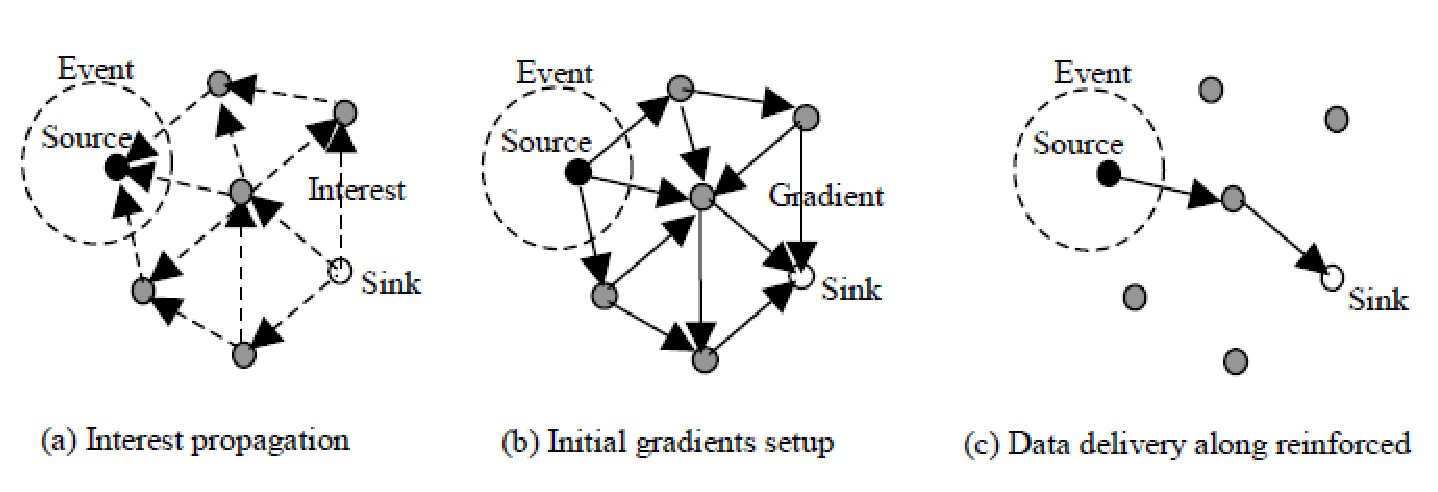
\includegraphics[width=\textwidth]{images/directed_diffusion.eps}
	\caption{Ένα σενάριο του πρωτοκόλλου Directed Diffusion.}
	\label{fig:dd_example}
\end{figure}

Το πρωτόκολλο Directed Diffusion διαφέρει από το SPIN ως προς το τρόπο που ζητάει τις πληροφορίες, δηλαδή τον τρόπο που θέτει τα επερωτήματα. Στο DD η πηγή θέτει
επερώτημα σε όλους τους αισθητήρες αν κάποια συγκεκριμένα δεδομένα είναι διαθέσιμα. Αν υπάρχουν τα δεδομένα ανάλογα με τα μονοπάτια που έχουν δημιουργηθεί, αυτά
ενισχύονται από την πηγή. Αντίθετα στο SPIN κάθε κόμβος διαφημίζει τα δεδομένα του στους υπόλοιπους κόμβους. Εαν κάποιος κόμβος ενδιαφέρεται τότε τα απαιτεί.Είναι
εμφανές οτι στο πρωτόκολλο DD υπάρχει υπεροχή όσον αφορά στην εξοικονόμηση ενέργειας ειδικά αν τα γεγονότα που εμφανίζονται στο δίκτυο έχουν μεγάλη διάρκεια. Όμως αν
τα γεγονότα έχουν πολύ μικρή διάρκεια τότε το DD έχει πολύ μικρή απόδοση αφού το \textbf{overhead} που θα υπάρχει μέχρι να στηθούν τα μονοπάτια θα είναι συγκρίσιμο με
την ενέργεια που σπαταλάται για να μεταφερθούν τα πραγματικά δεδομένα.

\paragraph{Rumor routing:} Η δρομολόγηση ανα φήμες (rumor routing) \cite{rumor_routing} είναι μια παραλλαγή του πρωτοκόλου Directed Diffusion και έχει κυρίως να κάνει
με ΑΔΑ στα οποία γεογραφικά κριτήρια δεν μπορούν να εφαρμοστούν. Γενικώς το DD πλημμυρίζει το δίκτυο με πακέτα προς όλους τους κόμβους μεχρι να φτιαχτούν τα
πραγματικά μονοπάτια τα οποία θα εμπεριέχουν ένα πολύ μικρό ποσοστό των συνολικών κόμβων του δικτύου. Αντίθετα στην δρομολόγηση ανα φήμες ο κάθε κόμβος προωθεί το
αναγνωριστικό πακέτο μόνο αν έχει "ακούσει" και ο ίδιος κάτι. Προσομοιώσεις έχουν δείξει οτι με αυτόν τον τρόπο εξοικονομείται περισσότερη ενέργεια στο δίκτυο
αισθητήρων μόνο όταν ο αριθμός των γεγονότων είναι σχετικά μικρός.

\paragraph{COUGAR:} Το αυτό δεδομενο-κεντρικό πρωτόκολλο είναι ριζοσπαστικό σε σχέση με τα υπόλοιπα καθώς βλέπει όλο το δίκτυο ως μια τεράστια, κατανεμημένα, βάση
δεδομένων \cite{cougar_protocol}. Η βασική ιδέα είναι να χρησιμοποιεί δηλωτικά ερωτήματα (declarative queries) με σκοπό να δημιουργήσει αφηρημένα επερωτήματα όπως η
επιλογή όλων των σχετικών κόμβων με μια πληροφορία κλπ. Αυτή η αφαίρεση γίνεται μέσα από ένα καινούργιο επίπεδο, αυτό των επερωτημάτων ανάμεσα στο επίπεδο δικτύου και
το επίπεδο των εφαρμογών. Όμως παρόλο που το επίπεδο αυτό είναι ανεξάρτητο του δικτύου έχει κάποια μειονεκτήματα. Κατ'αρχήν ένα επιπλέον επίπεδο στην στοίβα του
δικτύου θα καταναλώνει περισσότερη ενέργεια σε κάθε κόμβο. Επιπλέον, όπως και στις πραγματικές κατανεμημένες βάσεις δεδομένων, έτσι και εδώ θα πρέπει να λύνονται
αποδοτικά θέματα συγχρονισμού.

\subsection{Ιεραρχικά Πρωτόκολλα}
Όπως και στα κλασσικά δίκτυα ένα από τα πιο σημαντικά ζητήματα σχεδιασμού είναι αυτό της κλιμακωσιμότητας. Ένα "επίπεδο" δίκτυο μπορεί να προκαλέσει στην πύλη
δικτύου (gateway) υπερφόρτωση όταν το μέγεθος του δικτύου γίνει πολύ μεγάλο. Κατα συνέπεια η υπερφόρτωση μπορεί να προκαλέσει σοβαρή καθυστέρηση στις επικοινωνίες
και αντίστοιχα να χαθούν μερικά γεγονότα ή οι χρονικοί περιορισμοί που ορίζονται από αυτά. Ειδικά στην περίπτωση των ΑΔΑ όπου ο κάθε κόμβος έχει πολύ μικρή ακτίνα
εμβέλειας, η κλιμακωσιμότητα ενός "επίπεδου" πρωτοκόλλου δρομολόγησης είναι πολύ δύσκολη. Το πρόβλημα μπορεί να λυθεί εισάγοντας την έννοια της ιεραρχίας που πολλές
φορές γίνεται με μικρές συστάδες (clusters) σε όλη την περιοχή του δικτύου. Σε κάθε συστάδα συνήθως εκλέγεται ένας αρχηγός (cluster head) ο οποίος είναι υπεύθυνος για
την συστάδα του. Τα μέλη της συστάδας, κόμβοι του ΑΔΑ, ορίζονται από την ακτίνα εμβέλειας του αρχηγού όταν αυτός εκπέμψει ένα αναγνωριστικό μήνυμα. Αν σε έναν κόμβο
έρθει παραπάνω από ένα αναγνωριστικά μηνύματα τότε ο κόμβος θα γίνει μέλος της συστάδας της οποία το αναγνωριστικό σήμα είχε το καλύτερο (δυνατότερο) σήμα. Στην
συνέχεια παρουσιάζονται τα πιο γνωστά ιεραρχικά πρωτόκολλα δρομολόγησης.

\paragraph{LEACH:} Το πρωτόκολλο LEACH (Low-Energy Adaptive Clustering Hierarchy) \cite{leach_protocol} είναι ένα από τα πιο γνωστά ιεραρχικά πρωτόκολλα δρομολόγησης
για δίκτυα αισθητήρων. Η βασική ιδέα είναι να δημιουργηθούν συστάδες (clusters) βάση την ισχύ του ληφθέντος σήματος από τον αρχηγό. Οι κόμβοι της κάθε συστάδας,
χρησιμοποιώντας πολυ-βηματικές (multi-hop) μεταδόσεις, στέλνουν τα δεδομένα τους στον αρχηγό ο οποίος τα μαζεύει και τα στέλνει απευθείας στην πηγή. Με αυτόν τον
τρόπο μειώνεται η κατανάλωση της ενέργειας αφού μόνο οι αρχηγοί κάνουν μακρινές μεταδόσεις δεδομένων. Έχει υπολογιστεί οτι ο βέλτιστος αριθμός αρχηγών σε ένα δίκτυο
είναι περίπου το 5\% όλων των κόμβων του δικτύου. Προκειμένου να υπάρχει ακόμη μεγαλύτερη ισορροπία στην ενέργεια, οι αρχηγοί και κατα συνέπεια και οι συστάδες,
αλλάζουν ανα τακτά χρονικά διαστήματα. Συγκεκριμένα ένας κόμβος γίνεται αρχηγός με την παρακάτω πιθανότητα:

\begin{align*}
T(n) = \left\{
\begin{array}{cc}
 \frac{p}{1-p\cdot(r \text{mod}\frac{1}{p})} & \text{if } x<0 \\
  0 & \text{αλλιώς}
\end{array} \right.
\end{align*}
όπου $p$ είναι το επιθυμητό ποοστό των αρχηγών, $r$ είναι ο τρέχον γύρος και G είναι το σύνολο των κόμβων που δεν έχουν γίνει αρχηγοί τους προηγούμενους $\frac{1}{p}$
γύρους.

Το πρωτόκολλο LEACH μπορεί να πετύχει μέχρι και 7 φορές λιγότερη κατανάλωση ενέργειας σε σχέση με τα κλασσικά πρωτόκολλα ασύρματων δικτύων \cite{leach_protocol} ενώ
ακόμα και 12 χρόνια μετά την δημοσίευσή του παραμένει ένα από τα πιο κλασσικά πρωτόκολλα ΑΔΑ. Τα μόνα μειονεκτήματά του (τα οποία βελτιώθηκαν από επόμενες
δημοσιεύσεις) είναι οτι το μοντέλο που υποθέτει για την ακτίνα εμβέλειας των κόμβων, για πολύ μεγάλα δίκτυα, είναι μη ρεαλιστικό. Επίσης, για πολύ μεγάλα δίκτυα οι
αρχηγοί των συστάδων που βρίσκονται πολύ μακριά από την Πηγή εξαντλούν πολύ πιο γρήγορα την ενέργειά τους απ'ότι οι αρχηγοί των συστάδων που βρίσκονται κοντά στην
πηγή.

\paragraph{PEGASIS \& Hierarchical-PEGASIS:} Το πρωτόκολλο PEGASIS (Power-Efficient Gathering in Sensor Information Systems) \cite{pegasis_protocol} αποτελεί μια
βελτίωση του πρωτοκόλλου δρομολόγησης LEACH. Αντί να δημιουργούνται συστάδες, το PEGASIS σχηματίζει αλυσίδες με όλους τους κόμβους έτσι ώστε κάθε κόμβος λαμβάνει μόνο
από έναν κόμβο και αφού ενσωματώσει και τα δικά του δεδομένα τα αποστέλει σε μόνον έναν γείτονα. Ταυτόχρονα μόνο ένας κόμβος στην αλυσίδα έχει επιλεχτεί τυχαία ως
αρχηγός ο οποίος αναλαμβάνει να μαζέψει όλα τα δεδομένα και τα αποστέλει στην Πηγή. Η διαφορά από το LEACH είναι οτι χρησιμοποιεί πολυ-βηματικες (multi-hop)
μεταδόσεις μεταξύ των κόμβων και οτι μόνο ένας κόμβος σε κάθε γύρο είναι ο αρχηγός που αποστέλει τα δεδομένα στην Πηγή. Προσομοιώσεις δείξαν οτι μπορεί να βελτιώσει
ακόμα και 100\% την εξοικονόμηση ενέργειας σε σχέση με το LEACH. Το αρνητικό του όμως είναι οτι μπορεί τα πακέτα να έχουν μεγάλη καθυστέρηση μέχρι να φτάσουν στην
Πηγή. Το πρωτόκολλο Hierarchical-PEGASIS \cite{hierarchical_pegasis} αποτελεί μια προέκταση του PEGASIS το οποίο σκοπεύει στην μείωση της καθυστέρησης που
παρουσιάζεται στο PEGASIS. Ουσιαστικά δημιουργούνται περισσότερες από μια αλυσίδες με τον ίδιο προορισμό. Επίσης για την δημιουργία της αλυσίδας εφαρμοζει την μετρική
$energy\times delay$.

\paragraph{TEEN \& APTEEN:} Το πρωτόκολλο TEEN (The Energy Efficient sensor Network protocol) \cite{teen_protocol} είναι ένα
ιεραρχικό πρωτόκολο σχεδιασμένο να μπορεί να ανταποκρίνεται γρήγορα στις γρήγορες αλλαγές όπως είναι η θερμοκρασία με μεγάλη λεπτομέρεια. Η γρήγορη ανταπόκριση είναι
σημαντικό στοιχείο σε δίκτυα πραγματικού χρόνου. Οι συστάδες (clusters) σχηματίζονται παρόμοια με το LEACH πρωτόκολλο αλλά για για να πετύχει την γρήγορη ανταπόκριη,
το πρωτόκολλο ορίζει δύο κατώφλια που έχουν σχέση με τον τρόπο ανίχνευσης των γεγονότων από τους κόμβους. Το πρώτο ονομάζεται το σκληρό κατώφλι (hard threshold) και
ορίζει τις μικρότερες δυνατές τιμές μιας ιδιότητας που θα κάνουν τον κόμβο να "ξυπνήσει", δηλαδή να επανέλθει σε κανονική λειτουργία και να ενεργοποιήσει τον μεταδότη
του. Επομένως το σκληρό κατώφλι επιτρέπει τον κάθε κόμβο να αναφέρει δεδομένα μόνο όταν οι ιδιότητες αυτών ξεπεράσουν μια συγκεκριμένη τιμή που έχει να κάνει με το
πόσο ενδιαφέρον έχουν τα δεδομένα. Αντίθετα το μαλακό κατώφλι (soft threshold) επιτρέπει την μετάδοση δεδομένων μόνο όταν το ποσοστό των αλλαγών ξεπεράσουν την τιμή
του μαλακού κατωφλίου. Έτσι μειώνονται ακόμα περισσότερο οι μεταδόσεις πακέτων οι οποίες αφορούν πολύ μικρές αλλαγές στην περιοχή αίσθησης του κόμβου. Το μόνο
πρόβλημα που αντιμετωπίζει το πρωτόκολλο TEEN είναι όταν ο διαχειριστής του δικτύου επιθυμεί ο κάθε κόμβος να επιστρέφει πληροφορίες σε περιοδικό χρόνο. Το πρόβλημα
αυτό λύθηκε από μια προέκταση του TEEN, το ATEEN (Adaptive TEEN) \cite{apteen_protocol} στο οποίο μπορεί να ορίσει η πηγή με ποιον τρόπο θα γίνονται οι αναφορές από
κάθε κόμβο.


\subsection{Πρωτόκολλα Βασισμένα στην Τοποθεσία}
Πολλές φορές πρωτόκολλα για τα ΑΔΑ απαιτούν πληροφορίες για την τοποθεσία για τους κόμβους.
Στις περισσότερες περιπτώσεις οι πληροφορίες αυτές χρειάζονται για να υπολογιστούν οι αποστάσεις μεταξυ κόμβων και να εκτιμηθεί η ενέργεια που χρειάζεται για να
αποσταλή ένα πακέτο.
Επιπλέον, εφόσον δεν εφαρμόζονται πρωτόκολλα βασισμένα στην διευθυνσιοδότηση IP για τα δίκτυα αισθητήρων όπως συμβαίνει στα κλασσικά δίκτυα δεδομένων, ενώ ταυτόχρονα
οι κόμβοι είναι όλοι τοποθετημένοι σε μια συγκεκριμένη γεωγραφική περιοχή, πληροφορίες για την συγκεκριμένη τοποθεσία τους μέσα στην γεωγραφική περιοχή μπορούν
να χρησιμοποιηθούν για την δρομολόγηση δεδομένων και την μείωση της κατανάλωσης της ενέργειας.
Για παράδειγμα, αν η περιοχή που πρέπει να επιβλεφθεί για συγκεκριμένο σκοπό είναι γνωστή, χρησιμοποιώντας τις πληροφορίες τοποθεσίας των κόμβων, το επερώτημα (query)
προς το δίκτυο μπορεί να διοχετευθεί σε συγκεκριμένους κόμβους μόνο.
Αν και έχουν αναπτυχθεί αρκετά πρωτόκολλα τοπολογικής δρομολόγησης για τα κλασσικά ασύρματα δίκτυα αισθητήρων, αυτά δεν είναι εφαρμοσιμα στα ΑΔΑ καθώς η μετρική
απόδοσης που έχουν δεν περιλαμβάνει την μείωση της καταναλισκόμενης ενέργειας. Παρακάτω παρουσιάζονται τα πιο γνωστά πρωτόκολλα δρομολόγησης που βασίζονται στην
τοπολογία.


\paragraph{GAF:} Το πρωτόκολλο GAF (Geographic Adaptive Fidelity) \cite{gaf_protocol} είναι ένας ενεργειακός και βασισμένος στην τοπολογία αλγόριθμος δρομολόγησης
σχεδιασμένος αρχικά για ασύρματα δίκτυα αλλά πλέον εφαρμόζεται και σε ασύρματα δίκτυα αισθητήρων. Ο αλγόριθμος αυτός, εξοικονομεί ενέργεια απενεργοποιώντας περιττούς
κόμβους χωρίς να επηρεάζει την ποιότητα δρομολόγησης του δικτύου. Ο αλγόριθμος δημιουργεί ένα εικονικό πλέγμα (grid) για την περιοχή που καλύπτεται. Κάθε κόμβος
χρησιμοποιεί την τοποθεσία του για να συσχετίσει τον εαυτό του με κάποιο σημείο (τετράγωνο) του πλέγματος. Οι κόμβοι που είναι συσχετισμένοι με το ίδιο σημείο στο
πλέγμα θεωρούνται οτι είναι ισοδύναμοι όσον αφορά το κόστος της δρομολόγησης. Αυτή η ισοδυναμία εκμεταλεύεται απενεργοποιώντας μερικούς κόμβους και αφήνοντας μόνο
έναν ενεργοποιημένο σε κάθε σημείο (τετραγωνάκι) του πλέγματος. Ένα παράδειγμα φαίνεται στην εικόνα \ref{fig:gaf_example}. Συγκεκριμένα ο κόμβος 1 μπορεί να
επικοινωνήσει τους 2,3 και 4 και οι κόμβοι 2,3 και 4 μπορούν να επικοινωνήσουν με τον κόμβο 5. Επομένως οι κόμβοι 2,3 και 4 είναι ισοδύναμοι και οι δύο από αυτούς
μπορούν να απενεργοποιηθούν εξοικονομώντας ενέργεια.

\begin{figure}[h]
	\centering
	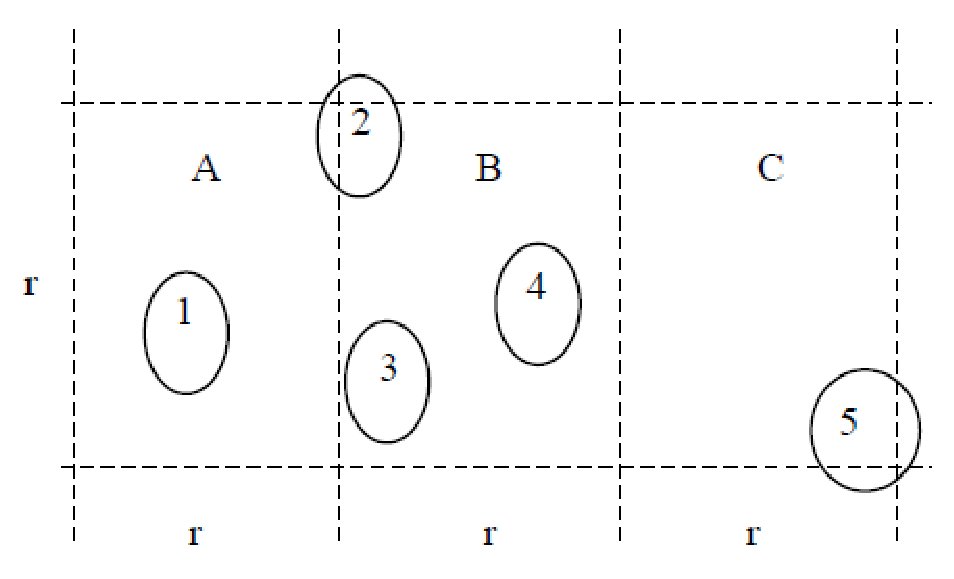
\includegraphics[width=0.6\textwidth]{images/gaf_example.eps}
	\caption{Ένα σενάριο του πρωτοκόλλου GAF.}
	\label{fig:gaf_example}
\end{figure}

Οι εξομοιώσεις έχουν δείξει οτι το πρωτόκολλο GAF μπορεί να έχει την ίδια απόδοση όσον αφορά την χρονοκαθυστέρηση (latency) και την απώλεια πακέτων σε σχέση με τα
κλασσικά πρωτόκολλα ασύρματων δικτύων, ενώ ταυτόχρονα αυξάνει την διάρκεια ζωής του δικτύου σε σημαντικό βαθμό.

\paragraph{GEAR: } Το πρωτόκολλο GEAR (Geographical and Energy Aware Routing) \cite{gear_protocol} προτείνει την χρησιμοποίηση γεγραφικών δεδομένων για την διάδοση
επερωτημάτων για συγκεκριμένες περιοχές αφού στις επερωτήσεις πολύ συχνά ενσωματώνονται γεωγραφικές ιδιότητηες. Το πρωτόκολλο χρησιμοποιεί ενεργιακές και γεωγραφικές
ευρετικές μεθόδους προκειμένου να δρομολογήσει κάποιο πακέτο. Η ιδέα είναι να περιορίσει τον αριθμό των πακέτων "ενδιαφέροντος" που χρησιμοποιεί το πρωτόκολλο
Directed Diffusion \cite{directed_diffusion} θεωρώντας μονο μια συγκεκριμένη περιοχή και όχι όλη την περιοχή του δικτύου. Στο πρωτόκολλο GEAR, κάθε κόμβος κρατάει
ένα κόστος εκτίμησης και ένα κόστος μάθησης της διαδρομής του πακέτου μέχρι τον προορισμό. Το κόστος εκτίμησης είναι ένας συνδυασμός την υπολοιπόμενης ενέργειας και
της απόστασης μέχρι τον προορισμό. Το κόστος μάθησης είναι ουσιαστικά το κόστος μάθησης αλλά λαμβάνει υπόψην και της ενεργειακές τρύπες του δικτύου που συμβαίνουν
όταν ένας κόμβος δεν έχει κανένα κοντινότερο γείτονα προς τον προορισμό εκτός από τον εαυτό του. Το κόστος μάθησης διαδίδεται ένα βήμα (hop) μακριά κάθε φορά που ένα
πακέτο φτάνει στον προορισμό του έτσι ώστε να χρησιμοποιηθεί στην επόμενη δρομολόγηση.


% \paragraph{GPSR:} Το πρωτόκολλο GPSR (Greedy Perimeter Stateless Routing for Wireless Networks)


\subsection{Πρωτόκολλα Εξισορόπισης Ενέργειας}
Όλα τα προηγούμενα πρωτόκολλα είχαν στόχο την μείωση της κατανάλωσης του δικτύου αισθητήρων και ως απώτερο σκοπό την επέκταση της διάρκειας ζωής του δικτύου.
Όμως πολλά από αυτά τα πρωτόκολλα δημιουργούν "παρενέργειες" σε ένα ΑΔΑ.
Για παράδειγμα στο πρωτόκολλο LEACH \cite{leach_protocol} οι αρχηγοί των συστάδων στέλνουν τα δεδομένα τους κατευθείαν στην πηγή. Όμως οι αρχηγοί των συστάδων οι
οποίες βρίσκονται στην άκρη του δικτύου, δηλαδή μακριά από την Πηγή έχουν πολύ μεγαλύτερο κόστος μετάδοσης από ότι οι αρχηγοί των συστάδων που βρίσονται κοντά στην
Πηγή.
Επομένως οι κόμβοι που βρίσκονται μακριά από την Πηγή εξαντλούν πολύ γρηγορότερα την ενέργειά τους και ενώ το δίκτυο συνεχίζει τη λειτουργία του, ένα κομμάτι
του δεν επιβλέπεται.
Ενα παρόμοιο παράδειγμα είναι το πρωτόκολλο Directed Diffusion \cite{directed_diffusion} όπου αφού φτιαχτούν τα μονοπάτια, δημιουργείται μια δενδρική δομή με ρίζα την
Πηγή όπου όλοι οι κόμβοι στέλνουν προς την Πηγή.
Είναι επομένως λογικό οτι οι κόμβοι που είναι κοντά στην Πηγή, αντιμετωπίζουν ένα πολύ μεγαλύτερο φορτίο σε σχέση με τους κόμβους που είναι μακρία από την αυτή.
Ένα παράδειγμα φαίνεται στην εικόνα \ref{fig:energy_holes}.

\begin{figure}[h]
	\centering
	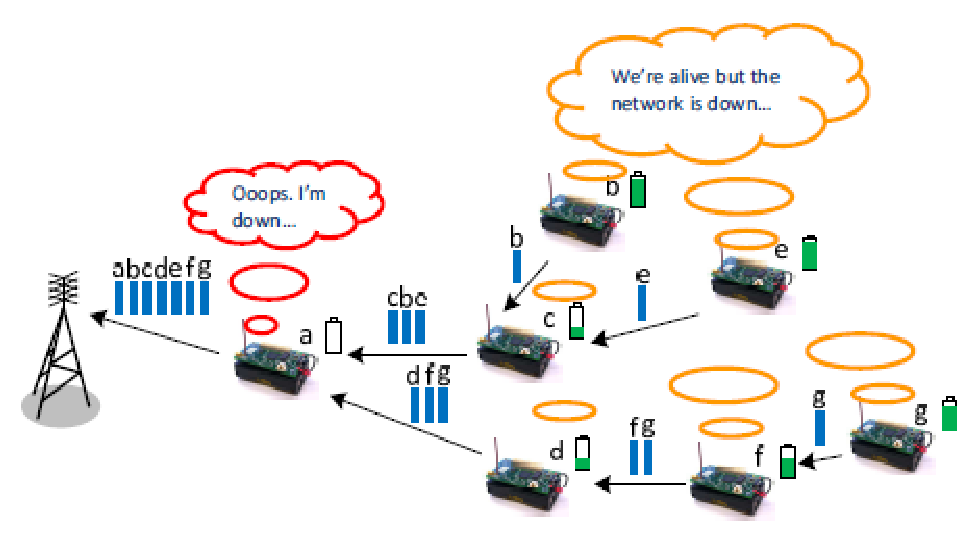
\includegraphics[width=0.8\textwidth]{images/energy_holes.eps}
	\caption{Ένα παράδειγμα υπερφόρτωσης των κόμβων κοντά στην Πηγή}
	\label{fig:energy_holes}
\end{figure}

Λόγω αυτής της υπερφόρτωσης των κόμβων κοντά στην πηγή, οι κόμβοι κοντά στην Πηγή αποφορτίζονται πολύ πιο γρήγορα από ότι οι κόμβοι μακριά από την
Πηγή. Έτσι μετά από μικρό χρονικό διάστημα λειτουργίας του δικτύου οι κόμβοι αυτοί πεθαίνουν και δημιουργούνται μικρές ενεργειακές τρύπες (energy holes). Αυτό
δημιουργεί πρόβλημα στο δίκτυο καθώς αν όλοι οι κόμβοι κοντά στην Πηγή αποφορτιστούν πλήρως, τότε ουσιαστικά το δικτυο καθίσταται άχρηστο καθώς οι κόμβοι που είναι
λίγο πιο μακριά από την Πηγή δεν μπορούν να στείλουν τα δεδομένα τους σε αυτήν. Μάλιστα, έχει δειχθεί οτι σε πρωτόκολλα όπως το Directed Diffusion όταν οι κομβοί
κοντά στην Πηγή πεθάνουν, το δίκτυο έχει ακόμα το 90\% της ενέργειας του \cite{energy_holes}, όπου το μεγαλύτερο μέρος αυτής είναι κατανεμημένο στους κόμβους που
βρίσκονται στην άκρη του δικτύου. Αυτό σημαίνει οτι δεν υπάρχει αποδοτική διαχείρηση της ενέργειας σε αυτά τα πρωτόκολλα. Η λύση σε αυτό το πρόβλημα δίνεται από
αλγόριθμους εξισορρόπησης ενέργειας.

Τα πρωτόκολλα εξισσορόπησης ενέργειας αυτό που προσπαθούν να κάνουν είναι, σε κάθε χρονική στιγμή, όλοι οι κόμβοι του δικτύου να έχουν περίπου την ίδια ενέργεια.
Είναι προφανές οτι τα πρωτόκολλα εξισορρόπησης ενέργειας καταναλώνουν περισσότερη ενέργεια από ότι τα πρωτόκολλα μείωσης της κατανάλωσης ενέργειας. Όμως η διαρκεια
ζωής\footnote{διάρκεια ζωής εννοούμε το χρονικό διάστημα μέχρι το δίκτυο να γίνει άχρηστο.} ενός ΑΔΑ αυξάνεται σημαντικά με τα πρωτόκολλα εξισορρόπησης ενέργειας
αφού σχεδόν όλοι οι κόμβοι είναι ενεργοί καθόλη τη διάρκεια της ζωής του δικτύου ενώ πεθαίνουν όλοι σχεδόν ταυτόχρονα προς το τέλος της. Υπάρχει πoλύ μεγάλη έρευνα
για την εξισορρόπηση ενέργειας στα ασύρματα δίκτυα αισθητήρων ακόμα και σήμερα. Τα πιο σημαντικά πρωτόκολλα
εξισορρόπησης ενέργειας παρουσιάζονται παρακάτω:

\paragraph{EBP:} Το πρωτόκολλο EBP (Energy Balanced Protocol) \cite{ebp_protocol} είναι από τα πρώτα πρωτόκολλα εξισορρόπησης ενέργειας το οποίο έθεσε τις βάσεις του
προβλήματος και πρότεινε έναν πιθανοτικό αλγόριθμο. Συγκεκριμένα, το δίκτυο χωρίζεται σε $n$ δακτύλιους (ή τομείς), πλάτους $R$ ενώ η γωνία που καλύπτει το δίκτυο
θεωρείται οτι είναι $\phi$ οπως φαίνεται στην εικόνα \ref{fig:ebp_ring}.

\begin{figure}[h]
	\centering
	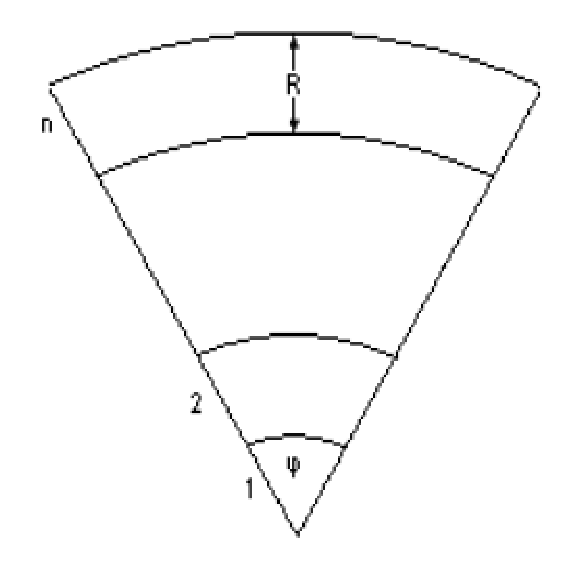
\includegraphics[width=0.4\textwidth]{images/ebp_ring.eps}
	\caption{Δίκτυο αισθητήρων με $n$ δακτυλίδια, γωνία $\phi$ και πλάτος δακτύλιου $R$}
	\label{fig:ebp_ring}
\end{figure}

Για την μετάδοση των πακέτων κάθε κόμβος στον δακτύλιο $i$ χρησιμοποιείται το εξής σχήμα:
\begin{itemize}
\item Μετάδοσε το πακέτο στον δακτύλιο $i-1$ με πιθανότητα $p_{i}$
\item Μετάδοσε το πακέτο απευθείας στην πηγή με πιθανότητα $1-p_{i}$
\end{itemize}

Η επιλογή του $p_{i}$ γίνεται με τέτοιο τρόπο ώστε η μέση κατανάλωση ενέργειας κόμβου να είναι ίδια για όλους τους κόμβους στο δίκτυο.
Μετά από μία εκτενή ανάλυση οι συγγραφείς καταλήγουν στον παρακάτω τύπο:
\begin{align*}
p_{i} = \frac{E[f_{i}]}{E[f_{i+1}] + E[g_{i+1}]}
\end{align*}
όπου $E[f_{i}]$ είναι η μέση τιμή των μηνυμάτων που προωθούνται στον δακτύλιο $i$ και
\begin{align*}
E[f_{i}] = - \sum\limits^{n-i}_{k=1}\frac{\prod_{j=k}^{n-i+1}\alpha(n-j)}{\prod_{j=k}^{n-i}d(n-j)}\cdot
\left(\sum\limits_{j=1}^{n-k}(a(j)E[g_{j}]-\alpha(j+1)E[g_{j+1}])+\alpha(1)\cdot E[f_{1}]\right)
\end{align*}
ενώ $E[g_{i}]$ η μέση τιμή των μηνυμάτων που παράγονται και καθορίζονται από το δίκτυο.

Κάνοντας την παραδοχή οτι $E[f_{i}] \approx E[f_{i+1}]$, οτι δηλαδή τα μηνύματα που προωθούνται στον δακτύλιο $i$ είναι περίπου ίσα με τα μηνύματα που προωθούνται
στον δακτύλιο $i+1$ τότε δημιουργείται ο εξής κλειστός προσεγγιστικός τύπος για τις πιθανότητες $p_{i}$:
\begin{align*}
p_{i} = \frac{3x}{(i+1)(i-1)}
\end{align*}
όπου $p_{2} = x \in (0,1)$ είναι παραμετροποιήσιμη μεταβλητή ενώ $p_{1} =0$.

Όταν το $i$ είναι μεγάλο τότε και η πιθανότητα $p_{i}$ είναι μεγάλη. Αυτό συμβαίνει γιατί όταν ένας κόμβος είναι μακριά από το sink τότε είναι
καλύτερα να στέλνει hop by hop για να αποφύγει να σπαταλήσει μεγάλη ενέργεια για την αποστολή απευθείας στην Πηγή. Αντίθετα, όταν το $i$ είναι μικρό τότε η
πιθανότητα $p_{i}$ είναι μικρή.

\paragraph{Distributed EBP} Η εργασία στο \cite{debp_protocol} είναι μια επέκταση του πρωτοκόλλου EBP. Αρχικά
ορίζεται ως μικτή στρατιγική την δυνατότητα κάθε κόμβου να μπορεί να στείλει είτε στον αμέσως επόμενο γείτονά του είστε απευθείας στην πηγή όπως στο EBP.
Αποδεικνύεται οτι οι μικτές στρατηγικές είναι οι βέλτιστες σε σχέση με οποιαδήποτε άλλη στρατηγική μετάδοσης των πακέτων. Στην συνέχεια κατασκευάζεται ένα τυφλό
άμεσης απόκρισης κατανεμημένο αλγόριθμο (blind, online distributed algorithm) ο οποίος λύνει το πρόβλημα της εξισορρόπησης της ενέργειας. Ο αλγόριθμος λειτουργεί ως
εξής:
\begin{itemize}
\item Αρχικά κάθε κόμβος ξέρει όλους τους γείτονές του και την εναπομείνουσα ενέργειά τους
\item Κάθε κόμβος που θέλει να στείλει ένα πακέτο βρίσκει τον γείτονα με την χαμηλότερη εναπομείνουσα ενέργεια έστω $n_{l}$
	\begin{itemize}
	\item Αν η εναπομείνουσα ενέργεια του $n_{l}$ είναι μεγαλύτερη από την εναπομείνουσα ενέργεια του κόμβου που θέλεί να στείλει το πακέτο τότε το στέλνει στον
$n_{l}$
	\item Αντίθετα αν η εναπομείνουσα ενέργεια του $n_{l}$ είναι μικρότερη τότε ο κόμβος που θέλει να στείλει το πακέτο το στέλνει απευθείας στην πηγή
	\end{itemize}
\end{itemize}

Όπως φαίνεται ο αλγόριθμος χρησιμοποιεί μικτή στρατιγική όπως ο EBP, αλλά είναι κατανεμημένος και χρησιμοποιεί μόνο τοπική πληροφορία, σε αντίθεση με τον EBP.
Εξομοιώσεις δείξαν οτι ο αλγόριθμος μπορεί να εξισορροπήσει σχεδόν τέλεια την ενέργεια σε ένα ασύρματο δίκτυο αισθητήρων.

\paragraph{Offline EBP} H εργασίες στα \cite{oebp_protocol1} και \cite{oebp_protocol2} προσπαθουν να λύσουν το πρόβλημα της εξισορρόπησης ενέργειας από μια
διαφορετική σκοπιά. Η πρώτη εργασία εξετάζει την περίπτωση ομοιόμορφης κατανομής των κόμβων σε ένα δίκτυο το οποίο είναι χωρισμένο σε δακτυλίους όταν ο κάθε κόμβος
στέλνει σχεδόν τον ίδιο αριθμό πακέτων στην Πηγή. Αρχικά αποδεικνύεται οτι για να μειωθεί στο ελάχιστο η κατανάλωση της ενέργειας, οι δακτύλιοι θα πρέπει να έχουν το
ίδιο πλάτος. Όμως με αυτόν τον τρόπο δημιουργείται ανισόρροπη κατανομή ενέργειας στο δίκτυο. Αντίθετα, αποδεικνύεται, οτι για να υπάρχει εξισορρόπηση ενέργειας, το
πλάτος των δακτυλίων μικραίνει όσο είναι πιο κοντά στην πηγή. Στην δεύτερη εργασία μελετάται το ίδιο πρόβλημα όταν υπάρχει μη ομοιόμορφη κατανομή των κόμβων μέσα στο
δίκτυο. Αποδυκνύεται οτι η ανομοιόμορφη κατανάλωση ενέργειας είναι μη αναπόφευκτη σε τέτοια είδη δικτύου. Οι συγγραφείς προτείνουν μία υποβέλτιστη λύση στην οποία ο
αριθμός των κόμβων αυξάνεται με γεωμετρικό ρυθμό από τος έξωτερικούς δακτυλίους προς του εσωετρικούς.


\section{Πρωτόκολλα Δρομολόγησης με Κινητούς Κόμβους}
Πρόσφατη έρευνα έχει δείξει οτι μπορεί να υπάρξει σημαντική μείωση στην κατανάλωση της ενέργειας αν μέσα στο δίκτυο αισθητήρων υπάρχουν μικρές μηχανικά κινητές
συσκευές, ή κινητή κόμβοι, οι οποίες είναι ικανές να μεταφέρουν δεδομένα από ένα σημείο σε ένα άλλο με μηχανική ενέργεια. Για παράδειγμα ένας κινητός κόμβος ο οποίος
μπορεί να μετακινείται μέσα σε όλο την περιοχή του δικτύου, πλησιάζει τους κόμβους αρκετά κοντά προκειμένου οι τελευταίοι να του στείλουν τα δεδομένα τους χωρίς
ιδιαίτερο κόστος. Στην συνέχεια, ο κινητός κόμβος συνεχίζει την πορεία του πλησιάζοντας και άλλους κόμβους για τον ίδιο λόγο. Ανά τακτά χρονικά διαστήματα, ο
κινητός κόμβος, επιστρέφει στην Πηγή πρεοκειμένου να παραδώσει τα δεδομένα του. Πιο ισχυρά μοντέλα υποθέτουν οτι ο κόμβος μπορεί να αποστείλει τα δεδομένα που κατέχει
στην Πηγή από οποιοδήποτε σημείο του δικτύου και αν βρίσκεται. Άλλα μοντέλα θεωρούν οτι η ίδια η πηγή είναι ο κινητός κόμβος. Επίσης στα περισσότερα μοντέλα, η
ενέργεια που καταναλώνει ο κινητός κόμβος κατα την κίνησή του δεν εξετάζεται και θεωρείται αμεληταία.

Ωστόσο, αυτή η αρχιτεκτονική σε κάποια ΑΔΑ μπορεί να δημιουργήσει προβλήματα, κυρίως θέματα χρονοκαθυστέρησης(delay). Για παράδειγμα, μια τυπική ταχύτητα για πολλούς
κινητούς κόμβους (για παράδειγμα το NIMs \cite{nims_mobile}, το Packbot\cite{dynamic_deadlines} και το Robomore\cite{robomore_mobile}) είναι περίπου $0.1-1m/s$.
Επομένως, θα χρειαστεί περίπου 15 λεπτά για μια κινητή συσκευή να διανύσει $1Km$ για να μαζέψει τις πληροφορίες. Τέτοιο χρόνοι είναι απαγορευτικοί για μερικά δίκτυα
αισθητήρων τα οποία απαιτούν πραγματικού χρόνου συλλογή δεδομένων. Σε μερικές εφαρμογές ΑΔΑ όπως είναι η διαχείρηση καταστροφών οι κινητοί κόμβοι θα μπορούσαν να
μεταφερθούν και από μη επανδρωμένα μικρά αεροσκάφη \cite{uav_mobile}. Οι τύποι των διαδρομών που ακολουθούν οι κινητοί κόμβοι μπορούν να ταξινομηθούν στις εξής 3
κατηγορίες:

\begin{itemize}
\item \textbf{Τυχαία κίνηση:} Μπορεί να επιτευχθεί όταν για παράδειγμα οι κόμβοι ενσωματωθούν σε ανθρώπους ή σε ζώα \cite{zebranet}. Γενικώς οι τυχαίοι περίπατοι
(random walks) έχει παρατηρηθεί οτι έχουν ούτε καλή αλλά ούτε κακή απόδοση, είναι όμως πάρα πολύ εύκολο να υλοποιηθούν.

\item \textbf{Ντετερμινιστική κίνηση:} Είδος κίνησης η τροχιά της οποίας είναι προδιαγεγραμμένη από την έναρξη λειτουργίας του δικτύου, όπως είναι ο κύκλος ή η
σπείρα. Οι ιδιότητες της κίνησης, όπως π.χ. ακτίνα, εξάγονται από το ίδιο το δίκτυο. Τέτοιες κινήσεις μπορούν να επιτευχθούν όταν για παράδειγμα οι κόμβοι
ενσωματωθούν σε ένα λεωφορείο το οποίο κάνει συνεχώς την ίδια διαδρομή. Το πλεονέκτημα αυτής της κίνησης είναι οτι αν είναι γνωστή στους στατικούς κόμβους, αυτοί
μπορούν να "ξυπνήσουν" την κατάλληλη στιγμή ωστε να στείλουν τα δεδομένα τους στον κινητό κόμβο.

\item \textbf{Προσαρμοστική κίνηση:} Αυτή η κίνηση εφαρμόζει τεχνικές αλγορίθμων μάθησης και τροποποιείται κατάλληλα ώστε να ανταποκρίνεται κάθε στιγμή στις
απαιτήσεις του δικτύου. Για παράδειγμα σε αν ένα σημείο του δικτύου υπάρχει πολύ μεγάλος ρυθμός παραγωγής γεγονότων, τότε ο κινητός κόμβος κάθεται για περισσότερο
διάστημα σε αυτό το σημείο ώστε να ξεκουράσει τους γύρω κόμβους.

\item \textbf{Ελεγχόμενη κίνηση:} Όταν ο κιητός κόμβος ενσωματωθεί σε ένα τηλεκατευθυνόμενο robot ή αεροπλάνο (UAV) τότε η κατεύθυνση και η ταχύτητα μπορεί να
τροποποιηθεί κάθε στιγμή από τον ίδιο τον άνθρωπο. Συνήθως τέτοιες κινήσεις δεν αναλύονται στα μοντέλα ΑΔΑ.
\end{itemize}



Γενικώς η κίνηση (είτε είναι κινητή Πηγή είτε κινητός κόμβος είτε πολλοί κινητοί κόμβοι) στα σύρματα δίκτυα αισθητήρων χρησιμοποιείται εξής λόγους:

\begin{itemize}
\item \textbf{Βελτίωση της κάλυψης του δικτύου:} Οι κόμβοι συνήθως αναπτύσσονται τυχαία μέσα στην περιοχή ανίχνευσης είτε από τον αέρα (π.χ. από ένα
αεροπλάνο/ελικόπτερο) είτε από ένα ρομπότ. Όμως ακόμα και αν θεωρηθεί οτι οι κόμβοι αναπτύσσονται ομοιόμορφα κατανεμημένα, αυτό δεν μπορεί να εγγυηθεί οτι δεν θα
υπάρχουν τοπικά μέγιστα και ελάχιστα. Επομένως μπορεί σε κάποιο σημείο του δικτύου να μην καλύπτεται επαρκώς από τους ήδη υπάρχοντες κόμβους. Ένας κινητός κόμβος
μπορεί να πάει σε αυτή τη θέση και να προσομοιώσει έναν στατικό κόμβο προκειμένου να καλυφθεί πλήρως η περιοχή ανίχνευσης.
\item \textbf{Βελτίωση της συνδεσιμότητας του δικτύου:} Οι κινητοί κόμβοι μπορούν να προσφέρουν ένα μονοπάτι ανάμεσα σε δύο συνεκτικές συνιστώσες του δικτύου. Για
παράδειγμα μπορεί μερικοί κρίσιμοι κόμβοι να πάθουν βλαβη και επομένως το δίκτυο να "κοπεί" ουσιαστικά στη μέση. Οι κινητοί κόμβοι μπορούν να αποτρέψουν ένα τέτοιο
γεγονός.
\item \textbf{Μεταφορά δεδομένων από απομακρυσμένους κόμβους:} Μερικοί κόμβοι σε ένα ασύρματο δίκτυο αισθητήρων μπορεί να μην έχουν συνδεσιμότητα με κανέναν άλλο
κόμβο και επομένως να μην μπορούν να μεταδώσουν τα δεδομένα τους στην Πηγή. Αυτό μπορεί να επιτευχθεί αν ένας κινητός κόμβος προσεγγίσει τους απομακρυσμένους κόμβους
της πηγής και λάβει τα αποθηκευμενα δεδομένα των κόμβων αυτών και τα μεταφέρει σε άλλους κόμβους ή στην Πηγή.
\item \textbf{Αύξηση του χρόνου ζωής του δικτύου:} Αποτελεί από τους πιο σημαντικούς λόγους που χρησιμοποιείται η κίνηση στα δίκτυα αισθητήρων. Οι κινητοί κόμβοι
μπορούν να προσεγγίσουν περιοχές στις οποίες υπάρχουν ενεργά μονοπάτια μεταφοράς δεδομένων και να βοηθήσουν αυτούς τους κόμβους μεταφέροντας οι ίδιοι τα δεδομένα
μηχνανικά.
\begin{figure}[h]
	\centering
	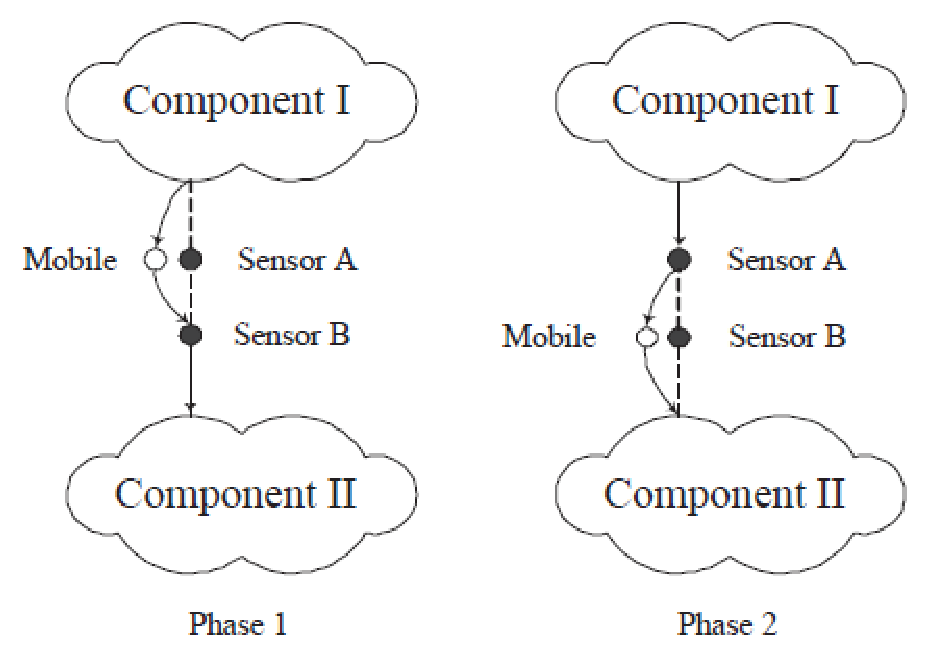
\includegraphics[width=0.6\textwidth]{images/mobile_help.eps}
	\caption{O κινητός κόμβος βοηθάει τους υπερφορτωμένους στατικούς κόμβους.}
	\label{fig:mobile_help}
\end{figure}
Ενα τέτοιο παράδειγμα φαίνεται στην εικόνα \ref{fig:mobile_help} (εξαγμένη από το \cite{using_mobile_elements_to_prolong_lefetime}). Ολόκληρο το δίκτυο αποτελείται
από δύο μικρότερα υποδύκτια ( Compnent I \& II) τα οποία είναι συνδεδεμένα μέσω των κόμβων Α και Β. Επομένως οι δύο αυτοί κόμβοι αποτελούν πέρασμα συμφώρησης αφού
πρέπει να προωθούν όλη την κίνηση από τα 2 υποδίκτυα. Ένας κινητός κόμβος μπορεί να προσομοιώσει την λειτουργία των Α και Β και έτσι να βελτιώσει τον χρόνο ζωής των
κόμβων αυτών και κατα συνέπεια του συνολικού δικτύου. Επίσης οι κινητοί κόμβοι μπορούν να συλλέξουν τα δεδομένα των στατικών κόμβων μέσω μικρής ακτίνα μετάδοσης
βοηθώντας στην εξοικονόμηση ενέργειας του κάθε κόμβου ξεχωιριστά. Συγκεκριμένα, προκειμένου να μεγιστοποιηθεί ο χρόνος ζωής στο δίκτυο, ο κάθε στατικός κόμβος θα
πρέπει να στέλνει τα δεδομένα του σε έναν κινητό κόμβο αν και μόνο αν αυτός είναι σε απόσταση μικρότερης του ενός βήματος (hop). Ωστόσο, με αυτόν τον τρόπο υπάρχει
πολύ μεγάλη χρονοκαθυστέρηση (delay) στην μεταφορά των δεδομένων στην Πηγή. Από την άλλη μεριά αποστέλοντας απ'ευθείας στην Πηγή ή χρησιμοποιώντας multi-hop
πρωτόκολλα για την άμεση αναφορά γεγονότων στην Πηγή μειώνει δραστικά την χρονοκαθυστέρηση αλλά και τον χρόνο ζωής του δικτύου. Επομένως απαιτείται μία χρυσή τομή
ανάμεσα στην χρονοκαθυστέρηση και τον χρόνο ζωής του δικτύου που σίγουρα εξαρτάται από τον σκοπό και το περιβάλλον του δικτύου αισθητήρων.
\end{itemize}

Στη βιβλιογραφία έχουν χρησιμοποιηθεί πολλές διαφορετικές έννοιες για την περιγραφή των κινητών κόμβων στα ασύρματα δίκτυα αισθητήρων. Οι όροι διαφέρουν μεταξύ τους
ως προς το είδος και τον σκοπό του κινητού κόμβου. Για παράδειγμα κινητή Πηγή (mobile Sink ή mobile BS) χρησιμοποιείται για να περιγράψει μια κινητή Πηγή η οποία
έχει την δυνατότητα να περισυλλέγει δεδομένα από τους κοντινούς της κόμβους καθώς κινείται προκειμένου αυτοί να κάνουν πιο εικονομικές μεταδόσεις σε σχέση με μία
στατική Πηγή. Παρόμοια ο όρος κινητή οντότητα ή πιο γενικά κινητός κόμβος (mobile MULES, mobile entities, mobile relays) αναφέρεται σε κινητούς κόμβους οι οποίοι
έχουν πρόμοια υπολογιστική ισχύ όπως μια Πηγή και περιφέρονται σε όλο την περιοχή προκειμένου να περισυλλέξουν δεδομένα. Συχνά σε αυτό το μοντέλο είναι οτι
στο ασύρματο δίκτυο υπάρχει και μία Πηγή στην οποία οι κινητοί κόμβοι στέλνουν τα δεδομένα των στατικών κόμβων.

Επειδή η έρευνα σε αυτό τον τομέα των ασύρματων δικτύων αισθητήρων συνεχίζεται ακόμα και υπάρχει μεγάλο ενδιαφέρον στην πλήρη αξιοποίηση των κινητών κόμβων σε ένα
ΑΔΑ, θα παρουσιαστούν παρακάτων οι πιο σημαντικές εργασίες σε σχέση με την εκμετάλευση κινητών Πηγών και κινητών κόμβων σε ένα δίκτυο αισθητήρων.

\subsection{Πρωτόκολλα με Κινητή Πηγή}
Η εργασία στο \cite{jointmobility} εξετάζει αν η κίνηση και η δρομολόγηση σε ένα δίκτυο αισθητήρων είναι φιλικές ή αλληλοσυγκρουόμενες έννοιες. Στο μοντέλο τους
εξετάζουν την περίπτωση ενός πυκνού δικτύου στο οποίο υπάρχουν στατικοί κόμβοι, τοποθετημένοι με μια Poisson κατανομή σε έναν κύκλο, έχουν μικρή ενέργεια και μια
κινητή Πηγή με άπειρη ενέργεια περιφέρεται στο δίκτυο προκειμένου να βοηθήσει στην δρομολόγηση και να περισυλλέξει τα δεδομένα όπως φαίνεται στην εικόνα
\ref{fig:jointmobility_model}.
\begin{figure}[h]
	\centering
	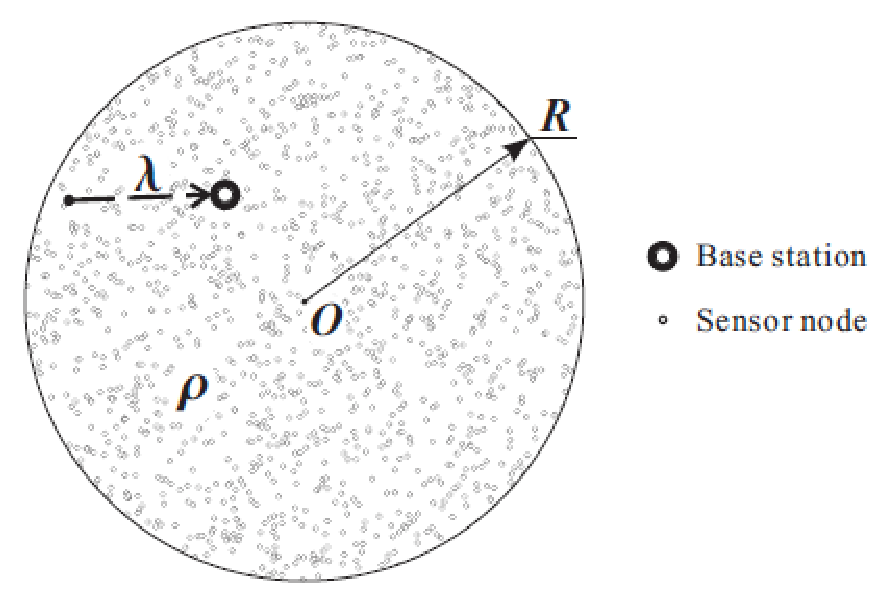
\includegraphics[width=0.6\textwidth]{images/jointmobility_model.eps}
	\caption{Κόμβοι τοποθετημένοι με Poisson κατανομή και Πηγή να κινειται στην περιφέρεια του κύκλου.}
	\label{fig:jointmobility_model}
\end{figure}
Οι συγγραφείς εξετάζουν την βέλτιστη θέση της Πηγής όταν αυτή είναι στατική και την βέλτιστη διαδρομή όταν αυτή είναι κινητή. Τελικά αποδεικνύουν οτι η βέλτιστη θέση
για την Πηγή όταν αυτή είναι στατική είναι το κέντρο του κύκλου. Αντίθετα όταν η Πηγή είναι κινητή αποδεικνύουν οτι η βέλτιστη διαδρομή της Πηγής είναι η περιφέρεια
του κύκλου. Αυτό συμβαίνει γιατί η διαδρομή αυτή είναι η μεγαλύτερη δυνατή που υπακούει και στην γεωμετρία του μοντέλου. Μια σύγκριση της εναπομείνουσας ενέργειας με
τα προαναφερθέντα μοντέλα φαίνονται στην εικόνα \ref{fig:jointmobility_dissipation}.
\begin{figure}[h]
	\centering
	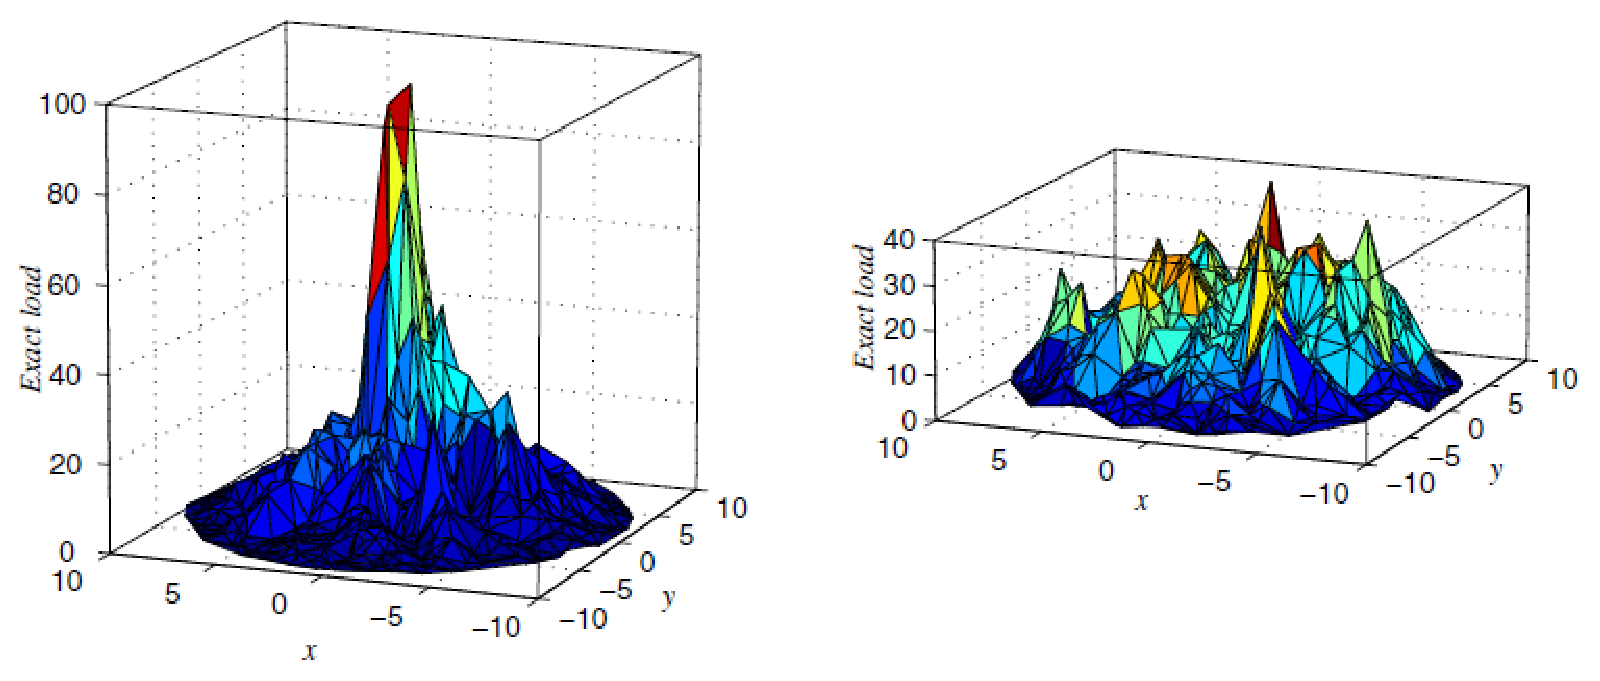
\includegraphics[width=\textwidth]{images/jointmobility_dissipation.eps}
	\caption{Ο ρυθμός κατανάλωσης της ενέργειας όταν η Πηγή είναι στο κέντρο του δικτύου(δεξιά) και όταν η κινείται στην περιφέρειά του(αριστερά).}
	\label{fig:jointmobility_dissipation}
\end{figure}

Όπως φαίνεται στην πρώτη εικόνα η στατική πηγή δημιουργεί στους γύρω της κόμβους πολύ μεγάλους ρυθμούς κατανάλωσης ενέργειας. Αντίθετα, όταν η Πηγή είναι κινητή και
κινείται στην περιφέρεια του κύκλου, υπάρχει μεγαλύτερη εξισσορόπηση ενέργειας στο δίκτυο και επομένως αυξάνεται ο χρόνος ζωής του.
\begin{comment}
edw den einai pio logiko h phgh na kineitai kapou sto endiameso ths aktinas R kai pio sugkekrimena otan ta 2 emvada ginoun isa ? prepei na to melethsw....
\end{comment}

Οι συγγραφείς παρουσίασαν μια ακόμη εργασία στο \cite{jointmobility_2006} ως συνέχεια της προηγούμενης στην οποία το μοντέλο με την προηγούμενη
εργασία και συγκρίνουν 2 περιπτώσεις για την αύξηση του χρόνου ζωής του δικτύου.
\begin{itemize}
\item \textbf{Γρήγορη κίνηση της Πηγής:} εξισσορόπηση της χρονοκαθυστέρησης (delay) με την κατανάλωση της ενέργειας
\item \textbf{Αργή κίνηση της Πηγής:} παροχή βοήθειας στους κρίσιμους κόμβους (bottleneck nodes)
\end{itemize}
Η αργή κίνηση της Πηγής επιτυγχάνεται μέσα από ένα γραμμικό πρόγραμμα
\begin{align*}
\text{Maximizing network lifetime } & T=\sum\limits_{i}T_{i}\\
\text{Constraints } & \sum\limits_{i}T_{i}P_{i}\leq E
\end{align*}
όπου $Τ_{i}$ ο χρόνος ζωής κάθε κόμβου, $P_{i}$ ο ρυθμός κατανάλωσης ενέργειας του κάθε κόμβου ως προς τον χρόνο και $E$ η συνολική ενέργεια του δικτύου.
Στην εργασία προτείνεται ένας αλγόριθμος 2 φάσεων ο οποίος χρησιμοποιεί το παραπάνω γραμμικό πρόγραμμα
\begin{itemize}
\item \textbf{Αρχικοποίηση:} Κατα την αρχικοποίηση η κινιτή Πηγή επισκέπτεται όλους τα σημεία-σταθμούς, συλλέγει τον ρυθμό κατανάλωσης κάθε σταθμού και κατασκευάζει
ένα προφίλ αυτού του σημείου-σταθμούς
\item \textbf{Εν λειτουργία:} Κατα την πραγματική λειτουργία η κινητή Πηγή παραμένει σε κάθε σημείο-σταθμό χρονικό διάστημα ανάλογο με τον ρυθμό κατανάλωσης ενέργειά
του.
\end{itemize}
Τα πειράματα αυτής της εργασίας έδειξαν οτι υπάρχει σημαντική αύξηση του χρόνου ζωής με τον αλγόριθμο των 2 φάσεων. Όμως ο αλγόριθμος δεν μπορεί να είναι
αποδοτικός και να επεκταθεί σε πολύ μεγάλα δίκτυα καθώς υπάρχει σημαντική καθυστέρηση.


Στην εργασία \cite{marios_randomwalks_1} αναλύεται η περίπτωση που υπάρχει κινητή Πηγή και αυτή κάνει έναν τυχαίο περίπατο (random walk). Γενικώς οι τυχαίοι
περίπατοι είναι πολύ εύκολοι στην υλοποίηση αφού χρησιμοποιούν μόνο τοπικές πληροφορίες και μπορούν να μειώσουν σημαντικά την κατανάλωση της ενέργειας λόγω της
τυχαιότητάς τους. Οι συγγραφείς προκειμένου να κάνουν ακόμα πιο αποδοτικούς τους τυχαίους περίπατους, δημιουργούν τους προσαρμοστικούς τυχαίους περίπατους. Σε αυτή
την περίπτωση, η κινητή Πηγή εκμεταλεύεται κάποιες επιπλέον τοπικές πληροφορίες προκειμένου να επηρρεάσει το επόμενο βήμα της, το οποίο και πάλι γίνεται πιθανοτικά
μόνο που αυτή τη φορά όχι τελείως ομοιόμορφα τυχαία αλλά προς την σωστότερη κατεύθυνση. Στο μοντέλο της εργασίας, η περιοχή του δικτύου χωρίζεται σε κελιά στα οποία
μόλις βρεθεί η κινητή Πηγή μέσα σε ένα από αυτά, γνωρίζει την κστάσταση όλων των αισθηρήρων που ανήκουν στο ίδιο κελί. Οι συγγραφείς συγκρίνουν διάφορους τύπους
τυχαίων περιπάτων:
\begin{itemize}
\item \textbf{Τυφλός τυχαίος περίπατος:} Σε αυτή την περίπτωση η κινητή Πηγή επιλέγει ομοιόμορφα τυχαία μία από τις 4 κατευθύνσεις που θα ακολουθήσει στο επόμενο
βήμα. Αν και πιθανοτικά αυτή η λύση εγγυείται οτι η Πηγή θα φθάσει σε όλους τους κόμβους και όλα τα δεδομένα θα περισυλλεγούν, δημιουργεί σημαντικά προβλήματα
χρονοκαθυστέρησης. Για παράδειγμα η κινητή Πηγή μπορεί πολλές φορές να πηγαίνει σε σημεία τα οποία έχει ξαναεπισκεφθεί.
\item \textbf{Τυχαίος περίπατος με μνήμη:} Σε αυτή την περίπτωση η κινητή Πηγή θυμάται τα $Κ$ τελευταία κελιά τα οποία έχει επισκεφθεί κατα την διάρκεια του τυχαίου
περίπατου της. Κάθε φορά το επόμενο βήμα επιλέγεται τυχαία με βάση τα κελιά τα οποία δεν ανήκουν στα $Κ$ τελευταία. Φυσικά ύπάρχει ένας συμβιβασμός (trade off) ως
προς το μέγεθος του $K$. Για παράδειγμα αν το $K$ είναι πολύ μικρό, τότε η κινητή Πηγή ουσιαστικά εκτελεί τυχαίο περίπατο. Αντίθετα αν το $Κ$ είναι πολύ μεγάλο η
κινητή Πηγή μπορεί να βρεθεί σε κάποιο αδιέξοδο όταν για παράδειγμα όλα τα επόμενα δυνατά κελιά τα έχει ήδη επισκεφθεί.
\item \textbf{Τυχαίος περίπατος με αδράνεια:} Στην περίπτωση αυτή η πιθανότητα κάθε κατεύθυνσης του επόμενου βήματος προσαρμόζεται ανάλογα με την ανακάλυψη νέων
κόμβων. Συγκεκριμένα ο αλγόριθμος ενισχύει τις κατευθύνσεις στις οποίες εμφανίζονται καινούργιοι κόμβοι και αποδυναμώνει τις κατευθύνσεις στις οποίες υπάρχουν κόμβοι
που ήδη έχουν επισκεφθει.
\item \textbf{Τυχαίος περίπατος explore n go:} Σε αυτή την περίπτωση η κινητή Πηγή ακολουθεί μία ευθεία γραμμή (δηλαδή προχωράει ίσια) όσο βρίσκει καινούργιους
κόμβους και αλλάζει κατεύθυνση αν βρεθούν κόμβοι που έχουν επισκεφθεί ή φθάσει στην άκρη του δικτύου. Ο τυχαίος περίπατος αυτός έχει παρόμοια απόδοση με τον τυχαίο
περίπατο με αδράνεια.
\item \textbf{Κατσαρός (curly) τυχαίος περίπατος:} Ο τυχαίος περίπατος αυτός παρομοιάζει την ντετερμινιστική σπείρα. Συγκεκριμένα η κινητή Πηγή ξεκινάει από μια
περιοχή και εκτελεί αριστερές στροφές οι οποίες μεγαλώνουν με τον χρόνο. Μετά από αρκετό διάστημα, ο τυχαίος περίπατος θα έχει καλύψει όλο το δίκτυο.
\end{itemize}

Οι προσομοιώσεις έδιξαν οτι οι προσαρμοστικοί τυχαίοι περίπατοι κινητών Πηγών έχουν πολύ καλύτερα αποτελέσματα όσον αφορά την περισυλλογή των δεδομένων από τους
κόμβους σε σχέση με τους τυχαίους περίπατους.

Στην εργασία \cite{deploying_multiple_sinks_wsns} αναλύεται η βέλτιστη τοποθεσία μιας κινητής Πηγής σε πολυ-βηματικά (multi-hop) δίκτυα αισθητήρων. Συγκεκριμένα οι
συγγραφείς αναπτύσουν αρχικά έναν καθολικό αλγόριθμο μέσα από γραμμικό προγραμματισμό. Αποδεικνύουν οτι το βέλτιστο σημείο στο οποίο θα πρέπει να πάει μια κινητή Πηγή
προκειμένου να υπάρχει μείωση της κατανάλωσης της ενέργειας είναι αυτό στο οποίο το άθροισμα όλων των διανυσμάτων κόμβου-Πηγής ισούται με το 0. Ουσιαστικά πρόκειται
για το γεωμετρικό κέντρο. Επειδή ο αλγόριθμος αυτός απαιτεί καθολικά (global) δεδομένα, οι συγγραφείς προτείνουν έναν αλγόριθμο που χρησιμοποιεί τοπικά δεδομένα αλλά
πετυχαίνει σχεδόν το ίδιο αποτέλεσμα με τον καθολικό αλγόριθμο. Στον τοπικό αλγόριθμο, κάθε κόμβος κρατάει στη μνήμη του τον αριθμό των μονοπατιών τα οποία έχουν
δημιουργηθεί από το πρωτόκολλο δρομολόγησης και παιρνάνε από μέσα του. Με αυτόν τον τρόπο η κινητή Πηγή χρειάζεται τα δεδομένα μόνο των πρώτων γειτόνων της οι οποίοι
θα έχουν σίγουρα αριθμό μονοπατιών μεγαλύτερο από τους πιο μακρινούς γείτονές της. Οι αριθμοί αυτοί προσομοιώνουν τα διανύσματα αποστάσεων που αναφέρθηκαν νωρίτερα.
Έτσι, αν ας κόμβος έχει μεγάλο αριθμό μονοπατιών, η πηγή κινείται προς αυτό το σημείο προκειμένου να "ξεκουράσει" τον κόμβο. Στην εργασία αυτή, οι συγγραφείς
μελετάνε και την περίπτωση πολλών κινητών Πηγών.

\subsection{Πρωτόκολλα με Κινητούς Κόμβους} %nikoletsea's paper
Όπως και στην περίπτωση της μιας κινητής Πηγής στο δίκτυο αισθητήρων έτσι και στην περίπτωση πολλών κινητών Πηγών-κόμβων υπάρχει πολύ μεγάλη έρευνα. Αν και σε πολλές
εργασίες απλά επεκτείνεται η λογική της μίας κινητής Πηγής σε πολλές, η σωστή κατανομή των πηγών καθώς και ο σωστός αριθμός των πηγών αποτελούν χαρακτηριστικά προς
έρευνα.

Η εργασία στο \cite{data_mules} αποτελεί σημείο αναφοράς για τα δίκτυα αισθητήρων με κινητούς κόμβους. Στο μοντέλο θεωρείται ένα ΑΔΑ τριών επιπέδων. Στο κάτω επίπεδο
βρίσκονται οι στατικοί κομοι οι οποίοι επιβλέπουν το περιβάλλον. Στο αμέσως απο πάνω επίπεδο βρίσκονται οι κινητοί κόμβοι οι οποίοι επιεκέπτονται τους στατικούς
κόμβους προκειμένου να συλλέξουν πληροφοριές. Τέλος στο ανώτερο επίπεδο βρίσκονται τα σημεία πρόσβασης (ΣΠ ή acces points) τα οποία ουσιαστικά αποτελούν Πηγές στις
οποίες παραδίδονται όλα τα δεδομένα των κινητών κόμβων. Επίσης θεωρείται οτι οι κινητοί κόμβοι θα πρέπει να φτάσουν σε απόσταση ενός βήματος (1-hop) ώστε να μπορούν
να επικοινωνήσουν με άλλους κόμβους ή σημεία πρόσβασης. Για την ανάλυση της απόδοσης, το δίκτυο χωρίζεται σε πλέγματα. Στην συνέχεια αποδεκνύεται οτι για $\rho_{AP}$
η πυκνότητα των σημείων πρόσβασης, η μέση τιμή του χρόνου που χρειάζεται ένας κινητός κόμβος να ξεκινήσει από ένα σημείο πρόσβασης και να ξανακαταλήξει σε αυτό ή σε
ένα άλλο κάνοντας τυχαίο περίπατο είναι $\frac{1}{\rho_{AP}}$. Επίσης, αποδεικνύεται οτι ο μέσος χρόνος που χρειάζεται να συναντήσει ένας κινητός κόμβος έναν τυχαίο
στατικό κόμβο είναι $\rho_{MULES}$ όπου $\rho_{MULES}$ είναι η πυκνότητα των κινητών κόμβων στο δίκτυο. Αντίστοιχα αποτελέσματα αποδεικνύονται για την πρώτη επίσκεψη
(hitting time) και την ποσότητα δεδομένων που αποθηκεύονται στη μνήμη των κόμβων αλλά και τον λόγο επιτυχίας των μηνυμάτων. Φυσικά όλα τα αποτελέσματα αναφέρονται σε
μέσες τιμές και προκειμένου να υπάρχει συγκέντρωση γύρω από την μέση τιμή θα πρέπει να εφαρμοστούν μέθοδοι που βασίζονται σε ροπές δεύτερης τάξης. Ωστόσο, η ανάλυση
που παρουσιάζεται σε αυτή την εργασία αποτελεί ένα καλό βοήθημα για την κατανόηση παρόμοιων μοντέλων.

Στην εργασία \cite{yuanyuan1} αναλύεται το πρόβλημα της τοποθέτησης κινητών κόμβων οι οποίοι θα λειτουργούν ως αρχηγοί σε συστάδες. Στο μοντέλο τους, παρουσιάζουν
μια αρχιτεκτονική τριών επιπέδων στην οποία στη βάση υπάρχουν οι στατικοί κόμβοι, μετά υπάρχουν οι κινητοί κόμβοι και τέλος υπάρχει η Πηγή. Θεωρούν οτι οι
κινητοί κόμβοι μπορούν να επικοινωνήσουν μεταξύ τους και με την Πηγή ώστε να της αποστείλουν τα τελικά δεδομένα. Αφού δείξουν οτι το πρόβλημα τοποθέτησης των κινητών
κόμβων στο δίκτυο ώστε να μεγιστοποιηθεί ο χρόνος ζωής του δικτύου είναι NP-hard (κάνοντάς το αναγωγή στο k-center πρόβλημα) παρουσιάζουν έναν ευρετικό αλγόριθμο που
λύνει το πρόβλημα αυτό σχετικά γρήγορα. Ο ευρετικός αλγόριθμος βασίζεται στην κατασκευή ενός χάρτη των ενεργειών των κόμβων της συστάδας μέσα από πληροφορίες των κόμ
ων της ίδιας της συστάδας.


Η εργασία στο \cite{event_residual_hybrid} ακολουθεί μοντέλο παρόμοιο με την προηγούμενη. Οι συγγραφείς αναλύουν αρχικά από τι εξαρτάται ο χρόνος
ζωής ενός δικτύου και στην συνέχεια βασιζόμενοι στην ανάλυσή τους προτείνουν έναν υβριδικό αλγόριθμο. Οπως αποδεικνύουν ο χρόνος του δικτύου εξαρτάται απο πολλούς
παράγοντες, οι πιο σημαντικοί από τους οποίους είναι: από την αρχική του ενέργεια, τον ρυθμό που παράγονται οι πληροφορίες, το μέγεθος του δικτύου, την ακτίνα
μετάδοσης ενός κόμβου αλλά και ενεργειακοί παράγοντες που αφορούν τα κυκλώματα του κάθε κόμβου για την λειτουργία των κυκλωμάτων. Παρουσιάζουν 2 στρατηγικές για τις
κινητές Πηγές που μπορούν να υπάρξουν. Στην πρώτη η κάθε κινητή Πηγή πηγαίνει στο σημείο μικρότερης ενέργειας της συστάδας της. Το πλεονέκτημα αυτής της στρατηγικής
είναι οτι δημιουργείται ένα πλήρως ενεργειακά ομοιόμορφο δίκτυο και επομένως αυξάνεται ο χρόνος ζωής του. Στην δεύτερη στρατηγική η κάθε κινητή Πηγή πηγαίνει ακριβώς
στο σημείο που παράγεται ένα γεγονός. Σε αυτή την περίπτωση η κινητή Πηγή λαμβάνει άμεσα τα δεδομένα από το γεγονός, το οποίο στο μοντέλο διαρκεί αρκετό χρονικό
διάστημα, έτσι ώστε τα δεδομένα δεν στέλνονται στους υπόλοιπους κόμβους και επομένως χάνεται ελάχιστη ενέργεια για την μεταφορά αυτών. Όμως η στρατηγική αυτή
δημιουργεί ανομοιογενή κατανομή ενέργειας στο δίκτυο. Ο υβριδικός αλγόριθμος που παρουσιάζουν οι συγγραφείς συνενώνει τις 2 στρατηγικές. Πειράματα έδειξαν
σημαντική βελτίωση του χρόνου ζωής του δικτύου.

Η εργασία στο \cite{yuanyuan2} αναλύεται ξανά η βέλτιστη τοποθέτηση των κινητών Πηγών οι οποίες λειτουργούν ως αρχηγοί συστάδων όπως στο \cite{yuanyuan1} αλλά αυτή
τη φορά οι συγγραφείς στοχεύουν στην αποδοτική περισυλλογή δεδομένων. Αφού αποδείξουν οτι το πρόβλημα αυτό είναι NP-hard με αναγωγή στο TSP πρόβλημα παρουσιάζουν τον
αλγόριθμό τους ο οποός αποτελείται απο 3 βήματα και παρουσιάζεται στην εικόνα \ref{fig:yuanyuan_mst}.
\begin{figure}[h]
	\centering
	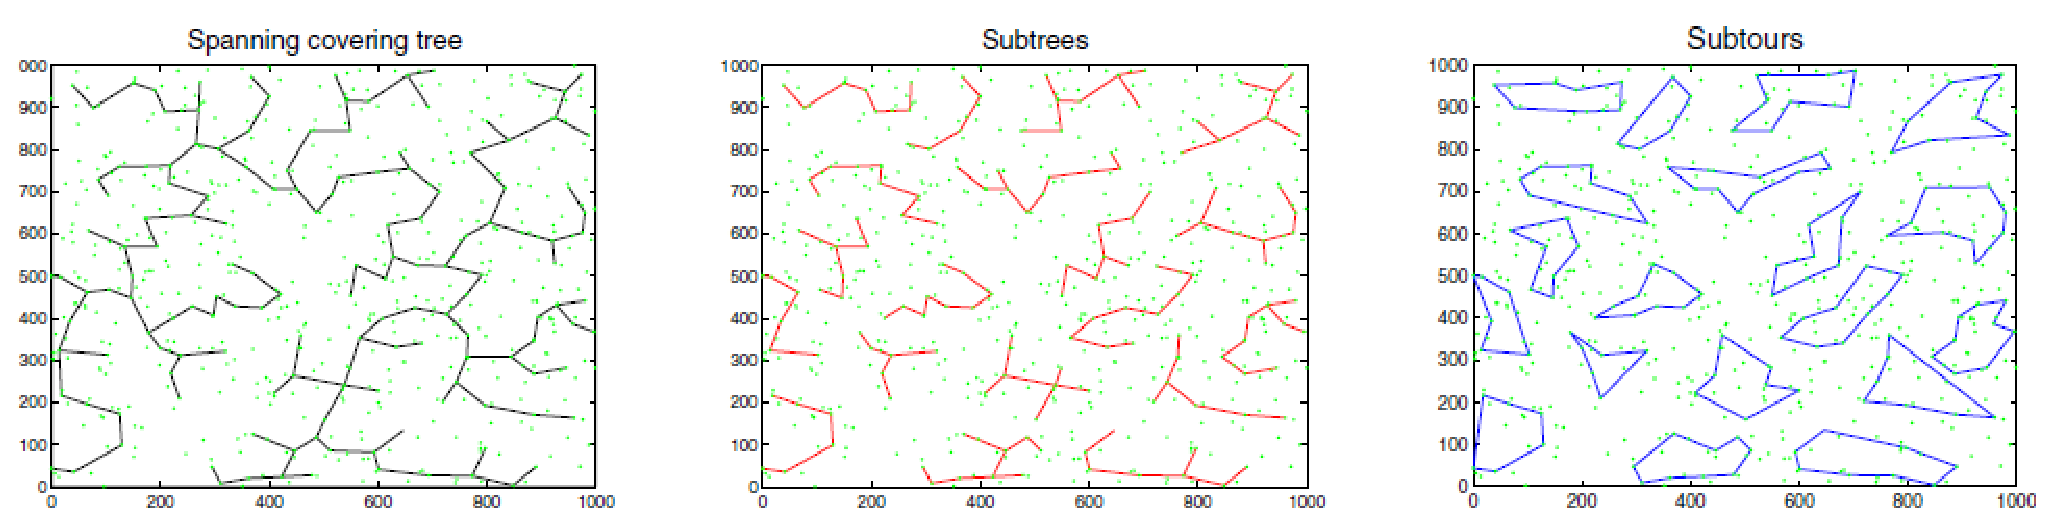
\includegraphics[width=\textwidth]{images/yuanyuan_mst.eps}
	\caption{Τα 3 βήματα του αλγορίθμου.}
	\label{fig:yuanyuan_mst}
\end{figure}
Αρχικά κατασκευάζεται κατανεμημένα ένα ελάχιστο γεννητικό δέντρο με όλους τους κόμβους, το δέντρο αυτό αποσυντίθεται σε μικρότερα ελάχιστα γεννητικά δέντρα, όσες και
οι κινητές Πηγές και αναζητείται σε κάθε τέτοιο δέοντρο το μικρότερο μονοπάτι το οποίο επιεκέπτεται όλους τους κόμβους. Οι κινητές Πηγές στέλνουν τα δεδομένα τους
στην κύρια Πηγή χρησιμοποιώντας της υπόλοιπες κινητές Πηγές. Πειράματα έδιξαν οτι εξοικονομείται σημαντικό ποσό της ενέργειας.


Η εργασία στο \cite{dynamic_deadlines} εξετάζει το πρόβλημα από μια διαφορετική σκοπιά. Οι συγγραφείς αρχικά επισημένουν οτι το πρόβλημα με τις κινητές Πηγές
ουσιαστικά πρόκειται για την δρομολόγηση κινητών με χρονικές προθεσμίες οι οποίες καθορίζονται από τον χώρο μνήμης ενός κόμβου ή πιο αφαιρετικά από το μέγιστο μέγεθος
των δεδομένων κάθε κόμβου θα κρατάει πριν τα παραδώσει στην Πηγή. Υπο αυτή την έννοια το πρόβλημα είναι λίγο διαφορετικό από το TSP πρόβλημα με την έννοια οτι η κάθε
κινητή Πηγή μπορεί να χρειαστεί να επισκεφθεί περισσότερες από μια φορά έναν κόμβο ανάλογα με τον ρυθμό παραγωγής των γεγονότων σε εκείνη την περιοχή. Αφού
αποδείξουν οτι το πρόβλημα είναι NP-complete κατασκευάζουν 3 ευρετικούς αλγορίθμους.
\begin{itemize}
\item \textbf{Νωρίτερη προθεσμία πρώτα:} σε αυτή την περίπτωση ο αλγόριθμος επισκέπτεται πρώτα τον κόμβο του οποίου ο χώρος μνήμης είναι πιο κοντά να ξεχειλείσει. το
πρόβλημα με αυτόν τον ευρετικό αλγόριθμο είναι οτι δεν παίρνει υπόψην του καθόλου το κόστος του κάθε κόμβου για να τον επισκεφθεί, δηλαδή την απόστασή του από την
τωρινή θέση της κινητής Πηγής.
\item \textbf{Νωρίτερη προθεσμία με $k$-κόμβους μπροστά:} σε αυτή την περίπτωση η κινητή Πηγή ταξινομεί τις προθεσμίες όλων των κόμβων και επιλέγει τις $k$
μικρότερες. Στη συνέχεια, επιλέγει την σειρά με την οποία θα επισκεφθεί τους $k$ αυτούς κόμβους έτσι ώστε καμία προθεσμία να μην χαθεί και ταυτόχρονα η συνολική
διαδρομή, δηλαδή ο χρόνος που θα χρειαστεί, να είναι η μικρότερη δυνατή.
\item \textbf{Ελάχιστο ζυγισμένο άθροισμα πρώτα:} σε μία προσπάθεια να εξισορροπήσουν το κόστος απόστασης με την χρονική προθεσμία οι συγγραφείς δημιούργησαν αυτόν
τον υβριδικό ευρετικό αλγόριθμος. Δηλαδή δημιουργούν το διάνυσμα
\begin{align*}
weighted\_sum[i] = & \alpha_{mwsf}\dot (deadline[i]-current\_time[i]) +\\
& (1-\alpha_{mwsf})(cost[current\_position][i])
\end{align*} και επιλέγουν τον κόμβο που έχει την μικρότερη τιμή.
\end{itemize}
Στην συνέχεια συγκρίνουν τους αλγορίθμους αυτούς με έναν αρκετά γνωστό
ευρετικό αλγόριθμο ο οποίος προέρχεται από την δρομολόγηση οχημάτων \cite{vehicle_routing_windows}. Τα βήματα του αλγορίθμου είναι τα εξής:
\begin{enumerate}
\item Ξεκινάει με ένα όχημα και έναν κόμβο ο οποίος είναι ο πρώτος στην διαδρομή του
\item Στην συνέχεια βρίσκει τον καλύτερο κόμβο που μπορεί να εισέλθει στην διαδρομή του
\begin{itemize}
	\item Αυτό συνεχίζεται μέχρι κανένας νέος κόμβος να μην μπορεί να εισέλθει λόγω περιορισμών στις προθεσμίες
\end{itemize}
\item Ο αλγόριθμος τότε προσθέτει ένα νέο όχημα και η διαδικασία συνεχίζεται παρόμοια για το νέο όχημα
\end{enumerate}
 Ο αλγόριθμος αυτός μπορεί να εφαρμοστεί και για την δρομολόγηση των κινητών Πηγών σε ένα ασύρματο δίκτυο αισθητήρων αφού τα 2 προβλήματα είναι παρόμοια.

Μια διαφορετική, ριζοσπαστική προσεγγιση εμφανίστηκε στην εργασία \cite{extending_lifetime_rizo}. Κατ'αρχήν, το μοντέλο της εργασίας υποθέτει έναν κύκλο ακτίνας $R$
μέσα στον οποίο τοποθετούνται ομοιόμορφα κατανεμημένα $N$ κόμβοι. Επίσης όλοι ο κόμβοι οι οποίοι είναι 2-βήματα ή 1-βήμα ( 2-hop ή 1-hop) μακριά από την στατική Πηγή
ανήκουν στο σύνολο $G$. Στην εργασία αυτή οι συγγραφείς εκμεταλεύονται τους κόμβους που ανήκουν στο $G$ "καίγοντάς" τους μέσα από έναν κινητό κόμβο.
\begin{figure}[h]
\begin{subfigure}{0.4\textwidth}
\centering
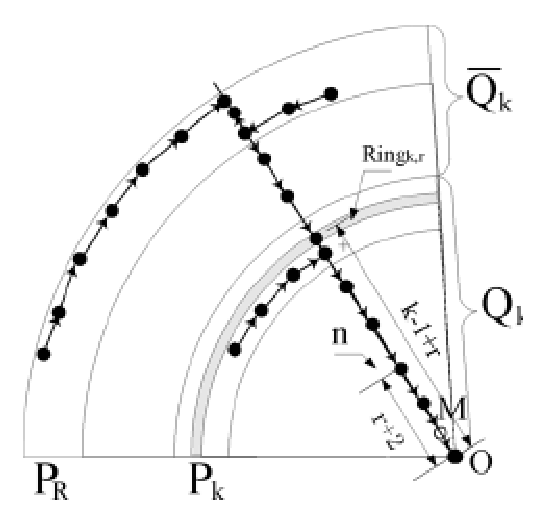
\includegraphics[scale=0.4]{images/extending_lifetime_1.eps}
\caption{}
\label{fig:extending_lifetime_path}
\end{subfigure}
\begin{subfigure}{0.5\textwidth}
\centering
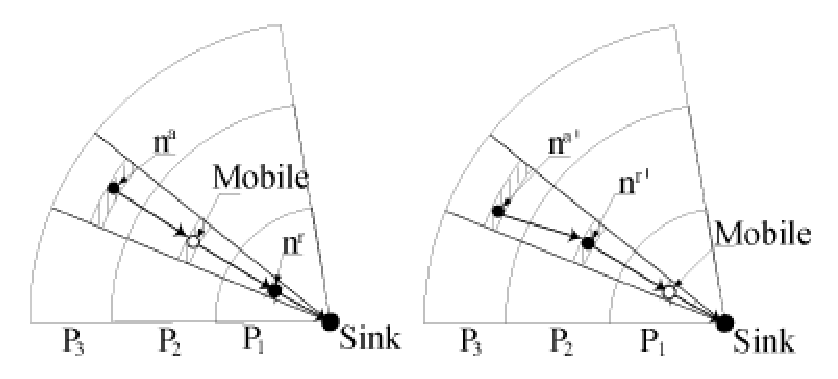
\includegraphics[scale=0.5]{images/extending_lifetime_2.eps}
\caption{}
\label{fig:extending_lifetime_depletion}
\end{subfigure}
\caption{Η διαδρομή που ακολουθούν τα πακέτα (α') και ο τρόπος που εκμεταλεύεται τους 2-hop γείτονες της στατικής Πηγής ο κινητός κόμβος (β'). }
\label{fig:}
\end{figure}
Όπως φαίνεται και στην εικόνα \ref{fig:extending_lifetime_depletion} ο κινητός κόμβος αντικαθιστά κάθε φορά έναν κόμβο από αυτούς που είναι 2-hop ή 1-hop μακριά και
χρησιμοποιεί τον άλλον (ο οποίος βρίσκεται πάνω στην ακτίνα που σχηματίζεται από τον κινητό κόμβο και την στατική Πηγή έστω $r$) μέχρι να του εξαντλήσει τελείως την
ενέργειά του. Κάθε φορά που ο κινητός κόμβος επιλέγει έναν νέο κόμβο $u_{i}\in G$ τότε όλοι οι κόμβοι οι οποίοι ανήκουν στην ακτίνα $r$ λαμβάνουν όλα τα πακέτα από
όλους του κόμβους που ανήκουν στο ίδιο δαχτυλίδι. Δηλαδή οι κόμβοι που ανήκουν σε έναν δακτύλιο στέλνουν τα πακέτα τους πάνω από αυτόν δακτύλιο μέχρι να φτάσουν στον
κόμβο που ανήκει στην ακτίνα $r$ όπως φαίνεται και στην εικόνα \ref{fig:extending_lifetime_path}. Οι συγγραφείς αποδυκνύουν αναλυτικά οτι με αυτό το σχήμα το δίκτυο
μπορεί να έχει χρόνο ζωής  $T>4\frac{E}{R^{2}e}-\frac{16E}{R^{4}e}$ δεδομένου οτι για την ακτίνα του δικτύου $R$ ισχύει $R>16\pi+4$. Χρησιμοποιώντας την ίδια λογική
αποδεικνύεται οτι για $m$ κινητούς κόμβους (οι οποίοι εκμεταλεύονται $2m$ στατικούς κόμβους πάνω στην ακτίνα $r$) ο χρόνος ζωής του δικτύου φράσεται από την σχέση:
\begin{align*}
T>4m\frac{E}{R^{2}e}-\frac{32\pi m^{3}E}{R^{4}e} \qquad\text{αν η ακτίνα $R$ είναι αρκετά μεγάλη}
\end{align*}
Τα πειράματα αυτής της εργασίας έδειξαν οτι ο χρόνος ζωής αυξάνεται σημαντικά και επαληθεύονται τα προηγούμενα θεωρητικά αποτελέσματα. Όπως έγινε εμφανές η εργασία
αυτή ακολουθεί μια διαφορετική λογική από τις υπόλοιπες σχετικές εργασίες το οποίο την κάνει ξεχωριστή.

Μια επίσης διαφορετική εργασία στο \cite{auction_energy_balance}. Στην εργασία αυτή θεωρείται ένα υβριδικό δίκτυο αισθητήρων το οποίο αποτελείται από κινητούς
κόμβους και στατικούς κόμβους. Στο μοντέλο θεωρείται οτι οι κινητοί κόμβοι έχουν πολύ περισσότερη ενέργεια από τους στατικούς, ο χρόνος χωρίζεται σε γύρους και η
εργασία επικεντρώνεται στην κατάλληλη διαχείρηση των κινητών κόμβων σε έναν γύρο. Να σημειωθεί οτι αποτελεί από τις λίγες εργασίες που παίρνει υπόψην στο μοντέλο της
και στοχεύει στην μείωση της κατανάλωσης την ενέργεια που σπαταλάται για την κίνηση ενός κινητού κόμβου. Οι συγγραφείς προτείνουν αρχικά έναν καθολικό (centralized)
αλγόριθμο και στην συνέχεια έναν κατανεμημένο αλγόριθμο. O κατανεμημένος αλγόριθμος χρησιμοποιεί μια διαφορετική προσέγγισει για να λύσει το πρόβλημα της
δρομολόγησης των κινητών κόμβων. Αρχικά η περιοχή του δικτύου χωρίζεται σε ένα πλέγμα (grid) και κάθε κελί εκλέγει έναν στατικό κόμβο ως αρχηγό. Ο χρόνος χωρίζεται
περεταίρω σε 3 διαφορετικές φάσεις ενός γύρου:
\begin{itemize}
\item \textbf{Φάση διάδοσης:} Αρχικά ο αρχηγός κάθε κελιού μέσα στο πλέγμα συλλέγει τις τοποθεσίες των γεγονότων από τους στατικούς αισθητήρες. Επίσης συλέγει τις
αναφορές (τοποθεσία, ενέργια) των κινητών κόμβων. Στην συνέχεια η ύπαρξη των κινητών κμόβων διαφημίζεται από τα κελιά που τους περιέχουν.
\item \textbf{Φάση διαγωνισμού:} Κάθε κελί του πλέγματος που περιέχει ένα γεγονός (και επομένως πρέπει να έρθει ένας κινητός κόμβος για να το συλλέξει) διαγωνίζεται
με όλα τα άλλα αντίστοιχα κελιά για τους κινητούς κόμβους χρησιμοποιώντας προσκλήσεις. Ο κάθε κινητός κόμβος αποδέχεται ή απορρήπτει μια πρόσκληση ανάλογα με τα
δεδομένα της πρόσκλησης όπως π.χ η απόσταση του γεγονότος από τη θέση του κινητού κόμβου.
\item \textbf{Φάση δρομολόγησης:} Ο κάθε κινητός κόμβος αφού έχει επιλέξει μια σειρά από κελιά τότε εκτελεί την διαδρομή του χρησιμοποιώντας προσεγγιστικό αλγόριθμο
του προβλήματος TSP.
\end{itemize}
Αποδεικνύεται οτι η πολυπλοκότητα του αλγορίθμου είναι $O(m\cdot\hat{M} + n\cdot\hat{N} + m^{2}h)$ όπου $m,n$ οι κινητοί και στατικοί κόμβοι αντίστοιχα, $\hat{M},
\hat{N}$ οι διαστάσεις του πλέγματος και $h$ η διάμετρος του δικτύου. Οι προσομοιώσεις δείξαν οτι υπάρχει σημαντική αύξηση του χρόνου ζωής του δικτύου.



\section{Εναλλακτικές Τεχνικές} % node density(normal distribution)
Εκτός από τους αλγόριθμους δρομολόγησης υπάρχουν και άλλες τεχνικές που έχουν μελετηθεί με σκοπό την επέκταση του χρόνου ζωής ενός ασύρματου δικτύου αισθητήρων.
Έχουν μελετηθεί τεχνικές που έχουν να κάνουν με αξοιοποίηση εναλλακτικών πηγών ενέργειας όπως είναι η ηλιακή ενέργεια, τεχνικές που θεωρούν πιο ισχυρά μοντέλα όπως
η πρόσθεση επιπλέον κόμβων σε ένα δίκτυο εκεί που χρειάζεται αλλά και τεχνικές... Τέλος παρουσιάζεται μια νές πρωτοπόρα ριζοσπαστική τεχνική, αυτή της ασύρματης
φόρτισης, η οποία αναλύεται εκτενέστερα στο κεφάλαιο \ref{ch:wrsns}.

\subsection{Τεχνικές εναλλακτικών πηγών ενέργειας}
Οι τεχνικές αυτές ασχολούνται με την αξιοποίηση εναλλακτικών πηγών ενέργειας (energy harvesting) προκειμένου να φορτίσουν τους στατικούς κόμβους που επιβλέπουν το
περιβάλλον. τα τελευταία χρόνια αυτές οι τεχνικές έχουν γνωρίσει μεγάλη ανάπτυξη και έχουν ενσωματωθεί επιτυχημένα σε συστήματα ΑΔΑ. Υπάρχει ποικιλία διαφορετικών
ενεργειών που μπορούν να χρησιμοποιηθούν για την αύξηση ζωής του δικτύου όπως μηχανική, θερμική και ηλιακή ενέργεια η οποία μπορεί να μετατραπεί σε ηλεκτρική και να
ενεργοποιήσει τους κόμβους ή απλώς να επαναφορτήσει τις μπαταρίες τους. Η πιο πολυχρησιμοποιούμενη είναι η ηλιακή ενέργεια. Για την ηλιακή ενέργεια ο ρυθμός
επαναφόρτισης ορίζεται από τον παρακάτω τύπο:
\begin{align*}
\pi_{r} = Rad_{s} \times \eta_{\rho} \times \rho_{e} \times A
\end{align*}
όπου to $Rad_{s}$ αντιστοιχεί στην ηλιακή ακτινοβολία, το $\eta_{\rho}$ αντιστοιχεί στην αποδοτικότητα του ηλιακού συλλέκτη να μετατρέψει την ηλιακή ενέργεια σε
ηλεκτρική ενέργεια, το $\rho_{e}$ αντιστοιχεί στην απόδοση του ηλεκτρικού κυκλώματος και το $A$ αντιστοιχεί στο μέγεθος του ηλιακού συλλέκτη.

Ωστόσο καθώς όλες αυτές οι εναλλακτικές ενέργειες προέρχονται από το εξωτερικό περιβάλλον οι χωροχρονικοί χαρακτήρες τους έχουν μεγάλες διακυμάνσεις όσον αφορά την
απόδοση τους η οποία συνήθως είναι χαμηλή και ευέσθητη στην δυναμική του περιβάλλοντος. Για παράδειγμα σε ένα σύστημα βασισμένο στην ηλιακή ενέργεια, η ισχύς εξόδου
του η οποία θα τροφοδοτήσει έναν αισθητήρα καθορίζεται από τις ηλιακές ακτίνες που προσάπτονται εκείνη την στιγμή στους ηλιακούς συλλέκτες και μεταβάλλεται σημαντικά
ανάλογα με την ώρα και τον καιρό. Στατιστικές έχουν δείξει οτι υπάρχει διαφορά μέχρι και 3 τάξεις μεγέθους στην διαθέσιμη ενέργεια ανάμεσα σε μια σκιώδης,
συννεφιασμένης και ηλιόλουστης μέρας \cite{harvesting_comparison}. Καθώς δεν υπάρχει γενικά τρόπος να γνωρίζει εξ'αρχής κανείς την κατάσταση που θα υπάρχει στο δίκτυο
αισθητήρων υπάρχει μεγάλη δυσκολία στο σχεδιασμό πρωτοκόλλων που εκμεταλεύονται τέτοιες μορφές ενέργειας και να κρατάνε τους κόμβους πάντα ενεργούς. Αυτό όμως είναι
πολύ δύσκολο ειδικά σε εφαρμογές στις οποίες το κύριο έργο είναι να συλλέγουν περιοδικά δεδομένα και πληροφορίες από όλους τους κόμβους. Στην περίπτωση που κάποιοι
αισθητήρες καταναλώσουν όλη την ενέργειά τους και δεν επαναφορτιστούν γρήγορα, το δίκτυο σταδιακά θα καταρεύσει. Υπάρχουν όμως πρωτόκολλα που ρυθμίζουν τις
λειτουργίες του κάθε κόμβου ανάλογα με την κατάσταση που επικρατεί στο εξωτερικό του περιβάλλον και παρουσιάζονται στην συνέχεια.

Μία από τις πρώτες εργασίες παρουσιάζεται στο \cite{heliomote}. Στην εργασία αυτή παρουσιάζεται ένα σύστημα του οποίου οι κόμβοι έχουν ηλιακούς συλλέκτες
και μπορούν να φορτίζονται από την ηλιακή ενέργεια όπως φαίνεται στην εικόνα \ref{fig:heliomote_example}.
\begin{figure}[h]
	\centering
	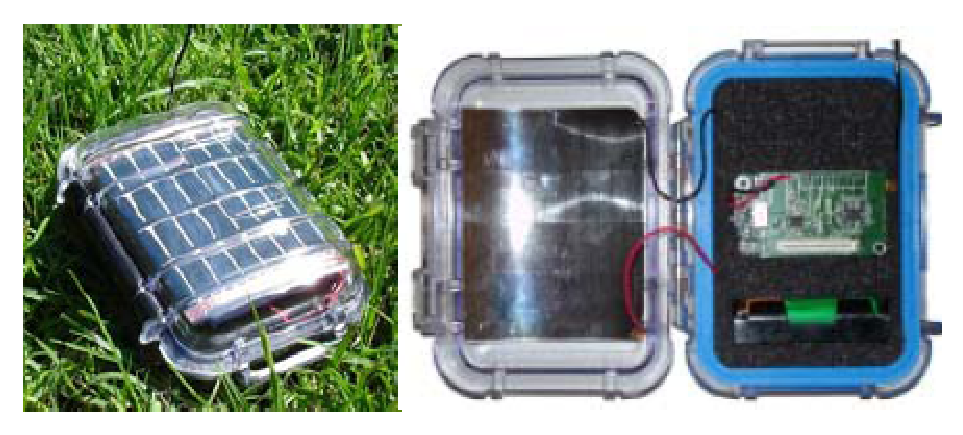
\includegraphics[width=0.8\textwidth]{images/heliomote_example.eps}
	\caption{Ένας κόμβος του συστήματος \textit{Heliomote}.}
	\label{fig:heliomote_example}
\end{figure}

Με αυτόν τον τρόπο το σύστημα μπορεί να επιμηκύνει το χρόνο ζωής του συλλέγοντας ενέργεια από τον ήλιο. Επιπλεόν στην εργασία προτείνεται ένας εναλλακτικός τρόπος
δρομολόγησης των πακέτων. Συγκεκριμένα, τα πακέτα δρομολογούνται μέσα από μονοπάτια τα οποία έχουν το μεγαλύτερη συλλογή ηλιακής ενέργειας. Επίσης κόμβοι οι οποίοι
έχουν μικρή συλλογή ηλιακής ενέργειας (π.χ. είναι κάτω από ένα δέντρο) τότε μειώνουν τον φόρτο εργασίας τους εσκεμένα. Υπάρχει επομένως εξισορρόπηση της ενέργειας
του δικτύου.

Στην εργασία \cite{harvesting_6} μελετάται η περίπτωση ενός ασύρματου δικτύου αισθητήρων στο οποίο υπάρχει πλεονασμός κόμβων οι οποίοι μπορούν να
επαναφορτιστούν. Η εργασία αναλύει το πρόβλημα του πως οι κόμβοι θα έπρεπε να ενεργοποιούνται δυναμικά έτσι ώστε να μεγιστοποιηθεί η κάλυψη του δικτύου. Αφού δειχθεί
η βέλτιστη λύση, στην συνέχεια προτείνεται μια κατανεμημένη πολιτική ενεργοποίησης η οποία επιτυγχάνει το $\frac{3}{4}$ της βέλτιστης λύσης ενώ παρέχονται
προσομοιώσεις που επιβεβαιώνουν τα θεωρητικά αποτελέσματα.

Στην εργασία \cite{harvesting_7} αναλύεται η απόδοση πολυ-βηματικών (multi-hop) μεταδόσεων στην περίπτωση που υπάρχει δυνατότητα επαναφόρτισης ορισμένων κόμβων. Στην
συνέχεια σχεδιάζεται ένας αλγόριθμος ο οποίος λαμβάνει υπόψην του την αναπλήρωση ενέργειας των κόμβων και προωθεί τα πακέτα προς αυτούς τους κόμβους ο οποίος είναι
ασυμπτωτικά βέλτιστος σε αντιστοιχία με το μέγεθος του δικτύου. Ο αλγόριθμος δεν θεωρεί κάποια στατιστική πληροφορία όσον αφορά την άφιξη των πακέτων και επομένως
μπορεί να ενσωματωθεί σε ήδη υπάρχοντα σχήματα δρομολόγησης (προληπτικά ή κατ'απαίτηση). Τα αποτελέσματα των προσομειώσεων επιβεβαιώσαν οτι ο αλγόριθμος πετυχαίνει
να μεγιστοποιήσει την απόδοση σε ενεργειακά (energy-aware) δίκτυα.

Στις εργασίες \cite{harvesting_8} \cite{harvesting_9} αναλύεται ξανά η βέλτιστη δειγματοληψία των κόμβων κάτω από τους περιορισμούς των εναλλακτικών ενεργειών όπως
είναι η φωτεινότητα στην ηλιακή ενέργεια. Σε κάθε περίπτωση προτείνεται ένας κατανεμημένος αλγόριθμος ο οποίος ρυθμίζει κατάλληλα τον ρυθμό δειγματοληψίας του κάθε
κόμβου και λύνει το πρόβλημα αποδοτικά. Τέλος εκτελούνται προσομοιώσεις που αποδεικνύουν την απόδοση του εκάστοτε αλγορίθμου.



\subsection{Τεχνικές αυξησης των κόμβων του δικτύου}
Στην τεχνική αυτή υπάγονται εργασίες οι οποίες αναλύουν την βέλτιστη κατανομή των κόμβων σε ένα ασύρματο δίκτυο αισθητήρων και εργασίες που προτείνουν αποδοτικούς
τρόπους για την αντικατάσταση κόμβων του δικτύου οι οποίοι έχουν χάσει πλήρως την ενέργειά τους. Στην πρώτη περίπτωση εκτελείται ένας προληπτικός αλγόριθμος (offline
algorithm) ο οποίος βρίσκει την βέλτιστη την βέλτιστη ανάπτυξη των αισθητήρων κάτω από συγκεκριμένες συνθήκες. Στη δεύτερη περίπτωση εκτελούνται αλγόριθμοι άμεσης
απόκρισης (online algorithms) οι οποίοι αφού αναλύσουν την κατάσταση του δικτύου, βρίσκουν το βέλτιστο υποσύνολο του δικτύου το οποίο θα πρέπει να αντικατασταθεί ή
να προστεθούν επιπλέον κόμβοι.

Στην εργασία \cite{gaussian_sensors} οι συγγραφείς αναλύουν την περίπτωση όπου οι κόμβοι δεν τοποθετούνται ομοιόμορφα κατανεμημένα αλλά με βάση την Gaussian κατανομή
σε δισδιάστατιο χώρο. Στην συνέχεια εντοπίζουν κάτω από συγκεκριμένες υποθέσεις και ιδιότητες της Gaussian κατανομής μπορεί να επιτευχθεί η επιθυμητή καλυψη και
διάρκεια ζωής του δικτύου. Αφού αναλύσουν τις στρατηγικές ανάπτυξης των κόμβων προτείνουν 2 αλγόριθμους ανάπτυξης των κόμβων οι οποίοι αυξάνουν σημαντικά τον χρόνο
ζωής του δικτύου.

Η εργασία στο \cite{sens_deployment3} εισάγει για πρώτη φορά στο μοντέλο των ΑΔΑ την έννοια της πρόσθεσης ή αντικατάστασης κόμβων του δικτύου ενώ ενσωματώνει στο
μοντέλο την έννοια της ετερογένειας, της ύπαρξης δηλαδή διαφορετικών κόμβων ως προς τις δυνατότητές τους. Με τις προαναφερθείσες παραδοχές αυξάνεται σημαντικά η
δυναμικότητα του δικτύου που μελετάται και οι συγγραφείς διαπιστώνουν οτι ο μόνος τρόπος για την αποδοτική διαχείρηση της ενέργειας είναι μέσα από αλγόριθμους
μάθησης. Συγκεκριμένα, οι συγγραφείς αναπτύσουν έναν κατανεμημένο αλγόριθμο ελαχιστοποίησης της ενέργειας ο οποίος χρησιμοποιεί τοπικές πληροφορίες όπως για
παράδειγμα πυκνότητα και ενέργεια του δικτύου σε μια τοπική περιοχή και ρυθμίζει κατάλληλα την πολιτική ύπνου (sleeping policy) των κόμβων. Οι προσομειώσεις δείξαν
οτι με αυτόν τον τρόπο διπλασιάζετα σχεδόν ο λόγος επιτυχίας σε σύγκριση με το Directed Diffusion ενώ μαζί με την προσθήκη ετερογενών κόμβων σε κατάλληλα σημεία του
δικτύου ο λόγος επιτυχίας αυξάνεται ακόμα περισσότερο με παρόμοια ενεργειακή συμπεριφορά.

Η εργασίες στα \cite{sens_deployment1} \cite{sens_deployment2} μελετάνε την περίπτωση ενός δικτύου το οποίο λειτουργεί για πολύ μεγάλο χρονικό διάστημα. Για να
λύσουν το πρόβλημα που δημιουργείται από τους περιορισμένους πόρους ενέργειας που έχει ο κάθε κόμβος προτείνουν μια στρατηγική αντικατάστασης και ανάκτησης των παλιών
κόμβων με καινούργιους. Για την υλοποίηση της ιδέας χρησιμοποιείται ένα μηχανικά κινούμενο ρομπότ το οποίο έχει την ικανότητα να αντικαθιστά τους κόμβους του
δικτύου. Το ρομπότ αυτό περιοδικά διασχίζει την περιοχή του δικτύου και εγκαθιστά καινούργιους κόμβους ενώ επιστρέφει τους παλιούς κόμβους στην βάση για επαναφόρτηση.


\subsection{Τεχνικές επαναφόρτισης κόμβων} \label{sc:recharg_tecnhiques}
Η πρόσφατη πρόοδος στις περιοχές των υλικών που χρησιμοποιούνται για τις μπαταρές αλλά και στην περιοχή της ασύρματης μετάδοσης ενέργειας προσφέρουν νέες δυνατότητες
διαχείρησης της διαθέσιμης ενέργειας. Στην πρώτη περιοχή ανακαλύφθηκε ένα νέο υλικό για μπαταρίες το οποίο επιτρέπει πολύ γρήγορες φορτίσεις και αργές ξεφορτίσεις
\cite{fast_recharging}. Η ανακάλυψη αυτή συνδυάζει τα πλεονεκτήματα των κλασσικών $Li-ion$ μπαταριών και των υπερ-πυκνωτών χρησιμοποιώντας την τεχνολογία
$LiFePO_{4}$ επιτρέποντας φορτίσεις μέχρι και 400C\footnote{C ορίζεται ως η ονομαστική χωρητικότητα της μπαταρίας. Για παράδειγμα για μία
μπαταρία χωρητικότητας 1000mAh C=1000mA.}. Στη δεύτερη περιοχή η τεχνολογία γύρω από την ασύρματη μετάδοση ενέργειας έχει εξελιχθεί τόσο πολύ που πλέον τα ποσοστά
επιτυχίας έχουν ανέβει σημαντικά. Οι εργασίες στα \cite{wireless_recharg1}, \cite{wireless_recharg2}, \cite{wireless_recharg3} δείχνουν οτι μπορεί να υπάρξει μέχρι
και 60\% απόδοση στην μεταφορά ενέργειας. Ταυτόχρονα η Intel\textsuperscript{\textregistered} δείχνει μέχρι και 75\% απόδοση \cite{intel_recharg} ενώ η εταιρεία
Witricity\textsuperscript{\textregistered} ισχυρίζεται οτι μπορεί να επιτύχει μεταφορά ενέργειας με ποσοστό επιτυχίας μέχρι και 90\% \cite{witricity_90}. Η
συγκεκριμένη τεχνολογία έχει οδηγήσει σε έναν καινούργιο κλάδο των ασύρματων δικτύων ασιθητήρων: τα ασύρματα επαναφορτιζόμενα δίκτυα αισθηρήτων (ΑΕΔΑ). Θα αναλυθεί
εκτενέστερα στο επόμενο κεφάλαιο αφού αποτελεί τον κινητήριο μοχλό για αυτή την διπλωματική εργασία.

























%3rd chapter


\chapter{Ασύρματα Επαναφορτιζόμενα Δίκτυα Αισθητήρων}\label{ch:wrsns}
Σε αυτό το κεφάλαιο θα αναλυθεί η τεχνολογία της ασύρματης μεταφοράς ενέργειας καθώς και η ιστορία της.
\section{Η Ιστορία Πίσω Από την Τεχνολογία}
Οι προσπάθειες ασύρματης μεταφοράς ενέργειας πρωτοσυναντόνται πίσω στα τέλη του 19ου αιώνα, πολύ πριν την εγκατάσταση ενσύρματης μεταφοράς ενέργειας. Ο Νικόλα Τέσλα
από το 1891 είχε καταφέρει να μεταφέρει ενέργεια ασύρματα μέσα από επαγωγή μεγάλων πηνείων. Η εφεύρεση αυτή τον είχε εντυπωσιάσει τόσο πολύ όσο τίποτα άλλο που
μάλιστα δήλωσε οτι αυτή η εφεύρεσή του θα ήταν η πιο πολύτιμη από όλες. Tο 1899, ο Νικολά Τέσλα, μεταφέρθηκε στα εργαστήρια της εταιρείας Colorado Springs όπου
εμβάθυνε ακόμα περισσότερο στην τεχνολογία αυτή. Το 1902 κατέθεσε μια πατέντα \cite{tesla_patent} για μία συσκευή η οποία ήταν προιόν αυτής της έρευνας. Ήταν ένα
πηνίο σε διάταξη Τέσλα το οποίο μετέφερε ενέργεια χρησιμοποιώντας μεταφορά ενέργειας σε ιδιοσυχνότητα από το κάτω πηνίο σε μερικά μέτρα στο πάνω πηνίο. Αυτό
επιτρέπει να δημιουργηθούν πολύ υψηλές τάσεις και χρησιμοποιείται αρκετά στην πράξη σήμερα.

\begin{figure}[h]
  \centering
  \subfloat{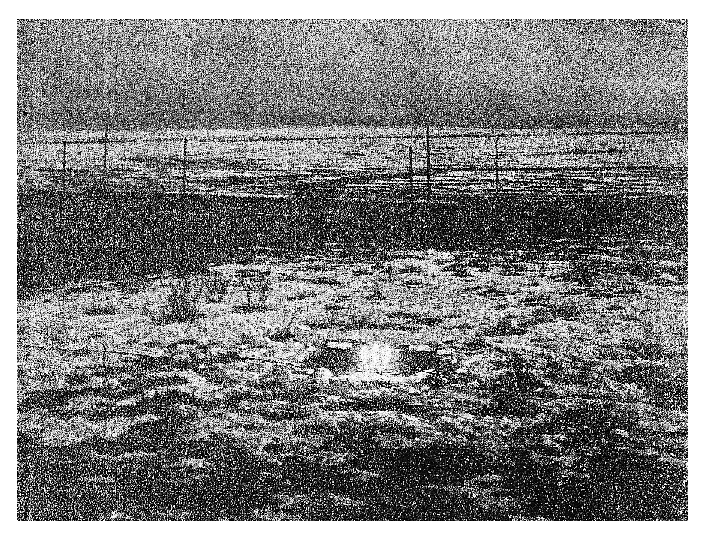
\includegraphics[width=0.62\textwidth]{images/tesla_exper1.eps}}
  \subfloat{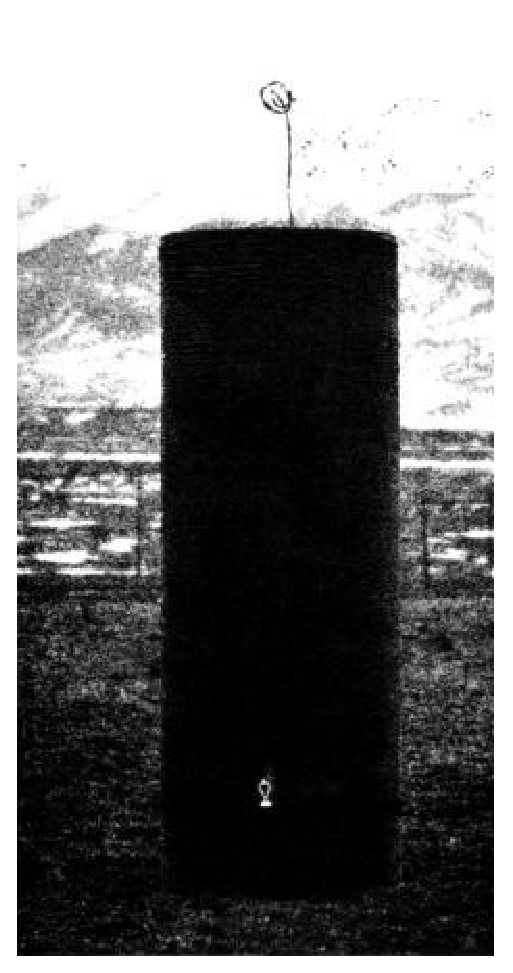
\includegraphics[width=0.32\textwidth]{images/tesla_exper2.eps}}
  \caption{Επιτυχημένες προσπάθειες του Νικόλα Τέσλα μεταφοράς ασύρματης ενέργειας είχαν γίνει από τα τέλη του 19ου αιώνα.}
  \label{fig:tesla_eperiments}
\end{figure}

Εκείνη την εποχή ήταν η ανατολή για την θέσπιση ηλεκτρικής ενέργειας στις συσκευές. Επίσης εκείνη την εποχή μόλις είχε τελειώσει ο πόλεμος των ρευμάτων (the war of
currents) στον οποίο υπήρχαν διαφωνίες στο αν θα έπρεπε στα ηλεκτρικά δίκτυα που επρόκειτο να δημιουργηθούν να είχαν εναλλασσόμενο ρεύμα (AC) ή συνεχές (DC). Όμως
υπήρχαν επιστήμονες και μηχανικοί που συμφωνούσαν οτι η χρησιμοποιήση καλωδίων για την μεταφορά ενέργειας από κάθε τοποθεσία που αναπαράγοταν σε κάθε τοποθεσία που
θα το χρησιμοποιούσε θα ήταν πολύ ακριβό και όχι πρακτικό. Ο Τέσλα ήταν ένας από τους πιο γνωστούς επιστήμονες της εποχής υποστήριζε αυτή την άποψη και προσπαθούσε
να βρει τρόπους να μεταφέρει ενέργεια ασύρματα. Το όραμά του ήταν ένας ασύρματος κόσμος στον οποίο η ασύρματη μεταφορά ενέργειας και η ασύρματες επικοινωνίες θα
μπορούσαν να φτάσουν σε όλο τον κόσμο, παραδίδοντας ενέργεια και πληροφορίες σε πλοία τα οποία ταξιδεύουν στη θάλασσα, σε εργοστάσιο και γενικά σε κάθε σπίτι του
πλανήτη.

Ο Τέσλα έχοντας πάρει μια χορήγησει US\$150.000, ξεκίνησε να κατασκευάζει τον πύργο Wardenclyffe προκειμένου να κάνει το όραμά του πραγματικότητα. Η κατασκευή είχε
ύψος 56 μέτρα και είχε χτιστεί κοντά στην Νέα Υόρκη ενώ το κτήριο κάτω από τον πύργο χρησιμοποιόταν για ως εργαστήριο. Για την λειτουργία του όμως ο Tέσλα χρειαζόταν
επιπλέον χρηματοδοτήσεις τις οποίες ζητούσε αλλεπάλληλα από τον John Pierpont Morgan ο οποίος ήταν κύριος χορηγός του. Ωστόσο ο J. P. Morgan δεν πείστηκε από τις
ικανότητες του κατασκευάσματος του Τέσλα και έτσι σταμάτησε την χρηματοδότηση με συνέπεια το σχέδιο του Τέσλα να σταματήσει εκεί.

\begin{figure}[h]
	\centering
	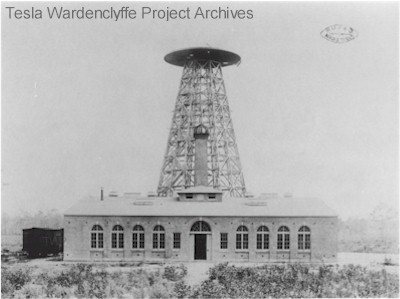
\includegraphics[width=\textwidth]{images/Wardenclyffe_Tower.jpg}
	\caption{Ο πύργος Wardenclyffe ο οποίος χτίστηκε για πειράματα μεταδοσης ασύρματης ενέργεια.}
	\label{fig:Wardenclyffe_Tower}
\end{figure}

Παρόλο που για την εποχή του, ο Τέσλα είχε κατασκευάσει ένα πολύ προηγμένο σύστημα μεταφοράς ενέργειας, είχε πολλά προβλήματα με κύριο τις απώλειες ενέργειας. Καθώς
η συσκευή του Τέσλα εξεπεμπε στον χώρο πολύ δυνατά ηλεκτρομαγνητικά κύματα, προκειμένου να πετύχει μεταφορά ενέργειας σε μεγάλη απόσταση χρειαζόταν τεράστιες
ποσότητες ενέργειας καθώς οι απώλειες ήταν πολύ μεγάλες.

Στις αρχές της δεκαετίας του 1960 η μεταφορά ενέργειας μέσω ιδιοσυχνοτικής ηλεκτρομαγνητικής επαγωγής (resonant inductive coupling) χρησιμοποιήθηκε επιτυχημένα σε
εμφυτεύσιμες συσκευές της ιατρικής όπως βηματοδότες και τεχνητές καρδιές. Τα πρώτα συστήματα είχαν μόνο δέκτη ιδιοσυχνοτικού πηνίου αλλά τα επόμενα συστήματα
ενσωμάτωσαη και πομό ιδιοσυχνοτικού πομπού. Οι συσκευές αυτές είχαν σχεδιαστεί έτσι ώστε να έχουν πολύ μεγάλη απόδοση χρησιμοποιώντας χαμηλής κατανάλωσης
ηλεκτρονικά. Ακόμα και σήμερα αυτή η μέθοδος χρησιμοποιείται σε εμπορικά διαθέσιμα ιατρικά εμφυτεύματα.

Από τότε η πρόοδος στην ασύρματη μεταφοράς ενέργειας υπήρξε ελάχιστη για πολλές δεκαετίες. Στις αρχές του 1990 η ανάγκη για ασύρματη μεταφορά ενέργειας
ξαναναδύθηκε καθώς οι φορητές συσκευές έγιναν πολύ δημοφιλής. Ένας πειραματικός λεωφορείοδρομος κατασκευάστηκε το 1994 \cite{bus_coil} το οποίο επέτρεπε
αποδοτικότητα 80\% καθώς επαναφόρτιζε την μπαταρία ενός πρωτότυπου λεωφορείου μέσω ιδιοσυχνοτικής ηλεκτρομαγνητικής επαγωγής καθώς αυτό κινείτο. Επιπλέον μελετήθηκε η
φόρτιση του λεωφορείο όταν αυτό είναι σταματημένο σε στάσεις και σε γκαράζ. Η απόσταση μεταξή του πηνίου πομπού και του πηνίου δέκτη είχε σχεδιαστεί έτσι ώστε να
είναι μικρότερη από 10 εκατοστά.

Πρόσφατα, ασύρματη μετάδοση ενέργειας επιτεύχθηκε βασισμένη σε ραδιοσυχνότητες μεταξύ των 850MHz και 950MHz (με κεντρική ραδιοσυχνότηα τα 915MHz) ερευνήθηκε. Κάτω
από αυτό το μοντέλο, ένας RF πομπός μεταδίδει ραδιοκύματα στην συχνότητα των 915MHz  και ένας RF δέκτης συχρονίζει στην ίδια ακριβός συχνότητα προκειμένου να
συλλέξει την ενέργεια. Ωστόσο αποδείχθηκε οτι τέτοια συστήματα μπορούν έχουν πολύ μικρή απόδοση καθώς έχουν μεγάλες απώλειες ακτινοβολίας. Η τεχνολογία επίσης είναι
ευαίσθητη σε εμπόδια μεταξύ του δέκτη και του πομπού ενώ θέτει ζητήματα υγείας γι'αυτό η χρήση της είναι περιορισμένη.

Μία δημοσίευση από το πανεπιστήμιο του MIT στα τέλη του 2007 ήρθε να ταράξει τα νερά στην τεχνολογία της ασύρματης μεταφοράς ενέργειας. Οι εργασία που αποτελείται
από τους Aristeidis Joannopoulos and Solja\v{c}i\'{c} και έχει τραβήξει το ενδιαφέρον της επιστημονικής κοινότητας. Στην εργασία παρουσιάζεται ένα πρότυπο σύστημα το
οποίο χρησιμοποιεί δύο ισχυρά συνδεδεμένα πηνία με την ίδια ιδιοσυχνότητα, ένας πομπός και ένας δέκτης, σε απόσταση 2 μέτρων. Στον πομπό δημιουργείται εναλλασσόμενο
ρεύμα το οποίο μέσω επαγωγής ο δέκτης λαμβάνει τα ηλεκτρομαγνητικά κύματα με απόδοση 40\% τα οποία μέσω του πηνίου μετατρέπονται σε ηλεκτρισμό και ανάβει μια λάμπα
40Watt. Το πείραμα φαίνεται στην εικόνα

Αμέσως μετά η Intel\textsuperscript{\textregistered} δείχνει μέχρι και 75\% απόδοση \cite{intel_recharg} ενώ η εταιρεία Witricity\textsuperscript{\textregistered}
ισχυρίζεται οτι μπορεί να επιτύχει μεταφορά ενέργειας με ποσοστό επιτυχίας μέχρι και 90\% \cite{witricity_90} για απόσταση μέχρι 20 εκατοστά.


\section{Επεξήγηση της Τεχνολογίας}
Η τεχνολογία πάνω στην οποία βασίζεται η ασύρματη μεταφορά ενέργειας μέσω ισχηρών συνδεδεμένων ιδιοσυχνοτήτων (strongly coupled resonance) βαστάει πάνω στις βασικές
αρχές του ηλεκτρομαγνητισμού, από την εποχή που ο Νικόλα Τέσλα είχε καταφέρει ασύρματη μεταφορά ενέργειας. Η διαφορά με την σημερινή μορφή της είναι οτι
η μεταφορά που είχε πετύχει ο Τέσλα είχε απώλειες ακτινοβολίας, ενώ ταυτόχρονα τα πηνία Τεσλα προορίζονταν για πολύ μεγάλες τάσεις και επομένως είχε άμεσες συνέπειες
στην υγεία του ανθρώπου.

Αν σε ένα δακτύλιο ο οποίος είναι κατασκευασμένος από αγώγιμο υλικό, εφαρμοστεί εναλλασσόμενο ρεύμα (AC) τότε αυτό θα παράξει ταλαντώμενο μαγνητικό πεδίο (oscillating
magnetic field) κάθετο στον άξονα του δακτύλιου όπως φαίνεται στην εικόνα \ref{fig:magnetic_field}. Λόγω της αυτεπαγωγής, η ταλάντωση θα σταματάει με ρυθμό ο
οποίος καθορίζεται άμεσα από τον παράγοντα Q (Q-factor)\footnote{Ο παράγοντας Q είναι ένας αριθμός ο οποίος περιγράφει τον ρυθμό με τον οποίο μια ταλάντωση (ή ένα
αντιηχείο (resonator) αντίστοιχα) αποσβαίνει. Όσο πιο υψηλός είναι ο αριθμός σημαίνει οτι ο ρυθμός απώλειας της ενέργειας λόγω αποσβέσεων είναι μικρότερος. Στην
πράξη μπορούν να φτιαχτούν ταλατωντές που έχουν $Q=10^{4}$ και μεγαλύτερο. Για ένα RLC κύκλωμα δίνεται από τον τύπο $Q=\frac{1}{r}\sqrt{\frac{C}{L}}$.}.
\begin{wrapfigure}{r}{0.5\textwidth}
  \vspace{-20pt}
  \begin{center}
  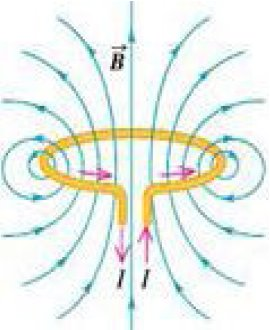
\includegraphics[width=0.48\textwidth]{images/inductive_ring.jpg}\label{fig:magnetic_field}
  \end{center}
  \vspace{-20pt}
  \caption{Το μαγνητικό πεδίο που δημιουργείται πάνω σε έναν αγώγιμο δακτύλιο καθώς σε αυτόν περνά εναλλασσόμενο ρεύμα.}
  \vspace{-10pt}
\end{wrapfigure}
Στην συνέχεια, αν ένας δεύτερος δακτύλιος έρθει κοντά στον πρώτο δακτύλιο τότε μπορεί να "πιάσει" κάποιο μέρος του μαγνητικού πεδίου το οποίο στην συνέχεια
δημιουργεί, επειδή είναι ταλαντούμενο το μαγνητικό πεδίο, ένα εναλλασσόμενο ρεύμα πάνω του. Το ρεύμα που δημιουργείται στο δεύτερο δακτύλιο μπορεί να χρησιμοποιηθεί
για να τροφοδοτήσει ηλεκτρικές συσκευές.  Αυτό το σύστημα μετάδοσης ενέργειας (ή καλύτερα μετατροπής της ενέργειας) χρησιμοποιείται εδώ και πάνω από έναν αιώνα στους
ηλεκτρικούς μετατροπείς και ηλεκτρικές γεννήτριες.

Για την ασύρματη μεταφορά ενέργειας χρησιμοποιείται η ίδια λογική μόνο που αντί για απλούς δακτύλιους, χρησιμοποιούνται πολύ υψηλής ποιότητας πηνία τα οποία
παρουσιάζουν επίσης πολύ υψηλό παράγοντα Q που τους επιτρέπει να μεγαλώσουν την απόσταση μεταξύ τους σε σχέση με την προηγούμενη περίπτωση. Για να μεγαλώσει η απόδοση
του συτήματος τα δύο πηνία θα πρέπει να είναι επίσης ισχυρά συνδεδεμένα (strongly coupled), δηλαδή ο συντελεστής αμοιβαίας επαγωγής να είναι κοντά στο 1\footnote{Ο
συντελεστής αμοιβαίας επαγωγής είναι πάντα μεταξύ του 0 και του 1 και εξαρτάται από την διάταξη των 2 πηνίων. Ουσιαστικά πρόκειται για το ποσοστό της μαγνητικής ροής
του πρώτου πηνίου/δακτύλιου κλπ "κόβει" το δεύτερο πηνίο/δακτύλιο κλπ. Μικρός συντελεστής σημαίνει οτι τα πηνία είναι ασθενά συνδεδεμένα και επομένως στο 2ο πηνίο
χάνεται το μεγαλύτερο μέρος της μαγνητικής ροής. Αντίθετα ισχυρά συνδεδεμένα σημαίνει οτι "κόβεται" μεγάλο μέρος της μαγνητικής ροής.}.

Η διαφορά με τις μέχρι τώρα προσπάθειες είναι οτι σε αυτό το μοντέλο προκειμένου να επιτευχθεί μεγαλύτερη απόδοση στην μεταφορά ενέργειας, θα πρέπει ο πομπός και ο
δέκτης έχουν και οι 2 την ίδια φυσική συχνότητα, δηλαδή τα 2 αυτά πηνεία θα πρέπει
να έχουν την ίδια ιδιοσυχνότητα (resonance)\footnote{Η ιδιότητα της ιδιοσυχνότητας υπάρχει σε πολλά διαφορετικά συστήματα. Μπορεί να θεωρηθεί  ως  η φυσική
συχνότητα στην οποία η ενέργεια μπορεί να προστεθεί με βέλτιστη απόδοση στο σύστημα. Ένα παράδειγμα είναι αυτό της κούνιας που κάνει ένα παιδί, τοοποίο μπορεί να
θεωρηθεί ως μια ταλάντωση. Το παιδί μπορεί να κινείται μπρος-πίσω σε ρυθμό που καθορίζεται από το μήκος της κούνιας. Μπορεί να κάνει την κούνια να κινηνεί με
μεαλύτερο μήκος αν συχρονίσει ταυτόχρονα τις κινήσεις των χεριών και των ποδιών του με την κίνηση της κούνιας. Ένα άλλο χαρακτηριστικό παράδειγμα της ιδιοσυχνότητα
είναι η θραύση ενός ποτηριού γεμάτο με κρασί από μία πολύ συγκεκριμένη νότα (συχνότητα) που τραγουδάει ένας τραγουδιστής.}. Ταυτόχρονα η απόστασή τους να μην
υπερβαίνει το $\frac{1}{4}$ του μήκους κύματος του πομπού, προκειμένου ο δέκτης να λαμβάνει αρκετό μαγνητικό πεδίο. Ένα παράδειγμα του συνολικού συστήματος φαίνεται
στην εικόνα \ref{fig:mit_exper0}.    


\begin{figure}[h]
	\centering
	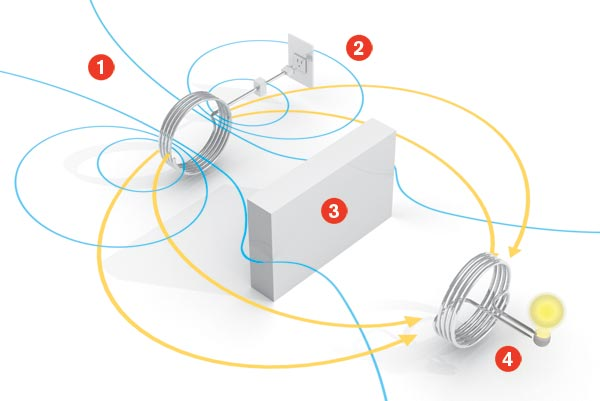
\includegraphics[width=0.9\textwidth]{images/mit_exper0.jpg}
	\caption{Ένα παράδειγμα της νέας τεχνολογίας ασύρματης μετάδοσης ενέργειας: (1) Πηνίο κατασκευασμένο από χαλκό με ιδιοσυχνοτητα.
    (2) Τροφοδοσία. (3) Εμπόδιο το οποίο προσπαρνάται χωρίς να υπάρχει απώλεια στην απόδοση. (4) Χάλκινο πηνίο με ίδια ιδιοσυχνότηα συνδεδεμένο με μια λάμπα.}
	\label{fig:mit_exper0}
\end{figure}


Οι ερευνητές του MIT επιτυχημένα παρουσίασαν στην πράξη αυτή την θεωρία. Χρησιμοποιώντας 2 χάλκινα πηνία με 5 γύρους, και διάμετρο 60 εκατοστά, τα οποία ήταν
τοποθετημένα σε απόσταση 2 μέτρων μεταξύ του, κατάφεραν να πετύχουν μεταφορά ενέργειας από το ένα πηνίο στο άλλο με απόδοση 45\% και τελικά τροφοδοτόντας μία λάμπα
60 Watt στο δεύτερο πηνίο. Τα πηνία ήταν σχεδιασμένα έτσι ώστε να έχουν ακριβώς την ίδια ιδιοσυχνότητα, στα 9,9MHz με μήκος κύματος τα 30 μέτρα και ήταν τοποθετημένα
ακριβώς στον ίδιο (κάθετο άξονα. Φωτογραφίες από το πείραμα φαίνονται στην εικόνα \ref{fig:mit_eperiments}.
\begin{figure}[h]
  \centering
  \subfloat{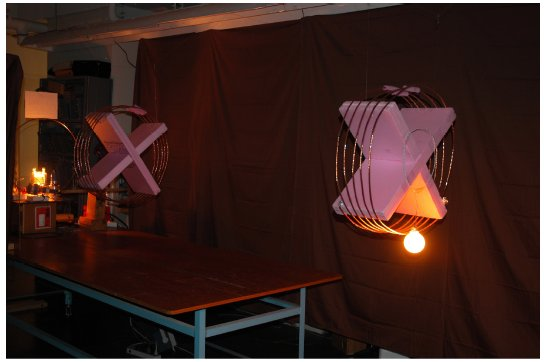
\includegraphics[width=0.48\textwidth]{images/mit_exper1.jpg}}
  \subfloat{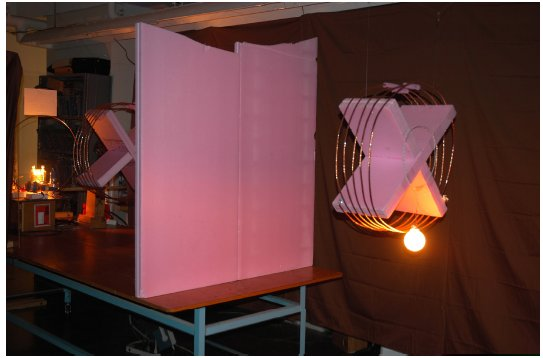
\includegraphics[width=0.48\textwidth]{images/mit_exper2.jpg}}
  \caption{Το πείραμα που έγινε στο mit είχε απόδοση κοντά στο 45\%.}
  \label{fig:mit_eperiments}
\end{figure}

Όπως φαίνεται και στις εικόνες, ακόμα και αν τοποθετούνταν ένα εμπόδιο ανάμεσα στα 2 πηνία, η λάμπα συνέχιζε να άναβε, δηλαδή η μεταφορά ενέργειας συνέχιζε να
υφίστατε με σχεδόν την ίδια απόδοση. Αυτό συνβαίνει λόγω της γεωμετρίας του μαγνητικού πεδίου που δημιουργείται.

Η τεχνολογία της ασύρματης μεταφοράς ενέργειας μπορεί άνετα να ενσωματωθεί στα ασύρματα δίκτυα αισθητήρων καθώς η λογική της είναι πολύ απλή. Ο κάθε κόμβος θα πρέπει
να έχει επιπλέον κυκλώματα με κύριο συστατικό το πηνίο το οποίο θα του επιτρέπει την φόρτισή του. Επίσης θα μπορεί να υπάρχει ένας κινητός κόμβος (robot) ο οποίος με
κατάλληλους αλγορίθμους θα κινείται στην περιοχή του δικτύου και θα φορτίζει τον κάθε κόμβο. Θα πρέπει όμως όλοι οι κόμβοι να έχουν συγκεκριμένη ιδιοσυχνότητα η
οποία θα είναι ίδια με την ιδιοσυχνότητα του πομπού, δηλαδή του κινητού κόμβου. Επίσης δεν θα είναι αναγκαίο ο κινητός κόμβος να έχει άμεση επαφή (<1 εκατοστού) με
τον στατικό κόμβο ανάλογα με το μήκος κύματος που θα χρησιμοποιείται ο κινητός κόμβος θα μπορεί να τον φορτίζει αποδοτικά και από πιο μακρινές αποστάσεις. Τέλος λόγω
των ιδιοτήτων της τεχνολογίας αυτής, ακόμα και αν υπάρχει ένα μικρό εμπόδιο το οποίο εμποδίζει την οπτική επαφή ανάμεσα στον κινητό κόμβο και τον στατικό κόμβο, η
μεταφορά ενέργειας μπορεί και πάλι να επιτευχθεί με την ίδια σχεδόν απόδοση. Ένα παράδειγμα ενός κινητού κόμβου που φορτίζει τους στατικούς κόμβους σε ένα ασύρματο
δίκτυο αισθητήρων με αυτή την τεχνολογία παρουσιάζεται στην εικόνα \ref{fig:wrsn_example}. Εφόσον η τεχνολογία αυτή μπορεί να ενσωματωθεί σε ΑΔΑ συστήματα, μένει να
κατασκευαστούν αλγόριθμοι και στρατηγικές φόρτισης προκειμένου να διαμοιράζεται η πολύτιμη ενέργεια του φορτιστή όσο πιο δίκαια γίνεται. Αυτό το πρόβλημα αναλύεται
στο επόμενο κεφάλαιο.


\begin{figure}[h]
	\centering
	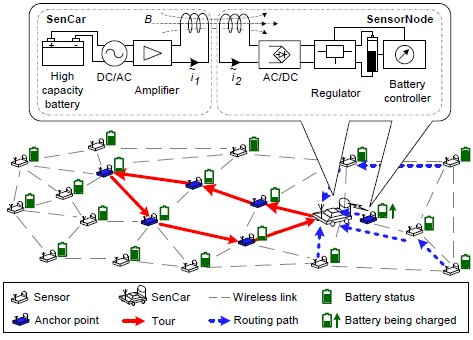
\includegraphics[width=0.6\textwidth]{images/sencar_example.jpg}
	\caption{Ένα παράδειγμα ενός ασύρματα επαναφορτιζόμενο δικτύου αισθητήρων (εξαγμένο από το \cite{yuanyuan_joint}).}
	\label{fig:wrsn_example}
\end{figure}

%4th chapter


\chapter{Ορισμός του Προβλήματος και Στρατηγικές Επίλυσης} \label{ch:strategies_solution}
Στο κεφάλαιο αυτό, θα παρουσιαστεί το μοντέλο κάτω από το οποίο γίνονται οι υπολογισμοί και αφού οριστεί το πρόβλημα με μαθηματικούς ορισμούς, θα αποδειχθεί οτι το
πρόβλημα ανήκει στην κλάση NP-πλήρης (NP-Complete) των προβλημάτων, δηλαδή δεν υπάρχει πολυωνιμικός αλγόριθμος που να το λύνει. Θα αποδειχθεί ένα άνω φράγμα του
προβλήματος βασισμένο στον γραμμικό προγραμματισμό (linear programming) ενώ θα παρουσιαστούν παρόμοιες εργασίες οι οποίες όμως μέχρι τώρα διαφέρουν ως προς την
προσέγγιση του προβλήματος σε σχέση με την παρούσα εργασία. Τέλος θα προταθούν ευρετικές στρατηγικές που αυξάνουν την απόδοση του φορτιστή αλλά και ευρετικοί
αλγόριθμοι τοπικής και καθολικής γνώσης οι οποίοι θα συγκριθούν με έναν προσαρμοστικός αλγόριθμο ο οποίος ρυθμίζει την διαδρομή του φορτιστή ανάλογα με την κατάσταση
του δικτύου.


\section{Γενικευμένος Ορισμός, Μοντέλο Επίλυσης και Ιδιότητες}
Στην ενότητα αυτή παρουσιάζεται ο γενικευμένος ορισμός του προβλήματος ο οποίος δεν αφορά μόνο την τεχνολογία ασύρματης μετάδοσης ενέργειας. Αντίθετα το πρόβλημα
ορίζεται κάτω από την γενικότερη έννοια της επαναφόρτισης των κόμβων, είτε αυτή είναι ασύρματη, είτε είναι ενσύρματη. Επίσης, ορίζεται αυστηρά το μοντέλο κάτω από το
οποίο θα παρουσιαστούν οι λύσεις του προβλήματος. Είναι σημαντικό το μοντέλο να είναι απλό ώστε να είναι εύκολα δυνατό να γίνουν αναλύσεις και να εξαχθούν λύσεις
αλλά θα πρέπει ταυτόχρονα το μοντέλο να αντικατοπτρίζει την πραγματικότητα, δηλαδή να έχει άμεση σχέση με το φυσικό περιβάλλον. Στην συνέχεια αποδεικνύεται οτι το
πρόβλημα αυτό ανήκει στην κλάση των προβλημάτων που είναι NP-πλήρη (NP-complete), δηλαδή είναι υπολογιστικά δύσκολο να βρεθεί γρήγορα μια λύση.

\subsection{Γενικευμένος Ορισμός}
Οι καινούργιες τεχνολογίες που αναλύθηκαν στην ενότητα $\ref{sc:recharg_tecnhiques}$ οδηγούν σε νέες ερευνητικές προκλήσεις των ασύρματων δικτύων αισθητήρων. Ο πλέον
μεγάλος περιορισμός των υπάρχοντων τεχνολογιών είναι εκείνος της περιορισμένης ενέργειας. Όμως, με τις πρόσφατες εξελίξεις στην τεχνολογία της ασύρματης μετάδοσης
ενέργειας, ο διαχειρισμός της ενέργειας σε τέτοιου είδους δίκτυα είναι σημαντικός. Μια αποδοτική διαχείρηση ενέργειας μπορεί να οδηγήσει σε καλύτερα αποτελέσματα ως
προς όλες τις μετρικές των ΑΔΑ (ενότητα $\ref{sc:wsn_design}$). Επίσης αυτή η διαχείρηση ενέργειας στα ΑΕΔΑ θα πρέπει γίνεται παθητικά ως προς τους στατικούς κόμβους,
δηλαδή δεν χρειάζεται καινούργιο πολύπλοκο πρωτόκολο γι'αυτή την διαχείρηση που να καταναλώνει επιπλέον ενέργεια στους στατικούς κόμβους, ενώ ταυτόχρονα ιδανικά θα
πρέπει να είναι και ανεξαρτήτου του πρωτοκόλου δρομολόγησης που χρησιμοποιείται. Ο γενικευμένος ορισμός του προβλήματος παρουσιάζεται στην συνέχεια:

\textbf{Το Πρόβλημα:} \textit{Έστω ένα ασύρματα επαναφορτιζόμενο δίκτυο αισθητήρων το οποίο αποτελείται από ένα σύνολο στατικών κόμβων και έναν ειδικό κινητό κόμβο,
τον κινητό φορτιστή. Οι στατικοί κόμβοι τοποθετούνται ομοιόμορφα κατανεμημένα στην περιοχή του δικτύου και διαδίδουν τα δεδομένα τους, σύμφωνα με ένα πρωτόκολλο
δρομολόγησης, προς την Πηγή, η οποία βρίσκεται στο κέντρο του δικτύου. Ο κινητός φορτιστής έχει πεπερασμένους πόρους ενέργειας οι οποίοι όμως είναι σημαντικά
μεγαλύτεροι από τους πεπερασμένους πόρους ενέργειας των στατικών κόμβων ενώ ταυτόχρονα είναι ικανός να φορτίζει τους φορτίζει. Το πρόβλημα που μελετάται είναι ο
προσδιορισμός της βέλτιστης δυνατής διαμόρφωσης όλων των παραμέτρων του δικτύου έτσι ώστε να βελτιωθεί η απόδοτικότητα και να αυξηθεί ο χρόνος ζωής του δικτύου.}

\textit{Οι παράμετροι που θα μελετηθούν είναι η πολιτική φόρτισης του κάθε στατικού κόμβου (δηλαδή αν ο κινητός φορτιστής τον φορτίζει ολικώς ή μερικώς), η αναλογία
της ενέργειας που είναι αρχικά διαθέσιμη στον κινητό φορτιστή και στους στατικούς κόμβους, καθώς και οι βέλτιστες διαδρομές που θα ακολουθεί ο κινητός φορτιστής ως
προς την απόδοση και την αύξηση του χρόνου ζωής του δικτύου.}



\subsection{Μοντέλο Ανάπτυξης, Ενέργειας και Φόρτισης Κόμβων}
Το μοντέλο του προβλήματος, από τον ορισμό του, περιέχει 3 τύπους συσκευών. Υπάρχουν $N$ στατικοί κόμβοι (αισθητήρες) ομοιόμορφα κατανεμημένοι στο δίκτυο οι
οποίοι επιβλέπουν το περιβάλλον και ανιχνεύουν διάφορα γεγονότα που γίνονται σε αυτό. Οι στατικοί κόμβοι έχουν αρκετή υπολογιστική ισχύ για να εκτελέσουν βασικές
εφαρμογές των ασύρματων δικτύων αισθητήρων αλλά ταυτόχρονα έχουν περιορισμένους πόρους όσον αφορά την αποθήκευση της ενέργειας. Στην συνέχεια υπάρχει ένας κινητός
κόμβος, ο κινητός φορτιστής $MC$, ο οποίος θεωρούμε οτι έχει και αυτός πεπερασμένη διαθέσιμη ενέργεια αλλά πολύ μεγαλύτερη από αυτή που έχουν οι στατικοί κόμβοι.
Τέλος υπάρχει η Πηγή $S$, η οποία βρίσκεται στο κέντρο του δικτύου και είναι ο κόμβος στον οποίο καταλήγουν όλα τα πακέτα των στατικών κόμβων. Θεωρούμε οτι η Πηγή
έχει άπειρα υπολογιστική ισχύ και άπειρη ενέργεια. Επίσης θεωρείται οτι το δίκτυο είναι ένας κυκλικός δίσκος ακτίνας $R$. Η ακτίνα επικοινωνίας των κόμβων, έστω $r$
ποικίλει ανάλογα με το πρωτόκολλο δρομολόγησης που χρησιμοποιείται. Η πυκνότητα του δικτύου είναι:
\begin{align*}
\rho = \frac{N}{\pi\cdot R^{2}}
\end{align*}

Στο μοντέλο ο κινητός φορτιστής $MC$ δεν συλλέγει δεδομένα από τους κόμβους αλλά μόνο τους φορτίζει. Επίσης χάρην απλότητας θεωρείται οτι όλοι οι
κόμβοι έχουν την ίδια συχνότητα παραγωγής μηνυμάτων, έστω $\lambda$ πακέτα ανά μονάδα χρόνου. Επιπλέον Θεωρείται οτι $E_{total}$ είναι η συνολική διαθέσιμη ενέργεια
που μπορούμε να βάλουμε στο δίκτυο, είτε δοθεί όλη στους στατικούς κόμβους είτε την μοιράστεί ανάμεσα στους στατικούς κόμβους και τον κινητό φορτιστή. Δηλαδή
αρχικά είναι:
\begin{align}
\label{total}
E_{total} = E_{sensors} + E_{MC}^{init}
\end{align}
όπου $E_{sensors}$ είναι η αρχική ενέργεια που δίνεται στους στατικούς κόμβους και $E_{MC}^{init}$ η αρχική ενέργεια που δίνεται στον κινητό φορτιστή. Η μέγιστη
ενέργεια που μπορεί να αποθηκεύσει ένας στατικός κόμβος είναι:
\begin{align*}
E^{max}_{sensor} = \frac{E_{sensors}}{N}
\end{align*}
Επομένως έχουμε:
\begin{align*}
E_{total} = N \cdot E^{max}_{sensor} + E_{MC}^{init}
\end{align*}
Αν διαιρέσουμε με $E_{total}$ τότε έχουμε:
\begin{align*}
Per_{sensors} + Per_{MC}^{init} = 1
\end{align*}
όπου $Per_{sensors}$ και $Per_{MC}^{init}$ είναι τα ποσοστά ενέργειας ως προς την συνολική αρχική ενέργεια των στατικών κόμβων και του κινητού φορτιστή αντίστοιχα.
Σε κάθε χρονική στιγμή η εναπομείνουσα ενέργεια που υπάρχει στον κινητό φορτιστή είναι $E^{curr}_{MC}$.

Για την μετάδοση και λήψη ενός μηνύματος θεωρείται οτι το κύκλωμα καταναλώνει ενέργεια αντίστοιχα με το μέγεθος του μηνύματος. Έτσι, αν πρέπει να μεταδοθεί ένα
μήνυμα με $κ$ bits τότε ο πομπός καταναλώνει ενέργεια $E_{\tau}(k) = \epsilon_{trans}\cdot k$ όπου $\epsilon_{trans}$ είναι η ενέργεια που
χρειάζεται το κύκλωμα για να δουλέψει και εξαρτάται από την απόσταση. Συνήθως η δύναμη που χρειάζεται για να μεταδοθεί ένα μήνυμα σε απόσταση $d$ από τον πομπό είναι
περίπου $d^{\alpha}$ όπου $2\leq\alpha\leq6$ είναι μια σταθερά. Χαρην απλότητας εδώ θεωρείται οτι $\alpha = 2$. Επίσης για να ληφθεί ένα μήνυμα πάλι με $k$ bits ο
δέκτης καταναλώνει ενέργεια ίση με $E_{R}(k) = \epsilon_{recv}\cdot k$ όπου $epsilon_{recv}$ είναι σταθερά και είναι η ενέργεια που χρειάζεται το κύκλωμα για να
αποκωδικοποιήσει το μήνυμα.

Επίσης στο μοντέλο θεωρείται οτι η φόρτιση γίνεται σημείο με σημείο (point-to-point), δηλαδή μόνο ένας κόμβος μπορεί να φορτιστεί κάθε χρονική στιγμή από τον κινητό
φορτιστή. Για να γίνει αυτό, ο κινητός φορτιστής $MC$ πλησιάζει τον κάθε κόμβο σε πολύ κοντινή απόσταση έτσι ώστε η απόδοση της φόρτισης (είτε είναι ασύρματη είτε
είναι με φυσική επαφή) να φτάσει στο μέγιστο. Αν και για την ασύρματη φόρτιση η απόδοση της τεχνολογίας που χρησιμοποιείται δεν έχει φτάσει στο 99\%, στο μοντέλο
θεωρείται οτι η μετάφορά ενέργειας γίνεται χωρίς απώλειες χάρην απλότητας. Ο χρόνος που διαρκεί καθώς ο κινητός κόμβος κινείται από στατικό κόμβο σε στατικό κόμβο,
θεωρείται πολύ μικρός συγκρινόμενος με τον χρόνο που χρειάζεται για να φορτιστεί ένας στατικός κόμβος. Τέλος στο μοντέλο θεωρείται οτι ο χρόνος που χρειάζεται για να
φορτιστεί πλήρως ένας στατικός κόμβος από τον κινητό φορτιστεί είναι ίσος για όλους τους στατικούς κόμβους και ανεξάρτητος από την ενέργειά του εκείνη την χρονική
στιγμή.


\subsection{NP-πληρότητα του Προβλήματος}
Για να δείχθεί οτι το πρόβλημα είναι NP-πλήρες (NP-Complete), δηλαδή υπολογιστικά δύσκολο να λυθεί, θα εξάγουμε από τον ορισμό του αρχικού προβλήματος τον ορισμό του
αντίστοιχου προβλήματος απόφασης, το πρόβλημα δρομολόγησης του κινητού φορτιστή  (Charger Dispatch Dicision Problem - CDDP), το οποίο και παρουσιάζεται παρακάτω.

\begin{definition}
(CDDP) Έστω οτι δίνεται ένα σύνολο $S$ κόμβων όπου ο καθένας έχει την δυνατότητα να αποθηκεύσει $E$ μονάδες ενέργειας και για κάθε κόμβο $s\in S$ μια λίστα από
ζευγάρια $(t_{s}^{j}, e_{s}^{j}),\; j\geq 1$ στην οποία $t_{s}^{j}$ αντιστοιχεί στην χρονική στιγμή κατα την οποία το μήνυμα $j$ του $s$ δημιουργήθηκε και $e^{j}_{s}$
είναι η ενέργεια που χρησιμοποίησε ο κόμβος $s$ για να το μεταδόσει. Δίνεται επίσης ένα μητρώο $D\in R^{|S|\times |S|}$ όπου $D_{i,j}$ είναι η απόσταση μεταξύ των
κόμβων $i$ και $j$, και ένας κινητός φορτιστής $M$ ο οποίος μπορεί να φορτίσει έναν κόμβο στην αρχική του ενέργεια σε μια χρονική μονάδα. Το πρόβλημα απόφασης του
φορτιστή είναι να  καθοριστεί αν υπάρχει εφικτή διαδρομή του φορτιστή $M$ που να επισκέπτεται τους κόμβους έτσι όστε κανένα μήνυμα να μη χαθεί λόγω ανεπαρκειας
ενέργειας.
\end{definition}
Να σημειωθεί οτι στον ορισμό η ενέργεια που απαιτείται για την λήψη μηνυμάτων θεωρείται αμεληταία. Επίσης, τα μηνύματα τα οποία ένας στατικός κόμβος είναι δυνατόν να
λάβει από άλλους στατικούς κόμβους, συμπεριλαμβάνονται σε κάθε λίστα $L_{s}$. Επομένως θεωρείται οτι τα μηνύματα αυτά παράγονται από τον ίδιο τον κόμβο $s$. Αυτό
επιτρέπει την εξέταση διαφορετικών αλγορίθμων δρομολόγησης με έναν ενιαίο τρόπο.

Για την απόδειξη της NP-πληρότητας του προβλήματος, θα χρησιμοποιήθεί ένα ήδη γνωστό NP-πλήρες πρόβλημα, τον γεωμετρικά περιοδεύων πωλητή. Ο ορισμός του προβλήματος
όπως παρουσιάζεται στο \cite{Garey_Johnson} (σελίδα 212) είναι ο εξής:
\begin{definition}
\label{G-TSP} 
Έστω $P \subseteq \mathbb{Z} \times \mathbb{Z}$ ένα σύνολο σημείων στο δισδιάστατο χώρο και $B$ ένας θετικός ακέραιος αριθμός.
Υπάρχει διαδρομή μήκους μικρότερου ή ίσου του $B$ για το πρόβλημα του περιοδεύοντος πωλητή με τις συντεταγμένες των πόλεων να ισχύει $C=P$ και η απόσταση
$d((x_{1},y_{1}),(x_{2},y_{2}))$ να είναι ίση με την διακριτή ευκλείδια απόσταση δηλαδή
\begin{align*}
d((x_{1},y_{1}),(x_{2},y_{2})) = [\sqrt{(x_{2}-x_{1})^{2} + (Y_{2}-y_{1})^{2})}]
\end{align*}
\end{definition}
Στο \cite{PapadimitriouNP} αποδεικνύεται οτι το πρόβλημα του γεωμετρικά περιοδεύοντος πωλητή είναι NP-πλήρες.
\begin{theorem}\label{th:np-complete}
Το πρόβλημα CDDP είναι NP-Complete
\end{theorem}
\begin{proof}
Είναι εύκολο να παρατηρηθεί οτι δεδομένου μιας συγκεκριμένης διαδρομής $W$ του φορτιστή $MC$ που επισκέπτεται τους κόμβους του συνόλου $S$, είναι πολύ εύκολο να
πιστοποιηθεί αν αυτή η διαδρομή είναι ικανή έτσι ώστε κανένα μήνυμα να μη χαθεί, δηλαδή κανένα μήνυμα $x$ το οποίο γεννήθηκε στον κόμβο $s$ έτσι ώστε $x$ είναι το
$j$-στό μήνυμα του κόμβου $s$ και ο κόμβος αυτός έχει λιγότερη διαθέσιμη ενέργεια από $e^{j}_{s}$ την χρονική στιγμή $t^{j}_{s}$. Προκειμένου να ελεγθεί αν το μήνυμα
$x$ χάθηκε στον κόμβο $s$ αρκεί να επαληθεύθεί οτι ο φορτιστής επισκέφθηκε τον κόμβο $s$ στο χρονικό διάστημα $[d_s^j, t_s^j]$, όπου
\begin{align*}
d_s^j = \inf_t\left\{ \sum_{i: t < t_s^i \leq t_s^j} e_s^{i} \leq E \right\}
\end{align*}
Συγκεκριμένα, αυτό μπορεί να γίνει σε $O(T \cdot |W|)$ χρόνο όπου $T$ είναι ο συνολικός αριθμός γεγονότων που δημιουργήθηκαν στο δίκτυο. Επομένως CDDP $\in$ NP.

Για δεύτερο μέρος της απόδειξης θα χρησιμοποιηθεί το G-TSP που δίνεται στον Ορισμό~\ref{G-TSP}. Έστω $P \subseteq \mathbb{Z} \times \mathbb{Z}$ και $Β\in
\mathbb{N}$ η είσοδος του προβλήματος G-TSP. Η μετατροπή αυτής της εισόδου σε είσοδο για το CDDP θα γίνει ως εξής: χρησιμοποιείται ένα σύνολο $S$ των $|S|=|P|$
κόμβων και η απόσταση $D_{i,j}$ είναι ίση με την Ευκλίδεια απόσταση μεταξή του $i$-οστού και $j$-οστού σημείου στο $P$. Επιπλέον, για κάθε κόμβο $s\in S$
ορίζεται η λίστα των γεγονότων του να είναι $L_{s} = \{(0, E), (\frac{B}{v}, 1)\}$, όπου $v$ είναι η ταχύτητα του φορτιστή. Δηλαδή, 2 γεγονότα συμβαίνουν σε κάθε
κόμβο $s$, συγκεκριμένα ένα την χρονική στιγμή 0 εξαντλώντας όλη την διαθέσιμη ενέργεια κάθε κόμβου και ένα γεγνονός την χρονική στιγμή $\frac{B}{v}$ το οποίο
απαιτεί ενέργεια 1. Μια λύση σε αυτό το στιγμιότυπο του CDDP θα μπορούσε να δώσει μία λύση για το G-TSP, το οπίο σημαίνει οτι G-TSP$\leq_{m}$CDDP. Αυτό ολοκληρώνει
την απόδειξη.
\end{proof}
\subsection{Ένα Άνω Φράγμα}

\section{Σχετική Έρευνα}
Η πρώτη εργασία που μελετάει την περίπτωση επαναφόρτισης των κόμβων του δικτύου μέσα από διάφορες πηγές ενέργειας δημοσιεύτηκε το 2003 \cite{estrin_recharge}, πολύ
πριν αναπτυχθεί η τεχνολογία της ασύρματης μεταφοράς ενέργειας. Οι πηγές ενέργειας που χρησιμοποιούνται δεν κατονομάζονται αλλά ορίζονται τα βασικά θεμέλεια για να
είναι το δίκτυο ικανό να λειτουργεί για πάντα. Συγκεκριμένα, η εργασία αναλύει την περίπτωση όπου υπάρχουν στατικοί κόμβοι στο δίκτυο και μερικοί κινητοί κόμβοι οι
οποίοι συνέχεια ψάχνουν για διαθέσιμη ενέργεια στην περιοχή του δικτύου και την παραδίδουν στους στατικούς κόμβους.
Συγκεκριμένα σε κάθε στιγμή η ενέργεια που καταναλώνεται σε έναν κόμβο $i$ ορίζεται ως
\begin{align*}
E(i,t)=\int^{t}_{t_{0}}[P_{p}(i,t)-P_{c}(i,t)]dt
\end{align*}
όπου $P_{p}(i,t)$ είναι η πρόσθεση ενέργειας του κόμβου και $P_{c}(i,t)$ είναι η κατανάλωση ενέργειας του κόμβου την ίδια χρονική στιγμή. Για το δίκτυο το άθροισμα
των διαφορετικών ενεργειών των κόμβων θα είναι
\begin{align*}
E(t)=\int^{t}_{t_{0}}(\sum\limits_{\substack{i}}[P_{p}(i,t)-P_{c}(i,t)])dt
\end{align*}
Ένας κόμβος ορίζεται ως αυτοδύναμος (self-contained) αν $E(i,t)>0 \forall t>0$ ενώ ένα δίκτυο ορίζεται ως αυτοδύμαο αν $E(t)-E_{overhead}>0\forall t>0$ όπου 
$E_{overhead}$ είναι η κατανάλωση ενέργεια που προκύπτει από την εκτέλεση των διαφόρων αλγορίθμων στο δίκτυο. Η εργασία καταλήγει με ένα πρότυπο σύστημα που
επαναφορτίζει τους κόμβους.

Η εργασία στο \cite{smart_dust_revisited} περιγράφει τον τρόπο με τον οποίο θα πρέπει να ενσωματωθεί αυτή η νέα τεχνολογία στα δίκτυα ασύρματων αισθητήρων.
Συγκεκριμένα περιγράφει εφαρμογές οι οποίες είναι κατάλληλες για ασύρματα επαναφορτιζόμενα δίκτυα αισθητήρων, ο τρόπος προσέγγισής τους, τα πλεονεκτήματά τους αλλά
και τα μειονεκτήματά τους σε σχέση με τα κλασσικά δίκτυα αισθητήρων. Στην εργασία \cite{optimal_scheduling} οι συγγραφείς αναλύουν το πρόβλημα της βέλτιστης
σχεδιασμό του φορτιστή αλλά και της πολιτικής ύπνου που θα πρέπει να ακολουθούν οι στατικοί κόμβοι για στοχαστική ανίχνευση γεγονότων. Επίσης αναλύεται η
μεγιστοποίηση της ποιότητας της ανίχνευσης τους.

Η εργασία \cite{prolonging_j-roc} εξετάζει το σενάριο όπου υπάρχουν στατικοί κόμβοι, ένας κινητός φορτιστής και μια στατική Πηγή η οποία κατευθύνει τον κινητό
φορτιστή. Η εντολές που δίνει στον φορτιστή εξαρτώνται από παράγοντες όπως η τρέχουσα ενέργεια ή ο ρυθμός κατανάλωσης ενέργειας των κόμβων οι οποίες ενσωματώνονται σε
μηνύματα δεδομένων (piggybacked). Οι συγγραφείς δείχνουν οτι το πρόβλημα είναι NP-πλήρες μέσω αναγωγής στο ήδη γνωστό NP-πλήρες πρόβλημα του περιοδεύοντος πωλητή
(TSP). Στην συνέχεια κατασκευάζουν 2 greedy αλγορίθμους οι οποίοι προσπαθούν να λύσουν αποδοτικά το πρόβλημα της διαχείρησης της ενέργειας του κινητού φορτιστή και
εφαρμόζουν προσομοιώσεις αλλά και πειραματικές εξομοιώσεις με πραγματικά συστήματα.

Στην εργασία \cite{immortal_wsns} οι συγγραφείς εξετάζουν το σενάριο στο οποίο υπάρχουν στατικοί κόμβοι οι οποίοι ανιχνεύουν το περιβάλλον, μία στατική Πηγή στην
οποία καταλήγουν όλα τα πακέτα και ένας κινητός φορτιστής ο οποίος έχει πεπερασμένη ενέργεια, αλλά πολύ μεγαλύτερη από αυτή των στατικών κόμβων και έχει την
δυνατότητα να τους φορτίζει. Επίσης θεωρείται οτι ο κινητός μόλις του τελειώσει η ενέργεια θα πρέπει να επιστρέψει σε συγκεκριμένο σημείο στο οποίο θα γίνει η
αντικατάσταση της μπαταρίας του. Στην εργασία αποδεικνύονται κάτω από τις προυποθέσεις του μοντέλου οι απαραίτητες αλλά και αναγκαίες συνθήκες που θα πρέπει να
ισχύουν προκειμένου οι κόμβοι να είναι αθάνατοι, δηλαδή ο κινητός φορτιστής να προλαβαίνει πάντα να τους φορτίζει. Επίσης αποδεικνύεται οτι η διαδρομή του κινητού
φορτιστή θα πρέπει να είναι ο μικρότερος Χαμιλτονιανός κύκλος.

Η εργασία στο \cite{j-roc} εξετάζει ένα παρόμοιο σενάριο. Στο δίκτυο υπάρχουν στατικοί κόμβοι οι οποίοι επιβλέπουν και ανιχνεύουν γεγονότα, υπάρχει ένας κινητός
φορτιστής ο οποίος μόνο φορτίζει τους κόμβους, δηλαδή δεν συλλέγει δεδομένα από τους κόμβους, και μία στατική Πηγή στην οποία καταλήγουν όλα τα μηνύματα των στατικών
κόμβων, μέσω πολυ-βηματικών (multi-hop) μεταδόσεων. Το πρωτόκολλο δρομολόγησης που χρησιμοποιείται από τους στατικούς κόμβους είναι το Collection Tree Protocol (CTP)
μια μορφή greedy πρωτοκόλλου που όμως βασίζεται σε δενδρική μορφή. Εδώ ο χρόνος χωρίζεται σε γύρους όπου ο κάθε γύρος είναι αρκετά μεγάλος σε σχέση με τον χρόνο
αναφοράς δεδομένων των στατικών κόμβων. Ο αλγόριθμος που βρίσκει την διαδρομή που θα ακολουθήσει ο κινητός φορτιστής εφαρμόζεται σε 2 βήματα. Αρχικά ο κινητός
φορτιστής βρίσκει ποιούς κόμβους θα φορτίσει, δηλαδή θα συμπεριλάβει στην διαδρομή του. Τα σημεία αυτά εξαρτώνται από πολλούς παράγοντες όπως ο ρυθμός κατανάλωσης της
ενέργειας, η εναπομείνουσα ενέργεια, ο ρυθμός γέννησης μηνυμάτων κλπ των στατικών κόμβων ή υποπεριοχών του δικτύου. Στην συνέχεια ο φορτιστής εφαρμόζει έναν ήδη
γνωστό αλγόριθμο \cite{VRPTW_solver} για δρομολόγηση οχημάτων με χρονικά παράθυρα έτσι ώστε να υπάρχει ελαχιστοποίηση της μηχανικής ενέργειας.

Όπως προκύπτει από την ανάλυση ο φορτιστής φορτίζει ουσιαστικά τα πιο κρίσιμα μονοπάτια του δικτύου, δηλαδή τα μονοπάτια από τα οποία περνάνε τα περισσότερα δεδομένα
των στατικών κόμβων και επομένως υπάρχει πολύ μεγάλη κατανάλωση ενέργειας. Οι συγγραφείς εκτέλεσαν εξομοιώσεις οι οποίες σείχνουν οτι υπάρχει μεγάλη χρονική επέκταση
της ζωής του δικτύου.


Στην εργασία \cite{yuanyuan_joint} εξετάζεται το σενάριο κατα το οποίο χρησιμοποιείται μια κινητή οντότητα (senCar) η οποία έχει την δυνατότητα να φορτίζει τους
στατικούς κόμβους του δικτύου αλλά ταυτόχρονα αυτή η οντότητα λειτουργεί ως Πηγή για το δίκτυο. Δηλαδή καθώς κινείται μέσα στο δίκτυο, αυτή η κινητή οντότητα
παραδίδει ενέργεια σε όσους κόμβους την χρειάζονται και συλλέγει τα δεδομένα από τους κόμβους. Οι συγγραφείς της εργασίας προσπαθούν να βελτιστοποιήσουν την τροχιά
της κινητής οντότητας με σε περιορισμούς που υπόκεινται στην αποδοτική διαχείρηση της ενέργειας αλλά και την αποδοτική συλλογή των δεδομένων από τους στατικούς
κόμβους. Ο χρόνος στο μοντέλο χωρίζεται σε γύρους μήκους $T$ τους οποίους η κινητή οντότητα εφαρμόζει μια λύση η οποία αποτελείται από 2 βήματα: Αρχικά βρίσκει όλα
εκείνα τα σημεία που θα πρέπει να επισκεφθεί κατα την διάρκεια ενός γύρου. Στην συνέχεια βρίσκει το βέλτιστο μονοπάτι που πρέπει να ακολοθήσει για να καλύψη όλα τα
σημεία και τέλος κάθε κόμβος βρίσκει το μονοπάτι μέσα από το οποίο θα στείλει στην κινητή οντότητα τα δεδομένα του.

\begin{figure}[h]
	\centering
	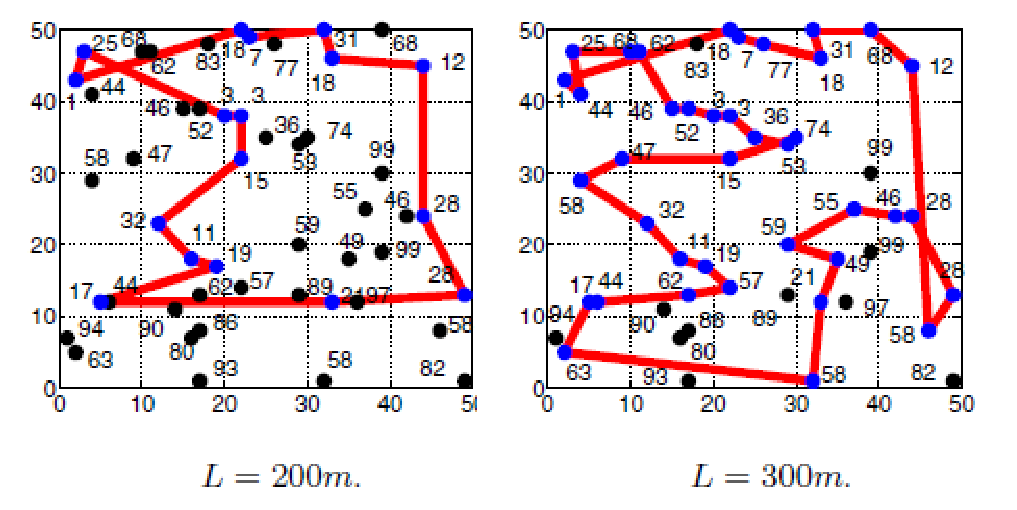
\includegraphics[width=0.8\textwidth]{images/yuanyuan_recharg_paths.eps}
	\caption{Δεξιά καλύφθηκε μεγαλύτερη διαδρομή αλλά ο κάθε κόμβος ξεχωριστά φορτίστηκε λιγότερο}
	\label{fig:yuanyuan_recharg_paths}
\end{figure}
Όπως φαίνεται και στην εικόνα \ref{fig:yuanyuan_recharg_paths} όσα περισσότερα σημεία εισαχθούν στο μονοπάτι που θα ακολουθήσει η κινητή οντότητα, τότε θα
υπάρχει μεγαλύτερη χρονοκαθυστέρηση (latency) στην συλλογή δεδομένων των στατικών κόμβων. Επομένως θα πρέπει να υπάρχει εξισορρόπηση ανάμεσα στην χρονοκαθυστέρηση και
στους κόμβους που θα φορτιστούν. Για να το πετύχουν αυτό, οι συγγραφείς απαιτούν από κάθε στατικό κόμβο να στείλει λίγο πριν το τέλος του γύρου την τρέχουσα ενέργειά
του. Αφού μαζευτούν όλες οι τρέχουσες ενέργειες των κόμβων στην κινητή οντότητα, αυτή τις διατάσει σε αύξουσα σειρά και ανάλογα με το όριο της διαδρομής επιλέγει τους
$L$ πρώτους κόμβους. Στην συνέχεια εφαρμόζεται ένας προσεγγιστικός αλγόριθμος TSP ο οποίος βρίσκει μία καλή διαδρομή για τα σημεία που επιλέχθηκαν. Για τον τρόπο
(μονοπάτι) με τον οποίο οι στατικοί κόμβοι επιλέγουν να στείλουν τα δεδομένα τους, οι συγγραφείς καταστρώνουν ένα γραμμικό πρόγραμμα το οποίο στη συνέχει το λύνουν
με έναν κατανεμημένο προσεγγιστικό αλγόριθμο. Οι προσομοιώσεις δείξαν οτι υπάρχει δραματική αυξηση του χρόνου ζωής του δικτύου σε σχέση με ασύρματα δίκτυα αισθητήρων
τα οποία χρησιμοποιούν εναλλακτικές μορφές ενέργειας.


Από τις παραπάνω δημοσιεύσεις μόνο οι \cite{prolonging_j-roc}, \cite{j-roc}, \cite{yuanyuan_joint} \cite{immortal_wsns} προσπαθήσουν να
λύσουν το πρόβλημα ενώ μόνο η \cite{yuanyuan_joint} χρησιμοποιεί κατανεμημένο αλγόριθμο αλλά  καμία από τις λύσεις που προτείνονται δεν χρησιμοποιεί τοπική
πληροφορία. Αντίθετα όλοι οι αλγόριθμοι που προτείνονται χρησιμοποιούν πληροφορίες από όλους τους κόμβους του δικτύου. Αυτό αποτελεί πρόβλημα καθώς σπαταλάται πολύ
ενέργεια σε μεγάλα δίκτυα. Επίσης δεν μελετώνται άλλα, πιο γενικά, θέματα όπως η γενική απόδοση του φορτιστή σε σχέση με την διαθέσιμη ενέργεια του δικτύου, η
αναλογία διαθέσιμης ενέργειας του φορτιστή σε σχέση με την διαθέσιμη ενέργεια των στατικών κόμβων αλλά και στρατηγικές φόρτισης που θα μπορούσαν να ωφελήσουν την
χρονοζωή (lifetime) του δικτύου.

\section{Στρατηγικές Επίλυσης}
Προκειμένου να λυθεί το CDDP πρόβλημα αποδοτικά, θα εφαρμοστούν ορισμένες στρατηγικές επίλυσης οι οποίες έχουν να κάνουν με συμβιβασμούς στην διαθέσιμη ενέργεια του
φορτιστή και των κόμβων.

\subsection{Ολική και Μερική Φόρτιση}
Κάθε φορά που ο φορτιστής $MC$ επισκέπτεται έναν κόμβο, μία αφελής στρατηγική θα ήταν να τον φορτίζει πλήρως τον κόμβο αυτό. Με αυτόν τον τρόπο ο $MC$ θα μπορούσε να
μεγιστοποιήσει τον χρόνο που χρειάζεται μέχρι να επιστρέψει στον ίδιο κόμβο και να τον ξαναφορτίσει για να μην εξαντληθεί όλη του η ενέργειά. Ωστόσο, καθώς το δίκτυο
λειτουργεί, υπάρχει κατανάλωση ενέργειας από τους κόμβους μέσα από την αποστολή μηνυμάτων αλλά και από τον ίδιο φορτιστή μέσα από την διαδικασία φόρτισης. Επομένως ο
φορτιστής θα έχει όλο και λιγότερη ενέργεια διαθέσιμη να δώσει στους κόμβους που την έχουν ανάγκη οι οποίοι με τον χρόνο θα αυξάνονται.

Μία διαφορετική στρατηγική για τον φορτιστή είναι να απλώσει συνετά την πολύτιμη ενέργειά του σε όσους περισσότερους κόμβους είναι δυνατόν προκειμένου να επεκτείνει
τον χρόνο ζωής του δικτύου. Ακολουθώντας αυτή την λογική, το ποσό της ενέργειας ο φορτιστής $MC$ παραδίδει σε έναν κόμβο είναι ανάλογο της διαθέσιμης ενέργειας του
ίδιου του φορτιστή. Δηλαδή, ο $MC$ φορτίζει έναν κόμβο μέχρι η ενέργειά του να γίνει:
\begin{align*}
e_{i} \approx \frac{E^{curr}_{MC}}{E^{init}_{MC}}\cdot E^{max}_{sensor}
\end{align*}

Προκειμένου να καθοριστεί η βέλτιστη στρατηγική φόρτισης στο κεφάλαιο \ref{ch:results} εκτελούνται μια σειρά πειραμάτων τα οποία συγκρίνουν την στρατηγική της ολικής
φόρτισης και την στρατηγική της προσαρμοστικής, μερικής φόρτισης. Τα πειραματικά αποτελέσματα δείχνουν οτι η μερική φόρτιση είναι πιο αποδοτική από την ολική φόρτιση.

\subsection{Ποσοστό Ενέργειας στον Φορτιστή}
Για να υπάρχει σωστή εκτίμηση της απόδοσης του φορτιστή, θεωρείται οτι η αρχική διαθέσιμη ενέργεια του δικτύου είναι $E_{total}$ και είναι πεπερασμένη και σταθερή
για όλες τις περιπτώσεις. Δηλαδή, λόγω του \ref{total} η $E_{total}$, ανάλογα σε κάθε περίπτωση, διαμοιράζεται ανάμεσα στον φορτιστή και τους κόμβους του δικτύου. Με
αυτόν τον τρόπο θα είναι δυνατόν να διερευνηθεί καλύτερα αν οι μετρικές του δικτύου έχουν καλύτερη απόδοση με ή χωρίς τον φορτιστή και την διαδικασία φόρτισης. Αυτός
ο συγκεκριμένος συμβιβασμός έχει σχέση με το ποσό της ενέργεια (σε σχέση με την ολική ενέργεια $E_{total}$) το οποίο θα διοχετευθεί αρχικά στον φορτιστή $MC$.
Περισσότερη ενέργεια στον φορτιστή θα οδηγήσει σε καλύτερη διαχείρηση της ενέργειας στο δίκτυο, αφού ο φορτιστής μπορεί να δώσει την ενέργεια εκεί που πραγματικά
χρειάζεται (π.χ. σε ένα κρίσιμο μονοπάτι). Ωστόσο, λόγω της \ref{total} περισσότερη ενέργεια στον $MC$ θα σήμαινε οτι οι κόμβοι ξεκινάνε στο δίκτυο με μικρότερη
αρχική ενέργεια, δηλαδή χωρίς να είναι πλήρως φορτισμένοι. Έτσι, θα είναι πολύ πιθανόν οτι θα τους τελειώσει η ενέργεια πριν ο φορτιστής $MC$ τους φορτίσει,
οδηγόντας έτσι σε πιθανές αποσυνδέσεις του δικτύου και χαμηλή κάλυψη της περιοχής από τους κόμβους.

Προκειμένου να καθοριστεί η βέλτιση κατανομή ενέργειας ανάμεσα στον φορτιστή και τους κόμβους στο κεφάλαιο \ref{ch:results} εκτελούνται μια σειρά από πειράματα με
διάφορες αναλογίες ανάμεσα στην αρχική διαθέσιμη ενέργεια των κόμβων, $E_{sensors}$ και την αρχική διαθέσιμη ενέργεια του φορτιστή, $E^{init}_{MC}$. Όπως θα φανεί στο
κεφάλαιο \ref{ch:results} η βέλτιστη αναλογία που βρέθηκε πειραματικά είναι 20\% της αρχικής ενέργειας $E_{total}$ να δοθεί στον φορτιστή και το υπόλοιπο 80\% της
ενέργειας να δοθεί στους κόμβους.

\subsection{Διαδρομές του Φορτιστή}
Η αποδοτική διαχείρηση της ενέργειας σε ένα ασύρματο δίκτυο αισθητήρων εξαρτάται σημαντικά και από τις διαδρομές που ακολουθεί ο φορτιστής. Παρακάτω παρουσιάζεται
αρχικά μια διαδρομή η οποία έχει πλήρη γνώση (global knowledge) της κατάστασης του δικτύου, 3 διαδρομες οι οποίες χρησιμοποιούν μόνο τοπική πληροφορία ενώ η
τελευταία που παρουσιάζεται όχι μόνο χρησιμοποιεί τοπική πληροφορία αλλά ταυτόχρονα έχει και προσαρμοστικό χαρακτήρα ανάλογα με την κατάσταση του δικτύου.

\subsubsection{Φορτιστής με Καθολική Γνώση}
Ο φορτιστής καθολικής γνώσης (global-knowledge charger) ο οποίο μελετάται, αποτελεί ουσιαστικά έναν αλγόριθμο άμεσης απόκρισης (online algorithm) ο οποίο σε κάθε γύρο
ελαχιστοποιεί το γινόμενο της ενέργειας του κάθε κόμβου με την απόστασή του από την τρέχουσα θέση του φορτιστή. Πιο συγκεκριμένα, σε κάθε γύρο ο φορτιστής καθολικής
γνώσεις ελαχιστοποιεί το ακόλουθο γινόμενο:
\begin{align*}
P = min\left\{ \left(1 + \frac{E_{curr}}{E_{init}}\right) \cdot \left(1  + \frac{dist_{curr}}{2R}\right) \right\}
\end{align*}
όπου $E_{curr}$, $E_{init}$  και $dist_{curr}$ είναι αντίστοιχα η τρέχουσα ενέργεια, η αρχική ενέργεια και η απόσταση του κάθε κόμβου. Η ελάχιστη τιμή λαμβάνεται
αφού γίνει η σύγκριση σε όλους τους κόμβους. Αφού η στρατηγική αυτή απαιτεί καθολική γνώση της κατάστασης του δικτύου, είναι αναμενόμενο να υπερτερεί κάθε άλλου
αλγορίθμου που χρησιμοποιεί τοπική γνώση. Ωστόσο, τέτοιοι αλγόριθμοι δεν είναι καταλληλοι για πραγματικά δίκτυα και δεν έχει καλή κλιμακωσιμότητα καθώς εισάγει
πολύ μεγάλο επικοινωνιακό κόστος αφού κάθε κόμβος θα πρέπει να διαδόσει την τρέχουσα ενέργειά του σε κάθε γύρο.


\subsubsection{Σπειροειδης Φορτιστής}
Ο σπειροειδης φορτιστής ξεκινάει από την Πηγή και διανύει διαδρομή η οποία σχηματίζει ομόκεντρους κύκλους με κέντρο την Πηγή αλλά με αυξανόμενη ακτίνα. Επομένως
σχηματίζει μία σπείρα μέχρις ότου φτάσει τα ακριανά όρια της περιοχής του δικτύου. Στην συνέχεια  ο $MC$ ακολουθεί την ίδια διαδρομή αλλά με αντίθετη κατεύθυνση. Τα
πλεονεκτήματα αυτής της κίνησης είναι οτι η σπείρα είναι ο μόνος ντεντερμινιστικός αλγόριθμος ο οποίος μπορεί να καλύψει όλο το δίκτυο δίκαια, δηλαδή σχεδόν όλοι οι
κόμβοι φορτίζονται από τον $MC$ μέχρι να τελειώσει η διαθέσιμη ενέργειά του. Όμως, αυτή η κίνηση δεν είναι προσαρμοστική, δηλαδή δεν  λαμβάνει υπόψην διαφορές στον
ρυθμό κατανάλωσης των κόμβων οι οποίες προκλήθηκαν από το εκάστοτε πρωτόκολλο δρομολόγησης που τρέχει.

\subsubsection{Διαμετρικός Φορτιστής}
Ο διαμετρικός φορτιστής αρχικά ξεκινάει από την Πηγή και επιλέγει τυχαία μια κατεύθυνση την οποία ακολουθεί μέχρι να φτάσει στα όρια της περιοχής του δικτύου, δηλαδή
κινείται πάνω στην αντίστοιχη διάμετρο του δικτύου. Στην συνέχεια αφού έχει φτάσει στην περίμετρο του δικτύου, κινείται πάνω στην περίμετρο της περιοχής του δικτύου
για $d$ μοίρες, δηλαδή διανύει απόσταση ίση με $\frac{d}{2\pi}2\pi R = d\cdot R$ επάνω στην περίμετρο. Στην συνέχεια ξεκινάει να κινείται επάνω στην αντίστοιχη
διάμετρο του δικτύου εως ότου φτάσει στην αντιδιαμετρική άκρη του δικτύου. Αυτή η διαδικασία συνεχίζεται μέχρι να τελειώσει η εναπομείνουσα ενέργεια του φορτιστή.
Προκειμένου οι διαδρομές που ακολουθεί ο φορτιστής να μην επικαλύπτονται, σε κάθε βήμα το $d$ επιλέγεται τυχαία ομοιόμορφα στο διάστημα $(0,90]$ μοιρών. Ακολουθώντας
αυτή την διαδρομή ο $MC$ καταφέρνει να φορτίσει όλους τους κόμβους που βρίσκονται μακριά αλλά και κοντά στην Πηγή. Ωστόσο, παρ'όλο που η διαδρομή είναι απλή, δεν
είναι προσαρμοστική. Ένα στιγμιότυπο της διαδρομής φαίνεται στην εικόνα \ref{fig:diameter_charger}.
\vspace{0.9cm}
\begin{figure}[h]
	\centering
	\includegraphics[width=0.3\textwidth]{images/diameter.eps}
	\caption{Ένα στιγμιότυπο του Διαμετρικού Φορτιστή.}
	\label{fig:diameter_charger}
\end{figure}


\subsubsection{Φορτστής σε Τυχαίο Περίπατο}
Ο φορτιστής σε τυχαίο περίπατο ακολουθεί τον τυφλό τυχαίο περίπατο (blind random walk). Σε κάθε νέο γύρο, η επόμενη κίνηση του φορτιστή είναι τυχαία, στοχαστικά
ανεξάρτητη από κάθε προηγούμενη επιλογή. Δεδομένου της τρέχουσας θέσης του φορτιστή, έστω ο κόμβος $i$ τότε η πιθανότητα μετάβασης σε οποιονδήποτε γείτονα $j$ του
κόμβου $i$ είναι $p_{i,j} =\frac{1}{deg(i)}$. Η τροχία αυτή είναι πολύ αποδοτική ως προς την έννοια οτι πιθανοτικά εγγυάται οτι τελικά όλο η περιοχή του δικτύου θα
καλυφθεί και όλοι οι κόμβοι θα επισκεφθούν Ωστόσο μπορεί να γίνει αποδοτική σε δίκτυα με περιοχές συμφόρησης ή με ειδικούς κόμβους (όπως κόμβους αρχηγούς σε
ιεραρχικά πρωτόκολλα) και γενικά σε δίκτυα που υπάρχουν κόμβοι που εξυπηρετούν μεγαλύτερη κίνηση από άλλους κόμβους όπως συμβαίνει σε πολυ-βηματικά (multi-hop)
πρωτόκολλα.

\subsubsection{Προσαρμοστικός Φορτιστής}
Δεδομένου της συμμετρίας του δικτύου, της ομοιόμορφης κατανομής, και της ομοιόμορφης γέννησης μηνυμάτων του δικτύου ο πρασαρμοστικός φορτιστής ακολουθεί μια κυκλική
τροχιά με κέντρο την Πηγή η οποία βρίσκεται στο κέντρο του δικτύου. Η ακτίνα της κυκλικής τροχιάς ποικίλει και προσαρμόζεται στην κατανάλωση ενέργειας της κάθε
υποπεριοχής του δικτύου. Έστω $S$ το σύνολο αυτών των κόμβων όπου $|S| = 2\pi R_{MC}\cdot \rho$. Έστω, επίσης, $e_{i}$ οτι δηλώνει την τρέχουσα ενέργεια του κόμβου
$i$. Ξεκινώντας από την Πηγή, ο κινητός φορτιστής διανύει μια διαδρομή η οποία σχηματίζει ομόκεντρους κύκλους με κέντρο την ίδια την Πηγή αλλά με ακτίνα η οποία
αυξάνεται ή μειώνεται ανάλογα. Σε μια δεδομένη απόσταση από την Πηγή ο προσαρμοστικός φορτιστής καταγράφει την μέση τιμή της ενέργειας των κόμβων οι οποίοι
βρίσκονται επάνω στην αντίστοιχη κυκλική τροχιά. Έστω η μέση ενέργεια όλων των κόμβων οτι είναι $\overline{E}_{current}$. Αντίστοιχα ο προσαρμοστικός φορτιστής
κρατάει στην μνήμη του την μέση τιμή της ενέργειας των κόμβων που βρίσκονταν στην προηγούμενη κυκλική τροχιά του, έστω $\overline{E}_{previous}$. Χρησιμοποιώντας
αυτές τις 2 τιμές ο προσαρμοστικός φορτιστής βελτιστοποιεί την κυκλική τροχιά του με κριτήριο την φόρτιση των κόμβων οι οποίοι καταναλώνουν την ενέργειά τους πιο
γρήγορα.

Ο αλγόριθμος που εκτελεί ο προσαρμοστικός φορτιστής φαίνεται παρακάτω:
\vspace{0.1cm}
\begin{algorithm}
\begin{algorithmic}
\caption{Προσαρμοστικός Φορτιστής}
\While{$E_{MC}^{curr} > 0$}
\State $E_{tmp}=0$
\For{every $i\in S$}
\State $E_{tmp}+=e_{i}^{c}$
\State Charge until $e_{i} \approx \frac{E_{MC}^{curr}}{E_{MC}^{init}}\cdot E_{sensor}^{max}$
\EndFor
\State $\overline{E}_{current}=\frac{E_{tmp}}{|S|} = \frac{\sum e_{i}}{|S|}$
\If {$\overline{E}_{current} \approx \overline{E}_{init}$}
    \If {$\overline{E}_{previous} \geq \overline{E}_{current}$ }
		\State	Keep direction
	\Else
		\State Change direction
	\EndIf
\EndIf
\EndWhile
\end{algorithmic}
\end{algorithm}

Ο προσαρμοστικός φορτιστής $MC$ ξεκινάει να διασχίζει το δίκτυο από το κέντρο του θέτοντας $R_{MC}=1$, δηλαδή θα επισκεφθεί όλους τους κόμβους που βρίσκονται 1-βήμα
(1-hop) μακριά από την Πηγή. Μόλις όλοι αυτοί οι κόμβοι φορτιστούν, δηλαδή οι κόμβοι που συναντά ο $MC$ έχουν ενέργεια $e_{i} = E^{max}_{sensor}$ ο $MC$ αυξάνει την
ακτίνα του $R_{MC}$ επισκέπτοντας τους κόμβους που είναι 2-βήματα (2-hop) μακριά από την Πηγή. Συγκρίνοντας τις τιμές $\overline{E}_{current}$ και
$\overline{E}_{previous}$ ο $MC$ μπορεί να καταλάβει προς ποια περιοχή θα κινηθεί, δηλαδή προς την περιοχή η οποία έχει μεγαλύτερη κατανάλωση ενέργεια. Συγκεκριμένα,
αν $\overline{E}_{current} < \overline{E}_{previous}$ τότε ο $MC$ υποθέτει οτι κινείται προς την σωστή περιοχή, δηλαδή αυτή στην οποία υπάρχει μεγάλο φορτίο.
Αντίθετα αν $\overline{E}_{current} > \overline{E}_{previous}$ τότε ο $MC$ αμέσως καταλαβαίνει οτι κινείται προς την λάθος περιοχή και έτσι αλλάζει κατεύθυνση.


%5th chapter


\chapter{Πειραματική Αξιολόγηση}\label{ch:results}
Η πειραματική αξιολόγηση έγινε στην Matlab 7.11.0. Η πηγή τοποθετήθηκε στο κέντρο (0,0) της κυκλικής περιοχής ανάπτυξης των στατικών κόμβων. Για καλύτερα στατιστικά
αποτελέσματα εφαρμόστηκε πολλές φορές η ανάπτυξη των στατικών κόμβων και κάθε πείραμα εκτελέστηκε 100 φορές. Η στατιστική ανάλυση των αποτελεσμάτων δηλώνουν
πολύ μεγάλη συγκέντρωση γύρω από την μέση τιμή, επομένως στα σχεδιαγράμματα φαίνονται μόνο οι μέσες τμές.

Για να αξιολογηθούν σωστά οι στρατηγικές και οι αλγόριθμοι που προτάθηκαν, η πειραματική αξιολόγηση γίνεται κάθε φορά σε 3 τελείως διαφορετικής φύσεως πρωτόκολλα
δρομολόγησης που όμως το καθένα αντιπροσοπεύει την αντίστοιχη οικογένεια πρωτοκόλλων δρομολόγησης. Τα πρωτόκολλα είναι το Greedy \cite{greedy_protocol}, το οποίο
ουσιαστικά αποτελεί ένα πρωτόκολλο σαν το CTP (Collection Tree Protocol) το οποίο έχει μια δενδρική μορφή, το Leach \cite{leach_protocol} το οποίο αποτελεί ένα
ιεραρχικό με συστάδες πρωτόκολλο και το $E_{i}$ \cite{debp_protocol} το οποίο αποτελεί ένα πρωτόκολλο εξισορρόπησης ενέργειας.

Αφού οι $N$ κόμβοι είναι ομοιόμορφα κατανεμημένοι σε μία κυκλική περιοχή $\mathcal{A}$ ακτίνας $R$ εφαρμόστηκε ένα γνωστό κατώφλι συνδεσιμότητας προκειμένου να
μεγιστοποιηθεί η πιθανότητα των γενημένων τυχαίων στιγμιότυπων να είναι συνδεδεμένα. Πιο συγκεκριμένα, αφού $\mathcal{A}\subset \mathbb{R}^2$, ένα στιγμιότυπο του
μοντέλου τυχαίων γεωμετρικά γραφημάτων (random geometric graphs) $\mathcal{G}(\mathcal{X}_N;r)$ κατασκευάζεται ως εξής: επιλέγονται $N$ σημεία $\mathcal{X}_N$
ομοίομορφα τυχαία στο $\mathcal{A}$. Το σύνολο $V = \mathcal{X}_N$  είναι το σύνολο των κορυφών του γράφου και δύο κορυφές συνδέονται αν οι ευκλείδιες αποστάσεις
τους είναι το πολύ $r$. Στα \cite{rg1,rg2} δείχνεται οτι το κατώφλι συνδεσιμότητας για τα $\mathcal{G}(\mathcal{X}_N;r)$ είναι $r_c = \sqrt{\frac{\ln N}{\pi N}}$. Σε
αυτή την εργασία θεωρούνται τυχαία στιγμιότυπα από $\mathcal{G}(\mathcal{X}_N;r)$ με ποικίλη πυκνότητα , επιλέγοντας $r = \sqrt{\frac{c\ln N}{\pi N}}$, για διάφορες
τιμές του $c>1$, το οποίο εγγυάται οτι το παραγόμενο τυχαίο στιγμιότυπο είναι συνδεδεμένο με μεγάλη πιθανότητα. Καθόλη την διάρκεια των πειραμάτων η παράμετρος $c$
είναι σταθερή με μεγαλύτερες τιμές για το Greedy πρωτόκολλο γιατί είναι πιο επιρρεπή σε γρηγορότερες αποσυνδέσεις.

Αφού το δίκτυο είναι αρκετά πυκνό, θεωρείται οτι κάθε μετάδοση κοστίζει $r^{2}$ σε μονάδες ενέργειας, όπου $r$ είναι ακτίνα μετάδοσης ενός κόμβου. Αφού οι κόμβοι
καθώς και η γέννηση γεγονότων είναι ομοιόμορφα κατανεμημένη, η μέση τιμή των βημάτων (hops) που χρειάζονται για ένα γεγονός να ταξιδέψει από τον πρώτο κόμβο που το
ανίχνευσε μέχρι την Πηγή είναι $\frac{R}{2}\cdot \frac{1}{r}$. Επομένως, η μέση ενέργεια που καταναλώθηκε για την δρομολόγηση ενός γεγονότος από τον πρώτο κόμβο μέχρι
την Πηγή είναι $r^2\frac{R}{2r} = \frac{rR}{2}$ και για την συνολική ενέργεια που κανατλώθηκε στο δίκτυο είναι $E_{total} = \frac{\mu r R}{2}$, όπου $\mu$ είναι ο
αριθμός των γεγονότων. Στα πειράματα δώθηκε ενέργεια ίση με $E_{total} = \frac{h\mu r R}{4}$, για $h > 1$ προκειμένου να εξασφαλιστεί οτι οι κόμβοι πεθαίνουν μετά
από αρκετούς γύρους.

Τα πειράματα επικεντρώνονται στις ακόλουθες μετρικές απόδοσης:
\begin{itemize}
\item \textbf{Ζωντανοί κόμβοι κατα την πάροδο του χρόνου}, δηλαδή ο αριθμός των κόμβων που έχουν εναπομείνουσα ενέργεια που τους καθιστά ικανούς να λειτουργούν , κατα
την διάρκεια εκτέλεσης ενός πειράματος
\item \textbf{Συνδεσιμότητα κατατ την πάροδο του χρόνου}, δηλαδή ο μέσος βαθμός (ο μέσος αριθμός γειτόνων) του κάθε κόμβου κατα την διάρκεια εκτέλεσης ενός πειράματος
\item \textbf{Χρονοκάλυψη}, δηλαδή ο μέσος αριθμός κάλυψης (coverage) του δικτύου από κόμβους 1000 τυχαίων σημείων δίκτυο κατα την πάροδο του χρόνου. Στα γραφήματα τα
χρώματα υποδηλώνουν τον αριθμό κάλυψης του σημείου σύμφωνα με την εικόνα \ref{fig:coverage_sample}.
\item \textbf{Ενεργιακός χάρτης του δικτύου}, ο οποίος είναι μια απεικόνιση του συνολικού δικτύου που εμφανίζονται οι σχετικές ενέργειες των κόμβων
\end{itemize}

\begin{figure}[h]
  \centering
  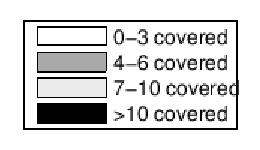
\includegraphics[width=0.3\textwidth]{images/network_coverage.eps}
  \caption{Ο μέσος αριθμός κάλυψης των σημείων σε χρώματα.}
  \label{fig:coverage_sample}
\end{figure}

Στην πειραματική αξιολόγηση ερευνούνται οι στρατηγικές που μελετήθηκαν στο κεφάλαιο \ref{ch:strategies_solution} ώστε να βρεθή η βέλτιστη στρατηγική και οι
αντίστοιχοι παράμετροι ενέργειας στους κόμβους και στον κινητό φορτιστή με κύριο στόχο την μεγιστοποίηση του χρόνου ζωής του δικτύου. Στα 3 πρώτες σειρές πειραμάτων
χρησιμοποιείται ο προσαρμοστικός φορτιστής ο οποίος διασθητικά είναι και ο καλύτερος. Στην τελευταία σειρά πειραμάτων, αφού βρεθούν οι κατάλληλες παράμετροι
κατανομής της ενέργειας για το δίκτυο, ο προσαρμοστικός φορτιστής συγκρίνεται με τους υπόλοιπους φορτιστές.

\section{Με και Χωρίς Φόρτιση}\label{sc:result1}
Η πρώτη σειρά από πειράματα αφορά την σύγκριση του δικτύου με φόρτιση και του δικτύου χωρίς φόρτιση. Όταν επιλέγεται το δίκτυο να είναι χωρίς φόρτιση τότε η συνολική
ενέργεια του δικτύου κατανέμεται όλη στους στατικούς κόμβους του δικτύου, δηλαδή ο κάθε κόμβος ξεκινάει με το 100\% της αρχικής του ενέργειας. Αντίθετα όταν
επιλέγεται το δίκτυο να είναι με φόρτιση, δηλαδή με έναν κινητό φορτιστή που φορτίζει τους κόμβους, η συνολική ενέργεια κατανέμεται ανάμεσα στους στατικούς κόμβους
και τον κινητό φορτιστή. Οι στατικοί κόμβοι σε αυτή την περίπτωση δεν ξεκινάνε με πλήρη αρχική ενέργεια αλλά με ένα ποσοστό της αρχικής ενέργειας. Στο πείραμα αυτό,
καθώς δεν έχει βρεθεί η βέλτιστη αναλογία ενέργειας ανάμεσα στον κινητό φορτιστή και τους στατικούς κόμβους, οι τελευταίοι ξεκινάνε με το με το 60\% της αρχικής τους
ενέργειας και επομένως ο φορτιστής κατέχει αρχικά το 40\% της αρχικής ολικής ενέργειας του δικτύου. Χρησιμοποιείται ο προσαρμοστικός φορτιστής. Τα αποτελέσματα των
πειραμάτων φαίνονται στις εικόνες \ref{fig:1exp_1_1}, \ref{fig:1exp_2_1}, \ref{fig:1exp_3_1}, \ref{fig:1exp_3_2}, \ref{fig:1exp_3_3}, \ref{fig:1exp_4_1},
\ref{fig:1exp_4_2} και \ref{fig:1exp_4_3}. Η διαισθητική εικόνα που αφήνουν τα αποτελέσματα είναι οτι δίνοντας ένα μέρος της συνολικής αρχικής ενέργειας του δικτύου
στον φοτιστή, ακόμα και χωρις να έχει βελτιστοποιηθεί το μέγεθος που δίνεται, υπάρχουν σημαντικά καλύτερα αποτελέσματα σε όλες τις μετρικές.



%%%%%%%%%%%%%%%%%%%%%%%%%%%% 1. LIFETIME %%%%%%%%%%%%%%%%%%%%%%%%%%%%%%%%%%%%%
\begin{figure}[H]
  \centering
  \subfloat[Greedy]{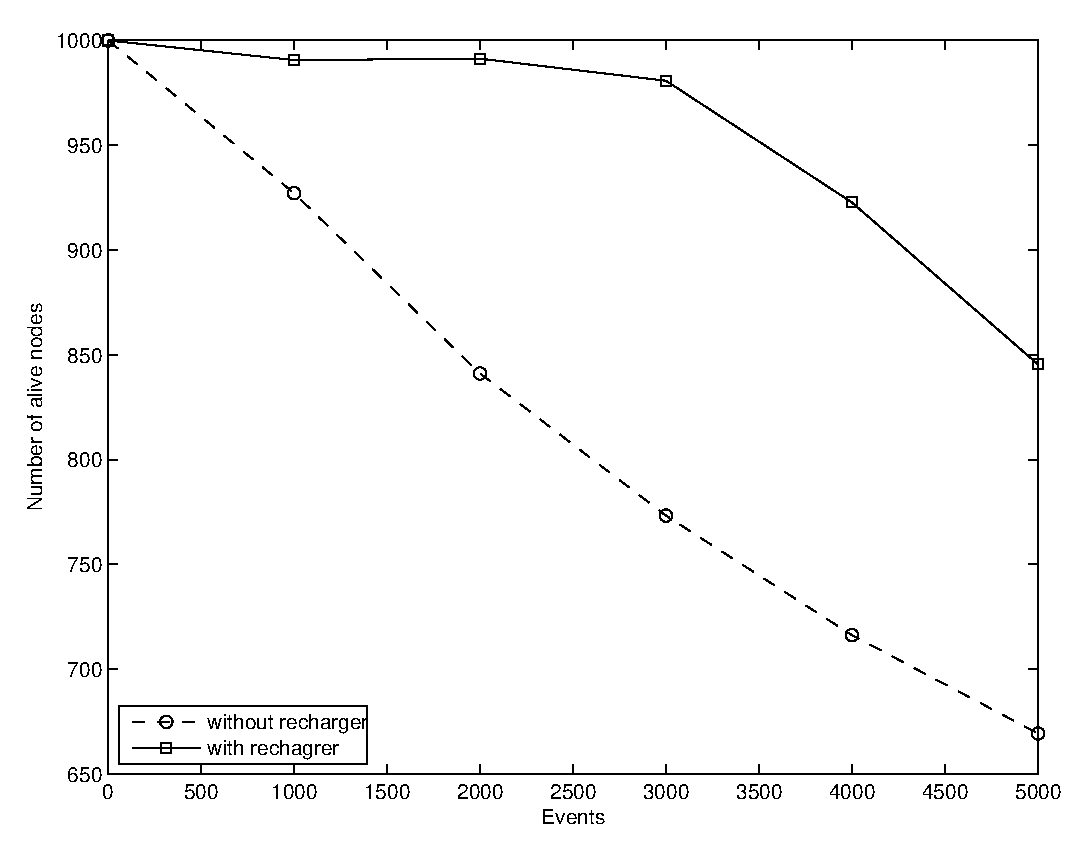
\includegraphics[width=0.32\textwidth]{experiments/classic/1.norechargeVSrecharge/alive_nodes_greedy_nonrc-rc.eps}}
  \subfloat[Leach]{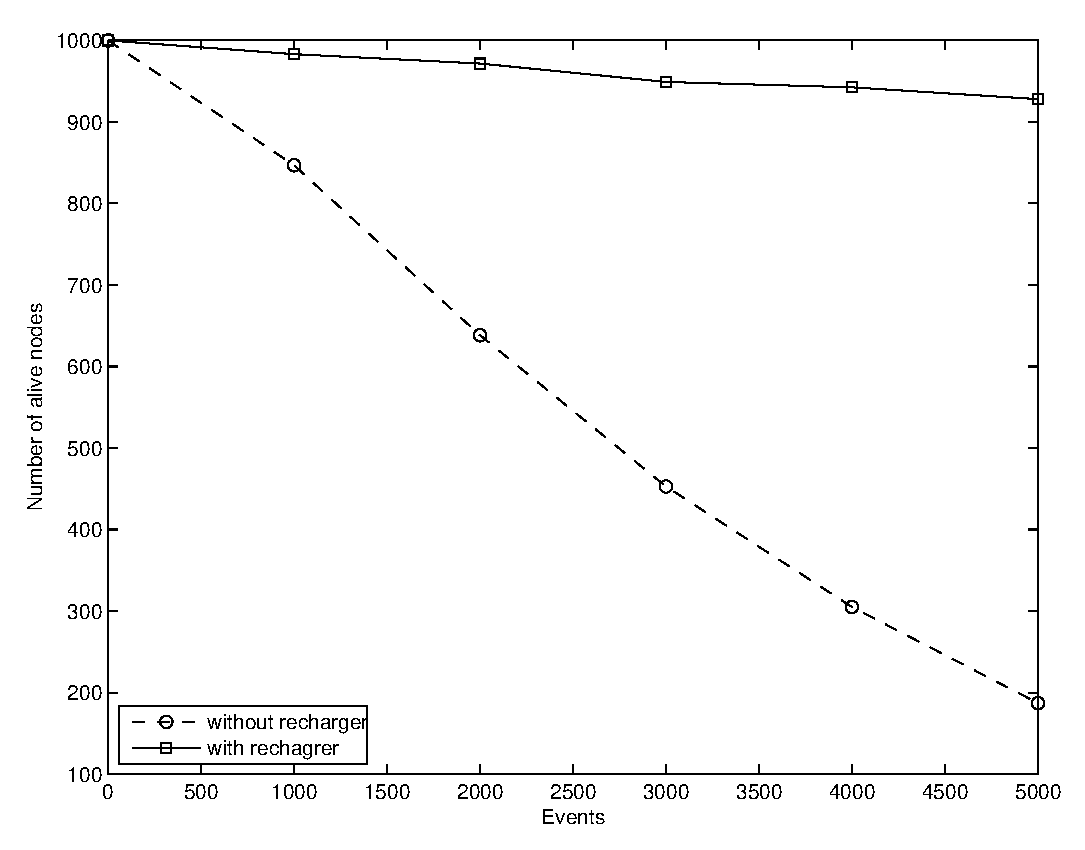
\includegraphics[width=0.32\textwidth]{experiments/classic/1.norechargeVSrecharge/alive_nodes_leach_nonrc-rc.eps}}
  \subfloat[$E_{i}$]{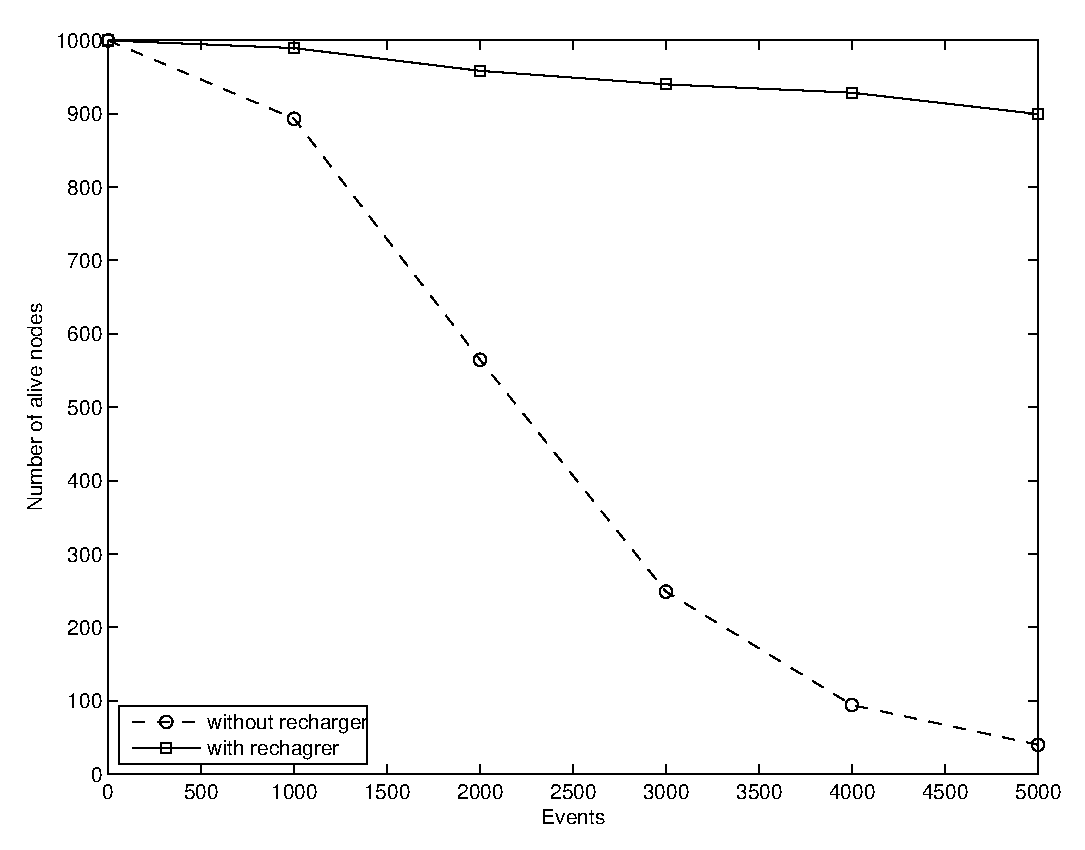
\includegraphics[width=0.32\textwidth]{experiments/classic/1.norechargeVSrecharge/alive_nodes_ei_nonrc-rc.eps}}
  \caption{Ζωντανοί κόμβοι κατά την πάροδο του χρόνου. Η συνεχόμενη γραμμή αντιστοιχεί στο δίκτυο με κινητό φορτιστή. Γίνεται εμφανές οτι υπάρχει αύξηση
	του χρόνου ζωής του δικτύου αν δοθεί μέρος της συνολικής ενέργειας
   στον φορτιστή (εδώ δόθηκε 40\%).}
  \label{fig:1exp_1_1}
\end{figure}

%%%%%%%%%%%%%%%%%%%%%%%%%%%% 2. CONNECTIVITY %%%%%%%%%%%%%%%%%%%%%%%%%%%%%%%%%%%%%
\begin{figure}[H]
  \centering
  \subfloat[Greedy]{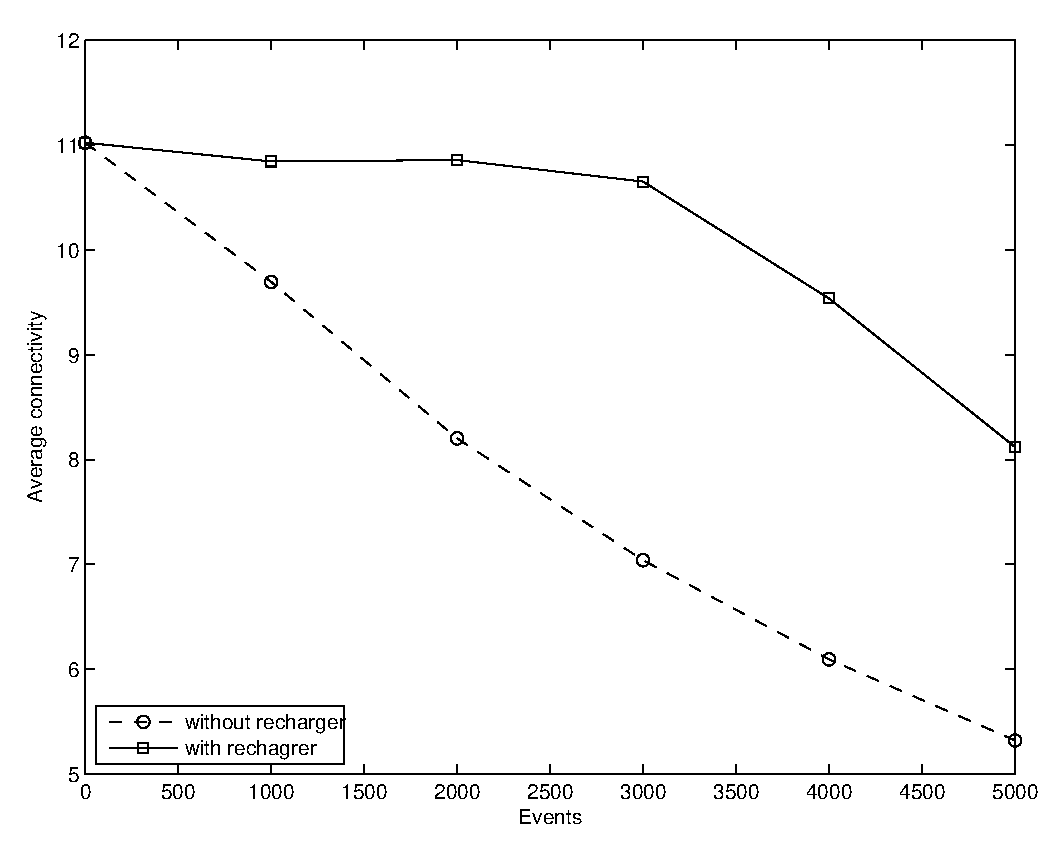
\includegraphics[width=0.32\textwidth]{experiments/classic/1.norechargeVSrecharge/connectivity_greedy_nonrc-rc.eps}}
  \subfloat[Leach]{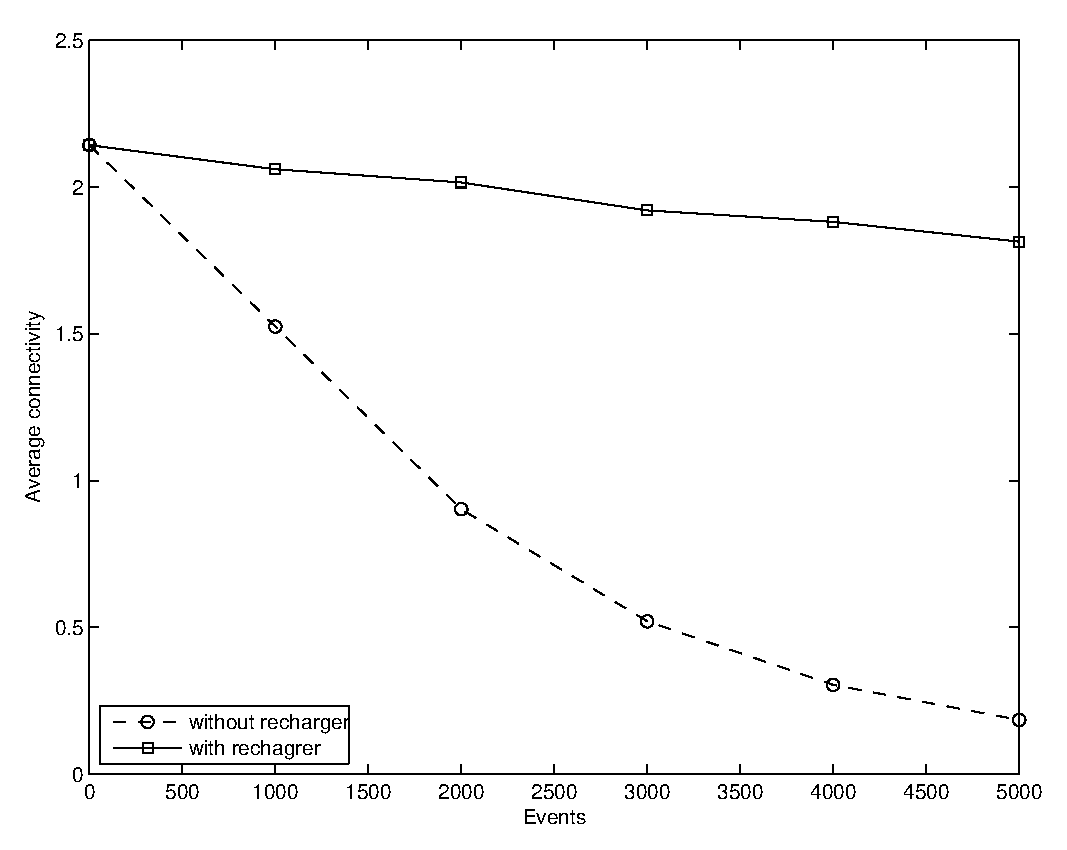
\includegraphics[width=0.32\textwidth]{experiments/classic/1.norechargeVSrecharge/connectivity_leach_nonrc-rc.eps}}
  \subfloat[$E_{i}$]{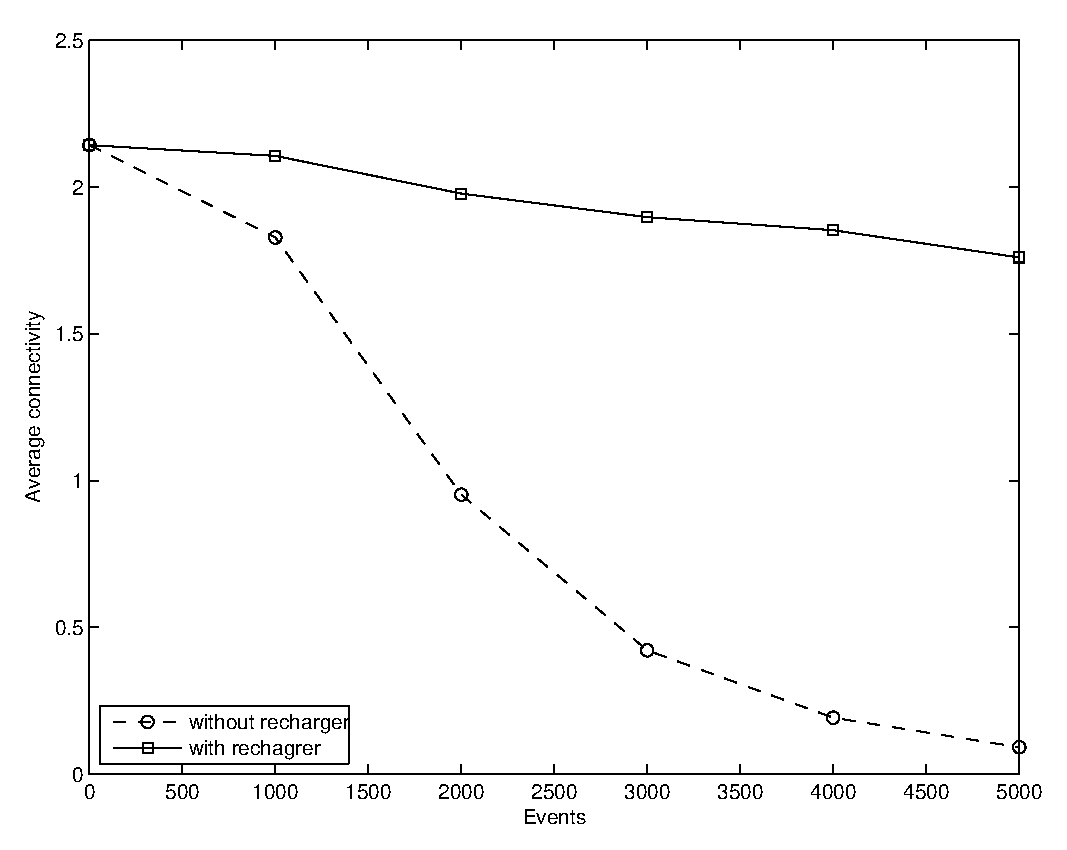
\includegraphics[width=0.32\textwidth]{experiments/classic/1.norechargeVSrecharge/connectivity_ei_nonrc-rc.eps}}
  \caption{Συνδεσιμότητα κατα την πάροδο του χρόνου. Η συνεχόμενη γραμμή αντιστοιχεί στο δίκτυο με κινητό φορτιστή. Υπάρχει σημαντική αύξηση της συνδεσιμότητας του
	δικτύου αν δοθεί μέρος της συνολικής ενέργειας
   στον φορτιστή (εδώ δόθηκε 40\%).}
  \label{fig:1exp_2_1}
\end{figure}


%%%%%%%%%%%%%%%%%%%%%%%%%%%% 3. COVERAGE %%%%%%%%%%%%%%%%%%%%%%%%%%%%%%%%%%%%%

\begin{figure}[H]
  \centering
  \subfloat[Greedy]{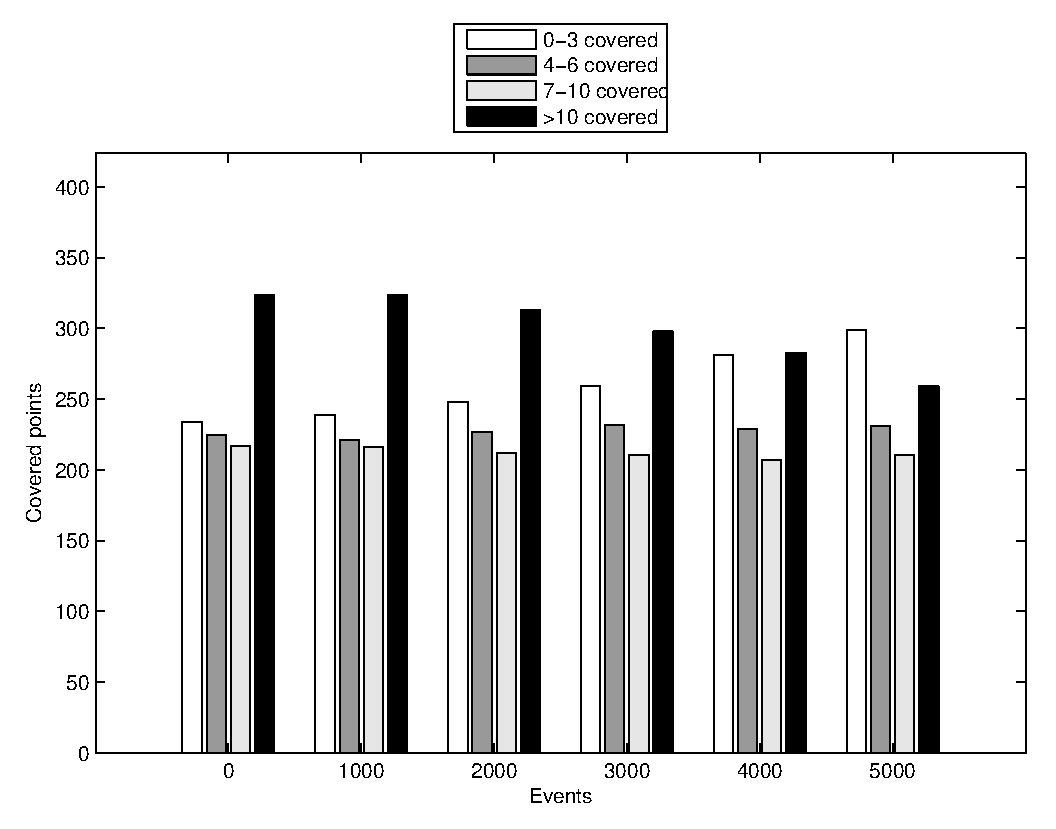
\includegraphics[width=0.48\textwidth]{experiments/classic/1.norechargeVSrecharge/coverage_greedy.eps}}
  \subfloat[Greedy με Φορτιστή]{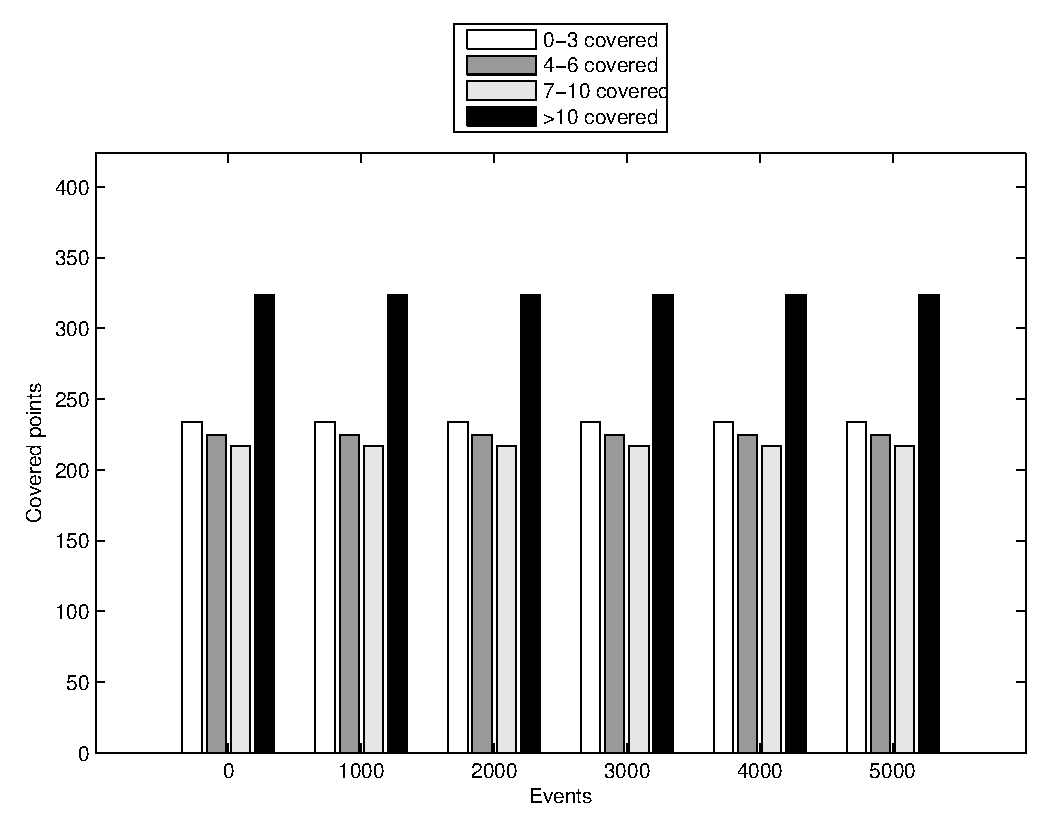
\includegraphics[width=0.48\textwidth]{experiments/classic/1.norechargeVSrecharge/coverage_greedy_rc.eps}}
  \caption{Κάλυψη του δικτύου κατα την πάροδο του χρόνου για το πρωτόκολλο Greedy. Συγκρίνοντας τις 2 γραφικές παραστάσεις φαίνεται οτι στο δίκτυο με φορτιστή
υπάρχει καλύτερη κάλυψη των σημείων του δικτύου.}
  \label{fig:1exp_3_1}
\end{figure}

\begin{figure}[H]
  \centering
  \subfloat[Leach]{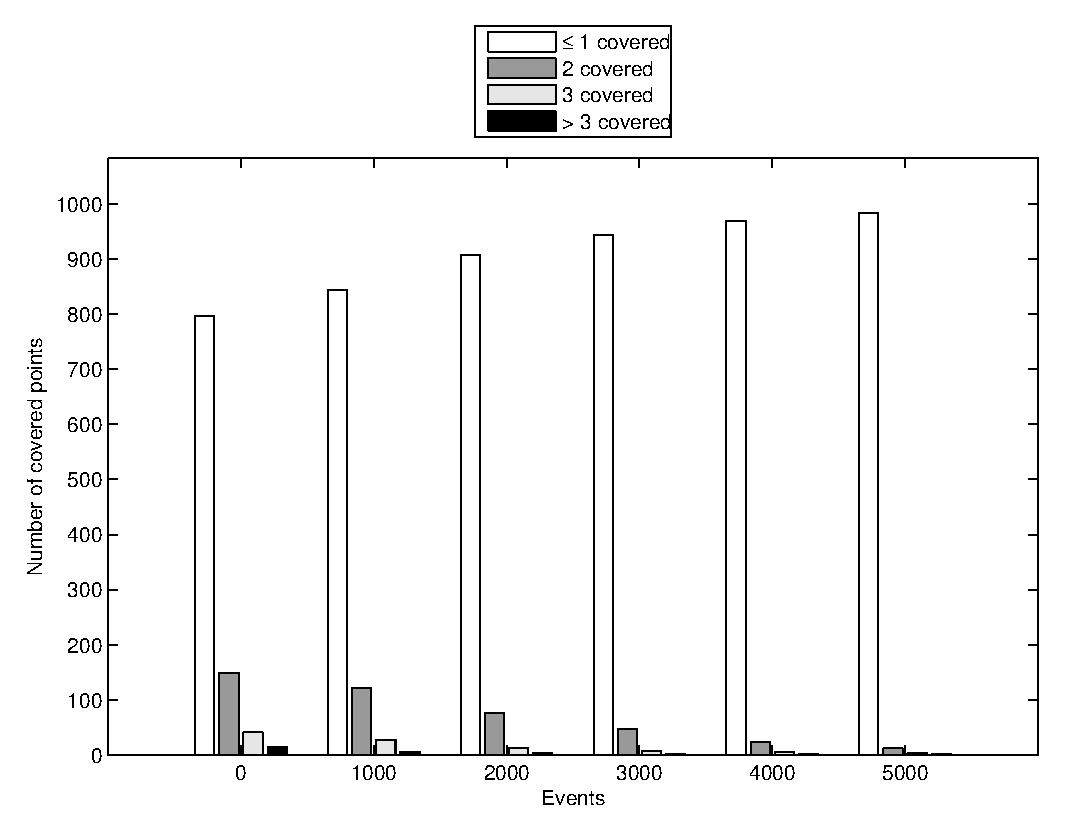
\includegraphics[width=0.48\textwidth]{experiments/classic/1.norechargeVSrecharge/coverage_leach.eps}}
  \subfloat[Leach με Φορτιστή]{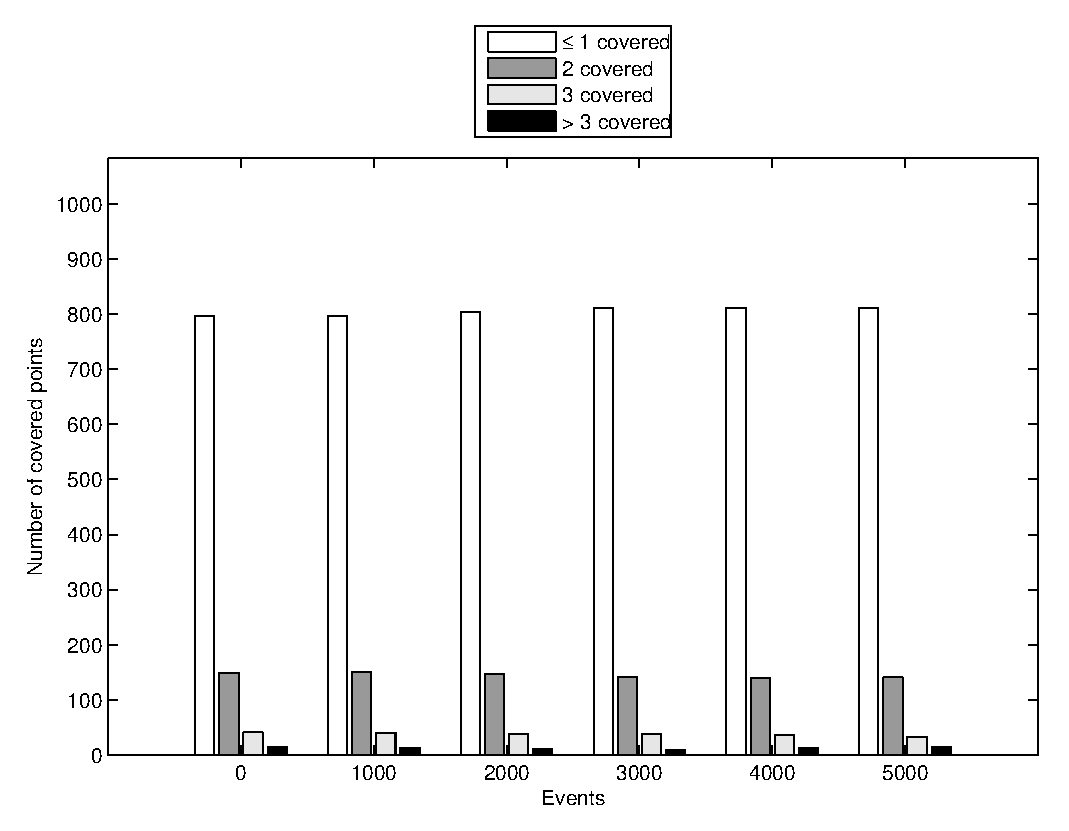
\includegraphics[width=0.48\textwidth]{experiments/classic/1.norechargeVSrecharge/coverage_leach_rc.eps}}
  \caption{Κάλυψη του δικτύου κατα την πάροδο του χρόνου για το πρωτόκολλο Leach. Συγκρίνοντας τις 2 γραφικές παραστάσεις φαίνεται οτι στο δίκτυο με φορτιστή
υπάρχει καλύτερη κάλυψη των σημείων του δικτύου.}
  \label{fig:1exp_3_2}
\end{figure}

\begin{figure}[H]
  \centering
  \subfloat[$\text{E}_{i}$]{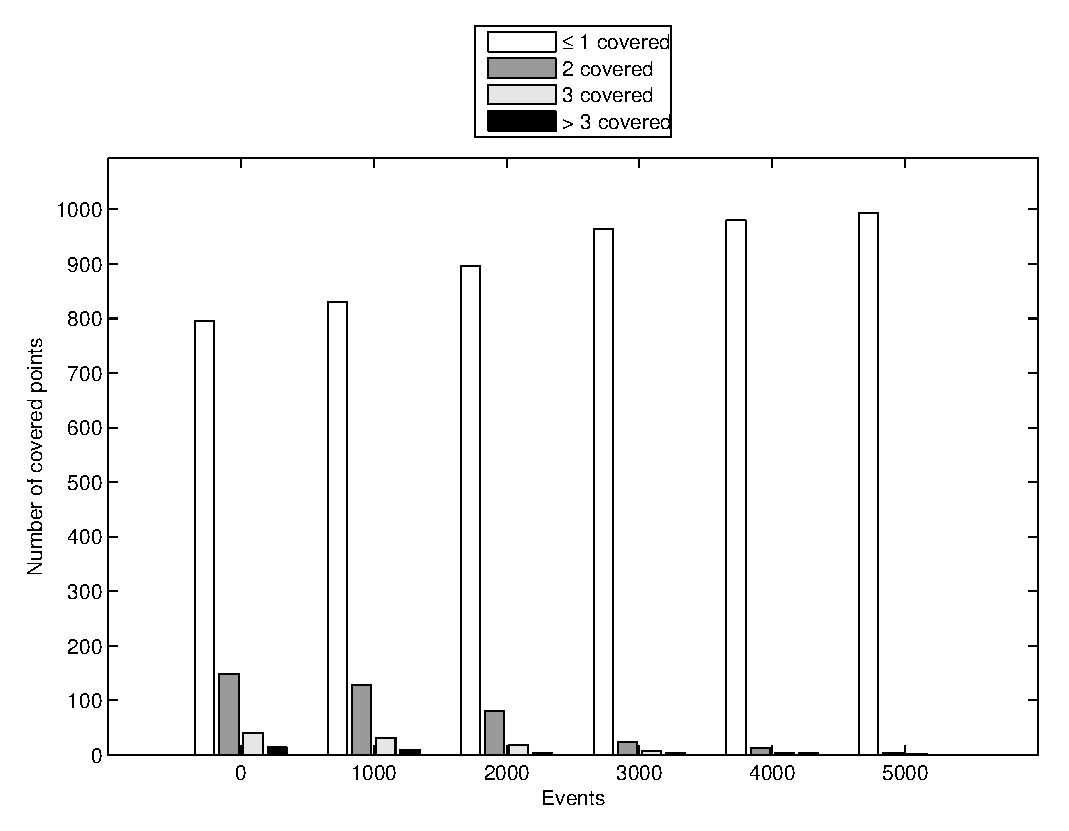
\includegraphics[width=0.48\textwidth]{experiments/classic/1.norechargeVSrecharge/coverage_ei.eps}}
  \subfloat[$\text{E}_{i}$ με Φορτιστή]{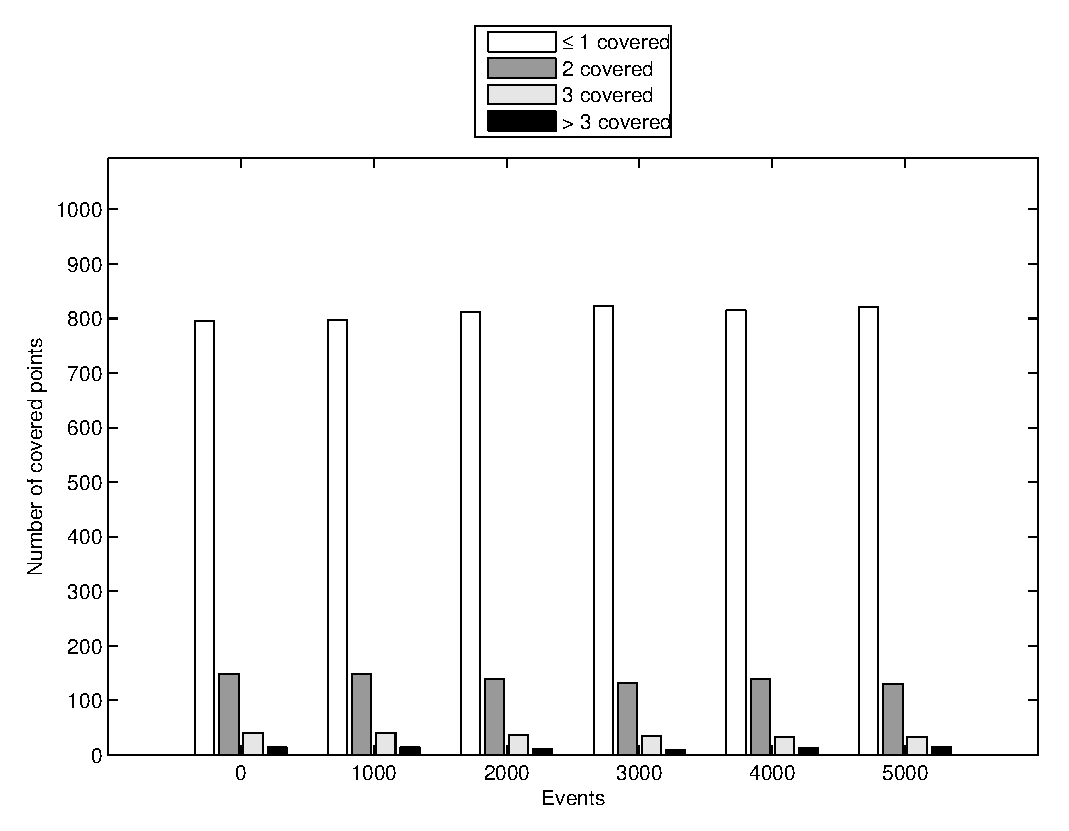
\includegraphics[width=0.48\textwidth]{experiments/classic/1.norechargeVSrecharge/coverage_ei_rc.eps}}
  \caption{Κάλυψη του δικτύου κατα την πάροδο του χρόνου για το πρωτόκολλο $\text{E}_{i}$. Συγκρίνοντας τις 2 γραφικές παραστάσεις φαίνεται οτι στο δίκτυο με φορτιστή
υπάρχει καλύτερη κάλυψη των σημείων του δικτύου.}
  \label{fig:1exp_3_3}
\end{figure}




%%%%%%%%%%%%%%%%%%%%%%%%%%%% 4. ENERGY MAPS %%%%%%%%%%%%%%%%%%%%%%%%%%%%%%%%%%%%%

\begin{figure}[H]
  \centering
  \subfloat[Greedy]{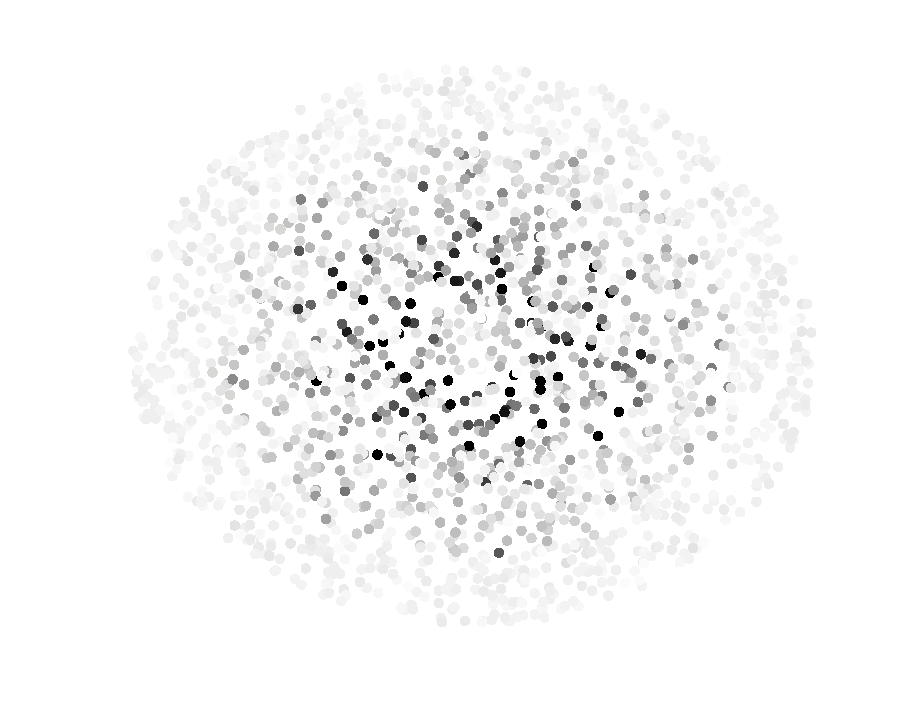
\includegraphics[width=0.48\textwidth]{experiments/classic/1.norechargeVSrecharge/energy_greedy.eps}}
  \subfloat[Greedy με Φορτιστή]{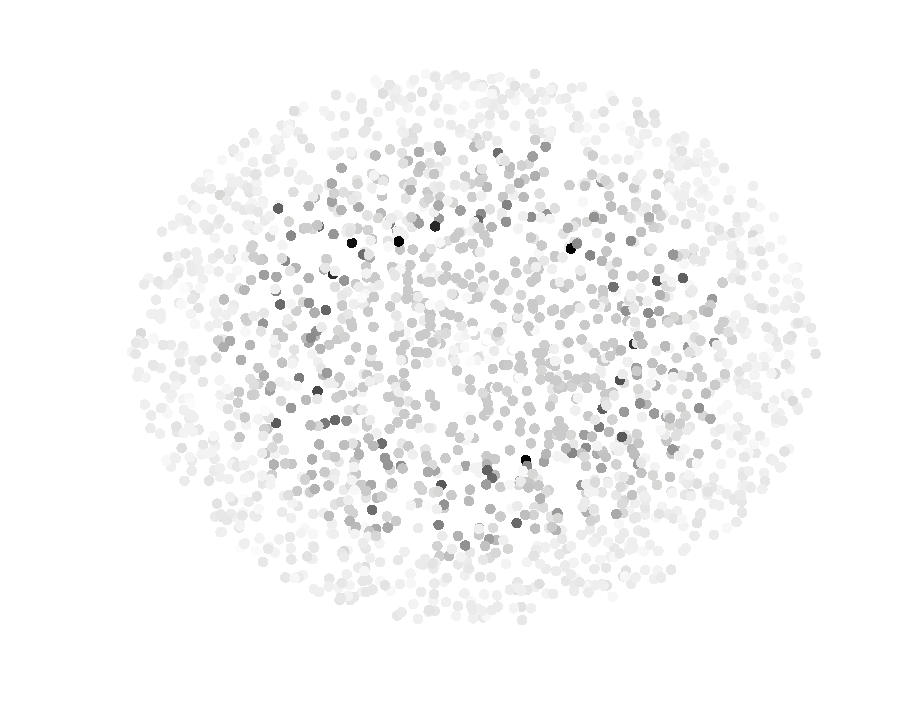
\includegraphics[width=0.48\textwidth]{experiments/classic/1.norechargeVSrecharge/energy_greedy_rc.eps}}
  \caption{Ενεργιακός χάρτης του δικτύου κατα την πάροδο του χρόνου για το πρωτόκολλο Greedy. Όσο πιο μαύρο τόσο λιγότερη ενέργεια έχει ο κόμβος. Συγκρίνοντας τις 2
γραφικές παραστάσεις φαίνεται οτι στο δίκτυο με φορτιστή υπάρχει καλύτερη εξισορρόπηση ενέργειας.}
  \label{fig:1exp_4_1}
\end{figure}

\begin{figure}[H]
  \centering
  \subfloat[Leach]{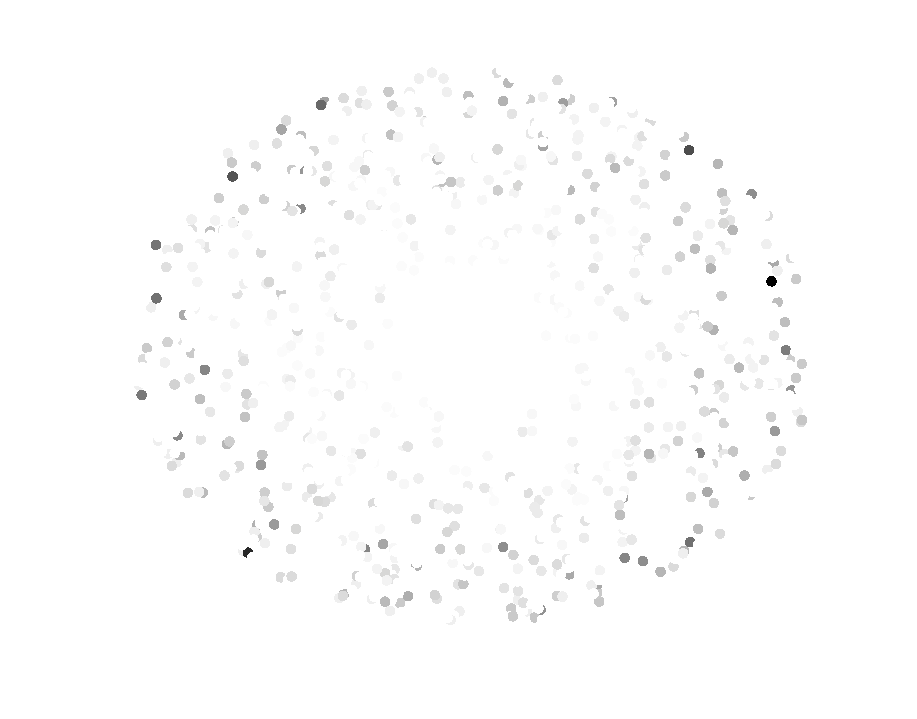
\includegraphics[width=0.48\textwidth]{experiments/classic/1.norechargeVSrecharge/energy_leach.eps}}
  \subfloat[Leach με Φορτιστή]{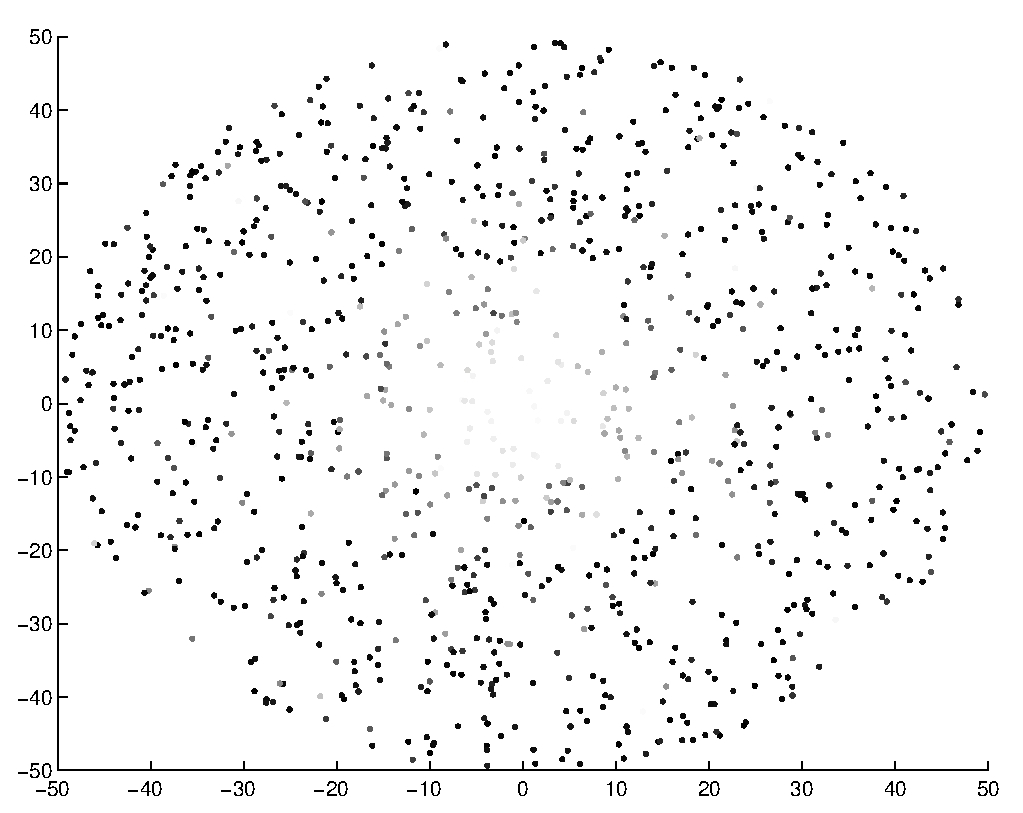
\includegraphics[width=0.48\textwidth]{experiments/classic/1.norechargeVSrecharge/energy_leach_rc.eps}}
  \caption{Κάλυψη του δικτύου κατα την πάροδο του χρόνου για το πρωτόκολλο Leach. Όσο πιο μαύρο τόσο λιγότερη ενέργεια έχει ο κόμβος. Συγκρίνοντας τις 2 γραφικές
παραστάσεις φαίνεται οτι στο δίκτυο με φορτιστή υπάρχει καλύτερη εξισορρόπηση ενέργειας.}
  \label{fig:1exp_4_2}
\end{figure}

\begin{figure}[H]
  \centering
  \subfloat[$\text{E}_{i}$]{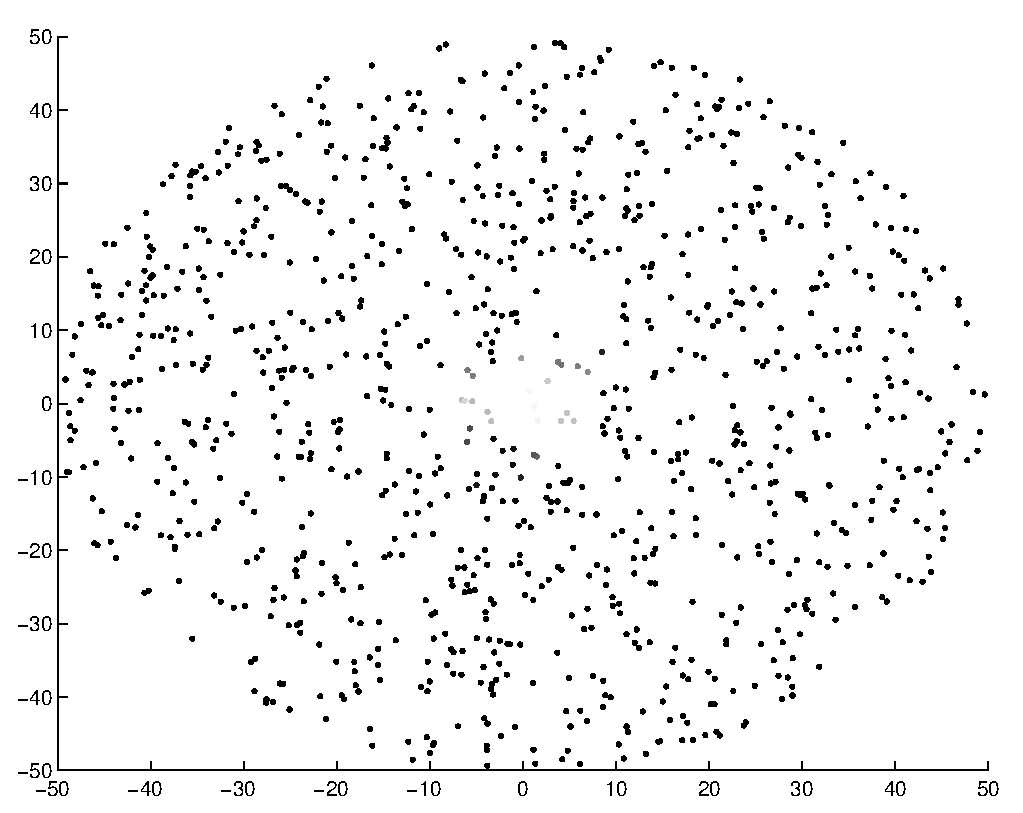
\includegraphics[width=0.48\textwidth]{experiments/classic/1.norechargeVSrecharge/energy_ei.eps}}
  \subfloat[$\text{E}_{i}$ με Φορτιστή]{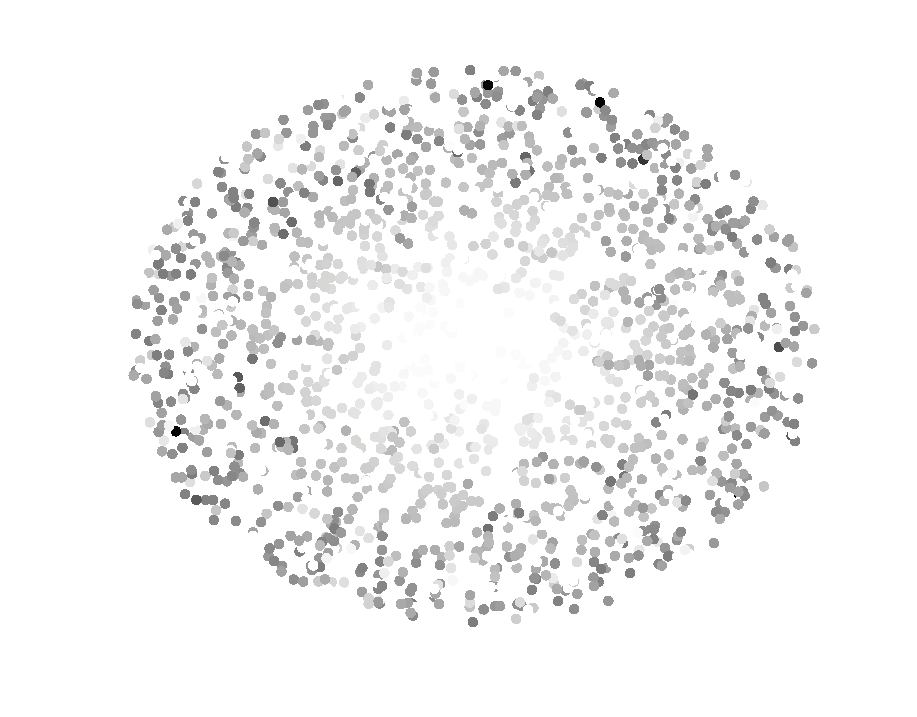
\includegraphics[width=0.48\textwidth]{experiments/classic/1.norechargeVSrecharge/energy_ei_rc.eps}}
  \caption{Κάλυψη του δικτύου κατα την πάροδο του χρόνου για το πρωτόκολλο $\text{E}_{i}$. Όσο πιο μαύρο τόσο λιγότερη ενέργεια έχει ο κόμβος. Συγκρίνοντας τις 2
γραφικές παραστάσεις φαίνεται οτι στο δίκτυο με φορτιστή υπάρχει καλύτερη εξισορρόπηση ενέργειας.}
  \label{fig:1exp_4_3}
\end{figure}

Όπως φαίνεται και από τα σχεδιαγράμματα, στην περίπτωση που στο δίκτυο χρησιμοποιείται φόρτιση, αυτό έχει μεγαλύτερο χρόνο ζωής αφού ο φορτιστής επιλέγει να δώσει
την ενέργεια εκεί που πραγματικά την χρειάζεται.







\section{Ολική και Μερική Φόρτιση}\label{sc:result2}
Η πρώτη παραμετροποίηση ή στρατηγική της διαδικασίας της φόρτισης που μελετάται είναι μέχρι ποιο επίπεδο θα πρέπει ο κινητός φορτιστής να φορτίζει τους στατικούς
κόμβους. Οι 2 στρατηγικές που συγκρίνονται είναι:
\begin{itemize}
  \item \textbf{Oλική φόρτιση}, δηλαδή σε κάθε καινούργια φόρτιση ο φορτιστής φορτίζει μέχρις ότου ο στατικός κόμβος να ανακτήσει πλήρως την αρχική του ενέργεια
  \item \textbf{Μερική φόρτιση}, δηλαδή σε κάθε καινούργια φόρτιση ο φορτίζει μέχρις ότου για την ενέργεια του στατικού κόμβου $e_{i}$ ισχύει οτι
\begin{align*}
e_{i} \approx \frac{E^{curr}_{MC}}{E^{init}_{MC}}\cdot E^{max}_{sensor}
\end{align*}
όπου $E^{curr}_{MC}$, $E^{init}_{MC}$ η τρέχουσα ενέργεια και αρχική ενέργεια του κινητού φορτιστή ενώ $E^{max}_{sensor}$ η αρχική ενέργεια ενός στατικού κόμβου.
\end{itemize}
Ξανά οι στατικοί κόμβοι σε αυτή την περίπτωση δεν ξεκινάνε με πλήρη αρχική ενέργεια αλλά με ένα ποσοστό της αρχικής ενέργειας, και συγκεκριμένα
με το 60\% της αρχικής τους ενέργειας και επομένως ο φορτιστής κατέχει αρχικά το 40\% της αρχικής ολικής ενέργειας του δικτύου. Τα αποστελέσματα των πειραμάτων
φαίνονται στις εικόνες \ref{fig:2exp_1_1}, \ref{fig:2exp_2_1}, \ref{fig:2exp_3_1}, \ref{fig:2exp_3_2} και \ref{fig:2exp_3_3}. Η στρατηγική της μερικής φόρτισης
κερδίζει την στρατηγική της ολικής φόρτισης στα πρωτόκολλα Leach και $\text{E}_{i}$ ενώ χάνει για πολύ λίγο στο πρωτόκολλο Greedy. Αυτό συμβάινει επειδή στο
πρωτόκολλο Greedy, υπάρχει ένας μικρός αριθμός κόμβων, αυτοί που είναι κοντά στην πηγή, οι οποίοι έχουν πολύ μεγάλο ρυθμό κατανάλωσης ενέργειας. Επομένως
φορτίζοντάς τους πλήρως είναι πιο πιθανόν να μείνουν ζωντανοί μέχρι να ξαναέρθει σε αυτούς ο φορτιστής. Αντίθετα στα 2 άλλα πρωτόκολλα, τα οποία παράγουν ένα πιο
εξισορροπημένο, ενεργειακά, δίκτυο η στρατηγική της πλήρης φόρτιση ξοδεύει πολύ πιο γρήγορα την πολύτιμη ενέργεια του φορτιστή και ενώ κερδίζει αρχικά, μόλις
τελειώσει η ενέργεια του φορτιστή, το οποίο συμβαίνει γρήγορα, οι κόμβοι του δικτύου αρχίζουν και πεθαίνουν.


%%%%%%%%%%%%%%%%%%%%%%%%%%%% 1. LIFETIME %%%%%%%%%%%%%%%%%%%%%%%%%%%%%%%%%%%%%
\begin{figure}[H]
  \centering
  \subfloat[Greedy]{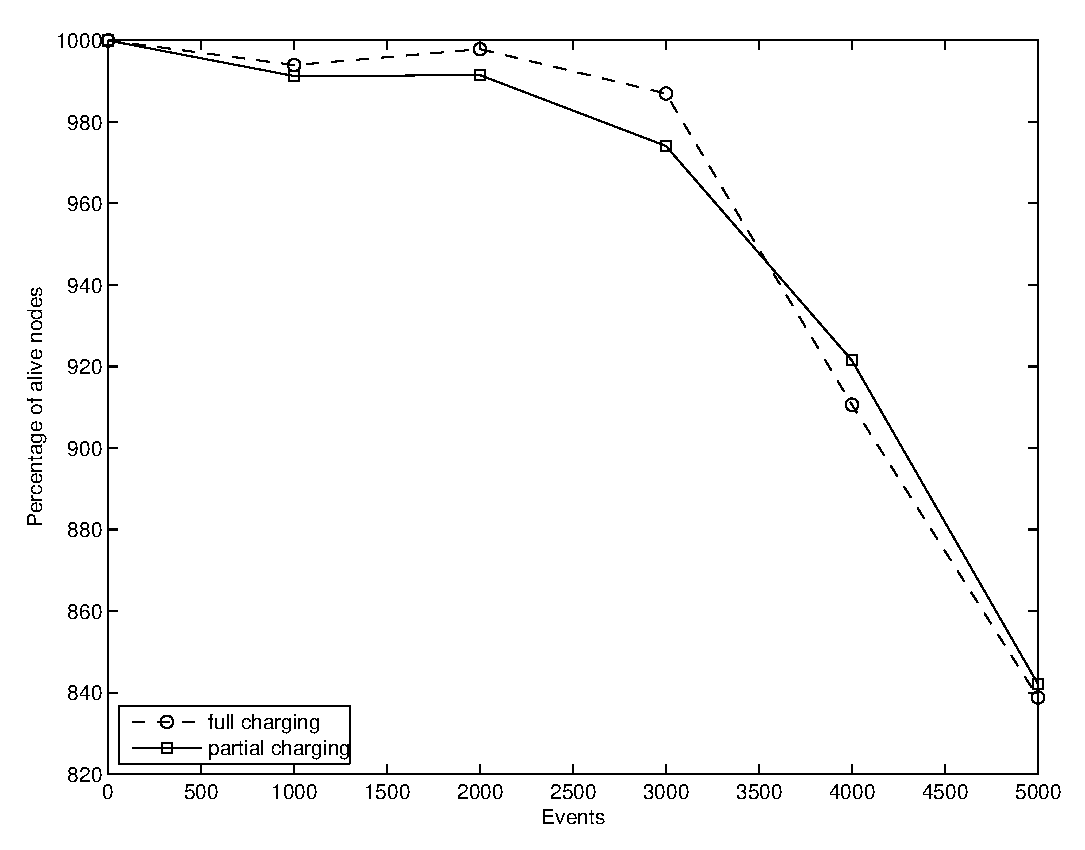
\includegraphics[width=0.32\textwidth]{experiments/classic/2.partialVSfull/alive_nodes_greedy_rc_full-per.eps}}
  \subfloat[Leach]{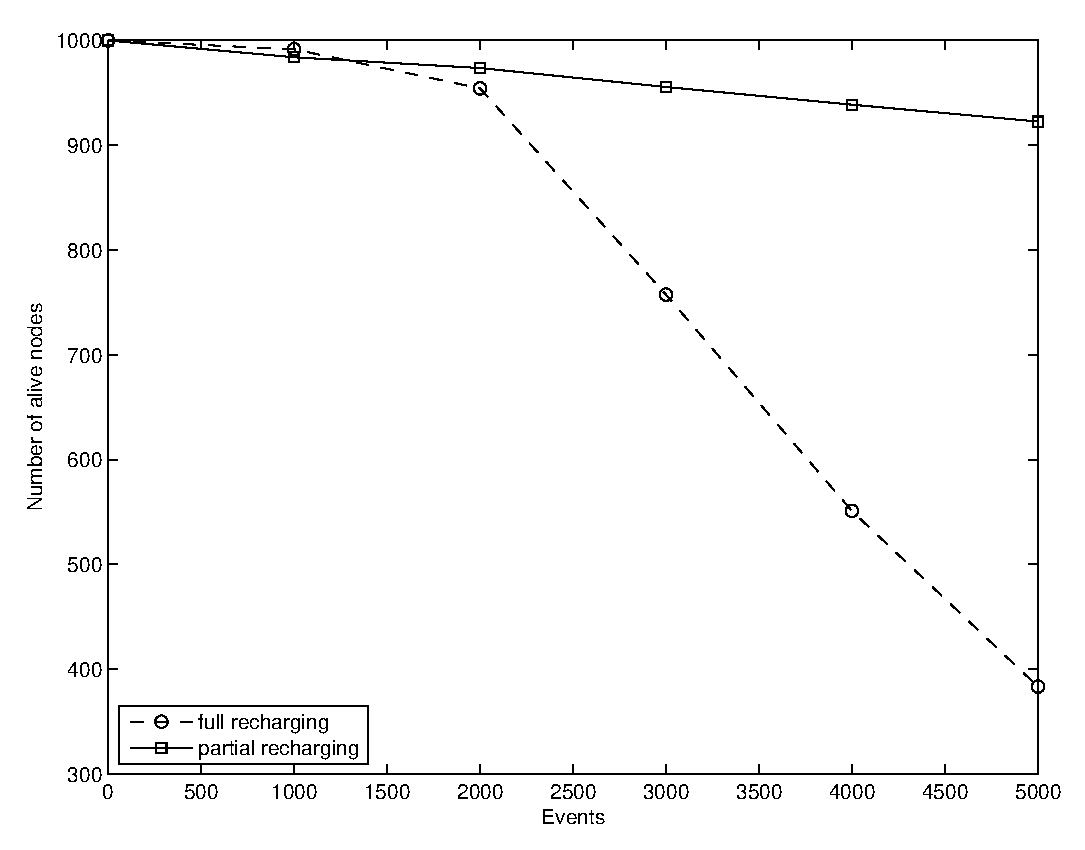
\includegraphics[width=0.32\textwidth]{experiments/classic/2.partialVSfull/alive_nodes_leach_rc_full-per.eps}}
  \subfloat[$\text{E}_{i}$]{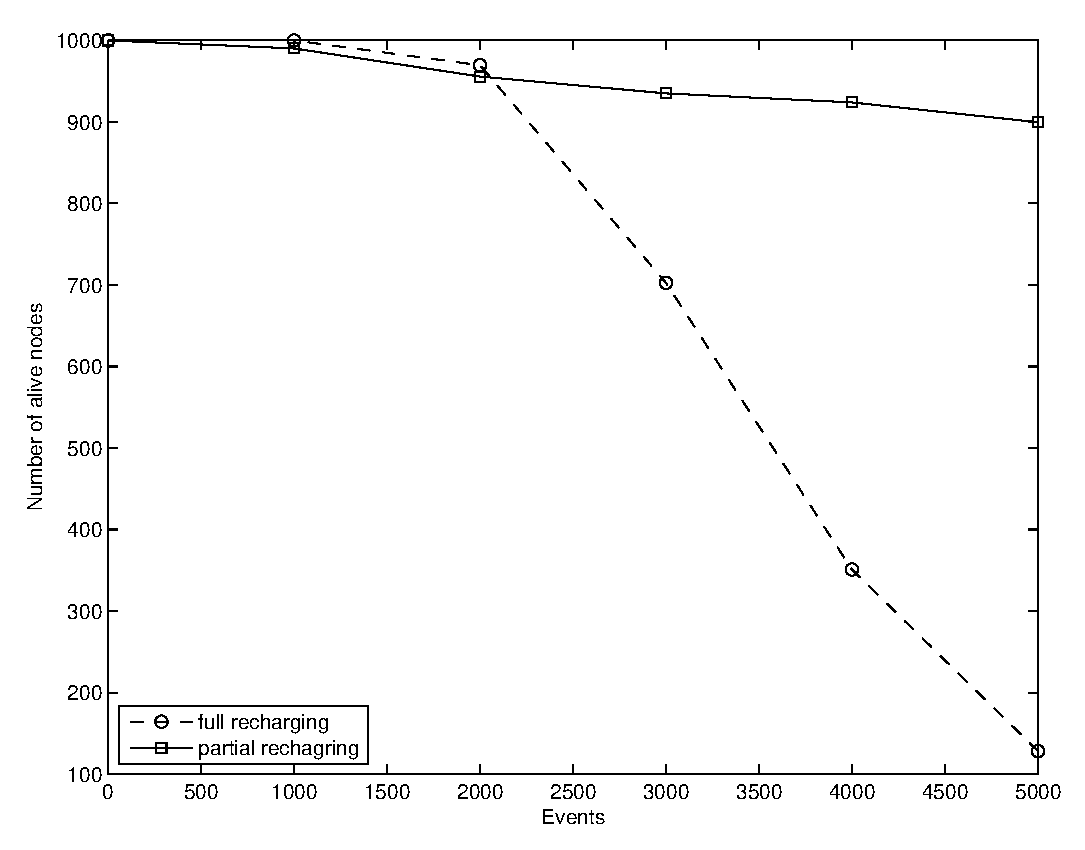
\includegraphics[width=0.32\textwidth]{experiments/classic/2.partialVSfull/alive_nodes_ei_rc_full-per.eps}}
  \caption{Ζωντανοί κόμβοι κατά την πάροδο του χρόνου. Η συνεχόμενη γραμμή αντιστοιχεί στην μερική φόρτιση. Στο Greedy πρωτόκολλο, η πλήρης φόρτιση έχει
ελάχιστα καλύτερα αποτελέσματα. Αυτό συμβαίνει γιατί ο ρυθμός κατανάλωσης των κόμβων που είναι κοντά στην Πηγή είναι πολύ μεγάλος και επομένως συμφέρει να φορτίζονται
πλήρως. Αντίθετα στα άλλα 2 πρωτόκολλα, η μερική φόρτιση
υπερνικάει την στρατηγική της πλήρους φόρτισης.}
  \label{fig:2exp_1_1}
\end{figure}

%%%%%%%%%%%%%%%%%%%%%%%%%%%% 2. CONNECTIVITY %%%%%%%%%%%%%%%%%%%%%%%%%%%%%%%%%%%%%
\begin{figure}[H]
  \centering
  \subfloat[Greedy]{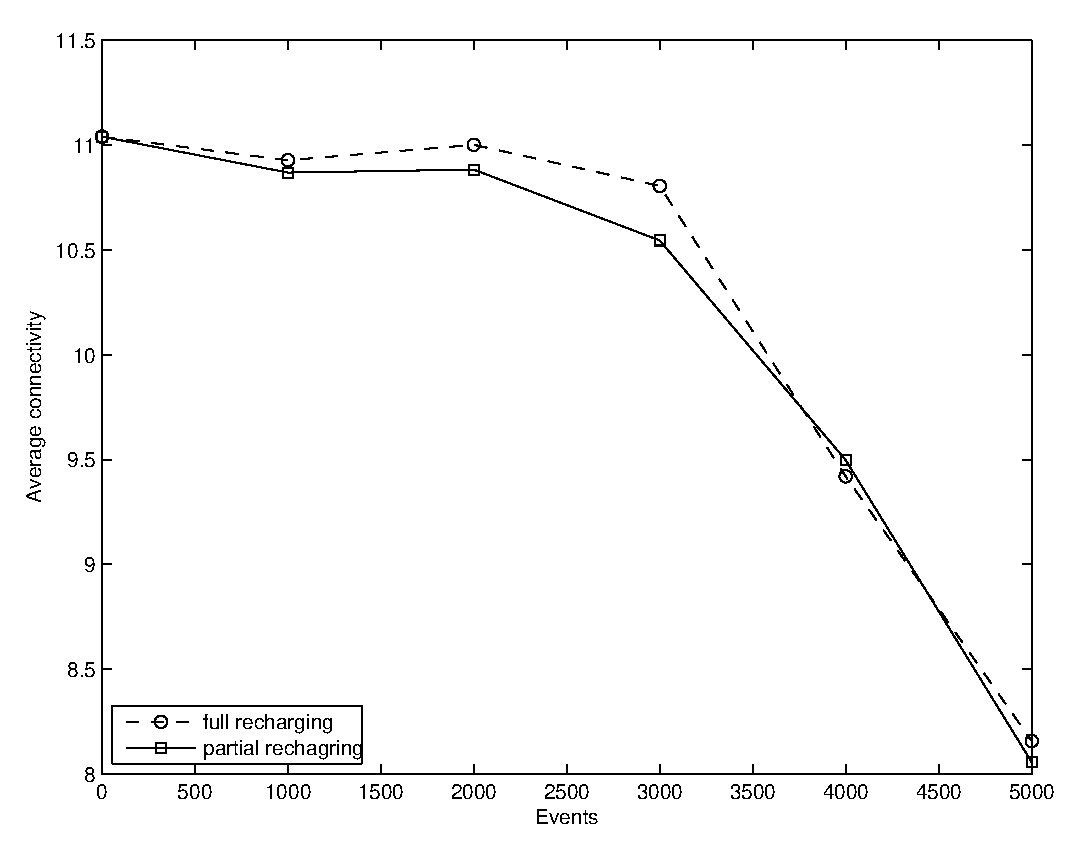
\includegraphics[width=0.32\textwidth]{experiments/classic/2.partialVSfull/connectivity_greedy_rc_full-per.eps}}
  \subfloat[Leach]{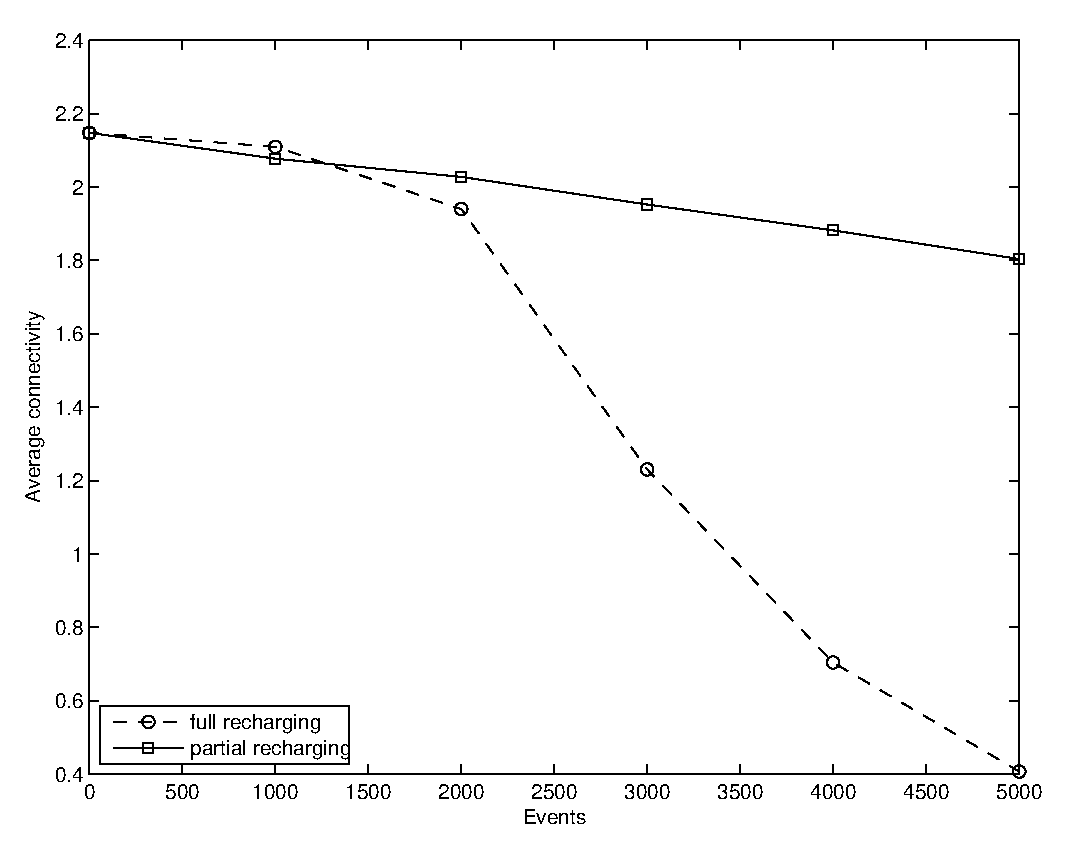
\includegraphics[width=0.32\textwidth]{experiments/classic/2.partialVSfull/connectivity_leach_rc_full-per.eps}}
  \subfloat[$\text{E}_{i}$]{\includegraphics[width=0.32\textwidth]{experiments/classic/2.partialVSfull/connectivity_ei_rc_full-per.eps}}
  \caption{Συνδεσιμότητα κατα την πάροδο του χρόνου. Η συνεχόμενη γραμμή αντιστοιχεί στην μερική φόρτιση. Στο Greedy πρωτόκολλο, η πλήρης φόρτιση έχει ελάχιστα
καλύτερα αποτελέσματα. Αυτό συμβαίνει γιατί ο ρυθμός κατανάλωσης των κόμβων που είναι κοντά στην Πηγή είναι πολύ μεγάλος και επομένως με την μερική φόρτιση οι κόμβοι
πεθαίνουν πιο γρήγορα και το δίκτυο αποσυνδέεται. Αντίθετα στα άλλα 2 πρωτόκολλα, η μερική φόρτιση υπερνικάει την στρατηγική της πλήρους φόρτισης.}
  \label{fig:2exp_2_1}
\end{figure}


%%%%%%%%%%%%%%%%%%%%%%%%%%%% 3. COVERAGE %%%%%%%%%%%%%%%%%%%%%%%%%%%%%%%%%%%%%
\begin{figure}[H]
  \centering
  \subfloat[Greedy με ολική Φόρτιση]{\includegraphics[width=0.48\textwidth]{experiments/classic/2.partialVSfull/coverage_greedy_rc_full.eps}}
  \subfloat[Greedy με μερική Φόρτιση]{\includegraphics[width=0.48\textwidth]{experiments/classic/2.partialVSfull/coverage_greedy_rc_per.eps}}
  \caption{Κάλυψη του δικτύου κατα την πάροδο του χρόνου για το πρωτόκολλο Greedy. Οι δύο στρατηγικές έχουν παρόμοια αποτελέσματα. Αυτό
συμβαίνει γιατί ο ρυθμός κατανάλωσης των κόμβων που είναι κοντά στην Πηγή είναι πολύ μεγάλος και επομένως η στρατηγική της μερικής φόρτισης δεν αποδίδει καλά.}
  \label{fig:2exp_3_1}
\end{figure}

\begin{figure}[H]
  \centering
  \subfloat[Leach με ολική Φόρτιση]{\includegraphics[width=0.48\textwidth]{experiments/classic/2.partialVSfull/coverage_leach_rc_full.eps}}
  \subfloat[Leach με μερική Φόρτιση]{\includegraphics[width=0.48\textwidth]{experiments/classic/2.partialVSfull/coverage_leach_rc_per.eps}}
  \caption{Κάλυψη του δικτύου κατα την πάροδο του χρόνου για το πρωτόκολλο Leach. Είναι εμφανές οτι η στρατηγική της μερικής φόρτισης έχει καλύτερα αποτελέσματα.}
  \label{fig:2exp_3_2}
\end{figure}

\begin{figure}[H]
  \centering
  \subfloat[$\text{E}_{i}$ με ολική Φόρτιση]{\includegraphics[width=0.48\textwidth]{experiments/classic/2.partialVSfull/coverage_ei_rc_full.eps}}
  \subfloat[$\text{E}_{i}$ με μερική Φόρτιση]{\includegraphics[width=0.48\textwidth]{experiments/classic/2.partialVSfull/coverage_ei_rc_per.eps}}
  \caption{Κάλυψη του δικτύου κατα την πάροδο του χρόνου για το πρωτόκολλο $\text{E}_{i}$. Είναι εμφανές οτι η στρατηγική της μερικής φόρτισης έχει καλύτερα
αποτελέσματα.}
  \label{fig:2exp_3_3}
\end{figure}


\section{Ποσοστό Ενέργειας στον Φορτιστή}\label{sc:result3}
H επόμενη παραμετροποίηση που εξερευνάται είναι η βέλτιστη κατανομή ενέργειας ανάμεσα στον κινητό φορτιστή και τους στατικούς κόμβους σε σχέση με την συνολική αρχική
ενέργεια που διατίθεται στο δίκτυο. Διεξάχθηκαν πειράματα με διάφορες κατανομές ενέργειας και πιο συγκεκριμένα με το 20\%, 40\%, 60\%, και 80\% της συνολικής αρχικής
ενέργειας να δίνεται στον κινητό φορτιστή και το υπόλοιπο στους στατικούς κόμβους. Χρησιμοποιήθηκε ο προσαρμοστικός φορτιστής. Η πειραματική αξιολόγηση έδειξε οτι ένα
ποσοστό κοντά στο 20\% είναι η πιο αποδοτική στρατηγική. Τα αποτελέσματα των πειραμάτων φαίνονται στις εικόνες \ref{fig:3exp_1_1}, \ref{fig:3exp_1_2} και
\ref{fig:3exp_1_3}. Στο Greedy πρωτόκολλο \ref{fig:3exp_1_1}, καθώς ένα μικρό μέρος του δικτύου έχει πολύ μεγάλη κατανάλωση ενέργεια, μια στρατηγική που θα δίνει στον
φορτιστή το 60\% της συνολικής αρχικής ενέργειας του δικτύου φαίνεται να είναι η πιο αποδοτική. Επίσης φαίνεται στην περίπτωση που δοθεί 80\% στον φορτιστή, στην αρχή
πεθαίνουν πολλοί κόμβοι (καθώς έχουν μόνο το 20\% της ενέργειάς τους) αλλά μετά από λίγο ο φορτιστής μπορεί και το επαναφέρει, κυρίως λόγω της φύσης του πρωτοκόλλου
(λίγοι κόμβοι με μεγάλο ρυθμό κατανάλωσης ενέργειας). Αντίθετα στα πρωτόκολλα Leach \ref{fig:3exp_1_2} και $\text{E}_{i}$ \ref{fig:3exp_1_3} μια στρατηγική που δίνει
το 20\%-30\% της αρχικής ενέργειας στον φορτιστή φαίνεται να είναι η βέλτιστη. Επίσης φαίνεται οτι όταν ο φορτιστής έχει το 80\% της ενέργειας επειδή τα πρωτόκολλα
έχουν καλύτερη εξισορρόπηση ενέργειας, ο φορτιστής δεν μπορεί να επαναφέρει το δίκτυο καθώς οι κόμβοι πεθαίνουν πιο κοντά ο ένας στον άλλον από ότι στο Greedy
πρωτόκολλο.



%%%%%%%%%%%%%%%%%%%%%%%%%%%% 1. LIFETIME %%%%%%%%%%%%%%%%%%%%%%%%%%%%%%%%%%%%%
\begin{figure}[H]
  \centering
  \includegraphics[width=0.9\textwidth]{experiments/classic/3.smallVSbigpercentage/alive_nodes_greedy_rc_per_our.eps}
  \caption{Ζωντανοί κόμβοι κατά την πάροδο του χρόνου στο Greedy πρωτόκολλο με ποικίλα ποσοστά ενέργειας στον κινητό φορτιστή. Μία ποσότητα κοντά στο 60\% στον
φορτιστή φαίνεται να είναι η βέλτιστη, κυρίως λόγω της φύσης του πρωτοκόλλου.}
  \label{fig:3exp_1_1}
\end{figure}

\begin{figure}[H]
  \centering
   \includegraphics[width=0.9\textwidth]{experiments/classic/3.smallVSbigpercentage/alive_nodes_leach_rc_per_our.eps}
  \caption{Ζωντανοί κόμβοι κατά την πάροδο του χρόνου στο Leach πρωτόκολλο με ποικίλα ποσοστά ενέργειας στον κινητό φορτιστή. Μία ποσότητα κοντά στο 30\% στον
φορτιστή φαίνεται να είναι η βέλτιστη.}
  \label{fig:3exp_1_2}
\end{figure}

\begin{figure}[H]
  \centering
   \includegraphics[width=0.9\textwidth]{experiments/classic/3.smallVSbigpercentage/alive_nodes_ei_rc_per_our.eps}
  \caption{Ζωντανοί κόμβοι κατά την πάροδο του χρόνου στο $\text{E}_{i}$ πρωτόκολλο με ποικίλα ποσοστά ενέργειας στον κινητό φορτιστή. Μία ποσότητα κοντά στο 30\%
στον φορτιστή φαίνεται να είναι η βέλτιστη.}
  \label{fig:3exp_1_3}
\end{figure}


\section{Σύγκριση Διαδρομών Φορτιστή}\label{sc:result4}
Αφού έχουν βρεθεί οι βέλτιστες στρατηγικές για τον κινητό φορτιστή (μερική φόρτιση, 20\% της αρχικής ενέργειας), σε αυτήν την ενότητα συγκρίνεται ο προσαρμοστικός
φορτιστής με τον αλγόριθμο καθολικής γνώσης καθώς και με τους υπόλοιπους αφελής αλγορίθμους. Στην πίνακα \ref{tab:dist} φαίνονται οι διαδρομές που καλύπτει ο κάθε
φορτιστής. Όπως φαίνεται ο προσαρμοστικός φορτιστής είναι πολύ κοντά στον φορτιστή καθολικής γνώσεις όσον αφορά την απόσταση που διανύει. Τα αποτελέσματα των
πειραμάτων φαίνονται στις εικόνες \ref{fig:4exp_1_1}, \ref{fig:4exp_1_2}, \ref{fig:4exp_1_3}, \ref{fig:4exp_2_1}, \ref{fig:4exp_2_2} και \ref{fig:4exp_2_3}. Από τα
αποτελέσματα διακρίνεται οτι ο προσαρμοστικός φορτιστής, ενώ χρησιμοποιεί μόνο τοπική πληροφορία, τα πάει αρκετά καλά ειδικά στις περιπτώσεις των πρωτοκόλλων Leach
και $\text{E}_{i}$.

\begin{table}[H]
%\begin{center}
\begin{tabular}{r|c|c|c|}
& Greedy & E$_i$ & LEACH\\\cline{2-4}\cline{2-4}
global knowledge & 48974 & 64330 & 57458\\\cline{2-4}
spiral & 64167 & 64167 & 64167\\\cline{2-4}
random walk & 181135 & 222462 & 222447 \\\cline{2-4}
diameter & 152252 & 172734 & 173169\\\cline{2-4}
adaptive charger & 42412 & 37856 & 38641\\\cline{2-4}
\end{tabular}
%\end{center}
\caption{Distance travelled by chargers}
\label{tab:dist}
\end{table}

%%%%%%%%%%%%%%%%%%%%%%%%%%%% 1. LIFETIME %%%%%%%%%%%%%%%%%%%%%%%%%%%%%%%%%%%%%
\begin{figure}[H]
  \centering
  \includegraphics[width=0.9\textwidth]{experiments/classic/4.ourVSnaive/alive_nodes_greedy_rc_per_our-spiral-random-diameter-heuristic.eps}
  \caption{Ζωντανοί κόμβοι κατά την πάροδο του χρόνου στο Greedy πρωτόκολλο για τις διάφορες διαδρομές του κινητού φορτιστή. Χρησιμοποιείται μερική φόρτιση και έχει
δωθεί το 20\% της ενέργειας στον φορτιστή.}
  \label{fig:4exp_1_1}
\end{figure}

\begin{figure}[H]
  \centering
  \includegraphics[width=0.9\textwidth]{experiments/classic/4.ourVSnaive/alive_nodes_leach_rc_per_our-spiral-random-diameter-heuristic.eps}
  \caption{Ζωντανοί κόμβοι κατά την πάροδο του χρόνου στο Leach πρωτόκολλο για τις διάφορες διαδρομές του κινητού φορτιστή. Χρησιμοποιείται μερική φόρτιση και έχει
δωθεί το 20\% της ενέργειας στον φορτιστή.}
  \label{fig:4exp_1_2}
\end{figure}

\begin{figure}[H]
  \centering
  \includegraphics[width=0.9\textwidth]{experiments/classic/4.ourVSnaive/alive_nodes_ei_rc_per_our-spiral-random-diameter-heuristic.eps}
  \caption{Ζωντανοί κόμβοι κατά την πάροδο του χρόνου στο $\text{E}_{i}$ πρωτόκολλο για τις διάφορες διαδρομές του κινητού φορτιστή. Χρησιμοποιείται μερική φόρτιση
και έχει δωθεί το 20\% της ενέργειας στον φορτιστή.}
  \label{fig:4exp_1_3}
\end{figure}



%%%%%%%%%%%%%%%%%%%%%%%%%%%% 2. COVERAGE %%%%%%%%%%%%%%%%%%%%%%%%%%%%%%%%%%%%%
\begin{figure}[H]
  \centering
  \subfloat[Προσαρμοστικός Φορτιστής]{\includegraphics[width=0.48\textwidth]{experiments/classic/4.ourVSnaive/coverage_greedy_rc_per_our.eps}}
  \subfloat[Καθολικής Γνώσης Φορτιστής]{\includegraphics[width=0.48\textwidth]{experiments/classic/4.ourVSnaive/coverage_greedy_rc_per_heuristic.eps}}
  \caption{Κάλυψη του δικτύου κατα την πάροδο του χρόνου για το πρωτόκολλο Greedy. Χρησιμοποιείται μερική φόρτιση και έχει δωθεί το 20\% της ενέργειας στον φορτιστή.}
  \label{fig:4exp_2_1}
\end{figure}

\begin{figure}[H]
  \centering
  \subfloat[Προσαρμοστικός Φορτιστής]{\includegraphics[width=0.48\textwidth]{experiments/classic/4.ourVSnaive/coverage_leach_rc_per_our.eps}}
  \subfloat[Καθολικής Γνώσης Φορτιστής]{\includegraphics[width=0.48\textwidth]{experiments/classic/4.ourVSnaive/coverage_leach_rc_per_heuristic.eps}}
  \caption{Κάλυψη του δικτύου κατα την πάροδο του χρόνου για το πρωτόκολλο Leach. Χρησιμοποιείται μερική φόρτιση και έχει δωθεί το 20\% της ενέργειας στον φορτιστή.}
  \label{fig:4exp_2_2}
\end{figure}

\begin{figure}[H]
  \centering
  \subfloat[Προσαρμοστικός Φορτιστής]{\includegraphics[width=0.48\textwidth]{experiments/classic/4.ourVSnaive/coverage_ei_rc_per_our.eps}}
  \subfloat[Καθολικής Γνώσης Φορτιστής]{\includegraphics[width=0.48\textwidth]{experiments/classic/4.ourVSnaive/coverage_ei_rc_per_heuristic.eps}}
  \caption{Κάλυψη του δικτύου κατα την πάροδο του χρόνου για το πρωτόκολλο $\text{E}_{i}$. Χρησιμοποιείται μερική φόρτιση και έχει
δωθεί το 20\% της ενέργειας στον φορτιστή.}
  \label{fig:4exp_2_3}
\end{figure}























\section{Αυξάνοντας τον αριθμό των κόμβων}\label{sc:result5}
Σε αυτό το πείραμα, ο αριθμός των κόμβων αυξάνεται δραματικά. Συγκεκριμένα από 1000 κόμβους που ήταν στα προηγούμενα πειράματα, ο αριθμός των κόμβων γίνεται 4000. Ο
κινητός φορτιστής πλέον τώρα έχει να εξυπηρετήσει 4 φορές παραπάνω κόμβους. Το πείραμα αυτό προσπαθεί να διαπιστώσει αν η αρχιτεκτονική του δικτύου που σχεδιάστηκε
στις προηγούμενες ενότητες έχει κάποια όρια στην εξυπηρέτηση των κόμβων. Τα αποτελέσματα δείχνουν οτι γενικώς ο φορτιστής μπορεί να βελτιώσει τις μετρικές του
δικτύου αλλά σε περιορισμένο βαθμό και φυσικά με μικρότερη απόδοση σε σχέση με τα προηγούμενα πειράματα και τους 1000 κόμβους. Από τα αποτελέσματα των πειραμάτων
στην εικόνα \ref{fig:5_1exp_1_1}, ο κινητός φορτιστής επεκτείνει τον χρόνο ζωής του δικτύου αλλά εμφανίζεται μια μικρή
αστάθεια ως προς το πλήθος των ζωντανών κόμβων κατα την διάρκεια του χρόνου ζωής του δικτύου. Αυτό προιδεάζει οτι η απόδοση του κινητού φορτιστή θα είναι χειρότερη
σε αυτή την σειρά των πειραμάτων σε σχέση με τις προηγούμενες λόγω του αυξημένου αριθμού των κόμβων και δημιουγεί νέα κατεύθυνση έρευνας που θα διαχειρίζεται
πολλαπλούς κινητούς κόμβους για καλύτερη διαχείρηση της συνολικής ενέργειας του δικτύου.

\subsection{Με και Χωρίς Φόρτιση}\label{subc:result5_1}
%%%%%%%%%%%%%%%%%%%%%%%%%%%% 1. LIFETIME %%%%%%%%%%%%%%%%%%%%%%%%%%%%%%%%%%%%%
\begin{figure}[H]
  \centering
  \subfloat[Greedy]{\includegraphics[width=0.32\textwidth]{experiments/4000nodes/1.norechargeVSrecharge/alive_nodes_greedy_nonrc-rc.eps}}
  \subfloat[Leach]{\includegraphics[width=0.32\textwidth]{experiments/4000nodes/1.norechargeVSrecharge/alive_nodes_leach_nonrc-rc.eps}}
  \subfloat[$E_{i}$]{\includegraphics[width=0.32\textwidth]{experiments/4000nodes/1.norechargeVSrecharge/alive_nodes_ei_nonrc-rc.eps}}
  \caption{Ζωντανοί κόμβοι κατά την πάροδο του χρόνου. Η συνεχόμενη γραμμή αντιστοιχεί στο δίκτυο με κινητό φορτιστή. Γίνεται εμφανές οτι γενικά υπάρχει αύξηση
	του χρόνου ζωής του δικτύου αν δοθεί μέρος της συνολικής ενέργειας στον φορτιστή αλλά δεν υπάρχει τόση καλή ισορροπία όπως στις μετρήσεις της ενότητας
\ref{sc:result1}.}
  \label{fig:5_1exp_1_1}
\end{figure}


%%%%%%%%%%%%%%%%%%%%%%%%%%%% 3. COVERAGE %%%%%%%%%%%%%%%%%%%%%%%%%%%%%%%%%%%%%

\begin{figure}[H]
  \centering
  \subfloat[Greedy]{\includegraphics[width=0.48\textwidth]{experiments/4000nodes/1.norechargeVSrecharge/coverage_greedy.eps}}
  \subfloat[Greedy με Φορτιστή]{\includegraphics[width=0.48\textwidth]{experiments/4000nodes/1.norechargeVSrecharge/coverage_greedy_rc.eps}}
  \caption{Κάλυψη του δικτύου κατα την πάροδο του χρόνου για το πρωτόκολλο Greedy. Συγκρίνοντας τις 2 γραφικές παραστάσεις φαίνεται οτι στο δίκτυο με φορτιστή
υπάρχει καλύτερη κάλυψη των σημείων του δικτύου.}
  \label{fig:5_1exp_3_1}
\end{figure}

\begin{figure}[H]
  \centering
  \subfloat[Leach]{\includegraphics[width=0.48\textwidth]{experiments/4000nodes/1.norechargeVSrecharge/coverage_leach.eps}}
  \subfloat[Leach με Φορτιστή]{\includegraphics[width=0.48\textwidth]{experiments/4000nodes/1.norechargeVSrecharge/coverage_leach_rc.eps}}
  \caption{Κάλυψη του δικτύου κατα την πάροδο του χρόνου για το πρωτόκολλο Leach. Συγκρίνοντας τις 2 γραφικές παραστάσεις φαίνεται οτι στο δίκτυο με φορτιστή
υπάρχει καλύτερη κάλυψη των σημείων του δικτύου.}
  \label{fig:5_1exp_3_2}
\end{figure}

\begin{figure}[H]
  \centering
  \subfloat[$\text{E}_{i}$]{\includegraphics[width=0.48\textwidth]{experiments/4000nodes/1.norechargeVSrecharge/coverage_ei.eps}}
  \subfloat[$\text{E}_{i}$ με Φορτιστή]{\includegraphics[width=0.48\textwidth]{experiments/4000nodes/1.norechargeVSrecharge/coverage_ei_rc.eps}}
  \caption{Κάλυψη του δικτύου κατα την πάροδο του χρόνου για το πρωτόκολλο $\text{E}_{i}$. Συγκρίνοντας τις 2 γραφικές παραστάσεις φαίνεται οτι στο δίκτυο με φορτιστή
υπάρχει καλύτερη κάλυψη των σημείων του δικτύου.}
  \label{fig:5_1exp_3_3}
\end{figure}




%%%%%%%%%%%%%%%%%%%%%%%%%%%% 4. ENERGY MAPS %%%%%%%%%%%%%%%%%%%%%%%%%%%%%%%%%%%%%

\begin{figure}[H]
  \centering
  \subfloat[Greedy]{\includegraphics[width=0.48\textwidth]{experiments/4000nodes/1.norechargeVSrecharge/energy_greedy.eps}}
  \subfloat[Greedy με Φορτιστή]{\includegraphics[width=0.48\textwidth]{experiments/4000nodes/1.norechargeVSrecharge/energy_greedy_rc.eps}}
  \caption{Ενεργιακός χάρτης του δικτύου κατα την πάροδο του χρόνου για το πρωτόκολλο Greedy. Όσο πιο μαύρο τόσο λιγότερη ενέργεια έχει ο κόμβος. Συγκρίνοντας τις 2
γραφικές παραστάσεις φαίνεται οτι στο δίκτυο με φορτιστή υπάρχει καλύτερη εξισορρόπηση ενέργειας.}
  \label{fig:5_1exp_4_1}
\end{figure}

\begin{figure}[H]
  \centering
  \subfloat[Leach]{\includegraphics[width=0.48\textwidth]{experiments/4000nodes/1.norechargeVSrecharge/energy_leach.eps}}
  \subfloat[Leach με Φορτιστή]{\includegraphics[width=0.48\textwidth]{experiments/4000nodes/1.norechargeVSrecharge/energy_leach_rc.eps}}
  \caption{Κάλυψη του δικτύου κατα την πάροδο του χρόνου για το πρωτόκολλο Leach. Όσο πιο μαύρο τόσο λιγότερη ενέργεια έχει ο κόμβος. Συγκρίνοντας τις 2 γραφικές
παραστάσεις φαίνεται οτι στο δίκτυο με φορτιστή υπάρχει καλύτερη εξισορρόπηση ενέργειας.}
  \label{fig:5_1exp_4_2}
\end{figure}

\begin{figure}[H]
  \centering
  \subfloat[$\text{E}_{i}$]{\includegraphics[width=0.48\textwidth]{experiments/4000nodes/1.norechargeVSrecharge/energy_ei.eps}}
  \subfloat[$\text{E}_{i}$ με Φορτιστή]{\includegraphics[width=0.48\textwidth]{experiments/4000nodes/1.norechargeVSrecharge/energy_ei_rc.eps}}
  \caption{Κάλυψη του δικτύου κατα την πάροδο του χρόνου για το πρωτόκολλο $\text{E}_{i}$. Όσο πιο μαύρο τόσο λιγότερη ενέργεια έχει ο κόμβος. Συγκρίνοντας τις 2
γραφικές παραστάσεις φαίνεται οτι στο δίκτυο με φορτιστή υπάρχει καλύτερη εξισορρόπηση ενέργειας.}
  \label{fig:5_1exp_4_3}
\end{figure}



\subsection{Ολική και Μερική Φόρτιση}\label{subc:result5_2}
%%%%%%%%%%%%%%%%%%%%%%%%%%%% 1. LIFETIME %%%%%%%%%%%%%%%%%%%%%%%%%%%%%%%%%%%%%
\begin{figure}[H]
  \centering
  \subfloat[Greedy]{\includegraphics[width=0.32\textwidth]{experiments/4000nodes/2.partialVSfull/alive_nodes_greedy_rc_full-per.eps}}
  \subfloat[Leach]{\includegraphics[width=0.32\textwidth]{experiments/4000nodes/2.partialVSfull/alive_nodes_leach_rc_full-per.eps}}
  \subfloat[$\text{E}_{i}$]{\includegraphics[width=0.32\textwidth]{experiments/4000nodes/2.partialVSfull/alive_nodes_ei_rc_full-per.eps}}
  \caption{Ζωντανοί κόμβοι κατά την πάροδο του χρόνου. Η συνεχόμενη γραμμή αντιστοιχεί στην μερική φόρτιση. Στο Greedy πρωτόκολλο, η πλήρης φόρτιση έχει
ελάχιστα καλύτερα αποτελέσματα και έρχεται σε αντιστοίχιση με την εικόνα \ref{fig:2exp_1_1}. Αυτό συμβαίνει γιατί ο ρυθμός κατανάλωσης των κόμβων που είναι κοντά
στην Πηγή είναι πολύ μεγάλος και επομένως συμφέρει να φορτίζονται πλήρως. Αντίθετα στα άλλα 2 πρωτόκολλα, η μερική φόρτιση υπερτερεί της στρατηγικής της πλήρους
φόρτισης αλλά χωρίς μεγάλη διαφορά όπως στην περίπτωση των 1000 κόμβων.}
  \label{fig:5_2exp_1_1}
\end{figure}

%%%%%%%%%%%%%%%%%%%%%%%%%%%% 3. COVERAGE %%%%%%%%%%%%%%%%%%%%%%%%%%%%%%%%%%%%%
\begin{figure}[H]
  \centering
  \subfloat[Greedy με ολική Φόρτιση]{\includegraphics[width=0.48\textwidth]{experiments/4000nodes/2.partialVSfull/coverage_greedy_rc_full.eps}}
  \subfloat[Greedy με μερική Φόρτιση]{\includegraphics[width=0.48\textwidth]{experiments/4000nodes/2.partialVSfull/coverage_greedy_rc_per.eps}}
  \caption{Κάλυψη του δικτύου κατα την πάροδο του χρόνου για το πρωτόκολλο Greedy. Οι δύο στρατηγικές έχουν παρόμοια αποτελέσματα. Αυτό
συμβαίνει γιατί ο ρυθμός κατανάλωσης των κόμβων που είναι κοντά στην Πηγή είναι πολύ μεγάλος και επομένως η στρατηγική της μερικής φόρτισης δεν αποδίδει καλά.}
  \label{fig:5_2exp_3_1}
\end{figure}

\begin{figure}[H]
  \centering
  \subfloat[Leach με ολική Φόρτιση]{\includegraphics[width=0.48\textwidth]{experiments/4000nodes/2.partialVSfull/coverage_leach_rc_full.eps}}
  \subfloat[Leach με μερική Φόρτιση]{\includegraphics[width=0.48\textwidth]{experiments/4000nodes/2.partialVSfull/coverage_leach_rc_per.eps}}
  \caption{Κάλυψη του δικτύου κατα την πάροδο του χρόνου για το πρωτόκολλο Leach. Δεν είναι εμφανές ποια στρατηγική έχει καλύτερα λόγω του μεγάλου αριθμού κόμβων.}
  \label{fig:5_2exp_3_2}
\end{figure}

\begin{figure}[H]
  \centering
  \subfloat[$\text{E}_{i}$ με ολική Φόρτιση]{\includegraphics[width=0.48\textwidth]{experiments/4000nodes/2.partialVSfull/coverage_ei_rc_full.eps}}
  \subfloat[$\text{E}_{i}$ με μερική Φόρτιση]{\includegraphics[width=0.48\textwidth]{experiments/4000nodes/2.partialVSfull/coverage_ei_rc_per.eps}}
  \caption{Κάλυψη του δικτύου κατα την πάροδο του χρόνου για το πρωτόκολλο $\text{E}_{i}$. Δεν είναι εμφανές ποια στρατηγική έχει καλύτερα λόγω του μεγάλου αριθμού
κόμβων.}
  \label{fig:5_2exp_3_3}
\end{figure}


\subsection{Ποσοστό Ενέργειας στον Φορτιστή}\label{subc:result5_3}
%%%%%%%%%%%%%%%%%%%%%%%%%%%% 1. LIFETIME %%%%%%%%%%%%%%%%%%%%%%%%%%%%%%%%%%%%%
\begin{figure}[H]
  \centering
  \includegraphics[width=0.85\textwidth]{experiments/4000nodes/3.smallVSbigpercentage/alive_nodes_greedy_rc_per_our.eps}
  \caption{Ζωντανοί κόμβοι κατά την πάροδο του χρόνου στο Greedy πρωτόκολλο με ποικίλα ποσοστά ενέργειας στον κινητό φορτιστή. Στη γραφική αυτή φαίνεται ξεκάθαρα η
ανικανότητα του κινητού φορτιστή να διαχειριστεί αποδοτικά μεγάλο μέρος της συνολικής ενέργειας του δικτύου λόγω μεγάλου αριθμού κόμβων.}
  \label{fig:5_3exp_1_1}
\end{figure}

\begin{figure}[H]
  \centering
   \includegraphics[width=0.85\textwidth]{experiments/4000nodes/3.smallVSbigpercentage/alive_nodes_leach_rc_per_our.eps}
  \caption{Ζωντανοί κόμβοι κατά την πάροδο του χρόνου στο Leach πρωτόκολλο με ποικίλα ποσοστά ενέργειας στον κινητό φορτιστή. Στη γραφική αυτή φαίνεται ξεκάθαρα η
ανικανότητα του κινητού φορτιστή να διαχειριστεί αποδοτικά μεγάλο μέρος της συνολικής ενέργειας του δικτύου λόγω μεγάλου αριθμού κόμβων.}
  \label{fig:5_3exp_1_2}
\end{figure}

\begin{figure}[H]
  \centering
   \includegraphics[width=0.85\textwidth]{experiments/4000nodes/3.smallVSbigpercentage/alive_nodes_ei_rc_per_our.eps}
  \caption{Ζωντανοί κόμβοι κατά την πάροδο του χρόνου στο $\text{E}_{i}$ πρωτόκολλο με ποικίλα ποσοστά ενέργειας στον κινητό φορτιστή. Στη γραφική αυτή φαίνεται
ξεκάθαρα η ανικανότητα του κινητού φορτιστή να διαχειριστεί αποδοτικά μεγάλο μέρος της συνολικής ενέργειας του δικτύου λόγω μεγάλου αριθμού κόμβων.}
  \label{fig:5_3exp_1_3}
\end{figure}

\subsection{Σύγκριση Διαδρομών Φορτιστή}\label{subc:result5_4}
%%%%%%%%%%%%%%%%%%%%%%%%%%%% 1. LIFETIME %%%%%%%%%%%%%%%%%%%%%%%%%%%%%%%%%%%%%
\begin{figure}[H]
  \centering
  \includegraphics[width=0.9\textwidth]{experiments/4000nodes/4.ourVSnaive/alive_nodes_greedy_rc_per_our-spiral-random-diameter-heuristic.eps}
  \caption{Ζωντανοί κόμβοι κατά την πάροδο του χρόνου στο Greedy πρωτόκολλο για τις διάφορες διαδρομές του κινητού φορτιστή. Χρησιμοποιείται μερική φόρτιση και έχει
δωθεί το 20\% της ενέργειας στον φορτιστή.}
  \label{fig:5_4exp_1_1}
\end{figure}

\begin{figure}[H]
  \centering
  \includegraphics[width=0.9\textwidth]{experiments/4000nodes/4.ourVSnaive/alive_nodes_leach_rc_per_our-spiral-random-diameter-heuristic.eps}
  \caption{Ζωντανοί κόμβοι κατά την πάροδο του χρόνου στο Leach πρωτόκολλο για τις διάφορες διαδρομές του κινητού φορτιστή. Χρησιμοποιείται μερική φόρτιση και έχει
δωθεί το 20\% της ενέργειας στον φορτιστή.}
  \label{fig:5_4exp_1_2}
\end{figure}

\begin{figure}[H]
  \centering
  \includegraphics[width=0.9\textwidth]{experiments/4000nodes/4.ourVSnaive/alive_nodes_ei_rc_per_our-spiral-random-diameter-heuristic.eps}
  \caption{Ζωντανοί κόμβοι κατά την πάροδο του χρόνου στο $\text{E}_{i}$ πρωτόκολλο για τις διάφορες διαδρομές του κινητού φορτιστή. Χρησιμοποιείται μερική φόρτιση
και έχει δωθεί το 20\% της ενέργειας στον φορτιστή.}
  \label{fig:5_4exp_1_3}
\end{figure}


\section{Παραμετροποιώντας την Τεχνολογία Φόρτισης}\label{sc:result6}

%%%%%%%%%%%%%%%%%%%%%%%%%%%% 1. LIFETIME %%%%%%%%%%%%%%%%%%%%%%%%%%%%%%%%%%%%%
\begin{figure}[H]
  \centering
  \includegraphics[width=0.85\textwidth]{experiments/4000nodes/3.smallVSbigpercentage/alive_nodes_greedy_rc_per_our.eps}
  \caption{Ζωντανοί κόμβοι κατά την πάροδο του χρόνου στο Greedy πρωτόκολλο με ποικίλα ποσοστά ενέργειας στον κινητό φορτιστή. Στη γραφική αυτή φαίνεται ξεκάθαρα η
ανικανότητα του κινητού φορτιστή να διαχειριστεί αποδοτικά μεγάλο μέρος της συνολικής ενέργειας του δικτύου λόγω μεγάλου αριθμού κόμβων.}
  \label{fig:5_3exp_1_1}
\end{figure}

\begin{figure}[H]
  \centering
   \includegraphics[width=0.85\textwidth]{experiments/4000nodes/3.smallVSbigpercentage/alive_nodes_leach_rc_per_our.eps}
  \caption{Ζωντανοί κόμβοι κατά την πάροδο του χρόνου στο Leach πρωτόκολλο με ποικίλα ποσοστά ενέργειας στον κινητό φορτιστή. Στη γραφική αυτή φαίνεται ξεκάθαρα η
ανικανότητα του κινητού φορτιστή να διαχειριστεί αποδοτικά μεγάλο μέρος της συνολικής ενέργειας του δικτύου λόγω μεγάλου αριθμού κόμβων.}
  \label{fig:5_3exp_1_2}
\end{figure}

\begin{figure}[H]
  \centering
   \includegraphics[width=0.85\textwidth]{experiments/4000nodes/3.smallVSbigpercentage/alive_nodes_ei_rc_per_our.eps}
  \caption{Ζωντανοί κόμβοι κατά την πάροδο του χρόνου στο $\text{E}_{i}$ πρωτόκολλο με ποικίλα ποσοστά ενέργειας στον κινητό φορτιστή. Στη γραφική αυτή φαίνεται
ξεκάθαρα η ανικανότητα του κινητού φορτιστή να διαχειριστεί αποδοτικά μεγάλο μέρος της συνολικής ενέργειας του δικτύου λόγω μεγάλου αριθμού κόμβων.}
  \label{fig:5_3exp_1_3}
\end{figure}
%6th chapter


\chapter{Επίλογος και Ανοιχτά Προβλήματα}\label{ch:conclusion}
Σε αυτό το κεφάλαιο εκτθέτονται τα αποτελέσματα από αυτή την διπλωματική καθώς επίσης και μελλοντικές ερευνιτικές προκλήσεις που προκύπτουν από αυτή την εργασία.
\section{Ανασκόπηση και Συμπεράσματα}
Με την ανάπτυξη της τεχνολογίας των ασύρματων δικτύων αισθητήρων και των εφαρμογών τους όπως είναι η παρακολούθηση του φυσικού περιβάλλοντος, υπάρχει αυξημένο
ενδιαφέρον τα συστήματα αυτά να διατηρούν την λειτουργική τους κατάσταση για αρκετά χρόνια. Όμως το κύριο πρόβλημα σε αυτά τα συστήματα είναι η ανικανότητά τους
να αποθηκεύσουν μεγάλη ποσότητα ενέργειας προκειμένου να επιτευχθεί ο στόχος της αέναης λειτουργίας τους. Το πρόβλημα αυτό μπορεί να ξεπεραστεί με την εκμετάλευση
μιας πολύ καινούργιας τεχνολογίας, την τεχνολογία της ασύρματης μετάδοσης ενέργειας. Αυτή η διπλωματική ασχολείται με την αποδοτική αξιοποίηση και ενσωμάτωση της
τεχνολογίας της ασύρματης μετάδοσης ενέργειας στα ασύρματα δίκτυα αισθητήρων και γενικώς με την αποδοτική διαχείρηση της ενέργειας σε τέτοια συστήματα.

Αρχικά γίνεται μια εισαγωγή και παρουσιάζονται τα γενικά χαρακτηριστικά των ασύρματων δικτύων αισθητήρων (κεφάλαιο \ref{ch:intro-wsns}). Αμέσως μετά παρουσιάζονται οι
πιο γνωστές τεχνικές μείωσης της κατανάλωσης ενέργειας (κεφάλαιο \ref{ch:energy_reduction}) και επεξηγείται η απόδοσή τους. Γίνεται αναφορά σε αποδοτικά
πρωτόκολλα δρομολόγησης καθώς και τα διάφορα είδη τους όπως π.χ. ιεραρχικά ή εξισορρόπησης ενέργειας πρωτόκολλα. Επίσης επεξηγούνται οι δυνατότητες των πρωτοκόλλων
δρομολόγησης που χρησιμοποιούν κινητούς κόμβους και κινητές Πηγές καθώς και σε συστήματα που χρησιμοποιούν εναλλακτικούς τρόπους εξασφάλισης ενέργειας όπως είναι η
απορρόφηση της ηλιακής ενέργειας. Στην συνέχεια (κεφάλαιο \ref{ch:wrsns}) γίνεται μια ιστορική αναδρομή στην τεχνολογία της ασύρματης μετάδοσης ενέργειας. Η
τεχνολογία επεξηγείται πλήρως ενώ παρουσιάζονται και οι ιδιότητές της. Αμέσως μετά (κεφάλαιο \ref{ch:strategies_solution}) ορίζεται το πρόβλημα που πρέπει να λυθεί
ενσωματώνοντας αυτή την τεχνολογία στα ασύρματα δίκτυα αισθητήρων. Αποδεικνύεται οτι το πρόβλημα είναι NP-πλήρης (NP-complete) και δίνεται ένα άνω φράγμα του
προβλήματος βασισμένο σε γραμμικό προγραμματισμό. Στην συνέχεια προτείνονται ευρετικές στρατηγικές και αλγόριθμοι οι οποίοι δίνουν αποδοτική λύση στο πρόβλημα. Τέλος
διεξάγονται εξονυχιστικά πειράματα των στρατηγικών και αλγορίθμων που προτάθηκαν τα οποία παρέχουν σημαντικές πληροφορίες για τις ιδιότητες της τεχνολογίας αυτής
καθώς και για την αλληλεπίδραση που έχει με τα ασύρματα δίκτυα αισθητήρων.

Από αυτή την εργασία προέκυψαν τα εξής συμπεράσματα:
\begin{itemize}
\item Η τεχνολογία της ασύρματης μετάδοσης ενέργειας θα πρέπει να ενσωματωθεί στα ασύρματα δίκτυα αισθητήρων καθώς όπως προέκυψε (\ref{sc:result1}) η διοχεύτεση
μέρος της συνολικής ενέργειας του δικτύου στον κινητό φορτιστή μπορεί να αυξήσει δραματικά τον χρόνο ζωής του δικτύου. Επομένως μπορεί να λυθεί αποδοτικά το πρόβλημα
της περιορισμένης ενέργειας στα ασύρματα δίκτυα αισθητήρων χρησιμοποιώντας τέτοιους αυτόματους μηχανισμούς οι οποίοι θα μπορούν να φορτίζονται από μια βάση στην άκρη
του δικτύου και να φορτίζουν τους κόμβους του δικτύου στο οποίο είναι αδύνατη η ανθρώπινη προσπέλαση.
\item Η τεχνολογία της ασύρματης μετάδοσης ενέργειας μπορεί να προκαλέσει εξισορρόπησης ενέργειας στο δίκτυο (εικόνες \ref{fig:1exp_4_1}, \ref{fig:1exp_4_2},
\ref{fig:1exp_4_3}) αφού η ενέργεια δίνεται μόνον στους κόμβους που πραγματικά χρειάζονται την ενέργεια.
\item Η μερική φόρτιση έχει πολύ καλύτερα αποτελέσματα ειδικά όταν χρησιμοποιούνται αλγόριθμοι δρομολόγησης οι οποίοι εξασφαλίζουν μια μερική ή ολική εξισορρόπησης
ενέργειας (\ref{sc:result2}).
\item Το βέλτιστο ποσοστό ενέργειας που μπορεί να δοθεί στον κινητό φορτιστή (\ref{sc:result3}) είναι κοντά στο 20\% για πρωτόκολλα μερικής ή ολικής εξισορρόπησης
ενέργειας ή το 50\%-60\% για δενδρικής μορφής πρωτόκολλα όπως το Directed Diffusion \cite{directed_diffusion} και το Greedy\cite{greedy_protocol}.
\item H βέλτιστη τροχιά για τον κινητό φορτιστή είναι η προσαρμοστική τροχιά καθώς προσαρμόζεται ανάλογα με τις συνθήκες του δικτύου\ref{sc:result4}.
\end{itemize}

\section{Μελλοντικές Αναζητήσεις}
Η έρευνα στα ασύρματα επαναφορτιζόμενα δίκτυα αισθητήρων ουσιαστικά μόλις έχει ξεκινήσει και επομένως υπάρχουν πολλές κατευθύνσεις για μελλοντική έρευνα.

Η ανάλυση και η απόδειξη αποδοτικών προσεγγιστικών αλγορίθμων με εγγυήσεις απόδοσης αποτελεί μια ερευνητική πρόκληση. Θα πρέπει να σημειωθεί οτι η αναγωγή στο
θεώρημα \ref{th:np-complete} για την απόδειξη της δύσκολης πολυπλοκότητας του προβλήματος δεν διαφυλάσει τους προσεγγιστικούς λόγους (π.χ. γνωτοί αποδοτικοί
αλγόριθμοι για το γεωμετρικό πρόβλημα του περιοδεύοντος πωλητή μπορεί να μην είναι και τόσο αποδοτικοί για πρόβλημα της δρομολόγησης του κινητού φορτιστή, CDDP).
Επίσης, υπάρχει ενδιαφέρον να μελετηθούν και να αναλυθούν στρατηγικές και τροχιές φόρτισης για μη ομοιόμορφες κατανομές ανάπτυξης των κόμβων του δικτύου. Διαφορετικά
μοντέλα ως προς την ανάπτυξη των κόμβων μπορεί να οδηγήσουν σε τελείως διαφορετικούς αλγορίθμους για τον κινητοό φορτιστή. Μια άλλη ερευνητική κατεύθυνση είναι
η μοντελοποίηση, η ανάλυση και η εξομοίωση άλλων μοντέλων φόρτισης όπως είναι στο \cite{multiple_devices} το οποίο επιτρέπει την φόρτιση πολλαπλών συσκευών
ταυτόχρονα. H ανάλυση του λόγου επιτυχίας ως μια επιπλέον μετρική θα μπορούσε να ερευνηθεί αν και τα αποτελέσματα της αύξησης του χρόνου ζωής του δικτύου
σηματοδοτούν και τον καλό λόγο επιτυχίας. Επίσης, όπως φαίνεται και από τα πειράματα πολύ μεγάλης κλίμακας στην ενότητα \ref{sc:result6} ενδιαφέρον παρουσιάζει η
αποδοτική διαχείρηση ενέργειας με πολλαπλούς κινητούς κόμβους για δίκτυα αισθητήρων με πολύ μεγάλο αριθμό κόμβων.


Όπως δείχθηκε από αυτή την εργασία, η διοχεύετευση ενός μέρους της ενέργειας του δικτύου στον κινητό φορτιστή (και συγκεκριμένα το 20\%) συμφέρει περισσότερο καθώς
αυξάνει δραματικά τον χρόνο ζωής του δικτύου. Όμως σε αυτή την εργασία δεν έχει ληφθεί υπόψη η ενέργεια που σπαταλάει ο φορτιστής για την κίνησή του. Επίσης, ο
φορτιστής σε αυτή την εργασία εκτελεί εργασίας μόνο φόρτισης, δηλαδή δεν συλλέγει δεδομένα από τους κόμβους. Μια πολύ ενδοαφέρουσα ερευνητική κατεύθυνση είναι να
εξεταστεί αν συμφέρει περισσότερο ο κινητός φορτιστής να εκτελεί μόνο χρέη φόρτισης ή να συλλέγει ταυτόχρονα και δεδομένα από τους κόμβους, λαμβάνοντας υπόψην όμως
την ενέργεια που σπαταλάται για την κίνηση, την ενέργεια διαθέσιμη για φόρτιση και την ενέργεια διαθέσιμη για την επικοινωνία με τους κόμβους ως μια \textbf{ενιαία}
ενέργεια που έχει διαθέσιμη ο κινητός φορτιστής. Θα πρέπει να αναλυθεί σε ποιο σημείο θα πρέπει να δoθεί περισσότερο βάρος, ανάμεσα δηλαδή στην φόρτιση και την
συλλογή δεδομένων, με κύριο στόχο την επέκταση του χρόνου ζωής του δικτύου αλλά και άλλες μετρικές όπως ο λόγος επιτυχίας και η χρονοκαθυστέρηση (latency). Η φόρτιση
των κόμβων είναι ακριβή για τον κινητό φορτιστή αλλά σημαντική για την λειτουργία του δικτύου ενώ οι συλλογή δεδομένων είναι πολύ πιο φθηνή (ανάλογα, φυσικά, με τον
όγκο των δεδομένων) αλλά σημαντική για τα δεδομένα του δικτύου και επομένως η λύση δεν είναι προφανής.

%bibliography
\bibliographystyle{unsrt}
\bibliography{thesis}

\end{document}

\begin{comment}
%%%%%%%%%%%%%%%%%%%%%%%%%%%%%%%%%%%%%%% TO DO HERE %%%%%%%%%%%%%%%%%%%%%%%%%%%%%%%%%%%%%%%%%%%%%%%%%%%%%%%%%%%%%%%%%%%%%%%%%
preemptive ellhnika ?
να φτιάξω την Πηγή σε πηγή ή το πηγή σε Πηγή.
να φτιαξω τα τελικα " σε ``
na valw to kostos mias metadoshs, to kostos na metadwsw dedomena dld, einai shmantiko
ζωή ή χρονοζωή
συλλέγω αντί για μαζεύω
κινητή Πηγή/ κινητό κόμβο να το φτιάξω...
καθυστερηση ---> χρονοκαθυστερηση (latency)
επιβλέπω παρακολουθω, ανιχνεύω ???
εξισορρόπηση όχι εξισσορρόπηση
search δωθ

\end{comment}